%!TEX TS-program = xelatex
%!TEX encoding = UTF-8 Unicode

\documentclass[
	12pt,
	twoside,
	openright
	]{book}

\usepackage[
	top=1in,
	bottom=1in,
	inner=1in,
	%margin=1.23in,
	textwidth=13cm,
	%right=7cm,
	%showframe
	]{geometry}

\geometry{a4paper}

\usepackage[parfill]{parskip}
\usepackage{graphicx}
\usepackage{epstopdf}
\epstopdfsetup{update}
\usepackage[usenames]{color}
\usepackage{amssymb}

\usepackage{titlesec}
\usepackage{titling}
\usepackage{titletoc}

\usepackage[hang,flushmargin]{footmisc}

\newcommand{\hsp}{\hspace{19pt}}
\titleformat{\chapter}[hang]{\Huge\bfseries\sffamily}{\thechapter\hsp•\hsp}{0pt}{\Huge\bfseries\sffamily}

\usepackage{listings}

\usepackage{
	fontspec,
	xltxtra,
	xunicode
	}

\usepackage{
	xfrac,
	unicode-math
	}

\defaultfontfeatures{Mapping=tex-text}
\setromanfont[
	Mapping=tex-text
	]{Rubik Light}
\setsansfont[
	Scale=MatchLowercase,
	Mapping=tex-text
	]{Open Sans}
\setmonofont[
	Scale=MatchLowercase
	]{Andale Mono}
\setmathfont[
	Scale=MatchLowercase,
	Scale=1.2
	]{Libertinus Math}

\newfontfamily\quotefont[
		Scale=MatchLowercase,
		Mapping=tex-text,
		LetterSpace=5.0,
		%Scale=1.123,
		]{Open Sans Light}%{Fira Sans Light}

\usepackage{etoolbox}
\AtBeginEnvironment{quote}{\quotefont\small}

\usepackage[
	autostyle,
	italian=guillemets,
	% altre opzioni
	]{csquotes}

\usepackage[
	english,
	italian
	]{babel}

\usepackage{imakeidx}
\makeindex
%\makeindex[name=things, title=Indice analitico]

\usepackage{tabularx}
\usepackage{array}
\newcolumntype{L}[1]{>{\raggedright\let\newline\\\arraybackslash\hspace{0pt}}m{#1}}
\newcolumntype{C}[1]{>{\centering\let\newline\\\arraybackslash\hspace{0pt}}m{#1}}
\newcolumntype{R}[1]{>{\raggedleft\let\newline\\\arraybackslash\hspace{0pt}}m{#1}}

\usepackage{longtable}
\usepackage{multirow}
\usepackage{booktabs}

\usepackage{paralist}

\usepackage{tikz}
\usetikzlibrary{
  angles,
  quotes,
  decorations.pathmorphing,
  decorations.markings}
\usepackage{pgfplots}

\usepackage{wrapfig}
\usepackage[font=footnotesize,
  %labelfont=bf
	]{caption}
\usepackage{subcaption}
\usepackage{float}
\floatstyle{boxed}
\restylefloat{figure}

\usepackage{url}

\linespread{1.1}

\renewcommand{\arraystretch}{1.6}

\newfontfamily\csdb[Ligatures=TeX]{Alegreya}

\usepackage{changepage}

\usepackage{ragged2e}

\usepackage[
	style=authoryear,
	%backend=biber
]{biblatex}

\addbibresource{musebib/nono-luigi.bib}
\addbibresource{musebib/novecento.bib}
\addbibresource{smc2020bib.bib}
%\addbibresource{musebib/partiture/milestone.bib}

% ----------------------------------------------------–––––––––– LISTING

% Make LaTeX output a dot when typing an asterisk
%\DeclareMathSymbol{*}{\mathbin}{symbols}{"01}

% lstlistings setup
\definecolor{yobg}{rgb}{0.9,0.9,1}
\definecolor{yotxt}{rgb}{0.01,0.01,0.52} % a dark blue.
\definecolor{mylstbg}{rgb}{0.98,0.98,0.98} % a really pale grey.
\definecolor{mylstcmt}{rgb}{0.01,0.52,0.01} % a dark green.
\definecolor{mylstdoc}{rgb}{0.80,0.30,0.80} % a medium pink.

\lstset{%
  aboveskip=20pt,
	belowskip=15pt,
  language=C++,
  numbers=left,%none,
  tabsize=4,
  %frame=single,
  breaklines=true,
  numberstyle=\tiny\ttfamily,
  backgroundcolor=\color{mylstbg},
  basicstyle=\footnotesize\ttfamily,
  commentstyle=\slshape\color{mylstcmt}, %\itshape,
  %frameround=tttt,
  columns=flexible, %fixed,
  showstringspaces=false,
  emptylines=2,
  inputencoding=utf8,
  extendedchars=true,
  literate=	{á}{{\'a}}1
			{à}{{\`a}}1
			{ä}{{\"a}}1
			{â}{{\^a}}1
			{é}{{\'e}}1
			{è}{{\`e}}1
			{ë}{{\"e}}1
			{ê}{{\^e}}1
			{ï}{{\"i}}1
			{î}{{\^i}}1
			{ö}{{\"o}}1
			{ô}{{\^o}}1
			{è}{{\`e}}1
			{ù}{{\`u}}1
			{û}{{\^u}}1
			{ç}{{\c{c}}}1
			{Ç}{{\c{C}}}1,
  emph={component, declare, environment, import, library, process},
  emph={[2]ffunction, fconstant, fvariable},
  emph={[3]button, checkbox, vslider, hslider, nentry, vgroup, hgroup, tgroup, vbargraph, hbargraph, attach},
  emphstyle=\color{yotxt}, %\underline, %\bfseries,
  morecomment=[s][\color{mylstdoc}]{<mdoc>}{</mdoc>},
  rulecolor=\color{black}
}

% ----------------------------------------------------–––––––––– CUSTOM COMMANND
\newcommand*\rfrac[2]{{}^{#1}\!/_{#2}}

\newcommand{\rb}{\index{Rumore Bianco}\emph{rumore bianco}}
\newcommand{\tz}{\index{Trasformata zeta}\emph{trasformata zeta}}

% ----------------------------------------------------
% ----------------------------------------------------
% ----------------------------------------------------

\begin{document}

%%!TEX TS-program = xelatex
%!TEX encoding = UTF-8 Unicode
%!TEX root = ../../../LSSN.tex

%------------------------- COMANDO TIKZ
\newcommand\Base[1][0]{
\begin{scope}[xshift=#1]
\clip
  (-0.5,5.5) rectangle (5.5,-0.5);
  \draw[->]
  (-0.5,0) -- (5,0) node[right] {$u$};
\draw[->]
  (0,-0.5) -- (0,5) node[above] {$v$};
\coordinate (O) at (0,0);
\coordinate (aux1) at (40:4);
\coordinate (aux2) at (aux1|-0,0);
\coordinate (aux3) at (4,{4*tan(40)});
\draw
  (O) -- (aux3) -- (aux3|-0,0)
  (aux1) -- (aux2);
\draw[
	thick,
	%red!70!black
	]
  (O) circle (4);
\pic[
	draw,
	"$x$",
	angle radius=30pt,
	angle eccentricity=1.2
	]{angle = aux2--O--aux1};
\end{scope}
}
%------------------------- COMANDO TIKZ


%!TEX TS-program = xelatex
%!TEX encoding = UTF-8 Unicode
% !TEX root = ../METP.tex

%------------------------- COPERTINA
\begin{center}
	\fontsize{40}{40}{\csdb MUSICA} \\
	\fontsize{40}{40}{\csdb ELETTRONICA} \\
	\fontsize{40}{40}{\csdb TECNOLOGIA} \\
	\fontsize{40}{40}{\csdb E PENSIERO} \\[-.31cm]
	\noindent\makebox[\linewidth]{\rule{.51\paperwidth}{1pt}}
	%\fontsize{19}{19}\selectfont{Pasquale CITERA} 	\\
	%\fontsize{19}{19}\selectfont{Marco Matteo MARKIDIS} 	\\
	\fontsize{19}{19}\selectfont{Giuseppe SILVI} 	\\
	\vfill
	\fontsize{13}{13}\selectfont{APPUNTI} \\
	%\fontsize{13}{13}\selectfont{Liceo Musicale S. SATTA di NUORO} \\
	\fontsize{13}{13}\selectfont{\emph{draft - \today}} \\
\end{center}
\thispagestyle{empty}
\clearpage
~ \vfill
blank page
\thispagestyle{empty}
\clearpage
%------------------------- COPERTINA


\clearpage

\tableofcontents

\raggedright

%!TEX TS-program = xelatex
%!TEX encoding = UTF-8 Unicode
% !TEX root = ../metp.tex

\chapter*{MANIFESTO}
\addcontentsline{toc}{chapter}{MANIFESTO}

%\begin{adjustwidth}{23mm}{0mm}

Questo lavoro deriva dall'esigenza di organizzare un testo che possa
ristabilire un equilibrio scolastico e, con un po' di presunzione, artistico,
nelle attività didattiche inerenti la Musica Elettronica e le Tecnologie
Musicali. Non è propriamente un manuale quanto una raccolta organizzata di
appunti che seguano un percorso chiaro e progressivo attraverso gli anni di
studio della materia.

L'esigenza di mettere in un contenitore questi materiali viene direttamente
dal percorso d'insegnamento in diversi gradi del percorso formativo elettroacustico.
La bibliografia specifica è ricca ed in continua evoluzione data la materia
viva che la alimenta. Nonostante questo, in lingua italiana, i testi attualmente di
riferimento hanno un assetto ludico, d'intrattenimento. Organizzati ad
unità come fossero un corso di lingua, a livelli, trasformano argomenti musicali
in attitudini ricreative, rafforzando l'idea di didattica applicata alla base
di troppe classi di musica elettronica in Italia.

Un riferimento letterario, ad indirizzo opposto, è il testo di Walter Branchi
\emph{Tecnologia della Musica Elettronica} che dal lontano 1975 ancora riesce
a suggerire un'idea di didattica organica e progressiva ineguagliata, con i
difetti di un'opera prima in tutti i sensi, ma con la prospettiva dello studio
scolastico organizzato. A questo testo si ispira questa raccolta, \emph{METP},
all'idea di un percorso di comprensione che viene da un'idea di scuola,
senza la pretesa di creare un abile manovratore di pomelli in ogni possibile lettore.
Le problematiche essenziali sono altre e sono, sempre prendendo spunto dal lavoro di Branchi,
ancora egregiamente espresse dalle parole di Domenico Guaccero nella prefazione:

\begin{quote}
  \ldots val la pena ricordare e mantenere fermi gli apporti che la “musica
  elettronica” ha introdotto nell'opera musicale\ldots E cioè l'andare alla
  radice del suono, come fatto fisico e (ache) da qui come fatto musicale, la
  possibilità di liberarsi definitivamente dal “dover costruire” sitemi
  intervallari, il porre il problema del rapporto musica esecutore e musica
  spettacolo in termini fino allora inusitati, di riproporre, ma allargandone
  permamentemente i confini, il rapporto tra tecnologia e composizione.
\end{quote}

In questa ottica di indagine, alla \emph{radice del suono}, ci si pone
trasversalmente, lungo il periodo d'apprendimento di uno studente, a qualsiasi
livello. Non è dunque la quantità di nozioni (o unità) che si collezionano con
la lettura, quanto la qualità dell'esperienza formativa a tracciare il percorso.

\begin{quote}
  Cominciare con uno studio del “tempo” e delle "onde"\ldots È li che comincia
  il moto, quindi il suono. È li che musicista e tecnico cominciano ad
  incontrarsi. Prima di tutte le cognizioni di acustica ed elettroacustica o di
  tecnologia elettronica, è li che si può misurare quello che diventa il "nuovo"
  tecnico-musicale itrodotto tramite i mezzi elettronici: com'è stato detto, si
  tratta di "comporre il suono, non comporre col suono".
\end{quote}

La composizione come materia di studio sembra non appartenere più alle classi di
tecnologia. Il mezzo tecnico ha completamente inebriato le menti e distolto
l'attenzione dall'\emph{osservazione mediante composizione} di ciò che percepiamo,
ovvero, ancora: il suono. Uno studente agli inizi del proprio percorso potrebbe
affrontare un esercizio compositivo se gli si fornissero le regole di
comprensione del proprio operato e della relazione di questo con il mondo percepito, per

\begin{quote}
  \ldots andare alla radice del suono. In quest'ambito possono avere più senso
  i vari problemi, come quello di mirare a costruire timbri nuovi\ldots studiare
  per analisi, gli strumenti naturali, in maniera da usare gli strumenti naturali
  come termini di confronto cui l'orecchio è abituato, cioè scritti in codice
  forte.

  Dalla radice del suono, come fatto fisico, si può passare alla radice della
  percezione e della realizzazione sonora.
\end{quote}

Negli anni di scuola superiore, del Liceo, questa metodologia è adottata
\emph{naturalmente}. Sarebbe troppo semplice parlare di materie scientifiche
quali la fisica, la biologia, la chimica per creare paralleli tra percepito,
analizzato e compreso. Girandoci più alla larga possibile potremmo parlare di
latino e italiano, di letteratura. Di imparare a scrivere attraverso la storia
della scrittura, dei meccanismi che hanno resistito alla storia per finire nel
linguaggio comune. Nella musica elettronica, nelle tecnologie musicali, nei
libri ad unità, si procede per atemporalità, per meccanismi e tecnicismi avulsi
dall'essere nel tempo delle cose. Si spiegano le tecniche senza su queste fare
quello che si fa in italiano, scrivere, comporre temi. Come se la composizione
fosse una questione esclusiva dei compositori.

Insegnare a comporre, a scrivere, attraverso il ragionameto, è un esattamente
una questione tecnica

\begin{quote}
  faranno bene ad essere quanto più rigorosi teoriocamente e quanto più
  preparati tecnologicamente, in maniera da poter maneggiare tutte le
  apparecchiature possibili\ldots È la via della didattica, quella a cui
  intelligentemente si rifà questo libro di Branchi\ldots

  Esso non è un testo pensato a priori per insegnare le tecniche elettroniche,
  ma è \emph{il risultato} d'una attività didattica già effettuata\ldots Non
  un'aggiunta all'erudizione o un contributo all'indagine teorica, ma, più
  semplicemente e pertinemtemente, uno strumento di lavoro, da utilizzare nella
  pratica.
\end{quote}

Questo lavoro ha la presunzione di non servire a niente se lo scolpo della
lettura è un'apprendimento collezionistico di espedienti e meccanismi.

Questo lavoro vuole e può fornire meccanismi mentali di indagine,
sperimentazione, speculazione, comprensione e composizione che \emph{una scuola}
dovrebbe innestare in alcuni studenti, in alcuni individui. Non in tutti, come nei
corsi di lingua di base, una unità alla volta, ma solo quelli che da questi
ragionamenti possano alzare gli occhi per scoprire di aver
cambiato il proprio modo di percepire le relazioni tra le cose.

***

Questo testo, pur prendendo prezioso esempio dalle pagine di Branchi, vuole fare
diversi passi in molteplici altre direzioni. La distanza temporale dal testo di
Branchi ci permette di guardare a nuovi modi di fare didattica. Il più
importante ed efficae è quello del libero accesso al codice, alla libera
partecipazione al progetto per un'informazione aperta alla discussione.

Questo testo è quindi open source, il progetto risiede all'indirizzo
\url{https://github.grammaton.io/metp}. Atteaverso questo indirizzo si può
partecipare alla scrittura, all'integrazione, alla discussione al fine di
rendere il testo vivo, in continua composizione.

Please note that this project is released with a Contributor Code of Conduct.
By participating in this project you agree to abide by its terms.

%\end{adjustwidth}

\clearpage


%!TEX TS-program = xelatex
%!TEX encoding = UTF-8 Unicode
% !TEX root = ../metp.tex

\chapter*{CONTRIBUTOR COVENANT \\ CODE OF CONDUCT}
\addcontentsline{toc}{chapter}{CONTRIBUTOR COVENANT CODE OF CONDUCT}

%\begin{adjustwidth}{23mm}{0mm}

 \section*{Our Pledge}

  In the interest of fostering an open and welcoming environment, we as
  contributors and maintainers pledge to making participation in our project and
  our community a harassment-free experience for everyone, regardless of age, body
  size, disability, ethnicity, sex characteristics, gender identity and expression,
  level of experience, education, socio-economic status, nationality, personal
  appearance, race, religion, or sexual identity and orientation.

 \section*{Our Standards}

  Examples of behavior that contributes to creating a positive environment
  include:

\begin{compactitem}
  \item Using welcoming and inclusive language
  \item Being respectful of differing viewpoints and experiences
  \item Gracefully accepting constructive criticism
  \item Focusing on what is best for the community
  \item Showing empathy towards other community members
\end{compactitem}

  Examples of unacceptable behavior by participants include:

  \begin{compactitem}
    \item The use of sexualized language or imagery and unwelcome sexual attention or advances
    \item Trolling, insulting/derogatory comments, and personal or political attacks
    \item Publishing others' private information, such as a physical or electronic address, without explicit permission
    \item Other conduct which could reasonably be considered inappropriate in a professional setting
  \end{compactitem}

 \section*{Our Responsibilities}

  Project maintainers are responsible for clarifying the standards of acceptable
  behavior and are expected to take appropriate and fair corrective action in
  response to any instances of unacceptable behavior.

  Project maintainers have the right and responsibility to remove, edit, or
  reject comments, commits, code, wiki edits, issues, and other contributions
  that are not aligned to this Code of Conduct, or to ban temporarily or
  permanently any contributor for other behaviors that they deem inappropriate,
  threatening, offensive, or harmful.

 \section*{Scope}

  This Code of Conduct applies both within project spaces and in public spaces
  when an individual is representing the project or its community. Examples of
  representing a project or community include using an official project e-mail
  address, posting via an official social media account, or acting as an appointed
  representative at an online or offline event. Representation of a project may be
  further defined and clarified by project maintainers.

 \section*{Enforcement}

  Instances of abusive, harassing, or otherwise unacceptable behavior may be
  reported by contacting the project team at grammaton@me.com. All
  complaints will be reviewed and investigated and will result in a response that
  is deemed necessary and appropriate to the circumstances. The project team is
  obligated to maintain confidentiality with regard to the reporter of an incident.
  Further details of specific enforcement policies may be posted separately.

  Project maintainers who do not follow or enforce the Code of Conduct in good
  faith may face temporary or permanent repercussions as determined by other
  members of the project's leadership.

\clearpage

\section*{Attribution}

  This Code of Conduct is adapted from the [Contributor Covenant][homepage], version 1.4,
  available at \\ {\small\url{https://www.contributor-covenant.org/version/1/4/code-of-conduct.html}}

  Homepage: \\ {\small\url{https://www.contributor-covenant.org}}

  For answers to common questions about this code of conduct, see \\
  {\small\url{https://www.contributor-covenant.org/faq}}

%\end{adjustwidth}

\clearpage


%!TEX TS-program = xelatex
%!TEX encoding = UTF-8 Unicode
% !TEX root = ../../metp.tex

\chapter{FENOMENI}
\startcontents[chapters]
\printcontents[chapters]{}{1}{}

~\vfill

\begin{flushright}
		\textit{Nihil est in intellectu quod prius non fuerit in sensu}\footnote{
		Locuz. lat. \emph{niente è nell’intelletto, che prima non sia stato nei sensi},
		usata come assioma nella filosofia scolastica. Accolta da Locke nella
		sua teoria sull’origine delle idee, fu integrata da Leibniz con
		l’aggiunta \emph{nisi ipse intellectus} \emph{(eccetto l’intelletto stesso)}. --
		\url{treccani.it}}
	\end{flushright}

\bigskip

Il \emph{primo passo} che l'uomo compie, ciclicamente, verso la comprensione del
mondo sonoro che lo circonda è cambiato innumerevoli volte durante la storia degli
ultimi 3000 anni ed è sempre stato un passo mosso di pari passo con la musica,
la sua storia, la sua funzione culturale.

In Europa, solo nel novecento, possiamo segnalare differenti approcci alla
comprensione del mondo sonoro prima e dopo le guerre, prima e dopo la radio-televisione,
prima e dopo il calcolatore digitale, prima e dopo l'automobile come bene primario.

%Varese:
%Turing:

Oggi si può ascoltare e cominciare a parlare di suono cercando di unire discipline diverse
che trattano il tema scientificamente, tra cui, la musica, ormai è una di queste.
Il primo oggetto analizzabile da questo punto di vista è proprio l'oscillazione nel tempo,
il moto che da vita alla materia in vibrazione.

\clearpage

%!TEX TS-program = xelatex
%!TEX encoding = UTF-8 Unicode
%!TEX root = ../../metp.tex

\section{Oscillazioni}

Osservando, anche ad occhi chiusi, una ruota panoramica potremmo dire che
completa una rotazione ogni 30 minuti. Osservando ancora il comportamento di
questa ruota panoramica notiamo che questa compie un giro ogni 30 minuti,
ovvero completa un ciclo di rotazione tornando al punto di partenza e poi
ripete questa rivoluzione più volte. Questo è un esempio di funzione periodica,
perché la ruota panoramica ripete la sua rivoluzione, o ciclo, ogni 30 minuti
e quindi diciamo che ha un periodo di 30 minuti.

%!TEX TS-program = xelatex
%!TEX encoding = UTF-8 Unicode

%------------------------- IMMAGINE TIKZ
\begin{tikzpicture}[scale=.99]
  \draw[->] (0,-2.5) -- (0,2.5);
  \draw[->] (-2.5,0) -- (2.5,0);
       \draw[
         postaction={
         decorate,decoration={
         markings,
         mark=at position 0.19 with {\arrow[line width=1mm]{>}}}},
         thick
       ] (0,0) circle (2);
       \coordinate (A) at (2,0);
       \filldraw (A) circle (2pt) node[above right] {00'};
       \filldraw (A) circle (2pt) node[below right] {30'};
\end{tikzpicture}
%------------------------- IMMAGINE TIKZ


Osservate ancora la ruota panoramica, si muove in senso antiorario. C'è una
sola cabina occupata, seguiamola. Volendo prendere nota dell'altezza di quella
cabina durante i trenta minuti che impiega a tornare al punto di partenza,
seguendola disegneremmo una linea, probabilmente verticale, che va dall'altezza
minima all'altezza massima.

%!TEX TS-program = xelatex
%!TEX encoding = UTF-8 Unicode

%------------------------- IMMAGINE TIKZ
\begin{tikzpicture}[scale=.99]
  \draw[->] (0,-2.5) -- (0,2.5);
  \draw[->] (-2.5,0) -- (2.5,0);

\draw[
  postaction={
    decorate,decoration={
      markings,
      mark=at position 0.19 with {\arrow[line width=1mm]{>}},
      mark=at position 0.69 with {\arrow[line width=1mm]{>}}}},
    thick
] (0,0) circle (2);

\coordinate (A) at (2,0);

\filldraw (A) circle (2pt) node[above right] {00'};
\filldraw (A) circle (2pt) node[below right] {30'};

\coordinate (B) at (90 : 2);

\filldraw (B) circle (2pt) node[above left] {Cabina};

\draw (4,-2) -- (4,2);

\coordinate (C) at (4,0);
\coordinate (D) at (4,2);
\coordinate (F) at (4,-2);

\filldraw (C) circle (2pt) node[above right] {0};
\filldraw (D) circle (2pt) node[above right] {altezza massima};
\filldraw (F) circle (2pt) node[below right] {altezza minima};

\coordinate (E) at (270 : 2);

\filldraw (E) circle (2pt) node[below right] {Cabina};

\draw[dashed] (0,2) -- (4,2);
\draw[dashed] (0,-2) -- (4,-2);
\end{tikzpicture}
%------------------------- IMMAGINE TIKZ


Se decidessimo che il nostro foglio avesse non una, come nella descrizione
precedente, ma due dimensioni di rappresentazione, l'altezza ed il tempo, e
quindi seguissimo con lo sguardo la cabina ed annotando l'altezza spostassimo
simultaneamente ed a velocità costante il foglio, simulando lo scorrimento del
tempo, il disegno finale dovrebbe apparire come un'onda.

%!TEX TS-program = xelatex
%!TEX encoding = UTF-8 Unicode
%!TEX root = ../../../LSSN.tex

%------------------------- IMMAGINE TIKZ
\begin{tikzpicture}[scale=.99]
  \draw[->] (0,-2.5) -- (0,2.5);
  \draw[->] (-2.5,0) -- (2.5,0);

\draw[
  postaction={
    decorate,decoration={
      markings,
      mark=at position 0.19 with {\arrow[line width=1mm]{>}},
      mark=at position 0.69 with {\arrow[line width=1mm]{>}}}},
    thick
] (0,0) circle (2);

\coordinate (A) at (2,0);

\filldraw (A) circle (2pt) node[above left] {00'};
\filldraw (A) circle (2pt) node[below left] {30'};

\coordinate (B) at (90 : 2);

\filldraw (B) circle (2pt) node[above left] {Cabina};

\coordinate (E) at (270 : 2);

\filldraw (E) circle (2pt) node[below right] {Cabina};

\draw[dashed] (0,2) -- (6,2);
\draw[dashed] (0,-2) -- (10,-2);

  \draw[->] (3.5,-2.5) -- (3.5,2.5);
  \draw[->] (3,0) -- (10,0);

\draw[thick] (3.5,0) sin (5,2) cos (6.5,0) sin (8,-2) cos (9.5, 0);

\coordinate (F) at (5,2);
\coordinate (G) at (8,-2);

\filldraw (G) circle (2pt) node[above right] {};
\filldraw (F) circle (2pt) node[above right] {};

\end{tikzpicture}
%------------------------- IMMAGINE TIKZ


Con la rappresentazione dell'onda descriviamo un'oscillazione, ovvero un moto
periodico attorno alla posizione di equilibrio.

Un altro fenomeno oscillatorio estremamente esemplificativo è quello del pendolo.

Da un punto di quiete il pendolo si muoverà nel tempo fino al suo massimo
spostamento per poi tornare al punto di partenza e ripetere un uguale movimento
in senso opposto.

Considerando un pendolo che si sposti da una parte all'altra rispetto alla sua
posizione di equilibrio anche il suo movimento oscillatorio nel tempo può essere
rappresentato come un'oscillazione.

%!TEX TS-program = xelatex
%!TEX encoding = UTF-8 Unicode
%!TEX root = ../../../LSSN.tex

%------------------------- IMMAGINE TIKZ
\begin{tikzpicture}[scale=.99]
  \draw[dashed] (0,-0.5) -- (0,0.5);
  \draw[->] (-0.5,0) -- (12,0);
       %\draw[thick] (0,0) circle (2);
       \draw[thick, ->] (45:2)arc(45:-45:2);
       \coordinate (origin) at (0:0);
       \coordinate (A) at (45:2);
       \coordinate (B) at (-45:2);
       \coordinate (0) at (0:2);
       \coordinate (1) at (7.071,1.414);
       \coordinate (-1) at (4.242,-1.414);
  \filldraw (A) circle (2pt) node[above right] {};
  \filldraw (0) circle (2pt) node[above right] {0};
  \filldraw (A) circle (5pt) node[above right] {};
  \draw (B) circle (5pt) node[above right] {};
  \draw[-] (origin) -- (A);
  \draw[dashed] (origin) -- (B);
  \draw[dashed] (B) -- (-1);
  \draw[dashed] (A) -- (1);
  \filldraw (1) circle (2pt) node[above] {};
  \filldraw (-1) circle (2pt) node[below] {};

  \draw[thick] (A) cos (2.828,0) sin (4.242,-1.414) cos (5.656, 0) sin (7.071,1.414) cos (8.485,0) sin (9.899,-1.414) cos (11.313,0);
\end{tikzpicture}
%------------------------- IMMAGINE TIKZ


L'oscillazione rappresentata da un moto di questo tipo è definita moto armonico
semplice o sinusoidale.

Definiamo una quantità in oscillazione quando il suo valore si muove con
continuità passando tra un massimo ad un minimo.

\clearpage

\section{Le grandezze di un'oscillazione}

La rappresentazione di un fenomeno oscillatorio ci permette di descrivere
quali siano le grandezze principali:

\begin{compactitem}
	\item ampiezza
	\item frequenza
	\item periodo
	\item fase (da spiegare)
	\item lunghezza d'onda (da spiegare)
	%\item pulsazione
\end{compactitem}

Definiamo \textbf{ampiezza} di un'oscillazione il massimo valore raggiunto
dal suo valore di equilibrio.

Facendo riferimento al movimento del pendolo, diciamo che la distanza massima
raggiunta nel suo movimento da una parte all'altra rispetto alla posizione di
equilibrio definisce la sua ampiezza di oscillazione.

%!TEX TS-program = xelatex
%!TEX encoding = UTF-8 Unicode
%!TEX root = ../../../LSSN.tex

%------------------------- IMMAGINE TIKZ
\begin{tikzpicture}[scale=.99]
  \draw[->] (1.414,-2) -- (1.414,2);
  \draw[->] (0.914,0) -- (12,0);
       \coordinate (origin) at (0:0);
       \coordinate (A) at (45:2);
       \coordinate (B) at (-45:2);
       \coordinate (0) at (0:2);
       \coordinate (1) at (7.071,1.414);
       \coordinate (-1) at (4.242,-1.414);
  \filldraw (A) circle (2pt) node[above right] {};
  \draw[dashed] (B) -- (-1);
  \draw[dashed] (A) -- (1);
  \filldraw (1) circle (2pt) node[above] {};
  \filldraw (-1) circle (2pt) node[below] {};

  \draw[thick] (1.414,1.414) cos (2.828,0) sin (4.242,-1.414) cos (5.656, 0) sin (7.071,1.414) cos (8.485,0) sin (9.899,-1.414) cos (11.313,0);

  \draw[thick] (4.242,-1.414) -- (4.242,0) node[above] {$a$};
  \draw[thick] (7.071,1.414) -- (7.071,0) node[below] {$a$};
\end{tikzpicture}
%------------------------- IMMAGINE TIKZ


Definiamo \textbf{frequenza} il numero di ripetizioni nell'unità di tempo. La
frequenza di oscillazione di un pendolo corrisponde al numero di volte che questo
torna alla posizione di partenza dopo aver percorso l'intero tragitto ondulatorio.
Nell'immagine della ruota panoramica la frequenza descrive quanti giri essa realizza
nell'unità di tempo prestabilita.

Descriviamo quindi con il valore di \textbf{frequenza} di un'oscillazione il
\emph{numero di cicli per secondo (cps)}. L'unità di misura della frequenza è
\emph{Hertz (Hz)}.

%!TEX TS-program = xelatex
%!TEX encoding = UTF-8 Unicode

%------------------------- IMMAGINE TIKZ
\begin{tikzpicture}[scale=.99]
  \draw[] (1.414,-2) rectangle (14.142,2);
  \draw[dashed] (12.727,2) -- (12.727,-2) node[below]{1$sec$};
  \draw[-] (1.414,0) -- (14.142,0);
       \coordinate (origin) at (0:0);
       \coordinate (A) at (45:2);
       \coordinate (-1) at (4.242,-1.414);
       \coordinate (1) at (7.071,1.414);
       \coordinate (-1b) at (9.899,-1.414);
       \coordinate (1b) at (12.727,1.414);
  \filldraw (A) circle (2pt) node[above right] {};
  \filldraw (1) circle (2pt) node[above] {};
  \filldraw (-1) circle (2pt) node[below] {};
  \filldraw (1b) circle (2pt) node[below] {};
  \filldraw (-1b) circle (2pt) node[below] {};

  \draw[dashed] (7.071,1.414) -- (7.071,2) node[above]{I ciclo};
  \draw[] (12.727,2) -- (12.727,2) node[above]{II ciclo};

  \draw[thick] (1.414,1.414) cos (2.828,0) sin (4.242,-1.414) cos (5.656, 0) sin (7.071,1.414) cos (8.485,0) sin (9.899,-1.414) cos (11.313,0) sin (12.727,1.414) cos (14.142,0);
\end{tikzpicture}
%------------------------- IMMAGINE TIKZ


Il \emph{ciclo} o \textbf{periodo} di un'oscillazione rappresenta la durata di
una singola oscillazione alla frequenza data.
Il legame tra frequenza e periodo è tale che all'aumentare della frequenza
diminuisce la durata, e quindi il periodo, nel rapporto di $T = 1/f$ dove
$T$ è la durata del periodo espressa in secondi.

Considerando quindi il \emph{secondo} un intero divisibile in parti uguali,
definiamo con $f$ la \emph{frequenza}, ovvero il numero di parti e con $T$
il \emph{periodo} ovvero la durata di una singola parte. La durata della
singola parte moltiplicata per il numero delle parti ri-compone l'intero \emph{secondo}.

\bigskip

%------------------------- APPROFONDIMENTO
		\begin{tabular}{L{.969\textwidth}}%
		\toprule
			\textbf{Hertz}\\
		\midrule
			Unità di misura della frequenza dei fenomeni periodici; un fenomeno ha
			frequenza 1 \emph{Hertz} se un suo periodo dura 1 secondo; simbolo
			\emph{Hz}.\\

			DATA 1937.\\

			ETIMOLOGIA Dal nome del fisico tedesco Heinrich Rudolf Hertz (1857–94),
			Fisico tedesco e pioniere della comunicazione radio. Ha proseguito il
			lavoro di Maxwell sulle onde elettromagnetiche e fu il primo a trasmettere
			e ricevere onde radio. Hertz ha anche dimostrato che la luce ed il calore
			radiante hanno natura elettromagnetica. \\
		\bottomrule
		\end{tabular}
%------------------------- APPROFONDIMENTO

\clearpage

\section{Oscillazione Sinusoidale}

%------------------------- APPROFONDIMENTO
		\begin{tabular}{L{.969\textwidth}}%
		\toprule
			\textbf{Sinusoide} \\
		\midrule
			In geometria: curva sinusoide (o la sinusoide s.f.), la curva che, in
			coordinate cartesiane ortogonali, rappresenta il diagramma della funzione
			seno, tipico dei fenomeni periodici senza smorzamento. \\

			DATA 1895.\\

			ETIMOLOGIA Der. del lat. \emph{sinus -us} ‘seno’, col suff. \emph{-oide}.\\
		\bottomrule
		\end{tabular}
%------------------------- APPROFONDIMENTO

% %!TEX TS-program = xelatex
%!TEX encoding = UTF-8 Unicode
%!TEX root = ../../../LSSN.tex

%------------------------- IMMAGINE TIKZ
\begin{tikzpicture}[scale=.99]
   \draw[dashed, gray] (0,-3) grid (12,3);
   %\draw[help lines] (0,-3) grid (12,3);
   \draw (0,2) cos (2,0) sin (4,-2) cos (6,0) sin (8,2) cos (10,0) sin (12,-2);
   %%\draw (0,0) to (12,0);
\end{tikzpicture}
%------------------------- IMMAGINE TIKZ

%
% Potremmo rapidamente intuire la connessione  con il cerchio unitario, poiché
% l'altezza della cabina corrisponderebbe al valore $ y $ di un punto sul cerchio.
% Possiamo determinare il valore di $ y $ usando la funzione seno. Per avere
% un'idea migliore del comportamento di questa funzione, possiamo creare una
% tabella di valori che conosciamo e usarli per tracciare un grafico delle
% funzioni seno e coseno.
%
% %!TEX TS-program = xelatex
%!TEX encoding = UTF-8 Unicode
%!TEX root = ../../../LSSN.tex

%------------------------- IMMAGINE TIKZ
\begin{tikzpicture}[scale=.99]

    \draw[->] (0,-3) -- (0,3);
    \draw[->] (0,0) -- (12,0);
    \foreach \x in {1,2,3,4,5,6,7,8,9,10,11}
        \draw (\x,2pt) -- (\x,-2pt);
    \foreach \y in {-2,-1,0,1,2}
        \draw (2pt,\y) -- (-2pt,\y);

\coordinate (A) at (8,2);
\coordinate (B) at (4,-2);
\filldraw (A) circle (2pt) node[above] {{$\frac{\pi}{2}$}};
\filldraw (B) circle (2pt) node[below] {{{$\frac{\sqrt2}{2}$}}};

   \draw[dashed, gray] (0,-3) grid (12,3);
   %\draw[help lines] (0,-3) grid (12,3);
   \draw (0,2) cos (2,0) sin (4,-2) cos (6,0) sin (8,2) cos (10,0) sin (12,-2);
   %%\draw (0,0) to (12,0);
   \label{sin001}
\end{tikzpicture}
%------------------------- IMMAGINE TIKZ

%
% %!TEX TS-program = xelatex
%!TEX encoding = UTF-8 Unicode
%!TEX root = ../../../LSSN.tex

%------------------------- IMMAGINE TIKZ
\begin{tikzpicture}[scale=1.98]
\Base
\draw [white] (-0.5,-0.5) rectangle (5.5,5.5);
\filldraw[
	thick,
	%draw=blue,
	fill=gray!40,
	fill opacity=0.3,
	text opacity=1
	]
  (O) -- (aux1) -- node[left] {$\sin x$} (aux2)  -- node[below] {$\cos x$} cycle;
\end{tikzpicture}
%------------------------- IMMAGINE TIKZ

%
% 		\begin{tabularx}{.81\textwidth}{XXXXXXXXXX}%
% 		\toprule
% 			$\theta$ & $0$ & {$\frac{\pi}{6}$} & {$\frac{\pi}{4}$} & {$\frac{\pi}{6}$} & {$\frac{\pi}{2}$} &
% 				{$\frac{2\pi}{3}$} & {$\frac{3\pi}{4}$} & {$\frac{5\pi}{6}$} & $\pi$ \\
% 		\midrule
% 			$\cos$ & $1$ & {$\frac{\sqrt{3}}{2}$} & {$\frac{\sqrt{2}}{2}$} & {$\frac{1}{2}$} & $0$ &
% 				{$-\frac{1}{2}$} & {$-\frac{\sqrt{2}}{2}$} & {$-\frac{\sqrt{3}}{2}$} & $-1$\\
% 		\midrule
% 			$\sin$ & $0$ & {$\frac{1}{2}$} & {$\frac{\sqrt{2}}{2}$} & {$\frac{\sqrt{3}}{2}$} & $1$ & {$\frac{\sqrt{3}}{2}$} &
% 				{$\frac{\sqrt{2}}{2}$} & {$\frac{1}{2}$} & $0$ \\
% 		\bottomrule
% 		\end{tabularx}
%
% %------------------------- APPROFONDIMENTO
% 		\begin{tabular}{L{1\textwidth}}%
% 		\toprule
% 			\textbf{Funzione Periodica} \\
% 		\midrule
% 			Una funzione periodica è una funzione che ripete il proprio comportamento
% 			su tutto il proprio campo d'appartenenza.
%
% 			È la funzione per cui uno spostamento orizzontale $ P $ risulta nella
% 			funzione $ f (x + P) = f (x) $ per tutti i valori di $ x $.
%
% 			Quando ciò si verifica indichiamo il più piccolo spostamento orizzontale
% 			di questo tipo, con $ P > 0 $, il
% 			periodo della funzione. \\
% 		\bottomrule
% 		\end{tabular}
% %------------------------- APPROFONDIMENTO
%
% \lstinputlisting
% [%style      = SuperCollider-IDE,
%   basicstyle = \ttfamily\footnotesize,
%   caption    = {CSOUND - Onda sinusoidale 440Hz}
% ]{CAPITOLI/CODES/2000/sinusoide.csd}
%
% %------------------------- APPROFONDIMENTO
% 		\begin{tabular}{L{1\textwidth}}%
% 		\toprule
% 			\textbf{Oscillatore}\\
% 		\midrule
% 		Apparecchio atto a provocare variazioni periodiche (oscillazioni) di una o
% 		più grandezze fisiche
%
% 		Oscillatore elettrico, che provoca variazioni periodiche di grandezze
% 		elettriche (correnti o tensioni); secondo la forma delle oscillazioni
% 		(segnali) prodotte può essere sinusoidale, a onda rettangolare, ecc.,
% 		secondo la frequenza a bassa, a media, ad alta frequenza, oppure a microonde,
% 		secondo il principio di funzionamento a triodo, a reazione, a cavità risonante,
% 		piezoelettrico, ecc.
%
% 		Oscillatore meccanico, che induce deformazioni o spostamenti periodici di
% 		grandezze meccaniche (part. : o. armonico, se le oscillazioni sono
% 		sinusoidali, come quelle provocate da una forza di richiamo proporzionale
% 		allo spostamento e di segno opposto).\\
%
% 		DATA 1897 \\
% 		\bottomrule
% 		\end{tabular}
% %------------------------- APPROFONDIMENTO

\clearpage



%!TEX TS-program = xelatex
%!TEX encoding = UTF-8 Unicode
% !TEX root = ../metp.tex

\chapter{SUONO}
\startcontents[chapters]
\printcontents[chapters]{}{1}{}

\clearpage

%!TEX TS-program = xelatex
%!TEX encoding = UTF-8 Unicode
% !TEX root = ../../metm.tex

\section{Produzione}

Descrizione delle tecniche di produzione sonora.

\clearpage

% !TEX TS-program = xelatex
% !TEX encoding = UTF-8 Unicode
% !TEX root = ../../METM.tex

\begin{refsection}

\section{Microfoni}
\thispagestyle{empty}

Questa sezione è basata sugli appunti didattici di Piero Schiavoni \autocite{ps:01}
aggiornati ed espansi con i testi di riferimento in letteratura di John Eargle
\autocite{Eargle_2005} e Ballou \autocite{Ballou_2009}. Il testo di Schiavoni
presentava una prima classificazione dei microfoni per architettura, un primo
passo che permette di presentare gli strumenti per quello che sono prima di
affrontare ampiamente quello che possono fare e come lo fanno.

Il microfono è uno strumento utilizzato per trasformare vibrazioni acustiche in
tensioni o correnti elettriche variabili per la trasmissione del segnale acustico,
la registrazione, l'elaborazione e la correlazione tra la
misurazione di una grandezza acustica (es. la pressione sonora) e la relativa
grandezza elettrica.

\begin{figure}[h]
\centering
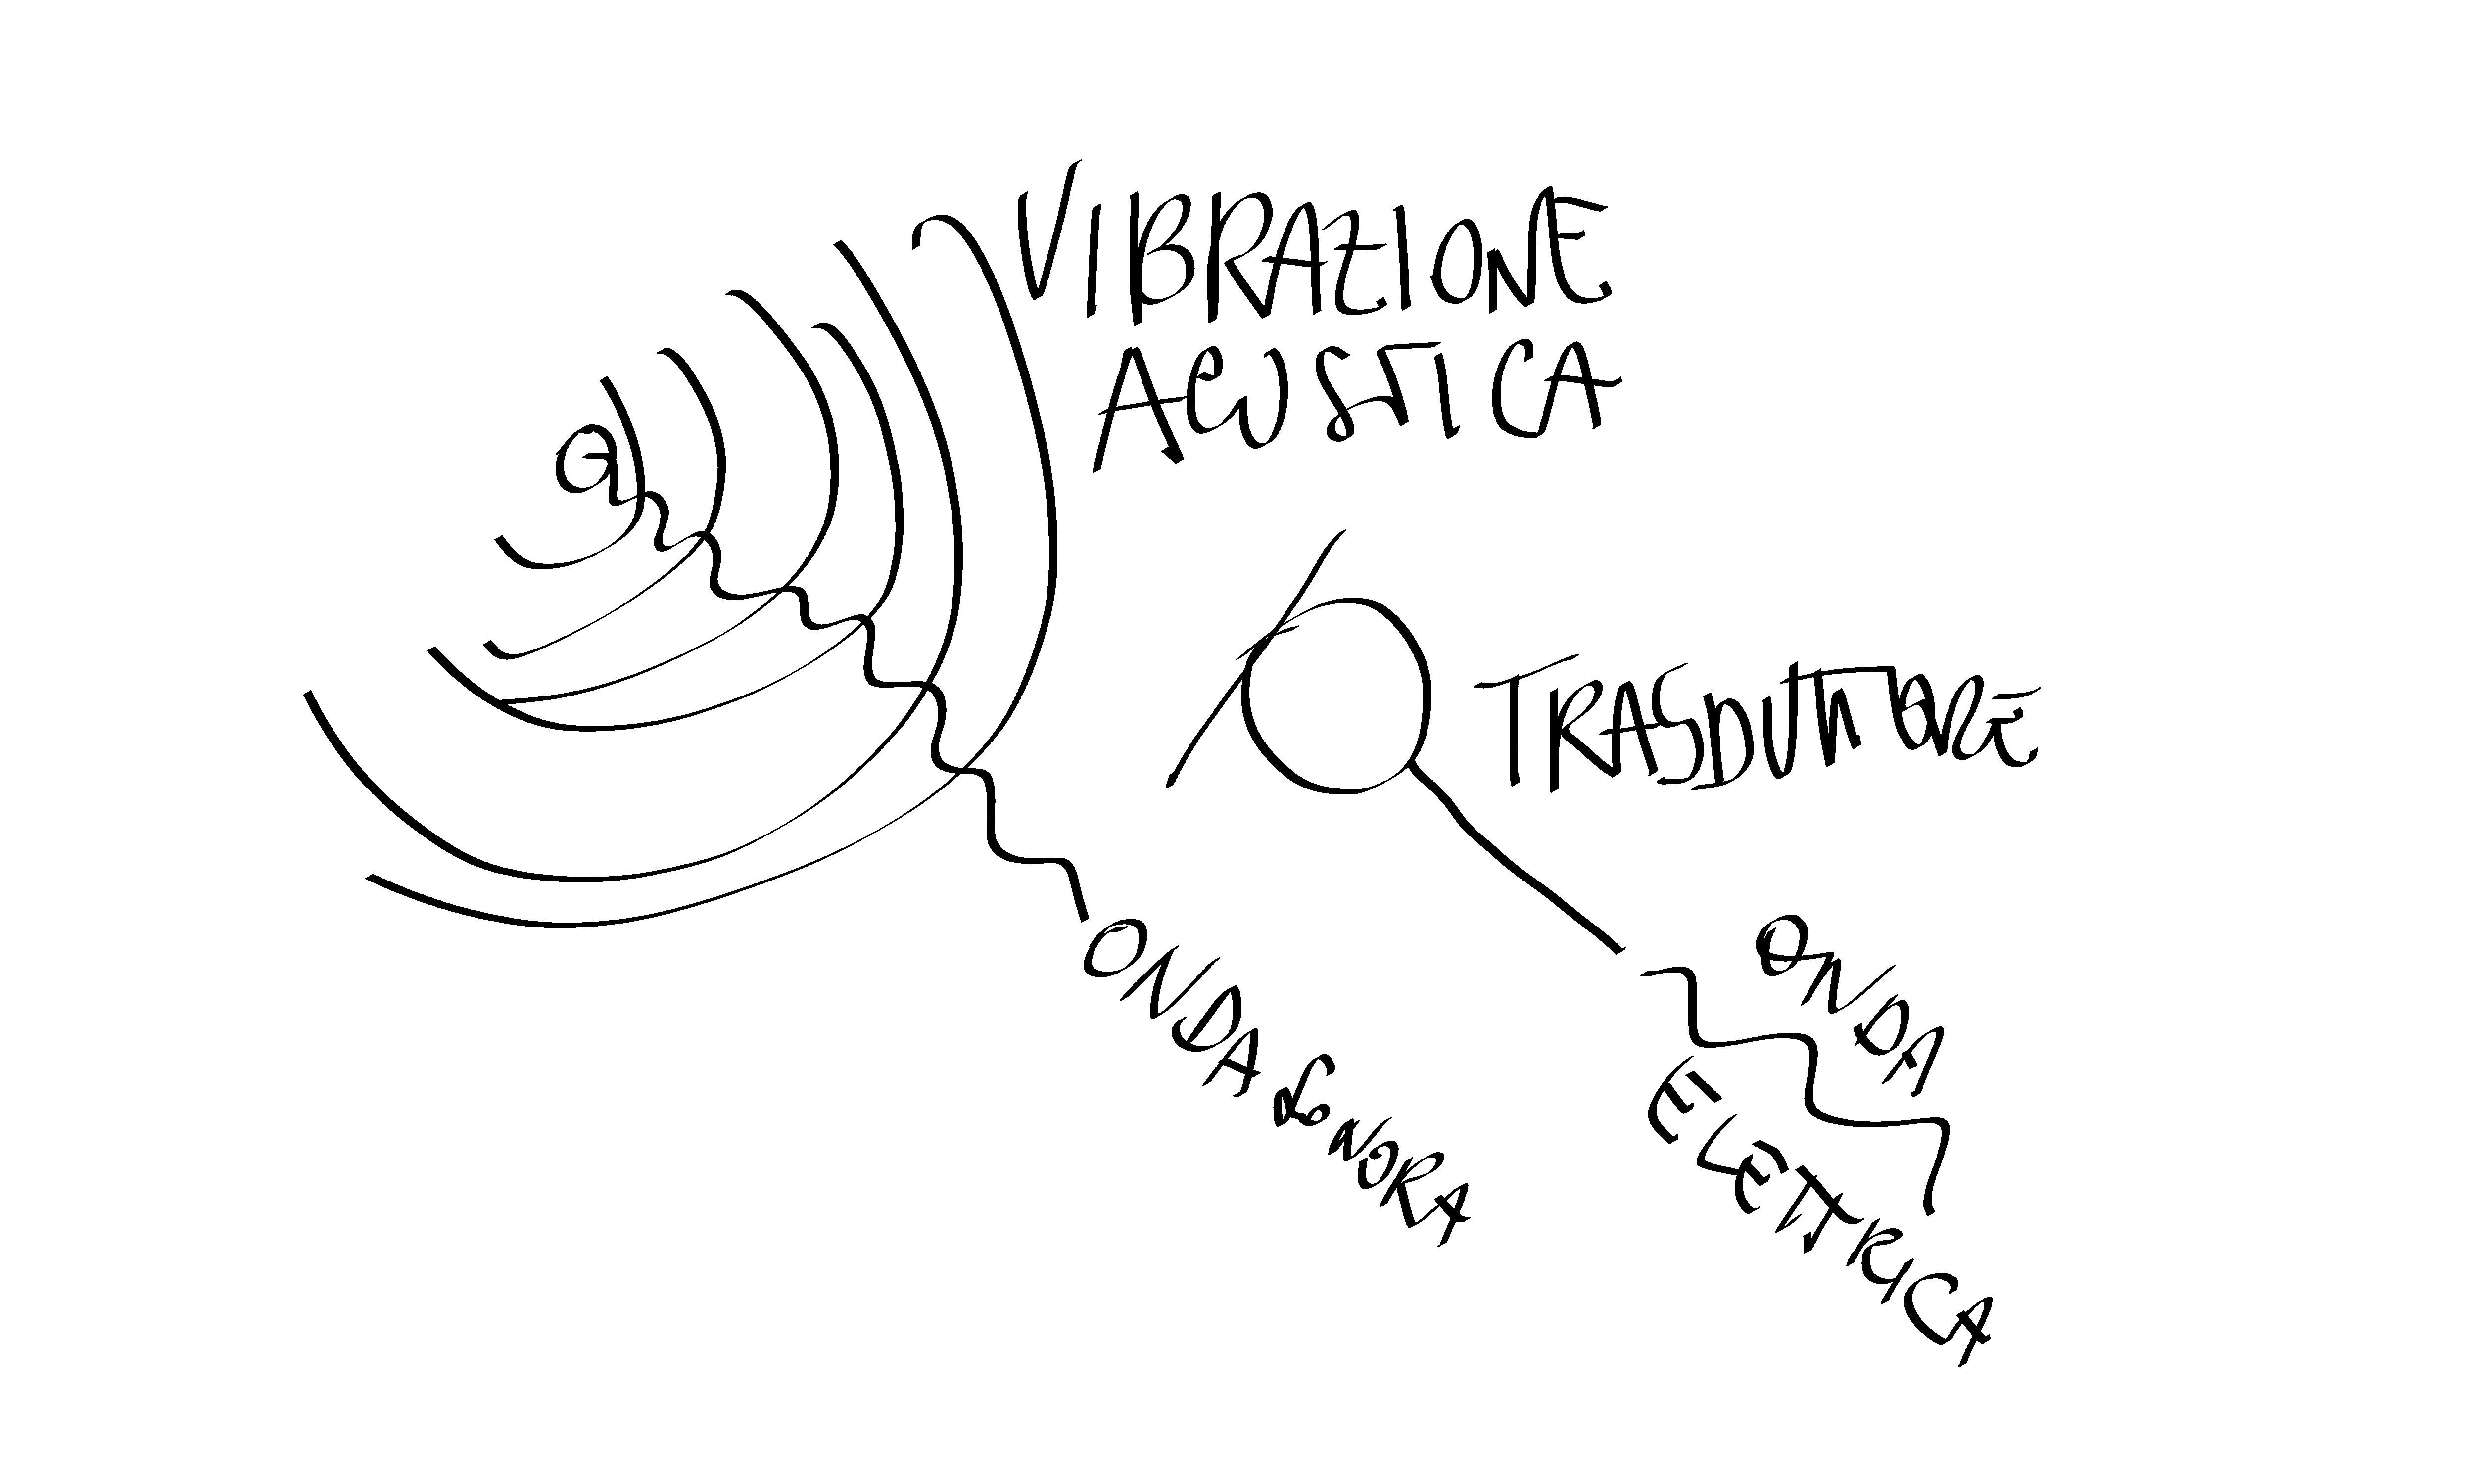
\includegraphics[width=0.99\columnwidth]{CAPITOLI/0200/img/trasduzione.png}
\caption[]{Generalizzazione di un sistema microfonico.}
\label{mic:condensatore}
\end{figure}

La generalizzazione del un microfono consiste in un sistema meccanico mobile esposto
all’onda sonora e destinato ad operare la \emph{trasduzione}\footnote{La
trasformazione della natura di un segnale operata da un trasduttóre,
derivato dall'inglese \emph{transducer} (che opera una trasduzione), dal latino
\emph{trans-ducere} (tras-portare). Il termine indica un dispositivo che converte
un segnale di data natura (acustica, elettrica, meccanica, termica, ecc.) in un
segnale di natura diversa. Si usa qualificare i t. con un aggettivo composto,
di cui la prima parte precisa la natura del segnale applicata e la seconda
parte quella del segnale d'uscita: t. acustoelettrico, che converte un suono in
un segnale elettrico (per es., un microfono), t. elettroacustico, da segnale
elettrico a suono (per es., un altoparlante). \\ – Fonte: Enciclopedia Treccani}
di una grandezza acustica, come la variazione di pressione, attraverso l'analogo
movimento meccanico rappresentato dallo spostamento della parte mobile del microfono, e da un sistema
elettrico a esso collegato destinato a operare la \emph{trasduzione} della
grandezza meccanica in una grandezza elettrica generando una una variazione di
corrente.

Tutti i microfoni si attivano attraverso una specifica amplificazione elettrica,
motivo per cui potremmo dire che li alimentiamo per copiare il campo sonoro
piuttosto che prenderne energia, sottolineando la peculiarità dell'osservazione
fisica: copiare il campo sonoro, intralciandolo.

Prima di procedere con una moderna classificazione dei microfoni, se ne può tracciare
brevemente il percorso storico.

Non si è stati bambini fortunati senza il \emph{gioco del telefono}. Muovere
un messaggio sottovoce tra file di orecchie e bocche allo scopo di tras-portare
l'informazione, sperando che questa venga tras-figurata, tra le risate. Più
felici di così solo con l'esperimento di collegare tra loro due bicchieri di carta con
uno spago per parlarsi, sottovoce, a breve distanza. È il suono mobile, nel tempo
e nello spazio, il meccanismo del suono in viaggio, che ha reso tutto possibile.

\begin{figure}[th!]
\centering
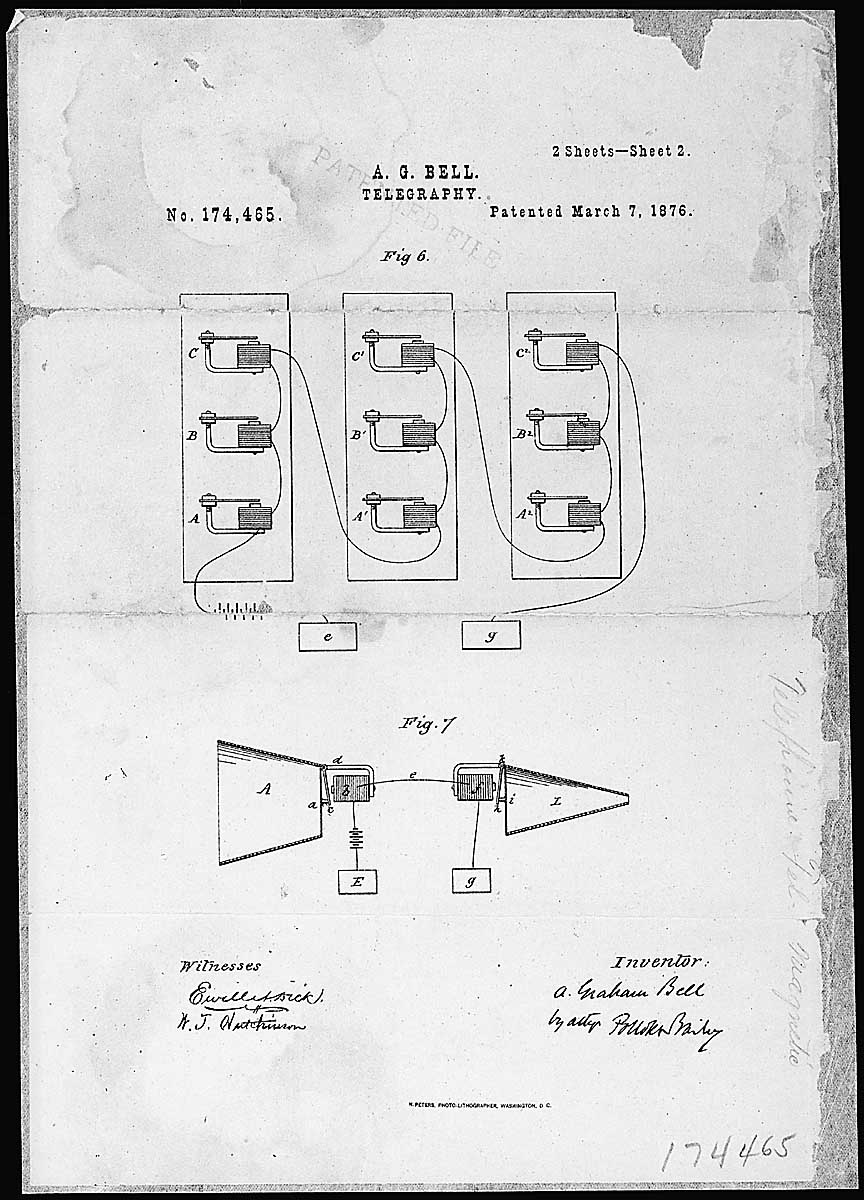
\includegraphics[width=0.99\columnwidth]{CAPITOLI/0200/img/telephone-patent-drawing-l.jpg}
\caption[]{Alexander Graham Bell.\\ Telefono. Registro brevetti: 302052.}
\label{agb:tel}
\end{figure}

Nel 1876, a Philadelphia, si teneva la \emph{Centennial Exhibition} per celebrare
il centenario della nascita della nazione. Fu la prima fiera mondiale a tenersi
negli Stati Uniti con lo scopo, tra gli altri, di annunciare a tutti che la nazione era
ufficialmente una potenza industriale. All'interno degli edifici della fiera erano
esposte le opere di due inventori: Alexander Graham Bell e Thomas Alva Edison.

\begin{figure}[th!]
\centering
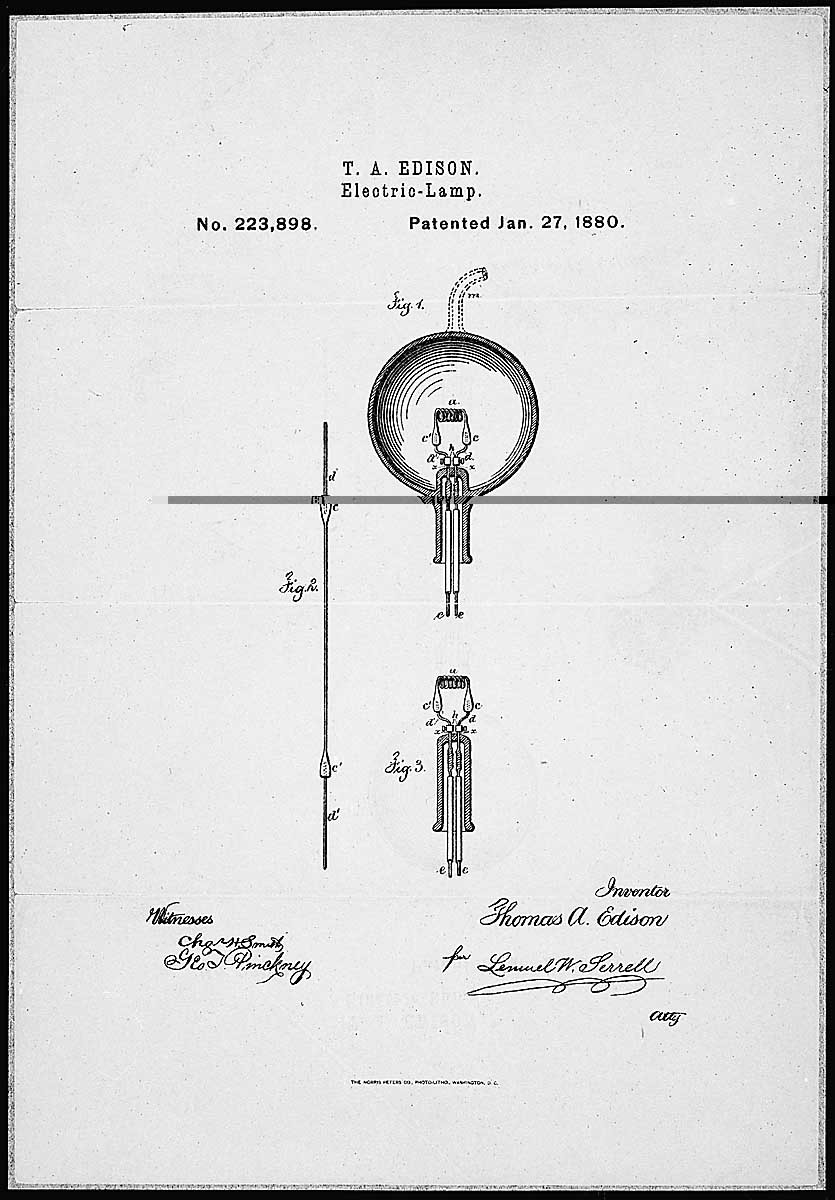
\includegraphics[width=0.99\columnwidth]{CAPITOLI/0200/img/light-patent-drawing-l.png}
\caption[]{Thomas Edison. \\ Lampada elettrica. Registro brevetti: 302053.}
\label{te:lamp}
\end{figure}

Un passo intermedio nello sviluppo della modulazione senza contatto (in aria) della
corrente continua è stato sviluppato nel 1878 da David Edward Hughes. In questa
realizzazione delle barrette di carbonio fissate ai due estremi venivano messe in
vibrazione dalle onde sonore dando luogo a una fluttuazione abbastanza grande
della resistenza
di contatto tra l'asta di carbonio e i due punti di fissaggio. Questo tipo di
microfono fu impiegato da Clement Ader nel 1881 nella sua pioneristica trasmissione a due
canali dal teatro dell'Opera di Parigi al padiglione espositivo.
Fu Hughes, per inciso, a usare per primo il termine \emph{microfono}, applicato
ai dispositivi di questo tipo.

Furono le compagnie radio-televisive a spingere nello sviluppo di queste tecnologie,
fin dagli anni venti, per aumentare la qualità del suono elettroacustico ad
entrambi gli estremi della catena: microfoni ed altoparlanti.

La compagnia \emph{Western Electric}, il ramo produttivo della \emph{Bell Telephone},
rispondendo alle esigenze crescenti sviluppava sia microfoni elettrodinamici che
a condensatore.

\begin{figure}[t]
\centering
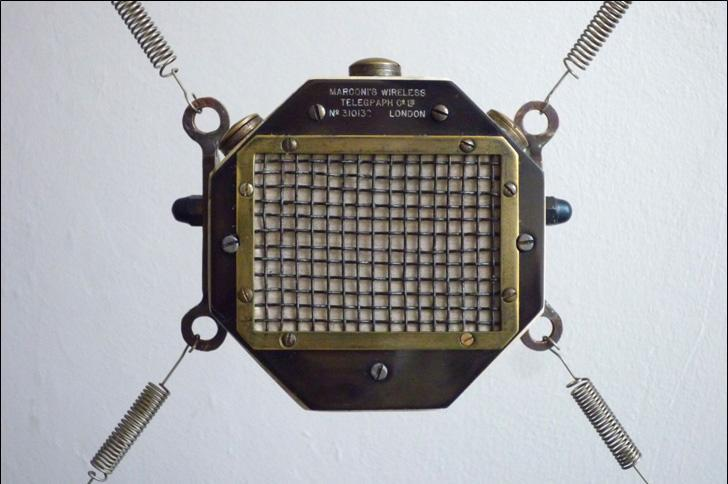
\includegraphics[width=0.99\columnwidth]{CAPITOLI/0200/img/1321872621718Reisz8.jpg}
\caption[]{Microfono \emph{Marconi-Reisz}, restauro RAI.}
\label{mic:Marconi-Reisz}
\end{figure}

Contemporaneamente in Europa Eugen Reisz stava cercando con George Neumann,
suo collaboratore, un nuovo sensore per avere un suono migliore rispetto al
microfono a dischi di carbone utilizzato nella telefonia. Le ricerche portarono alla
costruzione di un contenitore rettangolare fresato in un blocco di marmo o in
bachelite riempito di uno strato di finissimi granuli di carbone chiusi da un
diaframma non conduttore. L’involucro in marmo risulta privo di risonanze e la
cavità con i granuli di carbone è sigillata costituendo un \emph{microfono dinamico a pressione}.

Il microfono, progettato in Germania, è stato prodotto nel Regno Unito nel 1925/26
dalla \emph{Marconi Wireless}, motivo per cui è conosciuto come microfono
\emph{Marconi-Reisz} poi prodotto anche da \emph{AEG (Allgemeine Gesellschaft
Elektrik)} con piccole differenze costruttive.

Il microfono aveva una risposta in frequenza da $50Hz$ ai $1000Hz$ in modo
piuttosto lineare, estendendosi meno linearmente fino ai $10KHz$. Un microfono
di notevole qualità per quell’epoca, molto sensibile, che quindi veniva montato su un supporto elastico.

La risposta in frequenza poteva essere migliorata ulteriormente attravero un
circuito elettrico e qualche accorgimento operativo. Un'informativa interna
della \emph{BBC} del 1935 comunicava \emph{lo speaker deve
parlare attraverso il microfono ad un angolo di 45 gradi}, a sottolineare la relazione
tra dimensione del diaframma, angolo di incidenza e risposta in frequenza.
Le costruzioni successive portarono migliorie timbriche, nonostate alcune limitazioni
tra cui il livello di rumore di fondo abbastanza alto, causato dalle minuscole
scintille di scarica tra i granuli.
Un altro problema era che i granuli gravitavano verso il basso e
si compattavano. Questo produceva un livello di fruscio maggiore e una minore
sensibilità. Uno dei compiti dei tecnici audio dell’epoca era quello di passare
quotidianamente e prima di ogni programma negli studi e girare i microfoni
\emph{Reisz} a testa in giù e scuotendoli in modo da ridistribuire i granuli compattati.
Il manuale di Istruzioni del 1935 indicava che
il microfono doveva essere scollegato \emph{e, posto con il diaframma orizzontale
e rivolto verso l'alto\ldots} deve inoltre \emph{essere ben agitato da un lato all'altro in
modo da allentare il compattamento dei granuli}.

La sua uscita era comunque \emph{asimmetrica}, in quanto le onde di pressione
sonora comprimevano i granuli, ma la rarefazione non li decomprimeva.

\subsection{Architettura e principio di funzionamento}

Una prima catalogazione dei microfoni può essere effettuata per architettura,
ovvero in funzione delle caratteristiche costruttive che ne determinano i
risultati in termini di trasduzione.

In questa classificazione troviamo:

\begin{compactitem}
  \item microfoni dinamici
  \item microfoni a nastro
  \item microfoni a condensatore
  \item microfoni a condensatore electret
\end{compactitem}

\subsubsection{Microfoni dinamici}

Il microfono dinamico, indicato anche a bobina elettrodinamica,
elettromagnetica o mobile, si basa sul principio dell'induzione magnetica in cui
il conduttore, nel caso specifico l'avvolgimento di filo della bobina, si muove
attraverso un campo magnetico inducendo una tensione proporzionale alla forza
del campo magnetico, alla velocità del movimento e all'ampiezza del movimento
lungo il campo magnetico.

\begin{figure}[h]
\centering
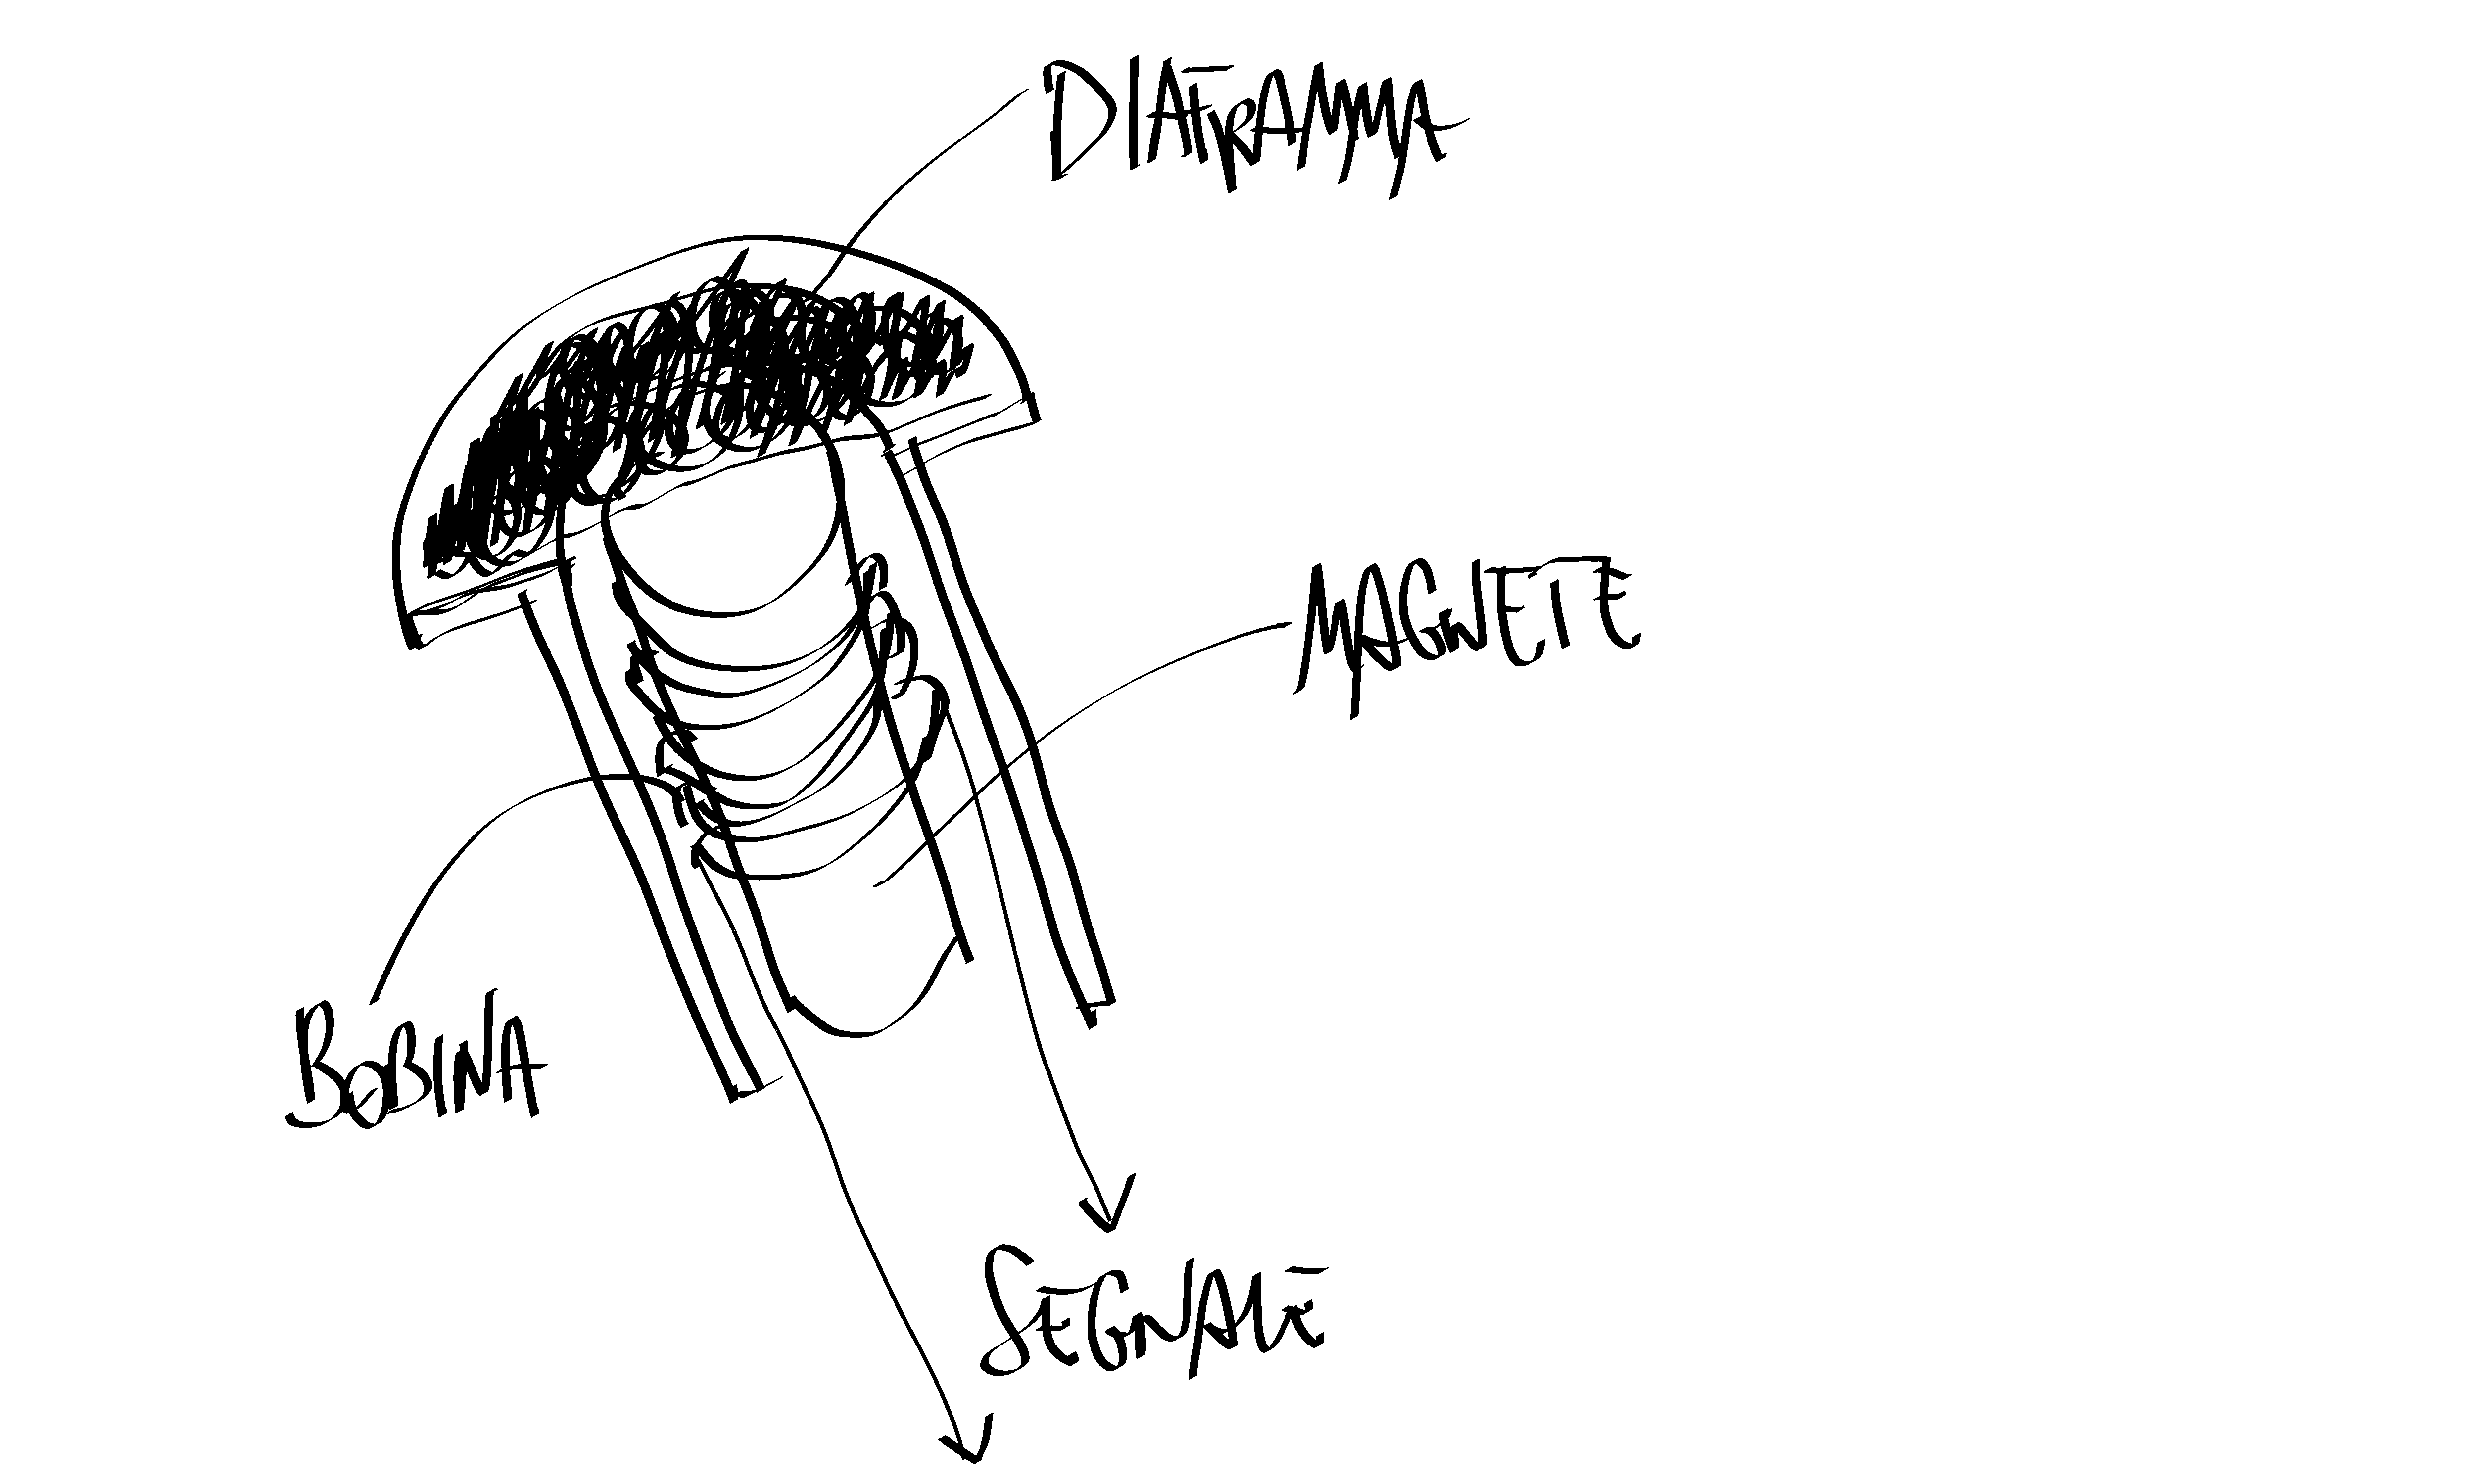
\includegraphics[width=0.99\columnwidth]{CAPITOLI/0200/img/mic-dinamic.png}
\caption[]{Microfono dinamico.}
\label{mic:dinamico}
\end{figure}

%A tale famiglia appartengono microfoni, la cui architettura è schematizzata in fig. 1,

Il diaframma circolare messo in vibrazione dalle onde sonore trasmesse nell’aria
è solidale con l'avvolgimento di filo di rame della bobina, libero di muoversi
all’interno di un campo magnetico costituito da un magnete permanente.

Le onde sonore, costituite da compressioni e rarefazioni dell’aria secondo una
determinata frequenza (corrispondente all’altezza del suono), vengono perciò
trasformate, attraverso tale trasduttore, in corrente elettrica, presente sui
cavi di uscita alle estremità dell’avvolgimento di rame, con variazioni di
ampiezza e frequenza analoghe a quelle delle onde acustiche. Questo
principio di trasduzione, come vedremo in seguito, non è altro che il
procedimento inverso a quello della maggior parte degli altoparlanti: in quel
caso, una corrente elettrica proveniente dall’amplificatore si presenta ai
poli estremi di una bobina mobile, anch’essa libera di muoversi all’interno di
un campo magnetico, e genera una corrispondente vibrazione sul cono
dell’altoparlante solidale alla bobina.

Le caratteristiche salienti di questo tipo di microfono sono:

\begin{compactitem}
  \item estrema robustezza ed affidabilità
  \item segnale di uscita molto basso
  \item risposta rimbrica limitata in banda
  \item scarso rapporto tra segnale e rumore
\end{compactitem}

È importante osservare come, a causa dell’elasticità e della massa del materiale
vibrante, il gruppo diaframma-bobina abbia una sua frequenza di risonanza
caratteristica. Al di sotto di tale frequenza il comportamento è dettato dal
rapporto elasticità/rigidità, mentre al di sopra dipende dalla massa del
complesso vibrante. Questo è uno dei motivi per cui i microfoni dinamici
tendono a \emph{colorare} il suono quando l'altezza in entrata si muove attorno
alla frequenza di risonanza, e tendono ad avere anche una risposta non perfettamente
estesa alle alte frequenze, a causa dell’inerzia delle masse in movimento.
Il rapporto tra qualità del segnale è proporzionale al numero degli avvolgimenti
della bobina, per cui il vantaggio della riduzione delle masse vibranti è
controbilanciato da un segnale di uscita inferiore, con conseguente diminuzione
del rapporto segnale/rumore. La soluzione risiede nel compromesso tra i valori
ottimali di tutti questi parametri.

L'evoluzione dei materiali nel campo dell'elettroacustica ha portato l'introduzione
nei sistemi dinamici (magnetici) del neodimio, utilizzato sia nei sistemi di
diffusione che di ripresa. La qualità del neodimio è nell'essere un materiale ad
alta coercitività, consentendo l’utilizzo di bobine a massa ridotta, a tutto
vantaggio della risposta alle alte frequenze.

\subsubsection{Microfoni a nastro}

In questo tipo di microfono il principio di funzionamento è assimilabile a
quello del microfono dinamico, con la differenza che la parte vibrante nonn è
costituita da un diaframma solidale ad una bobina mobile, bensì è costituito
da un sottilissimo foglio di alluminio
ondulato, anch’esso libero di vibrare tra i poli di un magnete permanente, e
alle estremità del quale si produce una tensione elettrica corrispondente alle
onde sonore in entrata. In questo tipo di microfono le funzioni
di vibrazione e di trasduzione sono svolte dallo stesso elemento fisico.

\begin{figure}[h]
\centering
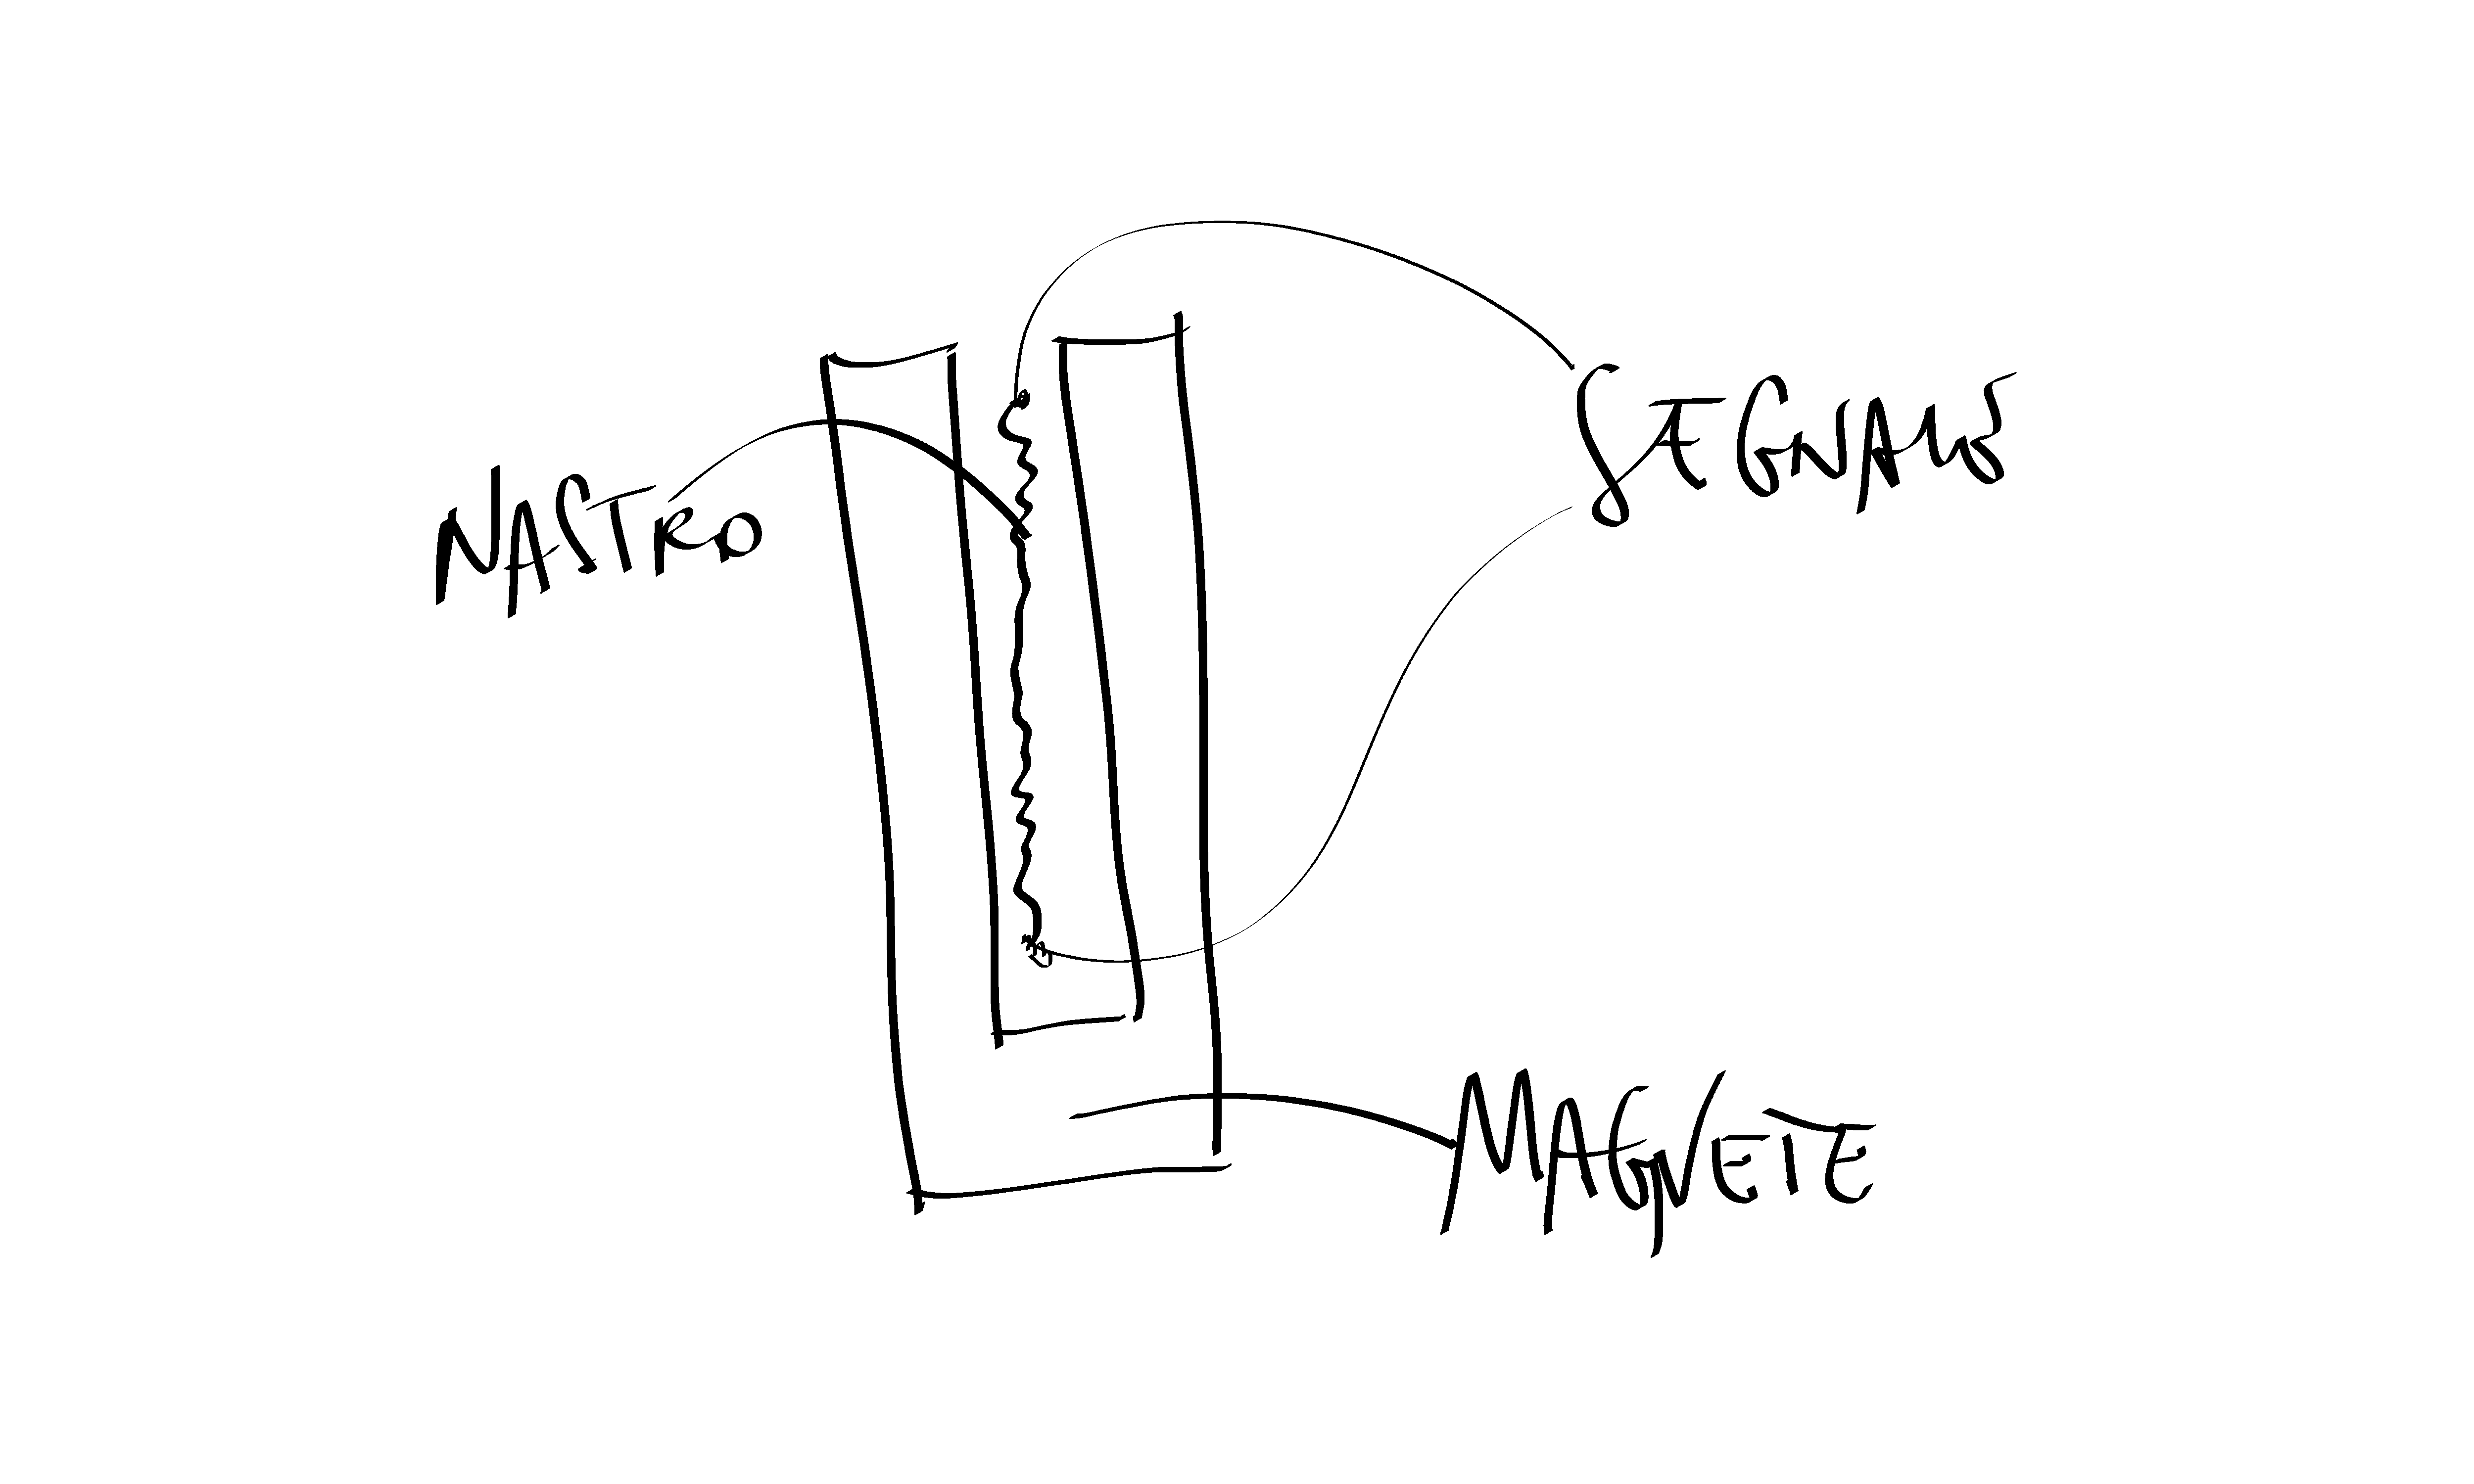
\includegraphics[width=0.99\columnwidth]{CAPITOLI/0200/img/mic-nastro.png}
\caption[]{Microfono a nastro.}
\label{mic:nastro}
\end{figure}

I primi microfoni a nastro erano piuttosto grandi, con magneti pesanti ed
inefficienti. Inoltre era piuttosto conosciuta la fragilità del nastro.

Le caratteristiche timbriche del microfono a nastro sono:

\begin{compactitem}
  \item assenza di coloratura dovuta alla frequenza di risonanza situata molto
  più in basso rispetto ai microfoni dinamici (inferiore ai $40Hz$);
  \item risposta estesa sulle alte frequenze a causa della ridotta massa del
  diaframma vibrante.
\end{compactitem}

Essendo il segnale d’uscita di livello estremamente basso,
ed essendo bassa anche l’impedenza di uscita, viene interposto un trasformatore
per elevarlo di intensità e fornire un’impedenza conforme allo standard.
La sottigliezza del nastro vibrante è inoltre causa di fragilità del dispositivo,
rendendolo inadatto alla microfonazione di segnali dotati di un’elevata pressione
sonora. Caratteristica di questo tipo di microfono è la naturale risposta bi-polare,
denominata figura-8, che sarà meglio descritta in seguito.

\subsubsection{Microfoni a condensatore}

Edward Christopher Wente iniziò a lavorare per la Western Electric nel 1914
sulla ricerca che prevedeva la progettazione e la calibrazione di un
trasmettitore (o microfono) uniformemente sensibile da utilizzare in laboratorio.
I microfoni a disco di carbone utilizzati nei ricevitori telefonici avevano una
risposta in frequenza troppo stretta, irregolare e un rumore di fondo eccessivo
per poter essere applicati nella ricerca sul suono. Con l'utilizzo
dell'amplificatore valvolare di Harold Dean Arnold, nel 1916, Wente produsse il
primo microfono a risposta in frequenza piatta da lui denominato trasmettitore a
condensatore. L'anno successivo pubblicò i suoi risultati in
un articolo teorico su \emph{The Physical Review}. Nel 1922, produsse un
trasmettitore a condensatore con una sensibilità cento volte maggiore, il che
era abbastanza per renderlo un dispositivo pratico, sebbene la sua alta
impedenza richiedesse il collegamento diretto ad un preamplificatore valvolare.

Il microfono a condensatore moderno è molto simile ai modelli originari di Wente
del 1917, solo molto più piccoli e raffinati nella costruzione. Spesso si fa
conusione nel riferirsi, in lingua inglese, a tale microfono attraverso il termine
\emph{condenser microphone}, tuttavia il termine rivela delle ambiguità e già
dagli anni venti del novecento ci si è riferiti alla tecnologia nei termini
di \emph{capacitor microphone}.

\begin{figure}[h]
\centering
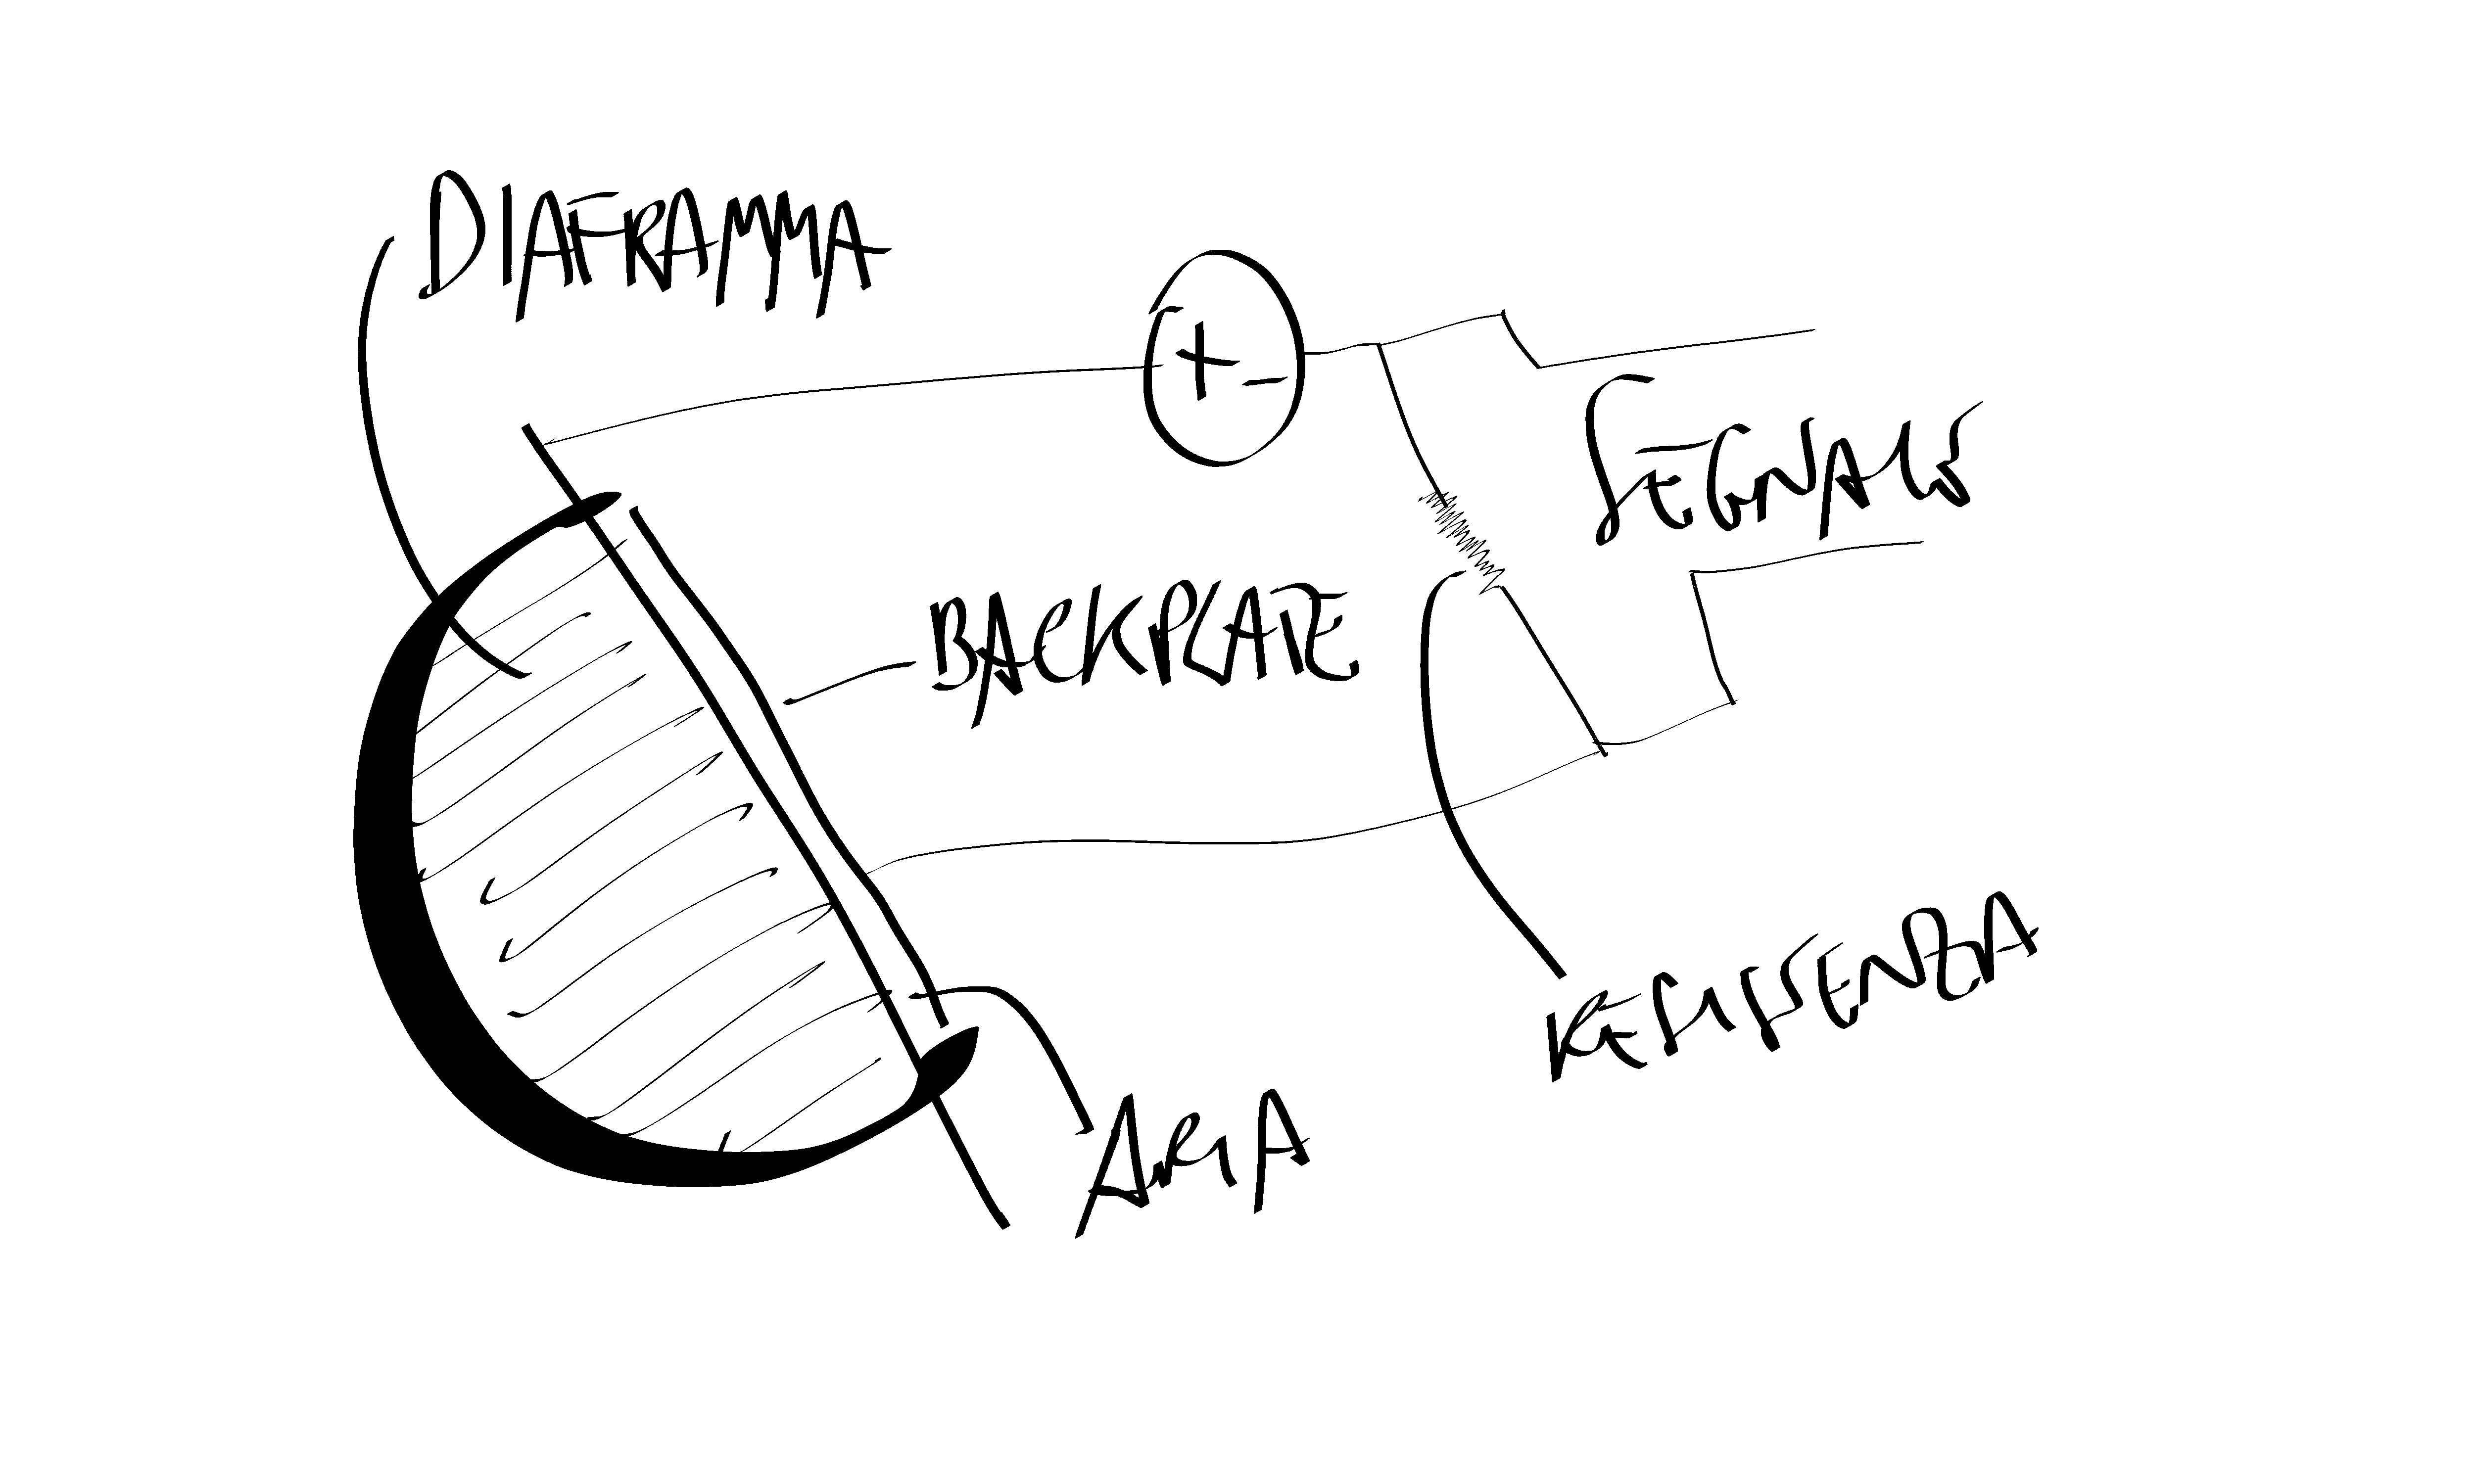
\includegraphics[width=0.99\columnwidth]{CAPITOLI/0200/img/mic-capacitor.png}
\caption[]{Microfono a condensatore.}
\label{mic:condensatore}
\end{figure}

Il microfono a condensatore è costituito da un diaframma (solitamente in materiale
plastico o metallico molto leggero come alluminio, nickel e titanio)
rivestito finemente d'oro. La lamina è distanziata da una seconda lamina fissa, più spessa,
denominata \emph{backplate} (lamina posteriore) che può essere forata. Le due
lamine hanno tra loro una differenza di potenziale in quanto
viene applicata una tensione di polarizzazione in corrente continua ad una delle
due.

\begin{figure}[tbhp]
\centering
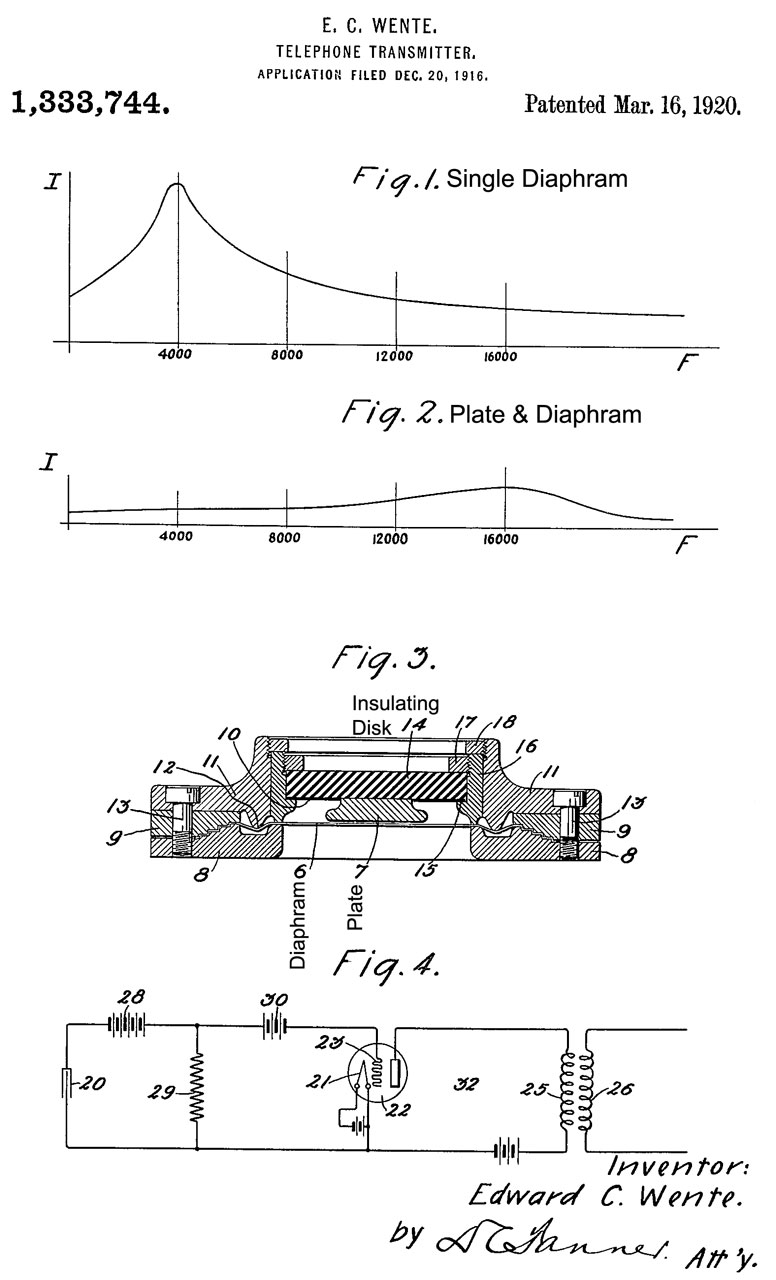
\includegraphics[width=0.99\columnwidth]{CAPITOLI/0200/img/US1333744-1b.jpg}
\caption[]{Edward Christopher Wente. \\ Microfono a condensatore. Registro brevetti: 1333744.}
\label{mic:wentemic}
\end{figure}

Il condensatore è un elemento elettronico passivo pre-polarizzato, in grado di
bloccare il passaggio di corrente alternata attraverso i conduttori tra i quali
è posizionato un diverso tipo di dielettrico. Quando esiste una differenza di
potenziale (tensione) tra i conduttori, viene generato un campo elettrico
statico che viene separato dal dielettrico tra cariche positive e negative
memorizzate rispettivamente sul polo positivo e negativo del condensatore.

Secondo il principio di funzionamento del condensatore, la vibrazione fa
quindi variare periodicamente la distanza tra le due lamine, generando una
corrispondente variazione periodica del campo elettrico e la conseguente
generazione di un’onda in uscita. Questa tecnica circuitale è nota come
“polarizzazione in corrente continua” (DC-biased), ed è differente da un’altra
tecnica, ossia la circuitazione RF (radiofrequenza). Quest’ultima prevede
un’oscillatore ad alta frequenza (in funzione di portante), rispetto al quale
il condensatore costituito dal corpo diaframma-backplate agisce in funzione
modulante. Il segnale verrà successivamente demodulato in bassa frequenza
restituendo il segnale elettrico originale. Il vantaggio di questo tipo di
circuitazione consiste in una riduzione del rumore di fondo generato dal
circuito di preamplificazione (inherent noise).

La circuitazione attiva all'interno di questo tipo di microfono necessita di
un'alimentazione esterna fornnita attraverso il sitema noto come alimentazione
fantasma (\emph{phantom power}), che consiste nel far viaggiare sul
cavo microfonico una determinata quantità di corrente continua. In alcuni casi
questa può essere fornita anche da dispositivi a batteria o da batterie interne
al corpo microfonico. Tale alimentazione consente inoltre di installare,
sempre all’interno del corpo microfono, un circuito di preamplificazione,
indispensabile, dato il bassissimo voltaggio generato dalle lamine, a fornire
un segnale d’uscita di livello adeguato.
In virtù di queste caratteristiche il microfono a condensatore offre:

\begin{compactitem}
  \item un segnale d'uscita efficace
  \item una curva di risposta in frequenza molto ampia
  \item elevata sensibilità
\end{compactitem}

Rispetto al microfono dinamico, offre un segnale d’uscita maggiore ed una migliore curva di
risposta in frequenza, contro una robustezza inferiore ed un costo decisamente superiore.

\subsubsection{Microfoni a electret}

La richiesta di tensione esterna necessaria alla polarizzazione del microfono a
condensatore ha rappresentato per molti hanni un ostacolo. In alcuni
contesti i grandi e pesanti preamplificatori potevano rappresentare uno svanntaggio
nella scelta del microfono. Agli inizi degli anni sessanta, presso i laboratori
Bell Telephone, Sessler e West descrissero un microfono a condensatore che utilizzava
materiale dielettrico permanentemente polarizzato, tra il diaframma mobile ed la
piastra posteriore (back-plate). I primissimi materiali utilizzati persero
sensibilità nel tempo, ma lo sviluppo di quella tecnologia ha portato risultati
ora molto stabili e paragonabili a quelli dei tradizionali microfoni a condensatore.

\begin{figure}[h]
\centering
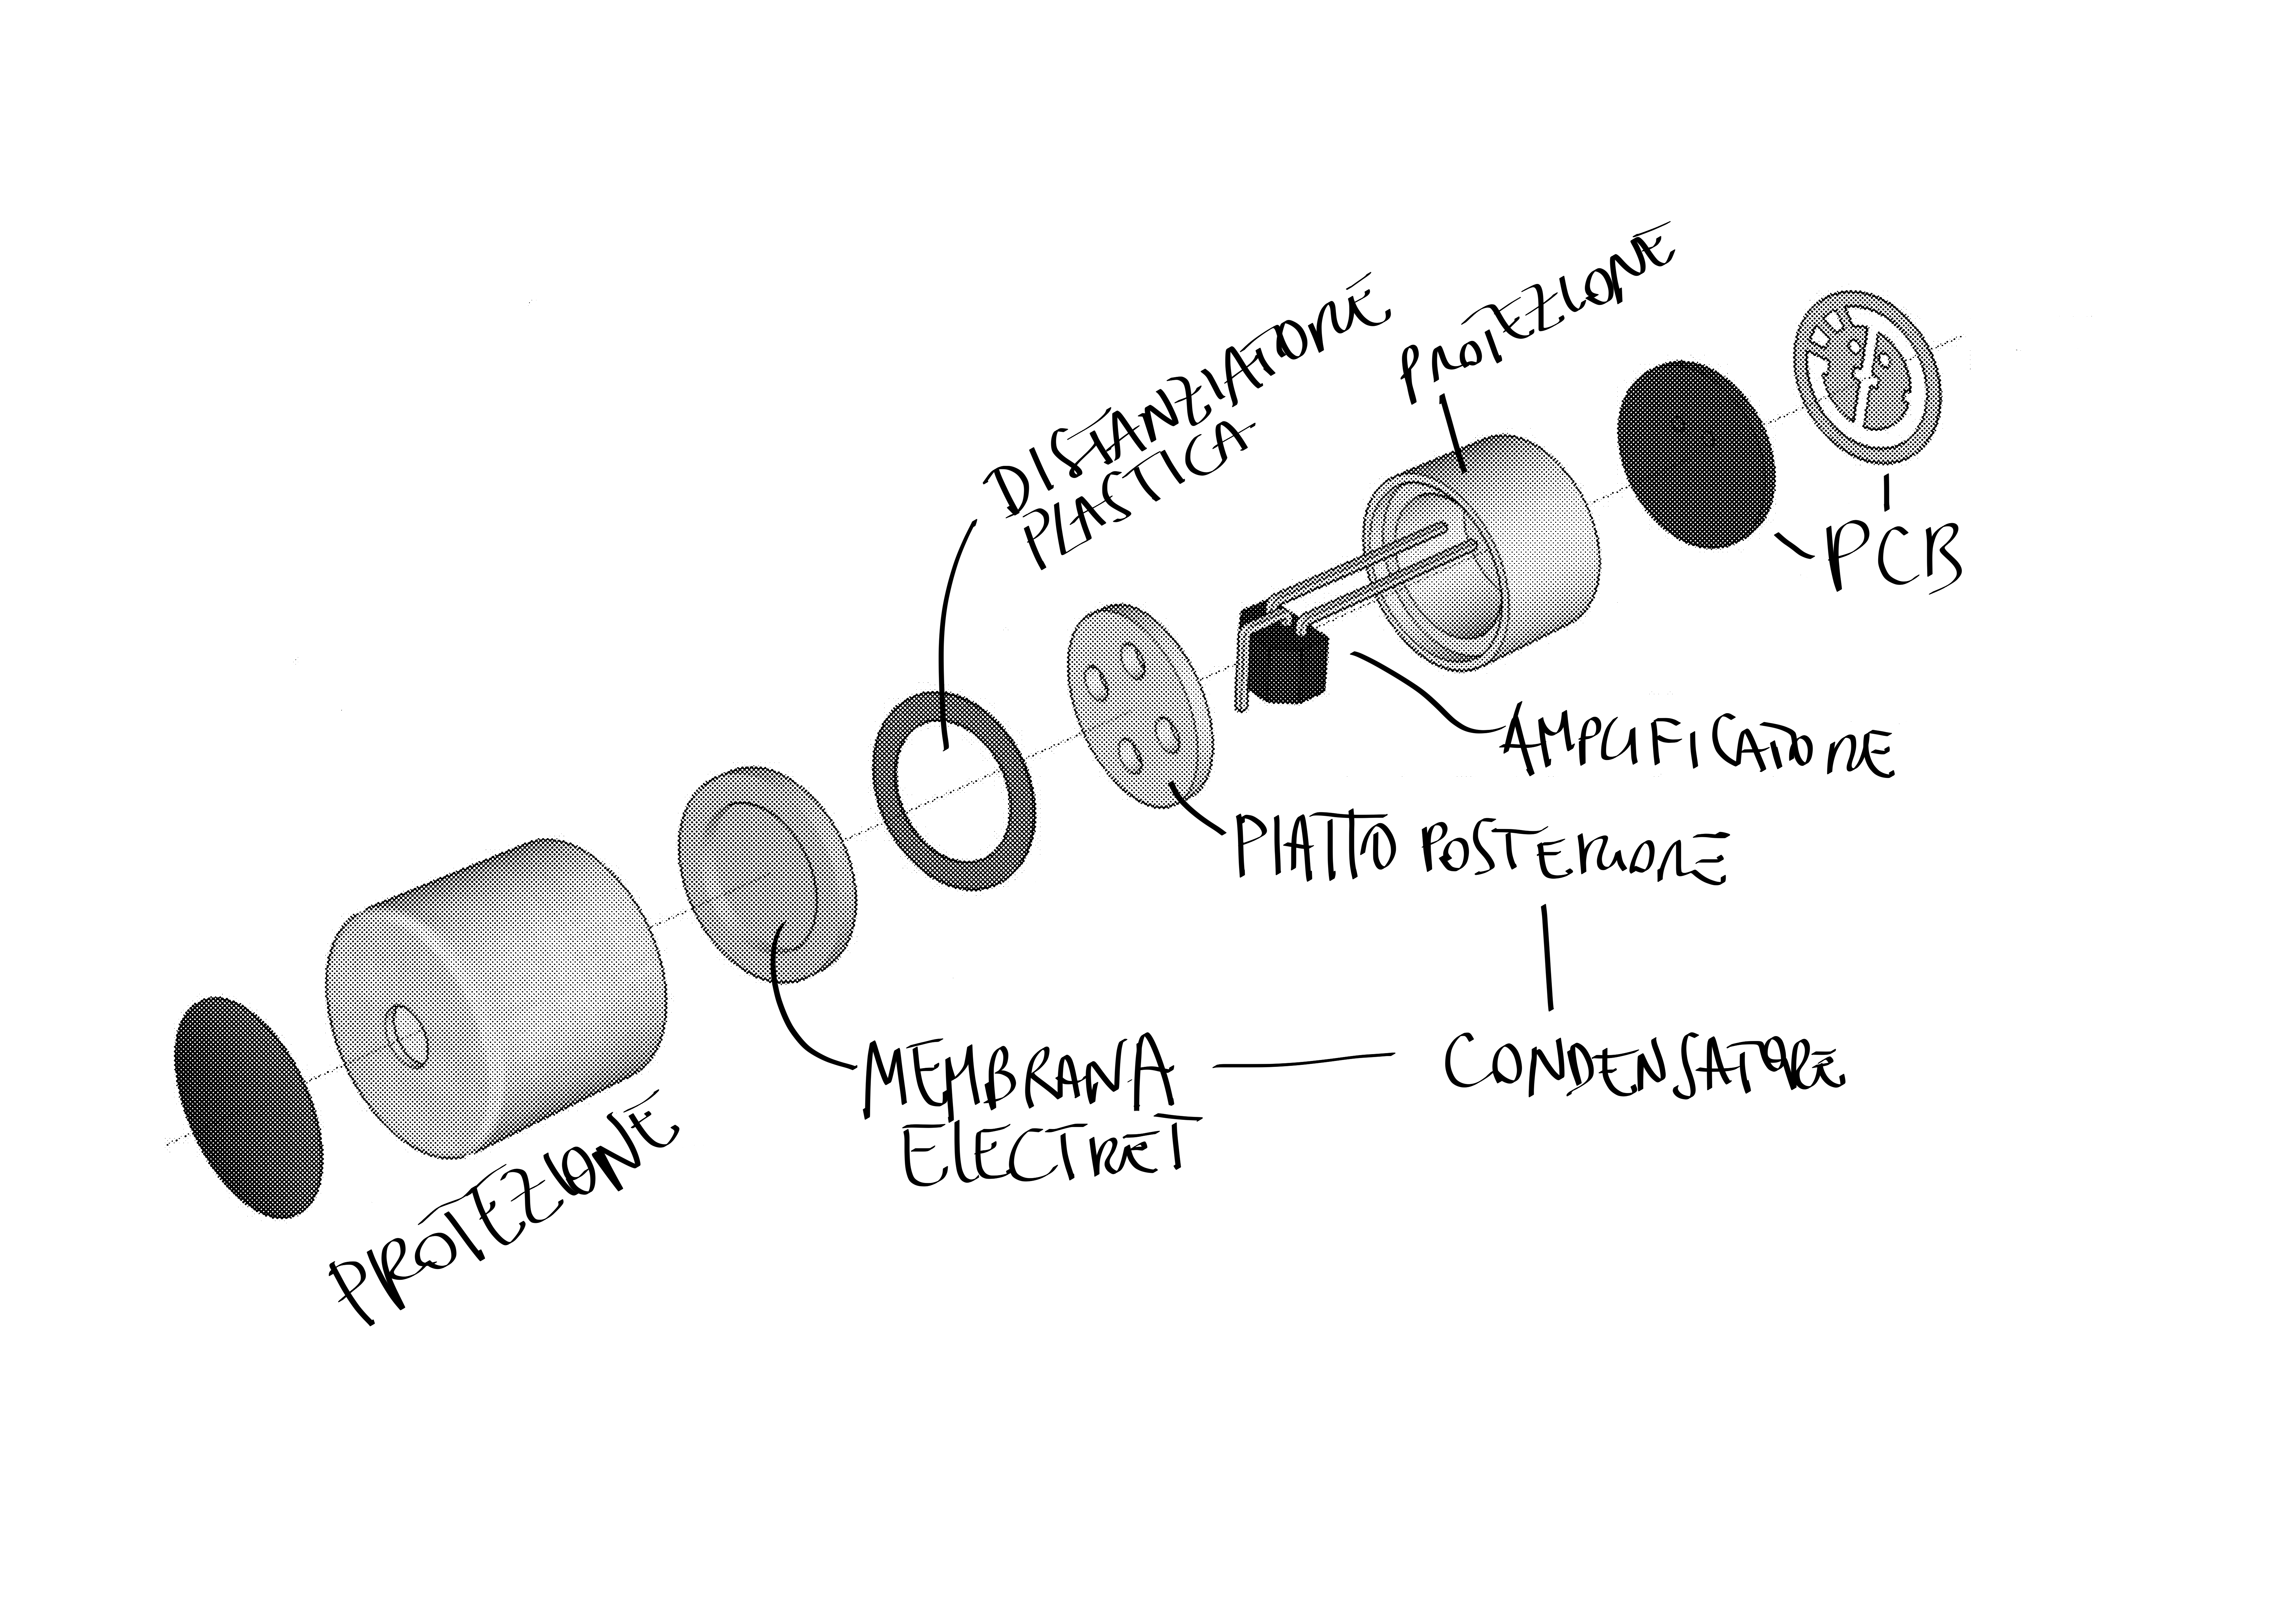
\includegraphics[width=0.99\columnwidth]{CAPITOLI/0200/img/electret.png}
\caption[]{Microfono a condensatore electret.}
\label{mic:electret}
\end{figure}

Il microfono a condensatore di tipologia \emph{electret} è quindi a tutti gli effetti
considerabile una variante nel campo dei microfoni a condensatore (\emph{ECM,
Electret Condenser Microphone}). La particolarità di questi microfoni è che tra
il diaframma e il backplate è inserito un dielettrico di materiale isolante
(electret) il quale ha la caratteristica di essere pre-polarizzato
elettricamente, in modo simile ad un magnete permanente nel campo del magnetismo.
In tal modo, il diaframma non necessita della tensione di polarizzazione,
sebbene questi microfoni siano comunque dotati di un circuito di preamplificazione,
per cui possono essere alimentati da alimentazione fantasma molto bassa o da batteria.
Sebbene questa tecnica sia sorta con l’intento di abbassare i costi, e
quindi sia stata implementata in prodotti economici rivolti più alle registrazioni
amatoriali che a quelle professionali, i progressi effettuati la collocano ormai
quasi alla pari con i migliori microfoni a condensatore. Tra i microfoni electret
i migliori sono da considerarsi quelli dove il dielettrico è solidale con il
backplate, che ne costituisce una delle superfici: essi prendono il nome di
\emph{back-electret}.

% Nella fig. 4 vediamo lo schema in sezione di un microfono electret, e possiamo
% notare come l’esiguità dei componenti lo rendano un dispositivo estremamente
% adatto alla miniaturizzazione, quindi adatto, ad es., ai microfoni a clip.

% \subsubsection{Parametri elettrici}
%
% A chiusura di questa panoramica sull’architettura dei microfoni occorre fornire
% qualche elemento sui parametri elettrici forniti a corredo dei microfoni. Oltre
% alle caratteristiche polari, di cui si parlerà di seguito, i valori più
% significativi per la valutazione di un microfono “sulla carta” sono:
%
% 1) La sensibilità
% 2) Il rumore
% 3) L ’impedenza
% 4) La risposta in frequenza
%
% La sensibilità indica il livello di segnale elettrico che il microfono pu
% fornire a fronte di una determinata pressione acustica sonora. Questo parametro
% ci fornisce un’indicazione utile per determinare quanto il segnale che il
% microfono produce dovrà essere amplificato negli stadi successivi. Così ad es.
% un microfono dinamico può fornire la seguente indicazione di sensibilità:
%
% 2 mV/Pa
%
% ossia 2 millivolt per una pressione acustica sonora di 1 Pascal2. Diamo di seguito,
% indicativamente, una tabella comparativa delle tipologie di microfoni presi in esame:
%
% Il parametro per valutare il rumore introdotto da un microfono è noto come
% “Equivalent Noise Level” (anche “self-noise level”, ossia il rumore inerente
% al microfono), e si riferisce ad un livello di pressione sonora che corrisponde
% al rumore interno del microfono, ossia al suono di livello minimo che è
% possibile registrare con un dato microfono. La scala di misurazione è quella
% del dBSPL , che sarà trattato in altra lezione, ed i metodi di misura sono
% generalmente di due tipi, in base alla curva di pesatura che viene applicata:
% 1) la scala dB(A), complementare delle curve isofoniche di Fletcher-Munson,
% mediante la quale i valori ottimali per i microfoni sono quelli al di sotto di
% 15 dB;
% 2) la scala CCIR 468-1, anche nota come ITU-R 468, che differisce dalla curva
% (A) per una maggiore enfasi nella zona da 5KHz a 8KHz, che fornisce valori
% ottimali al di sotto di 25-30 dB.
%
% In fig. 5 possiamo confrontare le due curve.
%
% L’impedenza del microfono (vedi fig. 6), di cui abbiamo già trattato,
% rappresenta quel valore resistivo che viene “visto” dall’apparecchio collegato
% in successione (preamplificatore, mixer, ecc.).
%
% Come si può osservare in tab. 2, il valore tipico dei microfoni professionali
% è di 200 Ohms, ma con oscillazioni che possono andare da 50 a 600 Ohms.
%
% Risposta in frequenza
%
% Vi sono diversi modi di rappresentare il comportamento di un microfono rispetto
% alle frequenze dei suoni in entrata e rispetto all’angolo d’incidenza degli stessi.
% Uno di questi, la curva di risposta in frequenza, rappresentato in fig. 7, è un
% grafico dove i parametri sono dati dall’ampiezza del suono (sull’asse verticale)
% e dalla sua frequenza (sull’asse orizzontale), e dove i diversi angoli, ch
% rappresentano la quantificazione dello scostamento della provenienza del suono
% rispetto all’asse, sono rappresentati da una famiglia di curve, in cui ad ogni
% curva è associato un valore angolare.
%
%   Curve polari
%
% Il diagramma polare (o curva polare) è invece un grafico a disegno circolare dove i parametri sono dati dall’ampiezza e dall’angolo d’incidenza, mentre le frequenze sono rappresentate da famiglie di curve. In presenza di un’unica curva, si intende che questa è riferita ad una frequenza di 1 KHz.
% Il disegno nella parte sinistra di fig. 8 rappresenta la struttura di un tipico microfono a pressione (pressure microphone) omnidirezionale, mentre nella parte destra è rappresentata la sua curva polare, dove vediamo che la direzionalità del suono inizia ad essere percepita dal microfono a partire da circa 5 KHz in su, mentre le frequenze gravi non sono indicate in quanto assimilabili a quella rilevata a 1 KHz, cioè con attenuazione zero per qualsiasi angolo di provenienza del suono.
%
% Per comprendere il principio di funzionamento di un microfono a pressione dobbiamo immaginare il diaframma di un microfono, sia esso dinamico o a condensatore, come la pelle di un tamburo tesa sopra un contenitore ermeticamente chiuso (backchamber, in figura) Avremo quindi un dispositivo che oscilla in presenza di variazioni di pressione provenienti esclusivamente dall’esterno, essendo la parte interna a pressione costante. Tale trasduttore è per questo motivo chiamato microfono a pressione, ed essendo le variazioni di pressione indipendenti dall’angolo di arrivo delle stesse, la caratteristica polare fa di questo dispositivo un microfono omnidirezionale.
% La possibilità di reagire in modo uniforme ad ogni direzione di provenienza del suono è in realtà teorica, come si può perfettamente osservare guardando la sua curva polare, in quanto per il principio della diffrazione acustica le frequenze della gamma alta tenderanno ad attenuarsi al crescere dell’angolo di incidenza a partire dall’asse del microfono, mentre tenderanno ad elevarsi al diminuire dello stesso angolo di incidenza, ossia man mano che l’angolo di arrivo va a coincidere con l’asse. Il fenomeno è dovuto
%
% alla presenza fisica del microfono stesso nel campo sonoro che interferisce con la propagazione delle onde sonore. Un microfono che, per la sua costruzione fisica, dovuta essenzialmente al ridotto diametro del diaframma, sia esente da questo fenomeno è detto microfono a campo libero (free-field microphone). Un microfono a pressione può lavorare come microfono a campo libero nel momento in cui gli venga applicata una correzione acustica e/o una equalizzazione (free-field correction) che rendano il suo comportamento lineare alle frequenze alte.
% La caratteristica di esaltazione delle frequenze alte in asse è stata, nel corso della storia, sfruttata al fine di ottenere la linearità che si perde naturalmente con la distanza per via della densità dell’aria, che tende a penalizzare proprio le frequenze alte. Nella fig. 9 vediamo un esempio di applicazione di sfruttamento del fenomeno col microfono Neumann M50, in cui il diaframma è incastonato in una forma sferica, con l’intento di interferire maggiormente col campo libero. Nella parte destra vediamo la sua curva caratteristica, che lo hanno reso una scelta preferita nelle riprese panoramiche di orchestre.
%
% Nella fig. 10 abbiamo la rappresentazione di una curva sensibilmente differente dalla prima, in quanto vediamo che l’attenuazione del segnale ha il suo punto massimo a 180° (alle spalle del microfono), ed è già significativa (circa 12 dB) a 500 Hz. Tale curva polare descrive il comportamento di un microfono direttivo noto come microfono cardioide. Il termine
%
%
% “cardioide” deriva dalla forma a “cuore rovesciato” che tende ad assumere la curva polare.
%
% E’ importante evidenziare che la direzionalità del microfono è ottenuta mediante l’apertura, alle spalle del diaframma, di fessure la cui funzione è di far pervenire parte del suono sul retro del diaframma, generando un’opposizione di fase in grado di agire sui suoni laterali e posteriori, come illustrato in fig. 11.
% In conseguenza del fatto che il diaframma è aperto nella zona retrostante, il microfono è detto microfono a gradiente di pressione (pressure gradient microphone), in quanto la sua risposta è generata dal rapporto della pressione frontale con quella posteriore.
% Dal momento che il percorso che compie il suono in entrata alle fessure laterali è un percorso finito, mentre i suoni possono avere frequenze diverse, l’opposizione di fase è “accordata” sulle frequenze medio-alte per evidenziare la direttività. A causa di ciò esiste un effetto collaterale derivante da questa tecnica, consistente nel fatto che, nel momento in cui il microfono direzionale è installato molto vicino alla fonte sonora, si genera un’esaltazione innaturale delle frequenze gravi, dovuta proprio alla presenza delle aperture laterali. Questo effetto, che può anche essere adoperato in modo appropriato per ottenere un suono particolarmente “caldo” ad es. nella voce, prende il nome di effetto di prossimità (proximity effect).
%
% Aumentando la lunghezza della zona del corpo microfono aperta da fessure, come nel microfono di fig. 12, si aumenta la caratteristica direzionale del microfono, la cui curva prende il nome di supercardioide. A causa della ridotta efficacia dell’accordatura laterale per i suoni a 180°, compare nella curva un lobo posteriore che sposta il punto di attenuazione massima dai 180° della curva cardioide a circa 135° (225° nel terzo quadrante). Nei microfoni a curva ipercardioide è ulteriormente ristretta l’angolazione frontale, mentre viene accentuata la caratteristica del lobo posteriore, rendendoli una soluzione intermedia tra la curva supercardioide e la curva a figura-8 di cui parleremo più avanti. Il punto di attenuazione massima è ora intorno a 110° (250° nel terzo quadrante), come illustrato in fig. 13.
%
% Tra i microfoni a gradiente di pressione, esistono infatti dei microfoni, detti a figura 8, la cui curva polare, illustrata in figura 14, presenta una simmetria avanti/dietro, dove i punti di attenuazione massima si vanno a situare a 90° e 270°. Tali microfoni hanno uguale sensibilità per i suoni provenienti dal fronte e dal retro, mentre tendono ad annullare i suoni di provenienza laterale. I microfoni a nastro di cui abbiamo parlato sono caratterizzati da tale curva.
%
% Per chiudere la panoramica delle curve polari è opportuno notare come esse possano venire espresse da funzioni trigonometriche, in modo da descrivere il valore punto per punto della curva partendo dall’angolo di incidenza del suono, come evidenziato in fig. 15.
%
% A completamento della panoramica sulle tecniche costruttive impiegate per ottenere la possibilità di variare la direzionalità del microfono è importante accennare ai microfoni a condensatore che si avvalgono di un doppio diaframma installato al loro interno. Nella fig. 16 notiamo come due diaframmi sono montati “spalla a spalla” (back-to back) con in mezzo il backplate. La combinazione di intensità e di fase delle due membrane può fornire una gamma di caratteristiche polari diverse, dalla omnidirezionale alla figura 8, fino alla cardioide e all’ipercardioide. Tale configurazione è nota anche come “Braunmühl/Weber” dai nomi dei suoi inventori (1937), e si avvale tipicamente di diaframmi a largo diametro, a differenza dei microfoni a pressione che per avere
% maggiore omnidirezionalità devono essere forniti di un diaframma di piccolo diametro.
%
% Per particolari situazioni in cui è richiesta poca intrusività visiva del dispositivo di ripresa sono adoperati dei microfoni, detti pressure zone microphones o anche boundary microphones, illustrati in fig. 17, la cui architettura consiste in una capsula omnidirezionale montata molto vicino ad una piastra piana, la quale a sua volta va utilizzata a
% contatto con una superficie (pavimento, muro, tavolo, ecc.). Il principio consiste nel fatto che, diversamente da quel che accade in un microfono tradizionale montato, ad es., su un’asta, il suono diretto dallo strumento non è degradato, per effetto di comb-filter, dalle riflessioni dell’ambiente circostante, ma, grazie a questo disegno, le onde sonore arrivano tutte egualmente riflesse dalla piastra verso la capsula, e quindi perfettamente in fase. In pratica la superficie d’appoggio agisce da barriera del suono, e il microfono è così in grado di captare il suono senza cancellazioni di fase dovute a riflessioni. La curva polare che tale microfono genera, in virtù del suo posizionamento su di una superficie, è così una curva emisferica, cioè una curva semi-omnidirezionale (half- omnidirectional) che si irradia “al di sopra” del microfono.
%
%
% Esistono infine dei microfoni, detti “parabolici”, schematizzati in fig. 18, che si avvalgono della proprietà acustica di una superficie paraboloide di concentrare per riflessione le onde sonore in un unico punto (fuoco della parabola) consentendo a dei normali microfoni di assumere delle caratteristiche di spiccata direttività, di molto superiore a quella fornita dai microfoni ipercardioidi. L ’utilizzo di tali microfoni è chiaramente limitato ad alcuni ambiti, come la ripresa a bordo campo di eventi sportivi, la cattura a grande distanza di suoni del mondo animale per scopi scientifici e documentari naturalistici, e le intercettazioni ambientali.
%
% Naturalmente, la risposta in frequenza di un tale dispositivo non potrà mai essere a banda piena, ma presenterà un’inevitabile carenza sulle basse frequenze, in quanto la parabola sarà in grado di
% riflettere solamente i suoni con lunghezza d’onda sensibilmente inferiore al valore del suo diametro.
% I vantaggi che può dare un tale dispositivo si possono verificare nella fig. 19: il microfono è tanto più efficiente quanto più largo è il diametro della parabola, fornendo un guadagno sul segnale che può arrivare a 30 dB a 8.000 Hz.

\printbibliography
\end{refsection}



\clearpage

% !TEX TS-program = xelatex
% !TEX encoding = UTF-8 Unicode
% !TEX root = ../../METM.tex

\begin{refsection}

\section{Microfoni}
\thispagestyle{empty}

Questa sezione è basata sugli appunti didattici di Piero Schiavoni \autocite{ps:01}
aggiornati ed espansi con i testi di riferimento in letteratura di John Eargle
\autocite{Eargle_2005} e Ballou \autocite{Ballou_2009}. Il testo di Schiavoni
presentava una prima classificazione dei microfoni per architettura, un primo
passo che permette di presentare gli strumenti per quello che sono prima di
affrontare ampiamente quello che possono fare e come lo fanno.

Il microfono è uno strumento utilizzato per trasformare vibrazioni acustiche in
tensioni o correnti elettriche variabili per la trasmissione del segnale acustico,
la registrazione, l'elaborazione e la correlazione tra la
misurazione di una grandezza acustica (es. la pressione sonora) e la relativa
grandezza elettrica.

\begin{figure}[h]
\centering
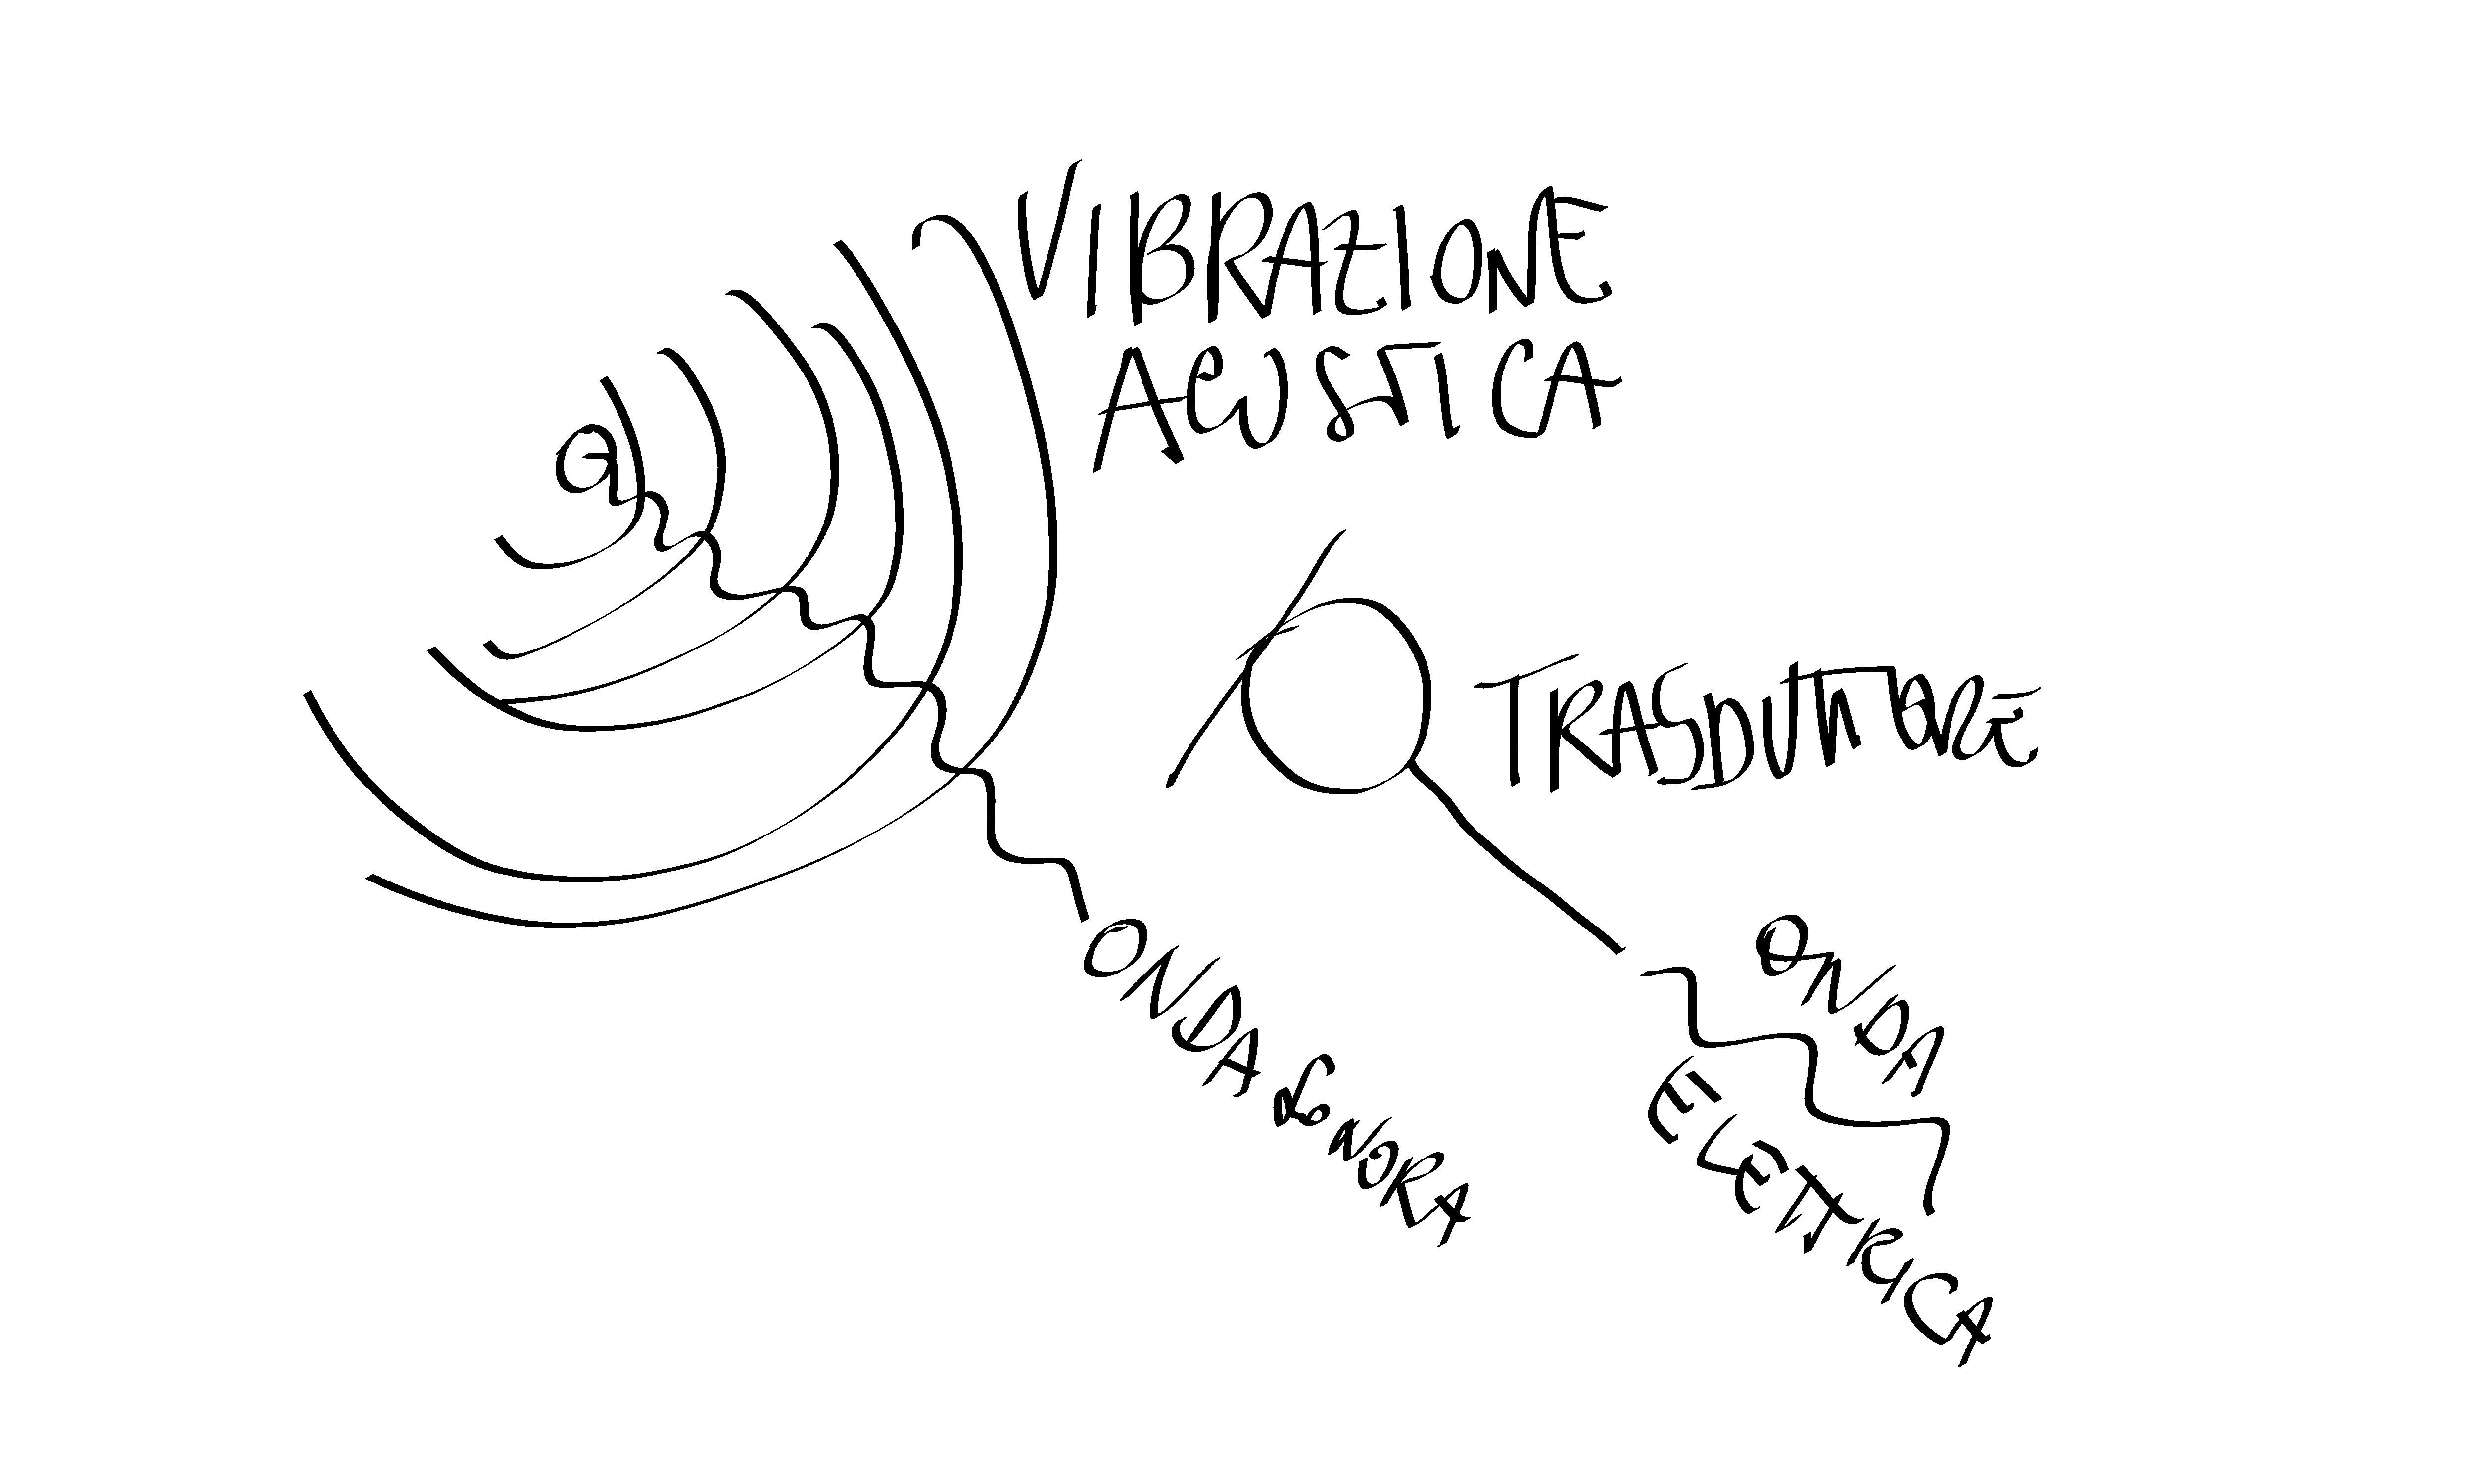
\includegraphics[width=0.99\columnwidth]{CAPITOLI/0200/img/trasduzione.png}
\caption[]{Generalizzazione di un sistema microfonico.}
\label{mic:condensatore}
\end{figure}

La generalizzazione del un microfono consiste in un sistema meccanico mobile esposto
all’onda sonora e destinato ad operare la \emph{trasduzione}\footnote{La
trasformazione della natura di un segnale operata da un trasduttóre,
derivato dall'inglese \emph{transducer} (che opera una trasduzione), dal latino
\emph{trans-ducere} (tras-portare). Il termine indica un dispositivo che converte
un segnale di data natura (acustica, elettrica, meccanica, termica, ecc.) in un
segnale di natura diversa. Si usa qualificare i t. con un aggettivo composto,
di cui la prima parte precisa la natura del segnale applicata e la seconda
parte quella del segnale d'uscita: t. acustoelettrico, che converte un suono in
un segnale elettrico (per es., un microfono), t. elettroacustico, da segnale
elettrico a suono (per es., un altoparlante). \\ – Fonte: Enciclopedia Treccani}
di una grandezza acustica, come la variazione di pressione, attraverso l'analogo
movimento meccanico rappresentato dallo spostamento della parte mobile del microfono, e da un sistema
elettrico a esso collegato destinato a operare la \emph{trasduzione} della
grandezza meccanica in una grandezza elettrica generando una una variazione di
corrente.

Tutti i microfoni si attivano attraverso una specifica amplificazione elettrica,
motivo per cui potremmo dire che li alimentiamo per copiare il campo sonoro
piuttosto che prenderne energia, sottolineando la peculiarità dell'osservazione
fisica: copiare il campo sonoro, intralciandolo.

Prima di procedere con una moderna classificazione dei microfoni, se ne può tracciare
brevemente il percorso storico.

Non si è stati bambini fortunati senza il \emph{gioco del telefono}. Muovere
un messaggio sottovoce tra file di orecchie e bocche allo scopo di tras-portare
l'informazione, sperando che questa venga tras-figurata, tra le risate. Più
felici di così solo con l'esperimento di collegare tra loro due bicchieri di carta con
uno spago per parlarsi, sottovoce, a breve distanza. È il suono mobile, nel tempo
e nello spazio, il meccanismo del suono in viaggio, che ha reso tutto possibile.

\begin{figure}[th!]
\centering
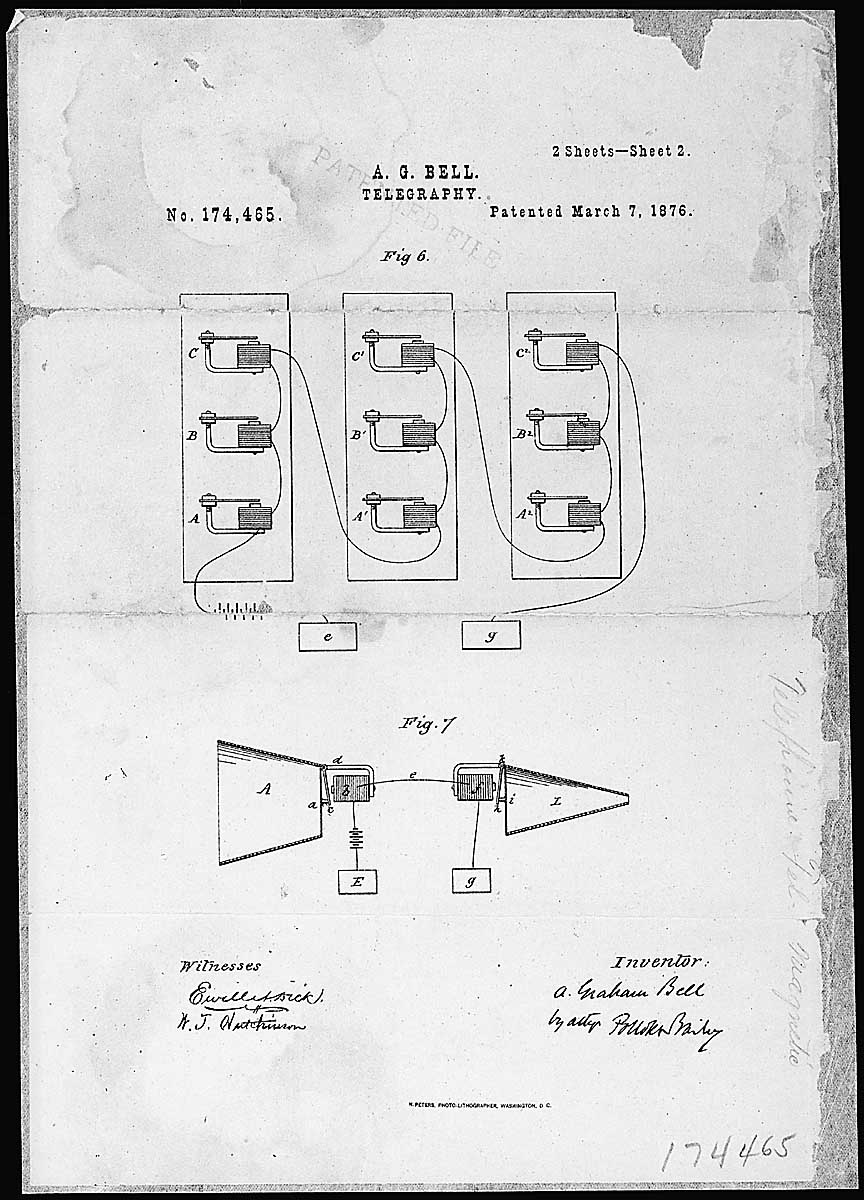
\includegraphics[width=0.99\columnwidth]{CAPITOLI/0200/img/telephone-patent-drawing-l.jpg}
\caption[]{Alexander Graham Bell.\\ Telefono. Registro brevetti: 302052.}
\label{agb:tel}
\end{figure}

Nel 1876, a Philadelphia, si teneva la \emph{Centennial Exhibition} per celebrare
il centenario della nascita della nazione. Fu la prima fiera mondiale a tenersi
negli Stati Uniti con lo scopo, tra gli altri, di annunciare a tutti che la nazione era
ufficialmente una potenza industriale. All'interno degli edifici della fiera erano
esposte le opere di due inventori: Alexander Graham Bell e Thomas Alva Edison.

\begin{figure}[th!]
\centering
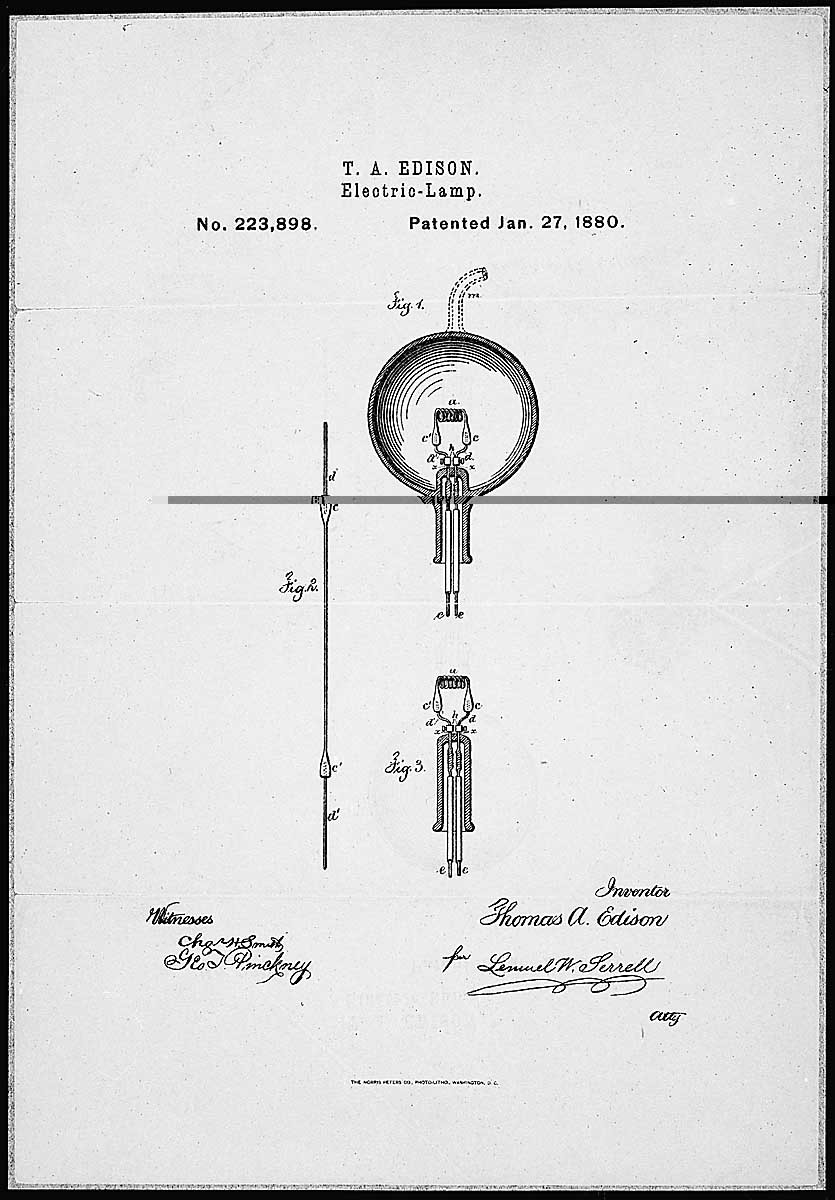
\includegraphics[width=0.99\columnwidth]{CAPITOLI/0200/img/light-patent-drawing-l.png}
\caption[]{Thomas Edison. \\ Lampada elettrica. Registro brevetti: 302053.}
\label{te:lamp}
\end{figure}

Un passo intermedio nello sviluppo della modulazione senza contatto (in aria) della
corrente continua è stato sviluppato nel 1878 da David Edward Hughes. In questa
realizzazione delle barrette di carbonio fissate ai due estremi venivano messe in
vibrazione dalle onde sonore dando luogo a una fluttuazione abbastanza grande
della resistenza
di contatto tra l'asta di carbonio e i due punti di fissaggio. Questo tipo di
microfono fu impiegato da Clement Ader nel 1881 nella sua pioneristica trasmissione a due
canali dal teatro dell'Opera di Parigi al padiglione espositivo.
Fu Hughes, per inciso, a usare per primo il termine \emph{microfono}, applicato
ai dispositivi di questo tipo.

Furono le compagnie radio-televisive a spingere nello sviluppo di queste tecnologie,
fin dagli anni venti, per aumentare la qualità del suono elettroacustico ad
entrambi gli estremi della catena: microfoni ed altoparlanti.

La compagnia \emph{Western Electric}, il ramo produttivo della \emph{Bell Telephone},
rispondendo alle esigenze crescenti sviluppava sia microfoni elettrodinamici che
a condensatore.

\begin{figure}[t]
\centering
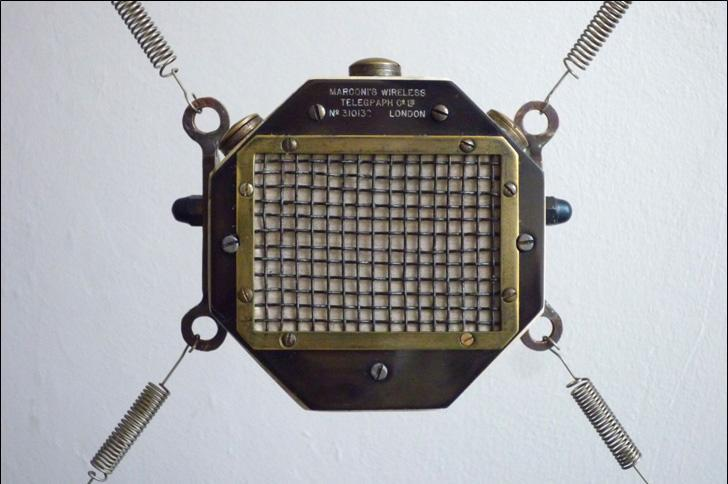
\includegraphics[width=0.99\columnwidth]{CAPITOLI/0200/img/1321872621718Reisz8.jpg}
\caption[]{Microfono \emph{Marconi-Reisz}, restauro RAI.}
\label{mic:Marconi-Reisz}
\end{figure}

Contemporaneamente in Europa Eugen Reisz stava cercando con George Neumann,
suo collaboratore, un nuovo sensore per avere un suono migliore rispetto al
microfono a dischi di carbone utilizzato nella telefonia. Le ricerche portarono alla
costruzione di un contenitore rettangolare fresato in un blocco di marmo o in
bachelite riempito di uno strato di finissimi granuli di carbone chiusi da un
diaframma non conduttore. L’involucro in marmo risulta privo di risonanze e la
cavità con i granuli di carbone è sigillata costituendo un \emph{microfono dinamico a pressione}.

Il microfono, progettato in Germania, è stato prodotto nel Regno Unito nel 1925/26
dalla \emph{Marconi Wireless}, motivo per cui è conosciuto come microfono
\emph{Marconi-Reisz} poi prodotto anche da \emph{AEG (Allgemeine Gesellschaft
Elektrik)} con piccole differenze costruttive.

Il microfono aveva una risposta in frequenza da $50Hz$ ai $1000Hz$ in modo
piuttosto lineare, estendendosi meno linearmente fino ai $10KHz$. Un microfono
di notevole qualità per quell’epoca, molto sensibile, che quindi veniva montato su un supporto elastico.

La risposta in frequenza poteva essere migliorata ulteriormente attravero un
circuito elettrico e qualche accorgimento operativo. Un'informativa interna
della \emph{BBC} del 1935 comunicava \emph{lo speaker deve
parlare attraverso il microfono ad un angolo di 45 gradi}, a sottolineare la relazione
tra dimensione del diaframma, angolo di incidenza e risposta in frequenza.
Le costruzioni successive portarono migliorie timbriche, nonostate alcune limitazioni
tra cui il livello di rumore di fondo abbastanza alto, causato dalle minuscole
scintille di scarica tra i granuli.
Un altro problema era che i granuli gravitavano verso il basso e
si compattavano. Questo produceva un livello di fruscio maggiore e una minore
sensibilità. Uno dei compiti dei tecnici audio dell’epoca era quello di passare
quotidianamente e prima di ogni programma negli studi e girare i microfoni
\emph{Reisz} a testa in giù e scuotendoli in modo da ridistribuire i granuli compattati.
Il manuale di Istruzioni del 1935 indicava che
il microfono doveva essere scollegato \emph{e, posto con il diaframma orizzontale
e rivolto verso l'alto\ldots} deve inoltre \emph{essere ben agitato da un lato all'altro in
modo da allentare il compattamento dei granuli}.

La sua uscita era comunque \emph{asimmetrica}, in quanto le onde di pressione
sonora comprimevano i granuli, ma la rarefazione non li decomprimeva.

\subsection{Architettura e principio di funzionamento}

Una prima catalogazione dei microfoni può essere effettuata per architettura,
ovvero in funzione delle caratteristiche costruttive che ne determinano i
risultati in termini di trasduzione.

In questa classificazione troviamo:

\begin{compactitem}
  \item microfoni dinamici
  \item microfoni a nastro
  \item microfoni a condensatore
  \item microfoni a condensatore electret
\end{compactitem}

\subsubsection{Microfoni dinamici}

Il microfono dinamico, indicato anche a bobina elettrodinamica,
elettromagnetica o mobile, si basa sul principio dell'induzione magnetica in cui
il conduttore, nel caso specifico l'avvolgimento di filo della bobina, si muove
attraverso un campo magnetico inducendo una tensione proporzionale alla forza
del campo magnetico, alla velocità del movimento e all'ampiezza del movimento
lungo il campo magnetico.

\begin{figure}[h]
\centering
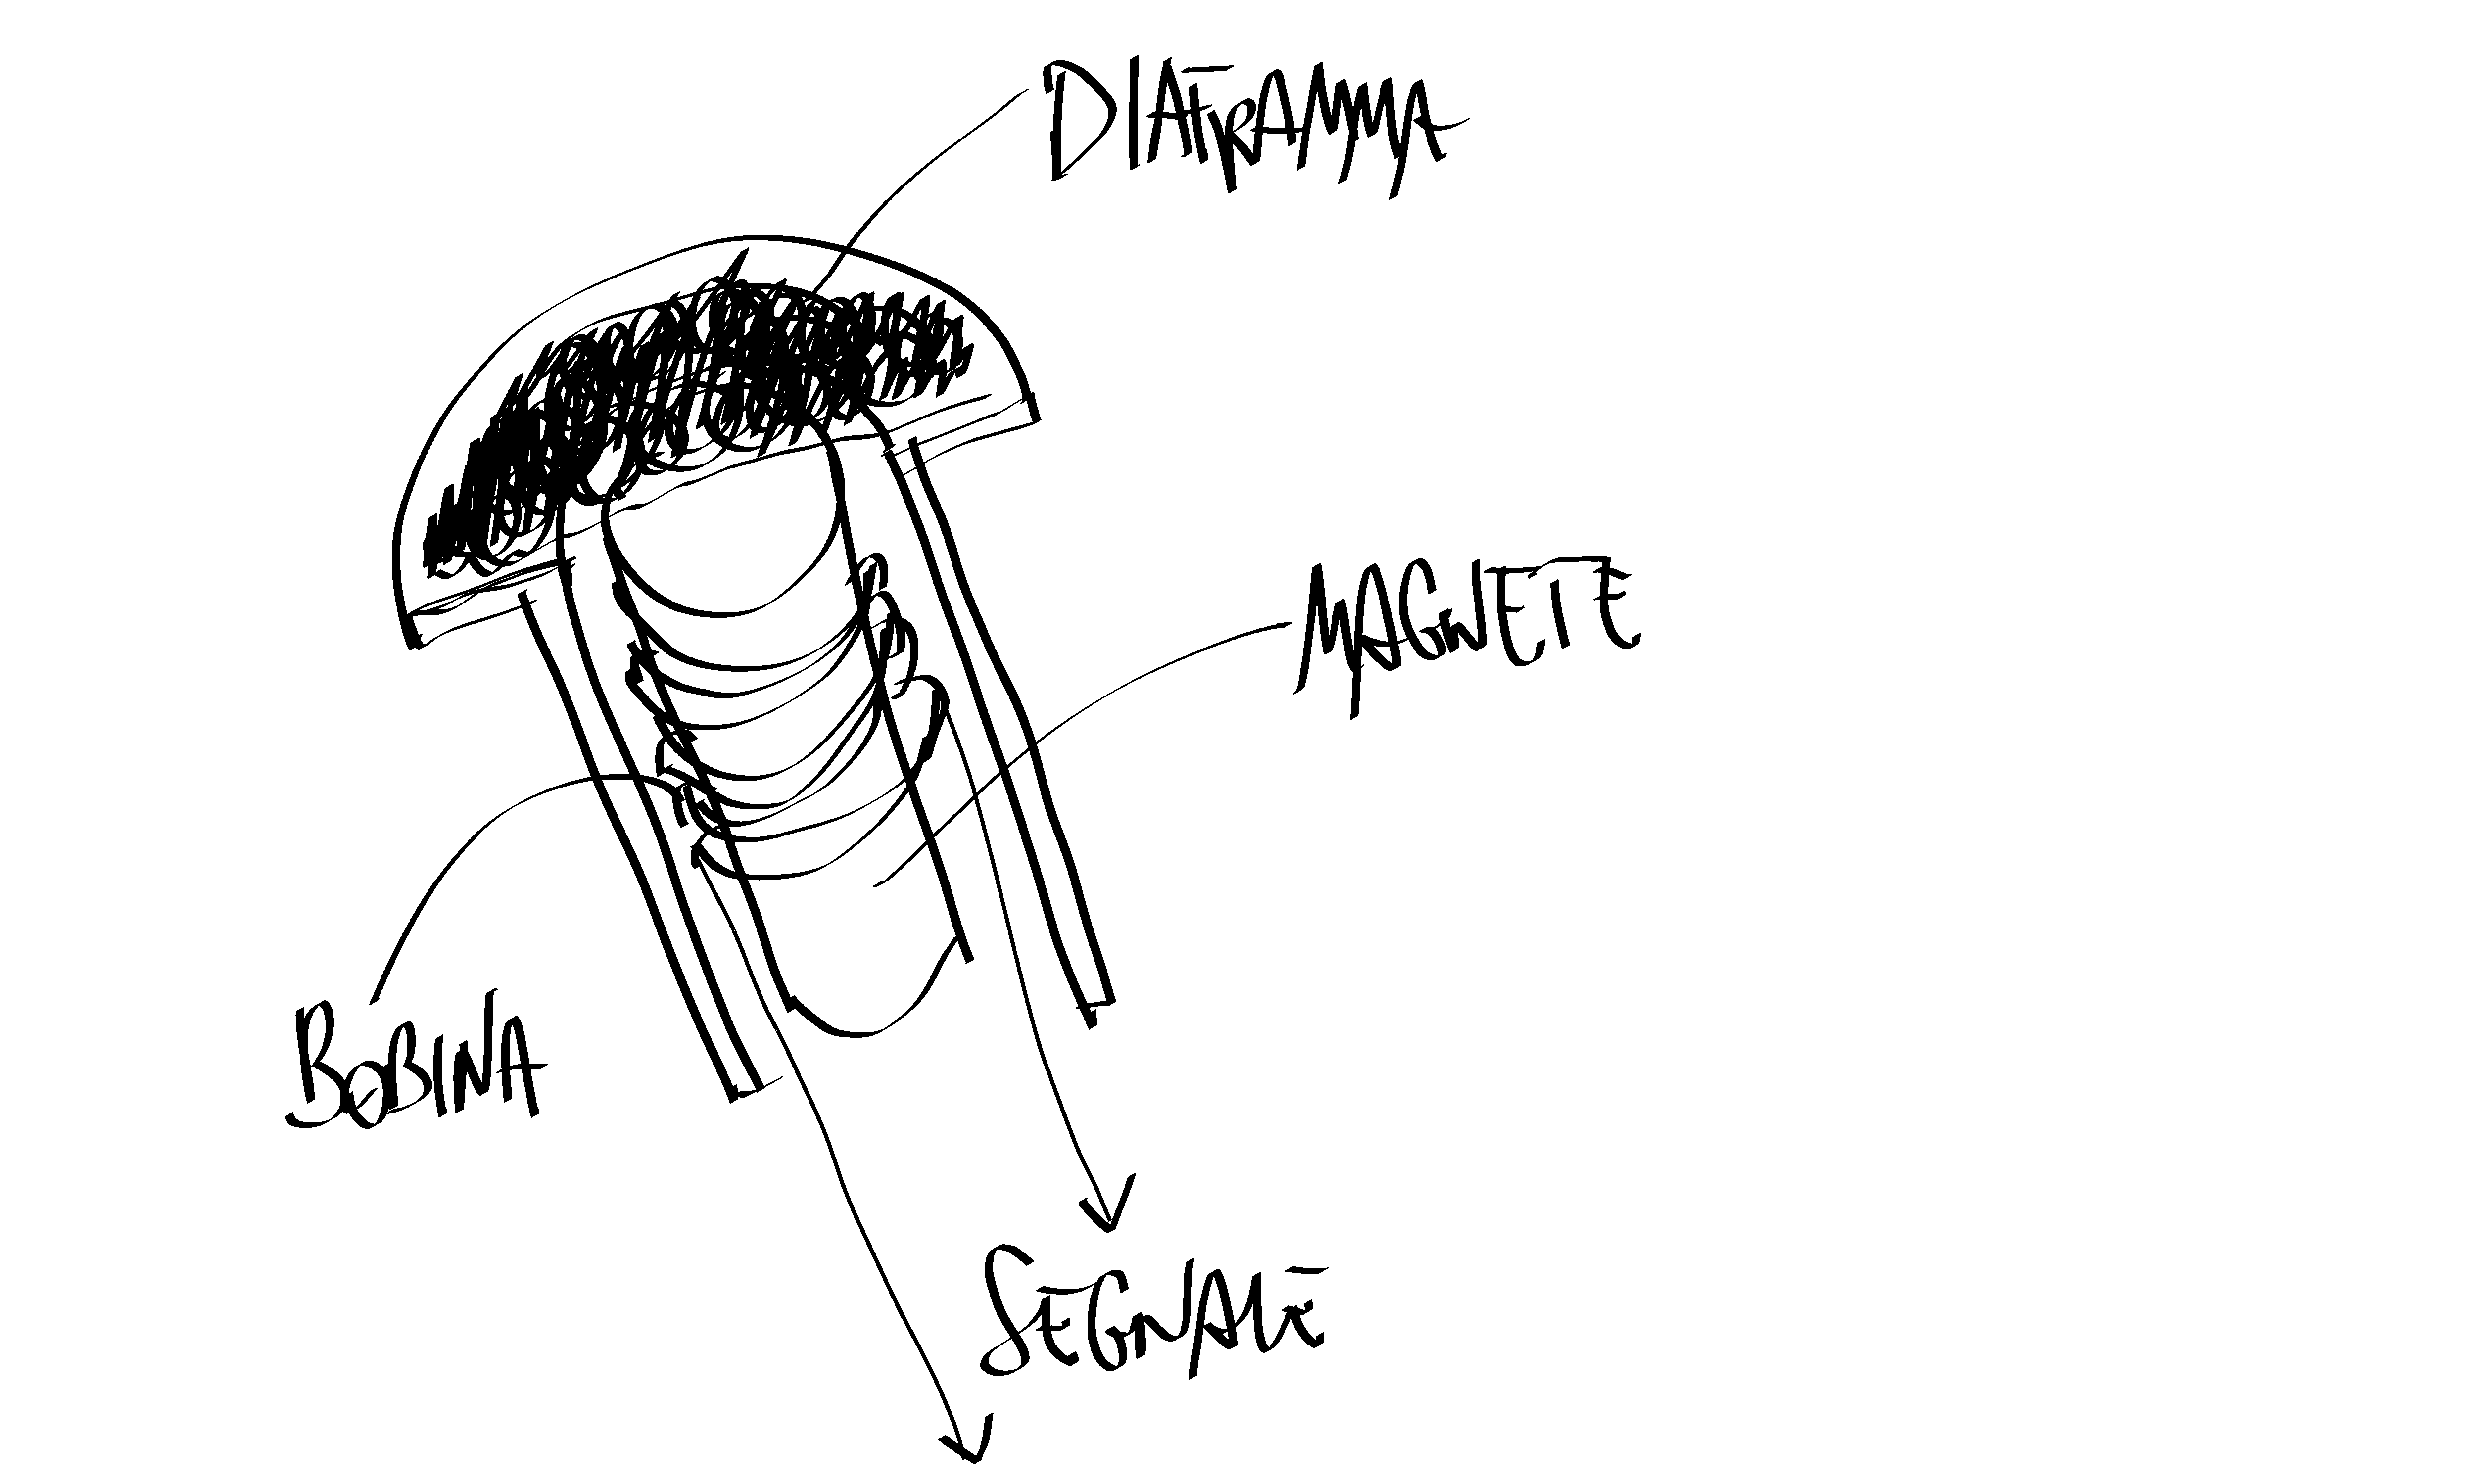
\includegraphics[width=0.99\columnwidth]{CAPITOLI/0200/img/mic-dinamic.png}
\caption[]{Microfono dinamico.}
\label{mic:dinamico}
\end{figure}

%A tale famiglia appartengono microfoni, la cui architettura è schematizzata in fig. 1,

Il diaframma circolare messo in vibrazione dalle onde sonore trasmesse nell’aria
è solidale con l'avvolgimento di filo di rame della bobina, libero di muoversi
all’interno di un campo magnetico costituito da un magnete permanente.

Le onde sonore, costituite da compressioni e rarefazioni dell’aria secondo una
determinata frequenza (corrispondente all’altezza del suono), vengono perciò
trasformate, attraverso tale trasduttore, in corrente elettrica, presente sui
cavi di uscita alle estremità dell’avvolgimento di rame, con variazioni di
ampiezza e frequenza analoghe a quelle delle onde acustiche. Questo
principio di trasduzione, come vedremo in seguito, non è altro che il
procedimento inverso a quello della maggior parte degli altoparlanti: in quel
caso, una corrente elettrica proveniente dall’amplificatore si presenta ai
poli estremi di una bobina mobile, anch’essa libera di muoversi all’interno di
un campo magnetico, e genera una corrispondente vibrazione sul cono
dell’altoparlante solidale alla bobina.

Le caratteristiche salienti di questo tipo di microfono sono:

\begin{compactitem}
  \item estrema robustezza ed affidabilità
  \item segnale di uscita molto basso
  \item risposta rimbrica limitata in banda
  \item scarso rapporto tra segnale e rumore
\end{compactitem}

È importante osservare come, a causa dell’elasticità e della massa del materiale
vibrante, il gruppo diaframma-bobina abbia una sua frequenza di risonanza
caratteristica. Al di sotto di tale frequenza il comportamento è dettato dal
rapporto elasticità/rigidità, mentre al di sopra dipende dalla massa del
complesso vibrante. Questo è uno dei motivi per cui i microfoni dinamici
tendono a \emph{colorare} il suono quando l'altezza in entrata si muove attorno
alla frequenza di risonanza, e tendono ad avere anche una risposta non perfettamente
estesa alle alte frequenze, a causa dell’inerzia delle masse in movimento.
Il rapporto tra qualità del segnale è proporzionale al numero degli avvolgimenti
della bobina, per cui il vantaggio della riduzione delle masse vibranti è
controbilanciato da un segnale di uscita inferiore, con conseguente diminuzione
del rapporto segnale/rumore. La soluzione risiede nel compromesso tra i valori
ottimali di tutti questi parametri.

L'evoluzione dei materiali nel campo dell'elettroacustica ha portato l'introduzione
nei sistemi dinamici (magnetici) del neodimio, utilizzato sia nei sistemi di
diffusione che di ripresa. La qualità del neodimio è nell'essere un materiale ad
alta coercitività, consentendo l’utilizzo di bobine a massa ridotta, a tutto
vantaggio della risposta alle alte frequenze.

\subsubsection{Microfoni a nastro}

In questo tipo di microfono il principio di funzionamento è assimilabile a
quello del microfono dinamico, con la differenza che la parte vibrante nonn è
costituita da un diaframma solidale ad una bobina mobile, bensì è costituito
da un sottilissimo foglio di alluminio
ondulato, anch’esso libero di vibrare tra i poli di un magnete permanente, e
alle estremità del quale si produce una tensione elettrica corrispondente alle
onde sonore in entrata. In questo tipo di microfono le funzioni
di vibrazione e di trasduzione sono svolte dallo stesso elemento fisico.

\begin{figure}[h]
\centering
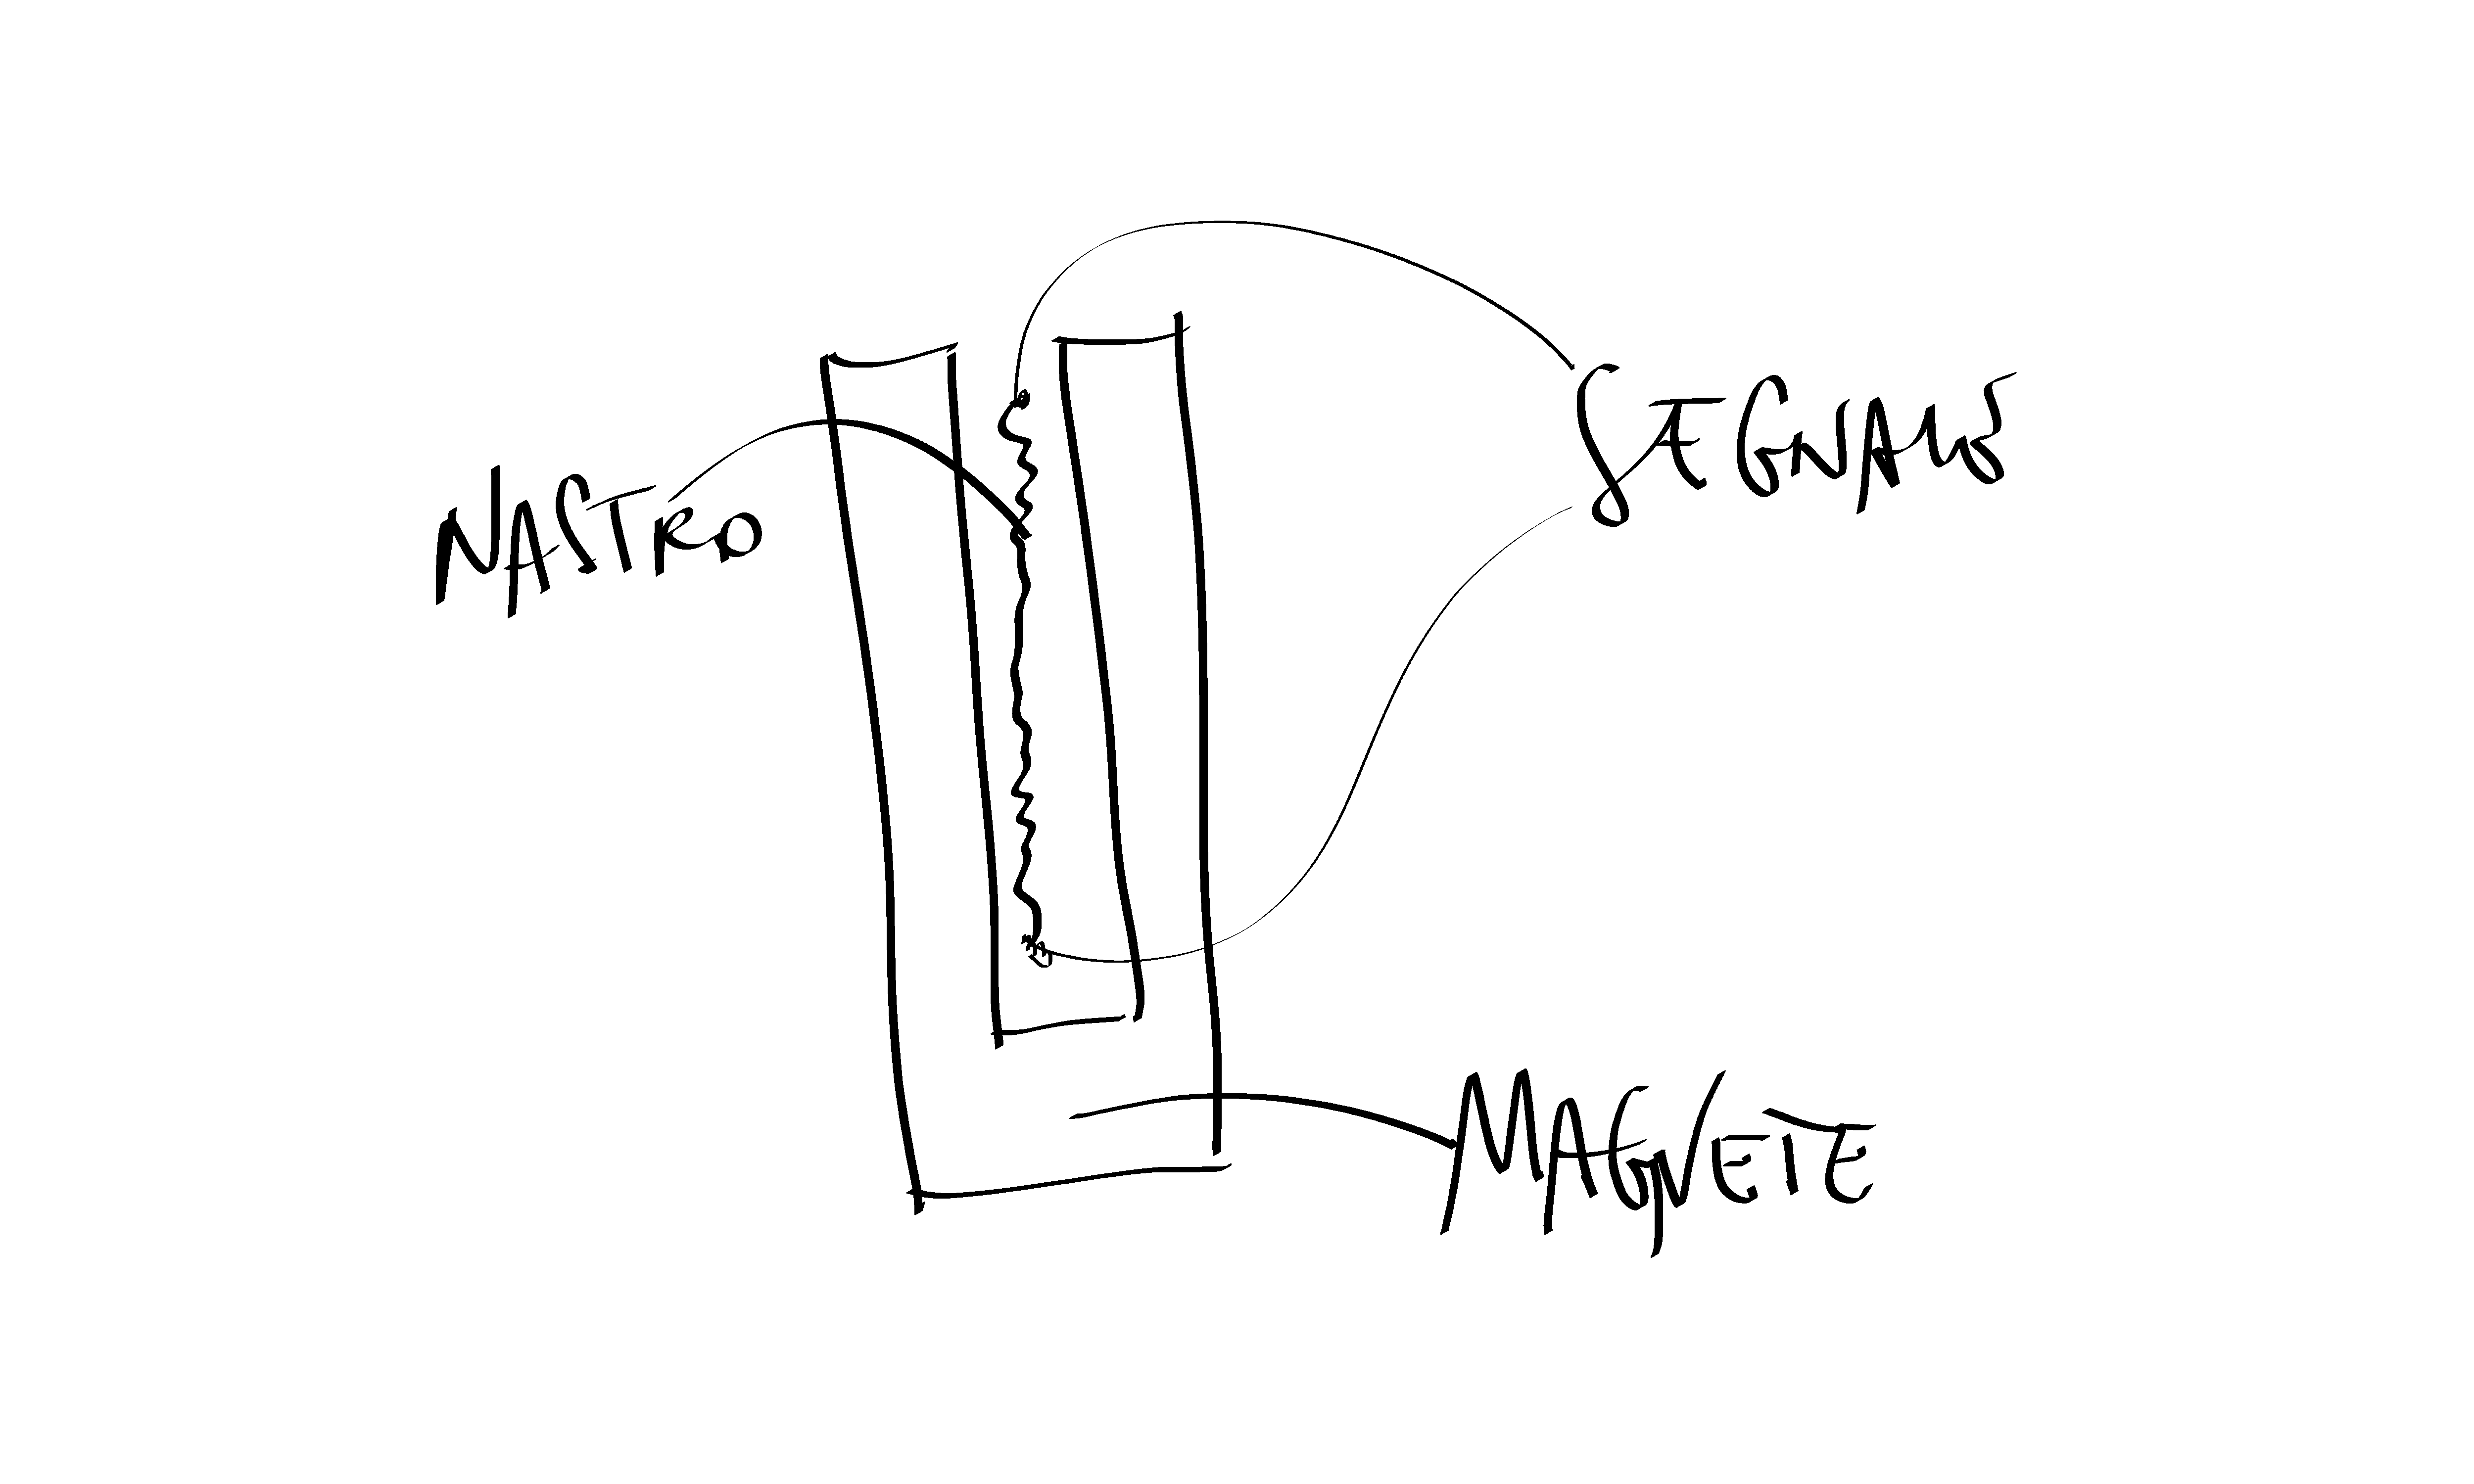
\includegraphics[width=0.99\columnwidth]{CAPITOLI/0200/img/mic-nastro.png}
\caption[]{Microfono a nastro.}
\label{mic:nastro}
\end{figure}

I primi microfoni a nastro erano piuttosto grandi, con magneti pesanti ed
inefficienti. Inoltre era piuttosto conosciuta la fragilità del nastro.

Le caratteristiche timbriche del microfono a nastro sono:

\begin{compactitem}
  \item assenza di coloratura dovuta alla frequenza di risonanza situata molto
  più in basso rispetto ai microfoni dinamici (inferiore ai $40Hz$);
  \item risposta estesa sulle alte frequenze a causa della ridotta massa del
  diaframma vibrante.
\end{compactitem}

Essendo il segnale d’uscita di livello estremamente basso,
ed essendo bassa anche l’impedenza di uscita, viene interposto un trasformatore
per elevarlo di intensità e fornire un’impedenza conforme allo standard.
La sottigliezza del nastro vibrante è inoltre causa di fragilità del dispositivo,
rendendolo inadatto alla microfonazione di segnali dotati di un’elevata pressione
sonora. Caratteristica di questo tipo di microfono è la naturale risposta bi-polare,
denominata figura-8, che sarà meglio descritta in seguito.

\subsubsection{Microfoni a condensatore}

Edward Christopher Wente iniziò a lavorare per la Western Electric nel 1914
sulla ricerca che prevedeva la progettazione e la calibrazione di un
trasmettitore (o microfono) uniformemente sensibile da utilizzare in laboratorio.
I microfoni a disco di carbone utilizzati nei ricevitori telefonici avevano una
risposta in frequenza troppo stretta, irregolare e un rumore di fondo eccessivo
per poter essere applicati nella ricerca sul suono. Con l'utilizzo
dell'amplificatore valvolare di Harold Dean Arnold, nel 1916, Wente produsse il
primo microfono a risposta in frequenza piatta da lui denominato trasmettitore a
condensatore. L'anno successivo pubblicò i suoi risultati in
un articolo teorico su \emph{The Physical Review}. Nel 1922, produsse un
trasmettitore a condensatore con una sensibilità cento volte maggiore, il che
era abbastanza per renderlo un dispositivo pratico, sebbene la sua alta
impedenza richiedesse il collegamento diretto ad un preamplificatore valvolare.

Il microfono a condensatore moderno è molto simile ai modelli originari di Wente
del 1917, solo molto più piccoli e raffinati nella costruzione. Spesso si fa
conusione nel riferirsi, in lingua inglese, a tale microfono attraverso il termine
\emph{condenser microphone}, tuttavia il termine rivela delle ambiguità e già
dagli anni venti del novecento ci si è riferiti alla tecnologia nei termini
di \emph{capacitor microphone}.

\begin{figure}[h]
\centering
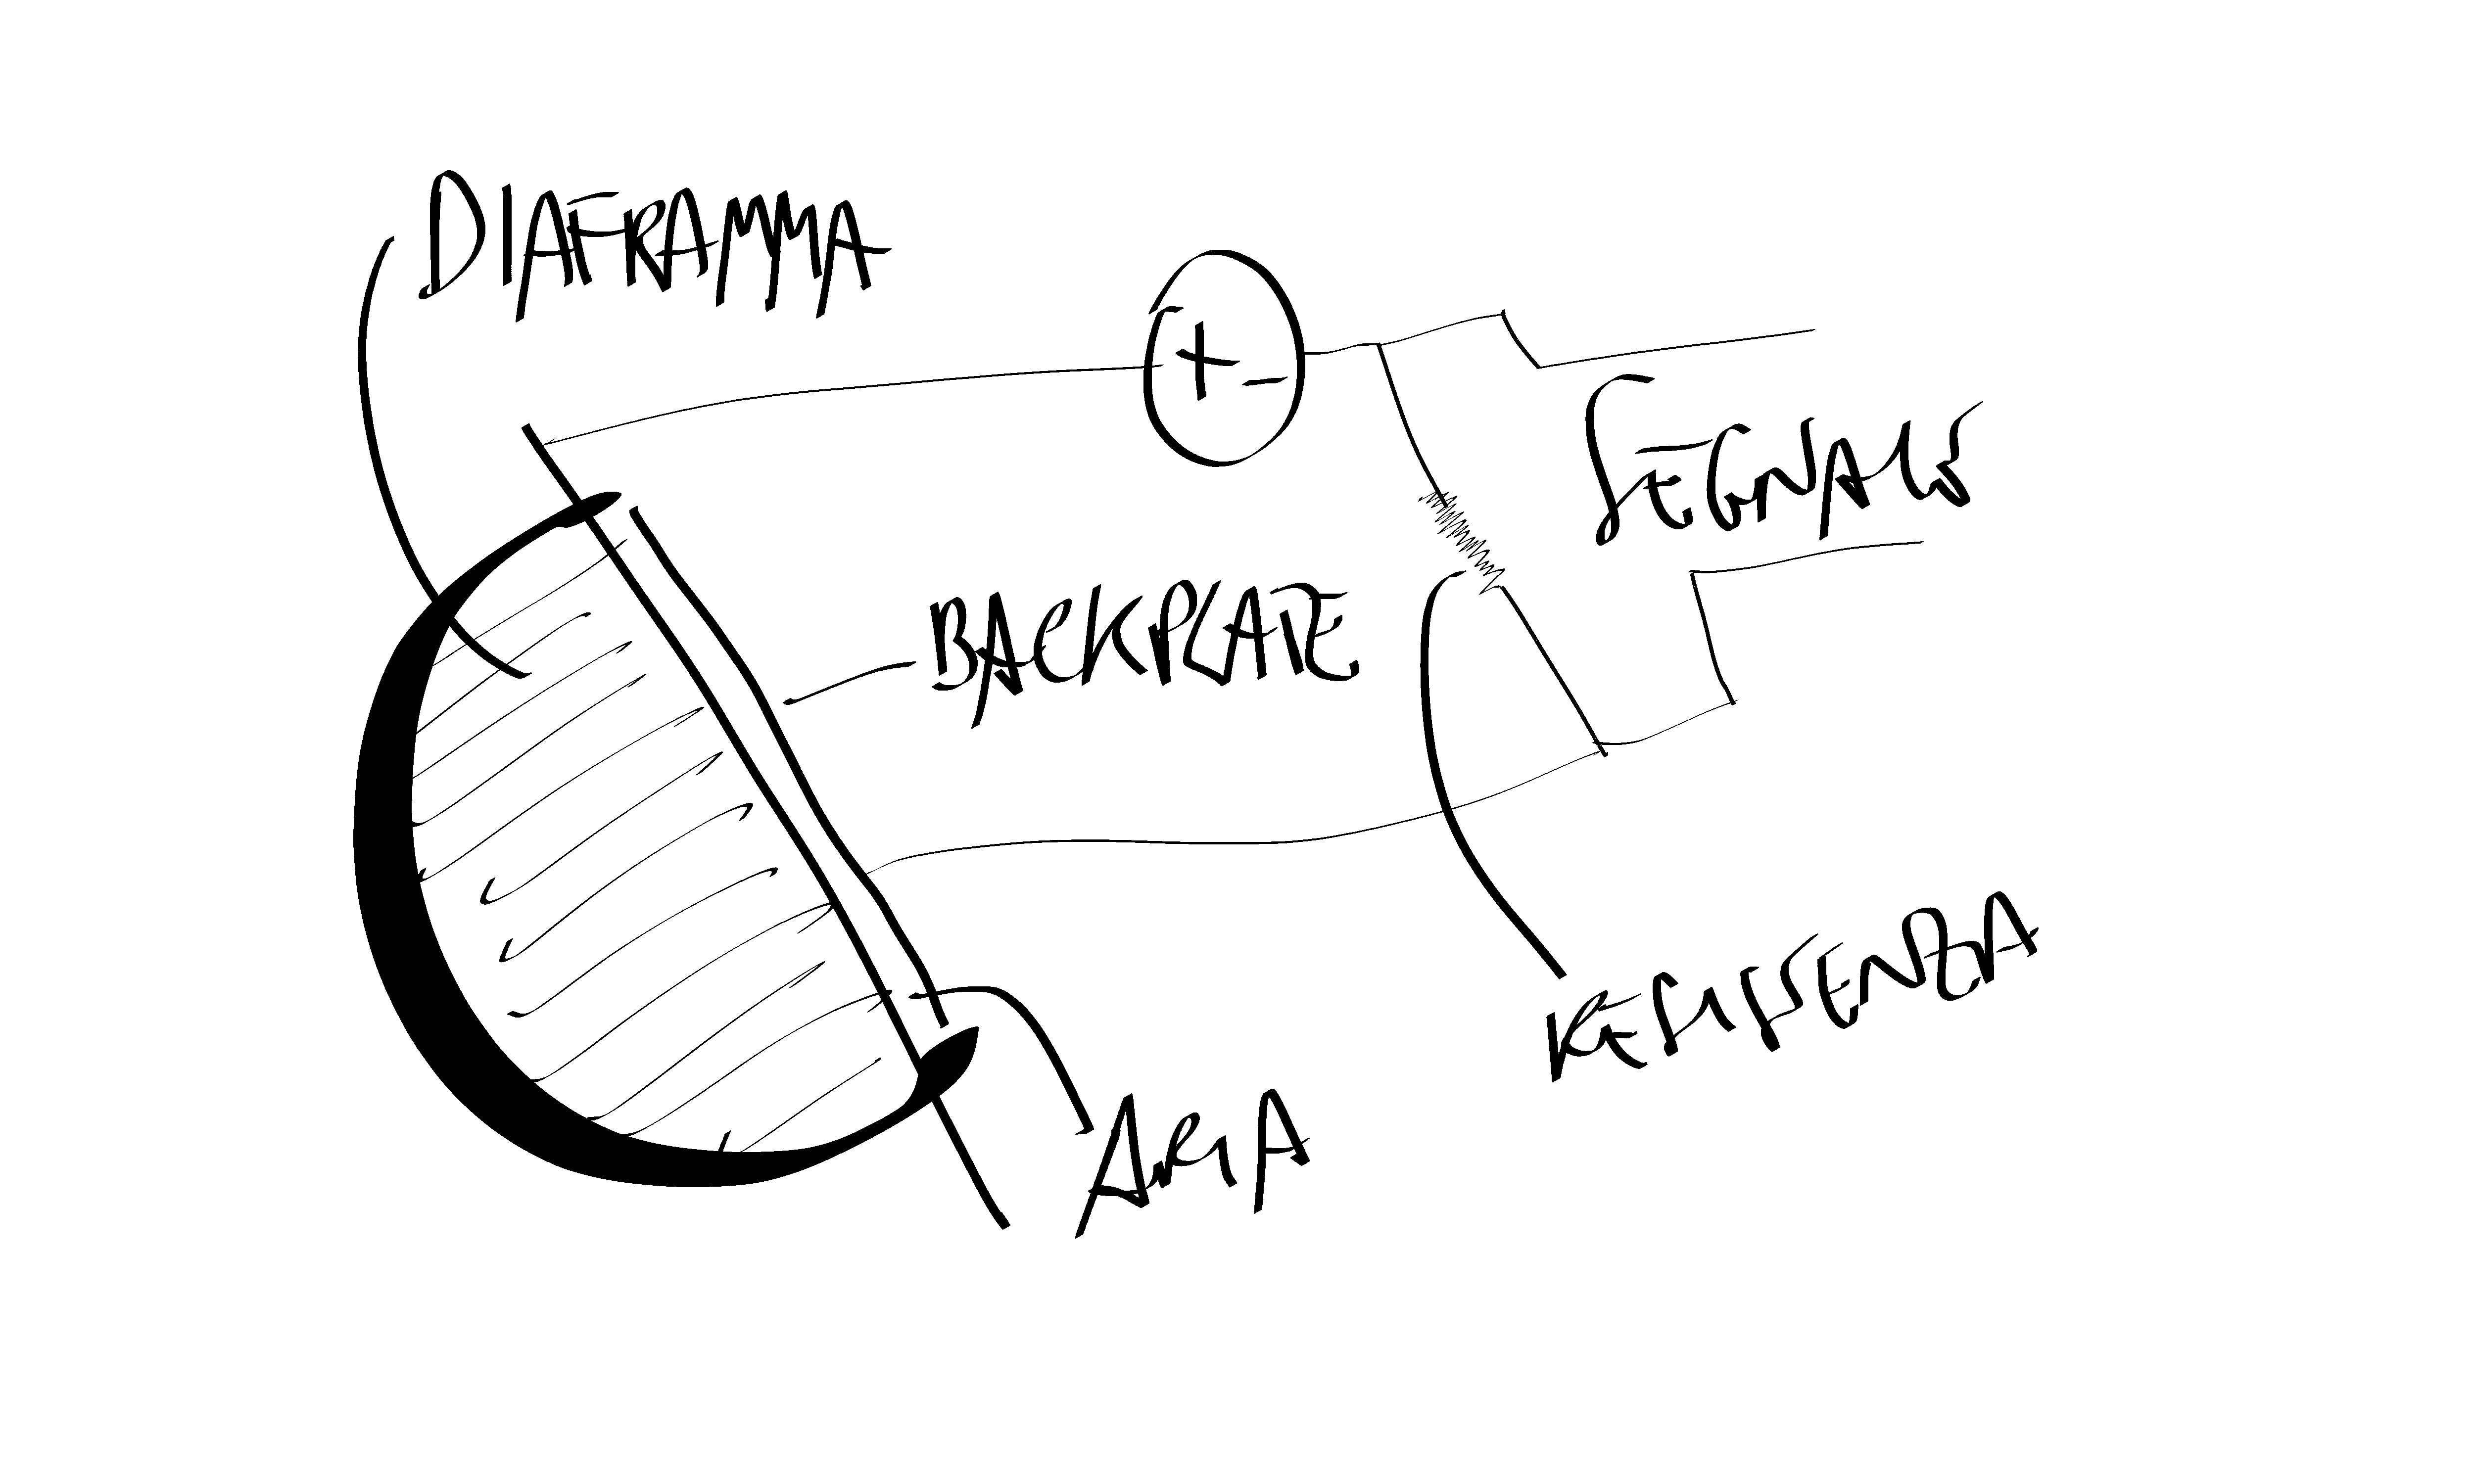
\includegraphics[width=0.99\columnwidth]{CAPITOLI/0200/img/mic-capacitor.png}
\caption[]{Microfono a condensatore.}
\label{mic:condensatore}
\end{figure}

Il microfono a condensatore è costituito da un diaframma (solitamente in materiale
plastico o metallico molto leggero come alluminio, nickel e titanio)
rivestito finemente d'oro. La lamina è distanziata da una seconda lamina fissa, più spessa,
denominata \emph{backplate} (lamina posteriore) che può essere forata. Le due
lamine hanno tra loro una differenza di potenziale in quanto
viene applicata una tensione di polarizzazione in corrente continua ad una delle
due.

\begin{figure}[tbhp]
\centering
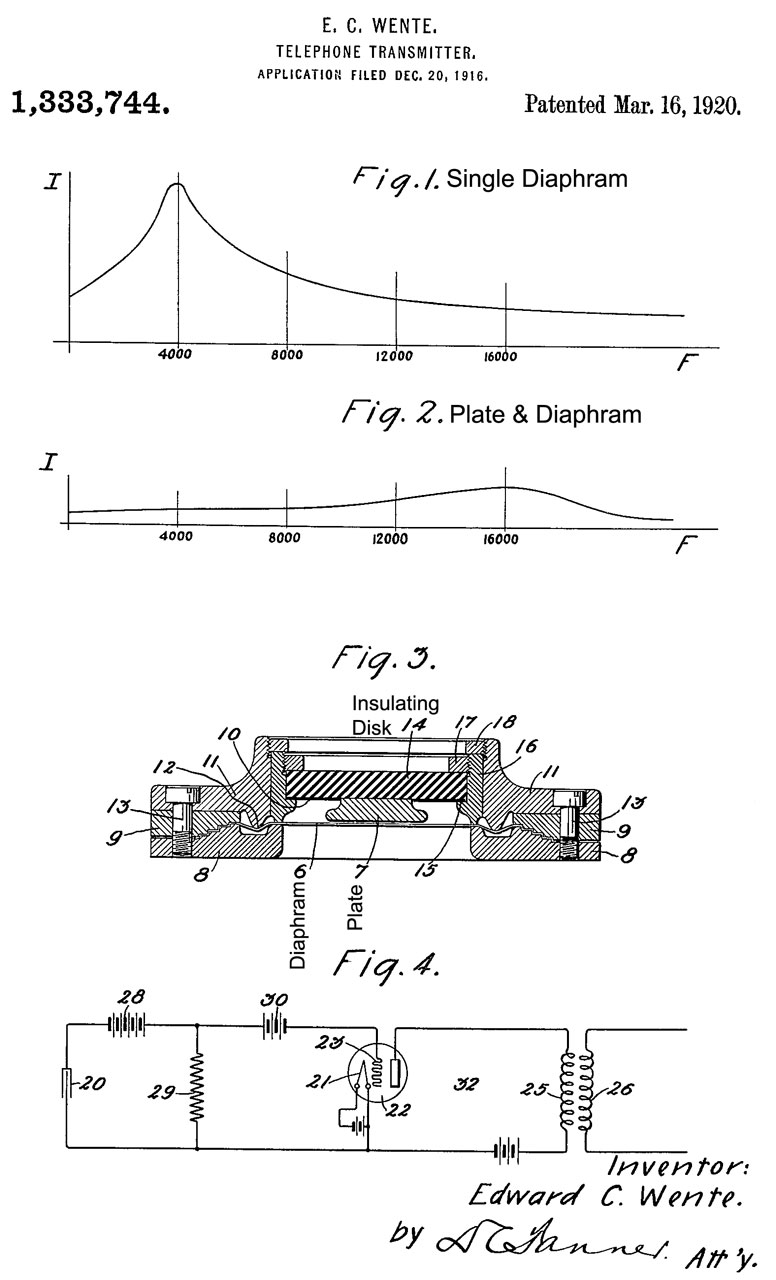
\includegraphics[width=0.99\columnwidth]{CAPITOLI/0200/img/US1333744-1b.jpg}
\caption[]{Edward Christopher Wente. \\ Microfono a condensatore. Registro brevetti: 1333744.}
\label{mic:wentemic}
\end{figure}

Il condensatore è un elemento elettronico passivo pre-polarizzato, in grado di
bloccare il passaggio di corrente alternata attraverso i conduttori tra i quali
è posizionato un diverso tipo di dielettrico. Quando esiste una differenza di
potenziale (tensione) tra i conduttori, viene generato un campo elettrico
statico che viene separato dal dielettrico tra cariche positive e negative
memorizzate rispettivamente sul polo positivo e negativo del condensatore.

Secondo il principio di funzionamento del condensatore, la vibrazione fa
quindi variare periodicamente la distanza tra le due lamine, generando una
corrispondente variazione periodica del campo elettrico e la conseguente
generazione di un’onda in uscita. Questa tecnica circuitale è nota come
“polarizzazione in corrente continua” (DC-biased), ed è differente da un’altra
tecnica, ossia la circuitazione RF (radiofrequenza). Quest’ultima prevede
un’oscillatore ad alta frequenza (in funzione di portante), rispetto al quale
il condensatore costituito dal corpo diaframma-backplate agisce in funzione
modulante. Il segnale verrà successivamente demodulato in bassa frequenza
restituendo il segnale elettrico originale. Il vantaggio di questo tipo di
circuitazione consiste in una riduzione del rumore di fondo generato dal
circuito di preamplificazione (inherent noise).

La circuitazione attiva all'interno di questo tipo di microfono necessita di
un'alimentazione esterna fornnita attraverso il sitema noto come alimentazione
fantasma (\emph{phantom power}), che consiste nel far viaggiare sul
cavo microfonico una determinata quantità di corrente continua. In alcuni casi
questa può essere fornita anche da dispositivi a batteria o da batterie interne
al corpo microfonico. Tale alimentazione consente inoltre di installare,
sempre all’interno del corpo microfono, un circuito di preamplificazione,
indispensabile, dato il bassissimo voltaggio generato dalle lamine, a fornire
un segnale d’uscita di livello adeguato.
In virtù di queste caratteristiche il microfono a condensatore offre:

\begin{compactitem}
  \item un segnale d'uscita efficace
  \item una curva di risposta in frequenza molto ampia
  \item elevata sensibilità
\end{compactitem}

Rispetto al microfono dinamico, offre un segnale d’uscita maggiore ed una migliore curva di
risposta in frequenza, contro una robustezza inferiore ed un costo decisamente superiore.

\subsubsection{Microfoni a electret}

La richiesta di tensione esterna necessaria alla polarizzazione del microfono a
condensatore ha rappresentato per molti hanni un ostacolo. In alcuni
contesti i grandi e pesanti preamplificatori potevano rappresentare uno svanntaggio
nella scelta del microfono. Agli inizi degli anni sessanta, presso i laboratori
Bell Telephone, Sessler e West descrissero un microfono a condensatore che utilizzava
materiale dielettrico permanentemente polarizzato, tra il diaframma mobile ed la
piastra posteriore (back-plate). I primissimi materiali utilizzati persero
sensibilità nel tempo, ma lo sviluppo di quella tecnologia ha portato risultati
ora molto stabili e paragonabili a quelli dei tradizionali microfoni a condensatore.

\begin{figure}[h]
\centering
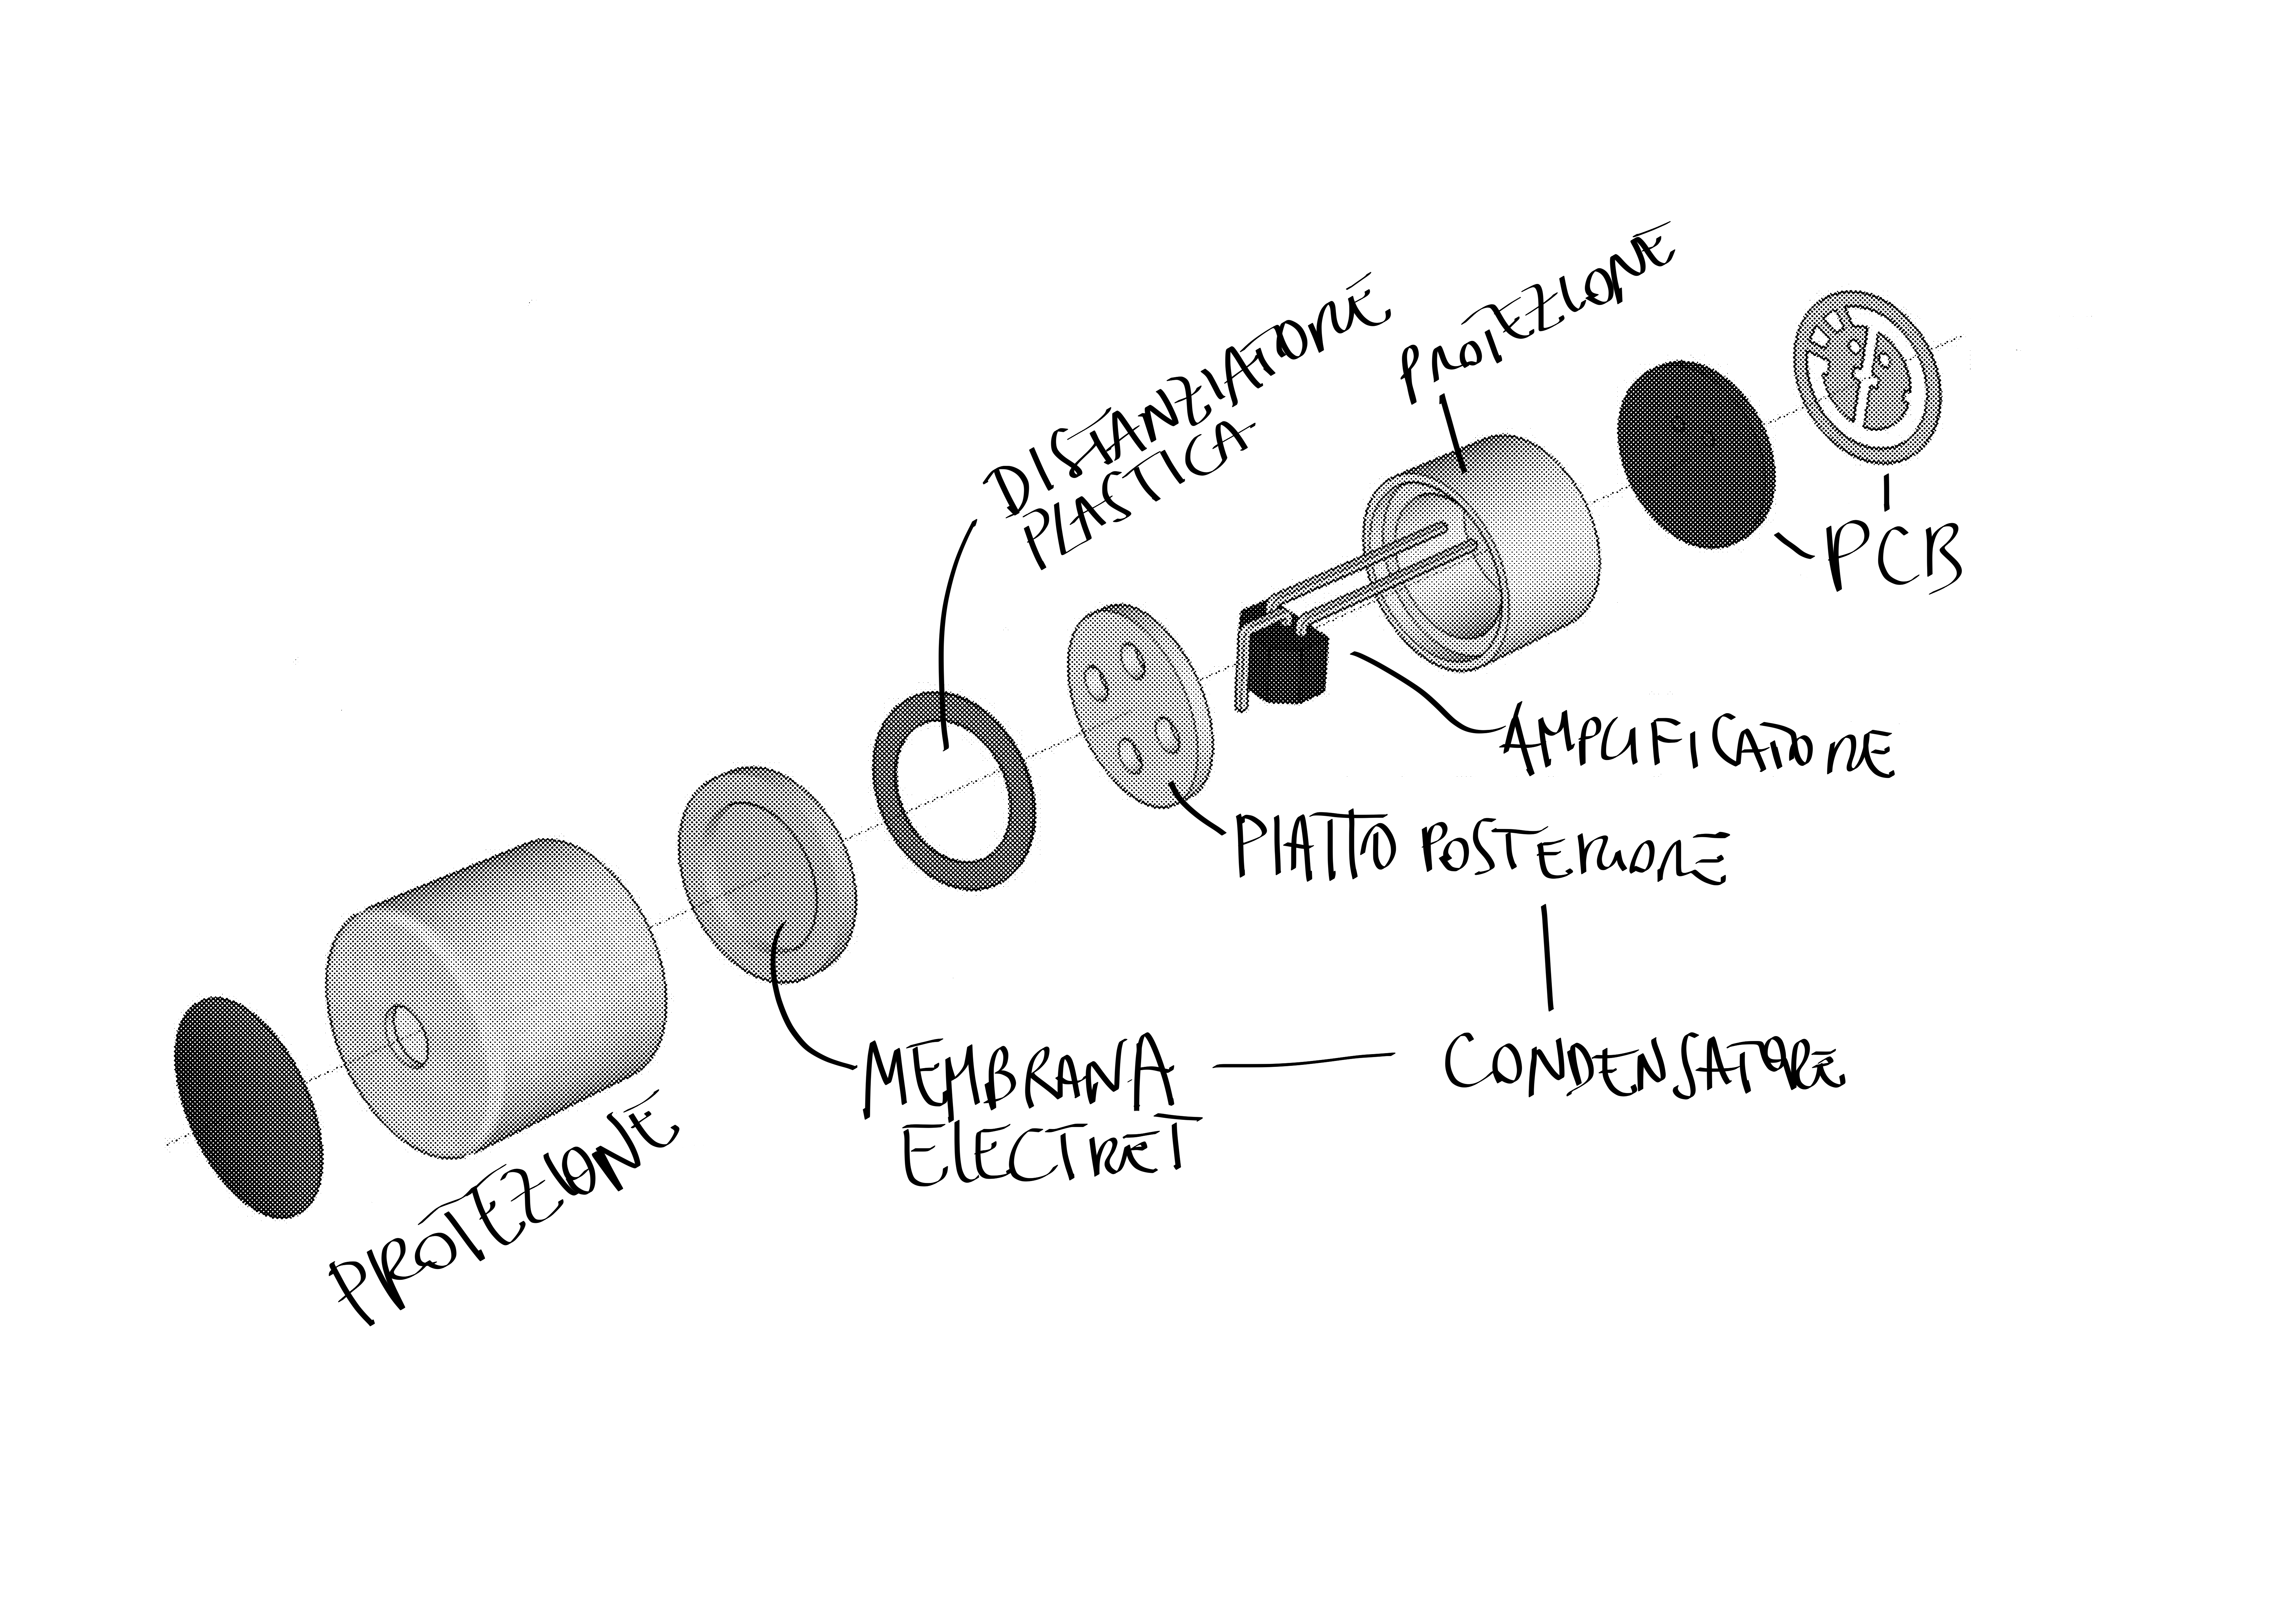
\includegraphics[width=0.99\columnwidth]{CAPITOLI/0200/img/electret.png}
\caption[]{Microfono a condensatore electret.}
\label{mic:electret}
\end{figure}

Il microfono a condensatore di tipologia \emph{electret} è quindi a tutti gli effetti
considerabile una variante nel campo dei microfoni a condensatore (\emph{ECM,
Electret Condenser Microphone}). La particolarità di questi microfoni è che tra
il diaframma e il backplate è inserito un dielettrico di materiale isolante
(electret) il quale ha la caratteristica di essere pre-polarizzato
elettricamente, in modo simile ad un magnete permanente nel campo del magnetismo.
In tal modo, il diaframma non necessita della tensione di polarizzazione,
sebbene questi microfoni siano comunque dotati di un circuito di preamplificazione,
per cui possono essere alimentati da alimentazione fantasma molto bassa o da batteria.
Sebbene questa tecnica sia sorta con l’intento di abbassare i costi, e
quindi sia stata implementata in prodotti economici rivolti più alle registrazioni
amatoriali che a quelle professionali, i progressi effettuati la collocano ormai
quasi alla pari con i migliori microfoni a condensatore. Tra i microfoni electret
i migliori sono da considerarsi quelli dove il dielettrico è solidale con il
backplate, che ne costituisce una delle superfici: essi prendono il nome di
\emph{back-electret}.

% Nella fig. 4 vediamo lo schema in sezione di un microfono electret, e possiamo
% notare come l’esiguità dei componenti lo rendano un dispositivo estremamente
% adatto alla miniaturizzazione, quindi adatto, ad es., ai microfoni a clip.

% \subsubsection{Parametri elettrici}
%
% A chiusura di questa panoramica sull’architettura dei microfoni occorre fornire
% qualche elemento sui parametri elettrici forniti a corredo dei microfoni. Oltre
% alle caratteristiche polari, di cui si parlerà di seguito, i valori più
% significativi per la valutazione di un microfono “sulla carta” sono:
%
% 1) La sensibilità
% 2) Il rumore
% 3) L ’impedenza
% 4) La risposta in frequenza
%
% La sensibilità indica il livello di segnale elettrico che il microfono pu
% fornire a fronte di una determinata pressione acustica sonora. Questo parametro
% ci fornisce un’indicazione utile per determinare quanto il segnale che il
% microfono produce dovrà essere amplificato negli stadi successivi. Così ad es.
% un microfono dinamico può fornire la seguente indicazione di sensibilità:
%
% 2 mV/Pa
%
% ossia 2 millivolt per una pressione acustica sonora di 1 Pascal2. Diamo di seguito,
% indicativamente, una tabella comparativa delle tipologie di microfoni presi in esame:
%
% Il parametro per valutare il rumore introdotto da un microfono è noto come
% “Equivalent Noise Level” (anche “self-noise level”, ossia il rumore inerente
% al microfono), e si riferisce ad un livello di pressione sonora che corrisponde
% al rumore interno del microfono, ossia al suono di livello minimo che è
% possibile registrare con un dato microfono. La scala di misurazione è quella
% del dBSPL , che sarà trattato in altra lezione, ed i metodi di misura sono
% generalmente di due tipi, in base alla curva di pesatura che viene applicata:
% 1) la scala dB(A), complementare delle curve isofoniche di Fletcher-Munson,
% mediante la quale i valori ottimali per i microfoni sono quelli al di sotto di
% 15 dB;
% 2) la scala CCIR 468-1, anche nota come ITU-R 468, che differisce dalla curva
% (A) per una maggiore enfasi nella zona da 5KHz a 8KHz, che fornisce valori
% ottimali al di sotto di 25-30 dB.
%
% In fig. 5 possiamo confrontare le due curve.
%
% L’impedenza del microfono (vedi fig. 6), di cui abbiamo già trattato,
% rappresenta quel valore resistivo che viene “visto” dall’apparecchio collegato
% in successione (preamplificatore, mixer, ecc.).
%
% Come si può osservare in tab. 2, il valore tipico dei microfoni professionali
% è di 200 Ohms, ma con oscillazioni che possono andare da 50 a 600 Ohms.
%
% Risposta in frequenza
%
% Vi sono diversi modi di rappresentare il comportamento di un microfono rispetto
% alle frequenze dei suoni in entrata e rispetto all’angolo d’incidenza degli stessi.
% Uno di questi, la curva di risposta in frequenza, rappresentato in fig. 7, è un
% grafico dove i parametri sono dati dall’ampiezza del suono (sull’asse verticale)
% e dalla sua frequenza (sull’asse orizzontale), e dove i diversi angoli, ch
% rappresentano la quantificazione dello scostamento della provenienza del suono
% rispetto all’asse, sono rappresentati da una famiglia di curve, in cui ad ogni
% curva è associato un valore angolare.
%
%   Curve polari
%
% Il diagramma polare (o curva polare) è invece un grafico a disegno circolare dove i parametri sono dati dall’ampiezza e dall’angolo d’incidenza, mentre le frequenze sono rappresentate da famiglie di curve. In presenza di un’unica curva, si intende che questa è riferita ad una frequenza di 1 KHz.
% Il disegno nella parte sinistra di fig. 8 rappresenta la struttura di un tipico microfono a pressione (pressure microphone) omnidirezionale, mentre nella parte destra è rappresentata la sua curva polare, dove vediamo che la direzionalità del suono inizia ad essere percepita dal microfono a partire da circa 5 KHz in su, mentre le frequenze gravi non sono indicate in quanto assimilabili a quella rilevata a 1 KHz, cioè con attenuazione zero per qualsiasi angolo di provenienza del suono.
%
% Per comprendere il principio di funzionamento di un microfono a pressione dobbiamo immaginare il diaframma di un microfono, sia esso dinamico o a condensatore, come la pelle di un tamburo tesa sopra un contenitore ermeticamente chiuso (backchamber, in figura) Avremo quindi un dispositivo che oscilla in presenza di variazioni di pressione provenienti esclusivamente dall’esterno, essendo la parte interna a pressione costante. Tale trasduttore è per questo motivo chiamato microfono a pressione, ed essendo le variazioni di pressione indipendenti dall’angolo di arrivo delle stesse, la caratteristica polare fa di questo dispositivo un microfono omnidirezionale.
% La possibilità di reagire in modo uniforme ad ogni direzione di provenienza del suono è in realtà teorica, come si può perfettamente osservare guardando la sua curva polare, in quanto per il principio della diffrazione acustica le frequenze della gamma alta tenderanno ad attenuarsi al crescere dell’angolo di incidenza a partire dall’asse del microfono, mentre tenderanno ad elevarsi al diminuire dello stesso angolo di incidenza, ossia man mano che l’angolo di arrivo va a coincidere con l’asse. Il fenomeno è dovuto
%
% alla presenza fisica del microfono stesso nel campo sonoro che interferisce con la propagazione delle onde sonore. Un microfono che, per la sua costruzione fisica, dovuta essenzialmente al ridotto diametro del diaframma, sia esente da questo fenomeno è detto microfono a campo libero (free-field microphone). Un microfono a pressione può lavorare come microfono a campo libero nel momento in cui gli venga applicata una correzione acustica e/o una equalizzazione (free-field correction) che rendano il suo comportamento lineare alle frequenze alte.
% La caratteristica di esaltazione delle frequenze alte in asse è stata, nel corso della storia, sfruttata al fine di ottenere la linearità che si perde naturalmente con la distanza per via della densità dell’aria, che tende a penalizzare proprio le frequenze alte. Nella fig. 9 vediamo un esempio di applicazione di sfruttamento del fenomeno col microfono Neumann M50, in cui il diaframma è incastonato in una forma sferica, con l’intento di interferire maggiormente col campo libero. Nella parte destra vediamo la sua curva caratteristica, che lo hanno reso una scelta preferita nelle riprese panoramiche di orchestre.
%
% Nella fig. 10 abbiamo la rappresentazione di una curva sensibilmente differente dalla prima, in quanto vediamo che l’attenuazione del segnale ha il suo punto massimo a 180° (alle spalle del microfono), ed è già significativa (circa 12 dB) a 500 Hz. Tale curva polare descrive il comportamento di un microfono direttivo noto come microfono cardioide. Il termine
%
%
% “cardioide” deriva dalla forma a “cuore rovesciato” che tende ad assumere la curva polare.
%
% E’ importante evidenziare che la direzionalità del microfono è ottenuta mediante l’apertura, alle spalle del diaframma, di fessure la cui funzione è di far pervenire parte del suono sul retro del diaframma, generando un’opposizione di fase in grado di agire sui suoni laterali e posteriori, come illustrato in fig. 11.
% In conseguenza del fatto che il diaframma è aperto nella zona retrostante, il microfono è detto microfono a gradiente di pressione (pressure gradient microphone), in quanto la sua risposta è generata dal rapporto della pressione frontale con quella posteriore.
% Dal momento che il percorso che compie il suono in entrata alle fessure laterali è un percorso finito, mentre i suoni possono avere frequenze diverse, l’opposizione di fase è “accordata” sulle frequenze medio-alte per evidenziare la direttività. A causa di ciò esiste un effetto collaterale derivante da questa tecnica, consistente nel fatto che, nel momento in cui il microfono direzionale è installato molto vicino alla fonte sonora, si genera un’esaltazione innaturale delle frequenze gravi, dovuta proprio alla presenza delle aperture laterali. Questo effetto, che può anche essere adoperato in modo appropriato per ottenere un suono particolarmente “caldo” ad es. nella voce, prende il nome di effetto di prossimità (proximity effect).
%
% Aumentando la lunghezza della zona del corpo microfono aperta da fessure, come nel microfono di fig. 12, si aumenta la caratteristica direzionale del microfono, la cui curva prende il nome di supercardioide. A causa della ridotta efficacia dell’accordatura laterale per i suoni a 180°, compare nella curva un lobo posteriore che sposta il punto di attenuazione massima dai 180° della curva cardioide a circa 135° (225° nel terzo quadrante). Nei microfoni a curva ipercardioide è ulteriormente ristretta l’angolazione frontale, mentre viene accentuata la caratteristica del lobo posteriore, rendendoli una soluzione intermedia tra la curva supercardioide e la curva a figura-8 di cui parleremo più avanti. Il punto di attenuazione massima è ora intorno a 110° (250° nel terzo quadrante), come illustrato in fig. 13.
%
% Tra i microfoni a gradiente di pressione, esistono infatti dei microfoni, detti a figura 8, la cui curva polare, illustrata in figura 14, presenta una simmetria avanti/dietro, dove i punti di attenuazione massima si vanno a situare a 90° e 270°. Tali microfoni hanno uguale sensibilità per i suoni provenienti dal fronte e dal retro, mentre tendono ad annullare i suoni di provenienza laterale. I microfoni a nastro di cui abbiamo parlato sono caratterizzati da tale curva.
%
% Per chiudere la panoramica delle curve polari è opportuno notare come esse possano venire espresse da funzioni trigonometriche, in modo da descrivere il valore punto per punto della curva partendo dall’angolo di incidenza del suono, come evidenziato in fig. 15.
%
% A completamento della panoramica sulle tecniche costruttive impiegate per ottenere la possibilità di variare la direzionalità del microfono è importante accennare ai microfoni a condensatore che si avvalgono di un doppio diaframma installato al loro interno. Nella fig. 16 notiamo come due diaframmi sono montati “spalla a spalla” (back-to back) con in mezzo il backplate. La combinazione di intensità e di fase delle due membrane può fornire una gamma di caratteristiche polari diverse, dalla omnidirezionale alla figura 8, fino alla cardioide e all’ipercardioide. Tale configurazione è nota anche come “Braunmühl/Weber” dai nomi dei suoi inventori (1937), e si avvale tipicamente di diaframmi a largo diametro, a differenza dei microfoni a pressione che per avere
% maggiore omnidirezionalità devono essere forniti di un diaframma di piccolo diametro.
%
% Per particolari situazioni in cui è richiesta poca intrusività visiva del dispositivo di ripresa sono adoperati dei microfoni, detti pressure zone microphones o anche boundary microphones, illustrati in fig. 17, la cui architettura consiste in una capsula omnidirezionale montata molto vicino ad una piastra piana, la quale a sua volta va utilizzata a
% contatto con una superficie (pavimento, muro, tavolo, ecc.). Il principio consiste nel fatto che, diversamente da quel che accade in un microfono tradizionale montato, ad es., su un’asta, il suono diretto dallo strumento non è degradato, per effetto di comb-filter, dalle riflessioni dell’ambiente circostante, ma, grazie a questo disegno, le onde sonore arrivano tutte egualmente riflesse dalla piastra verso la capsula, e quindi perfettamente in fase. In pratica la superficie d’appoggio agisce da barriera del suono, e il microfono è così in grado di captare il suono senza cancellazioni di fase dovute a riflessioni. La curva polare che tale microfono genera, in virtù del suo posizionamento su di una superficie, è così una curva emisferica, cioè una curva semi-omnidirezionale (half- omnidirectional) che si irradia “al di sopra” del microfono.
%
%
% Esistono infine dei microfoni, detti “parabolici”, schematizzati in fig. 18, che si avvalgono della proprietà acustica di una superficie paraboloide di concentrare per riflessione le onde sonore in un unico punto (fuoco della parabola) consentendo a dei normali microfoni di assumere delle caratteristiche di spiccata direttività, di molto superiore a quella fornita dai microfoni ipercardioidi. L ’utilizzo di tali microfoni è chiaramente limitato ad alcuni ambiti, come la ripresa a bordo campo di eventi sportivi, la cattura a grande distanza di suoni del mondo animale per scopi scientifici e documentari naturalistici, e le intercettazioni ambientali.
%
% Naturalmente, la risposta in frequenza di un tale dispositivo non potrà mai essere a banda piena, ma presenterà un’inevitabile carenza sulle basse frequenze, in quanto la parabola sarà in grado di
% riflettere solamente i suoni con lunghezza d’onda sensibilmente inferiore al valore del suo diametro.
% I vantaggi che può dare un tale dispositivo si possono verificare nella fig. 19: il microfono è tanto più efficiente quanto più largo è il diametro della parabola, fornendo un guadagno sul segnale che può arrivare a 30 dB a 8.000 Hz.

\printbibliography
\end{refsection}


\clearpage

%!TEX TS-program = xelatex
%!TEX encoding = UTF-8 Unicode
% !TEX root = ../../metm.tex

\section{Riproduzione}

JEAN CLAUDE RISSET SUONO TEMPO SUONO SPAZIO

L'esperienza sonora è viva nella produzione acustica del suono. Culturalmente
siamo portati a pensare che i nostri sistemi audio siano in grado di ricostruire
quella esperienze, senza mai minimamente pensare che questo è semplicemente e
praticamente impossibile. Ci sono diversi motivi culturali per cui lo pensiamo.
Ci sono innumerevoli questioni e parole consumate dalla pratica quotidiana.
Parole private del loro significato originale e consumante nella concezione di
una immotivata sicurezza operativa, come per esempio quella applicata al suono
stereo a due canali. Nell'esperienza quotidiana siamo divertiti e soddisfatti
dalla stereofonia, senza necessariamente mettere a confronnto o relazione con
quella che dovrebbe essere la vera esperienza. La semplice differenza tra i due
canali, destro e sinistro, è proposta come stereofonia. Altoparlante sinistro,
altoparlante destro. Centro? Fantasma. Raramente si sente descrivere questa
tipologia di ascolto come monofonica, mono o doppio mono, o polifonica. Una
soprgente di questo tipo ascoltato attraverso le cuffie diventa orecchio
sinistro, orecchio destro e centro della testa. Certamente può esserci
un'essenza di musica in tutto ciò, la persistenza i un segnale culturale. Manca
però in una riproduzione di questo tipo qualsiasi parvenza di spazio acustico e
atmosfera di realismo o verosomiglianza. La sapiente configurazione nella
ripresa microfonica e l'elaborazione del segnale operato  durante la
registrazione possono migliorare le cose, ma nella migliore delle ipotesi la
stereofonia così basata su due sorgenti di riproduzione rimane un formato
direzionalmente e spazialmente debole, privato, e antisociale, che può soddisfare
un solo punto di ascolto.

% Abbiamo bisogno di più canali per acquisire, archiviare e riprodurre anche le
% percezioni essenziali dei campi sonori tridimensionali. Questo è ciò che il
% mondo del cinema conosce da decenni, e ora i cinema hanno ben 62 canali nei
% formati audio coinvolgenti. Questo è eccessivo per le esigenze musicali, ma più
% di due sarebbe bello. Fortunatamente ci sono esempi di eccellente musica
% multicanale e indicazioni che una versione binaurale di essa farà parte dei
% sistemi di realtà virtuale. Rimanete sintonizzati. Dal punto di vista
% scientifico, le origini dell'acustica moderna si trovano in gran parte nel
% dominio delle sale per l'esecuzione di musica classica. Che questa musica
% piaccia o meno a una persona, le percezioni di base generate da queste
% esibizioni dal vivo sono generosamente condivise in tutta la musica registrata,
% qualunque sia il genere. Il riverbero, l'ampiezza, l'involucro e così via sono
% semplicemente esperienze percettive semplicemente piacevoli, e agli ingegneri
% della registrazione sono stati forniti elaboratori elettronici elaborati che
% consentono loro di essere incorporati in qualsiasi tipo di musica, aggiungendo
% alla tavolozza artistica. Il futuro suona bene.


In questo ampio ragionamento introduttivo non abbiamo considerato che l'oggetto
altoparlante, il diffusore incaricato di ingannare i nostri sensi, è forse
l'oggetto più brutto ed antiquato tecnologicamente della catena elettroacustica.

% altoparlante da esposizioni elettroacustiche

Si va quindi verso l'affermazione che il suono prodotto, l'evento acustico, non
può essere completamente riprodotto. La rappresentazione, in quanto tale,
riproduzione, necessariamente contempla una perdita di informazioni.

Se ora rileggessimo il periodo precedente con la consapevolezza che non abbiamo
ancora minimamente accennato allo spazio acustico che avvolge l'evento sonoro,
alla inevitabile forza narratrice che questo imprime al segnale acustico, forse
immaginiamo meglio il livello di perdita nella riproduzione.

È interessante notare che, anche in diverse sale, i timbri essenziali di voci
strumenti musicali rimangono notevolmente costanti. Abbiamo una notevole
capacità di separare il suono della sorgente dal suono della sala. In altre
parole, sembriamo adattarci alla stanza in cui ci troviamo e “ascoltarla” per
ascoltare le fonti sonore. Una variante di questa interpretazione è che ci
impegniamo in ciò che Bregman (1999) chiama "analisi della scena uditiva" e
"trasmettiamo" il suono delle voci e degli strumenti come separato in modo
significativo dal suono della stanza. Facciamo questo a tal punto che ci si può
concentrare sul suono di una sezione dell'orchestra, sopprimendone altre. Due
orecchie e un cervello sono notevoli. Se una performance in una sala da concerto
sembra non avere bassi, come alcuni fanno, l'inclinazione è quella di incolpare
la sala, non i musicisti o i loro strumenti. Istintivamente sappiamo dove sta
la colpa. Per ora, è sufficiente notare che riprodurre un'esperienza da sala da
concerto significa consegnare sia i componenti timbrici che quelli spaziali.
Questo non è facile.

% blumlein sulla percezione della voce


\clearpage

% %%%%%%%%%%%%%%%%%%%%%%%%%%%%%%%%%%%%%%%%%%%%%%%%%%%%%%%%%%%%%%%%% SECTION FIVE
% %%%%%%%%%%%%%%%%%%%%%%%%%%%%%%%%%%%%%%%%%%%%%%%%%%%%%%%%%%%%%%%%%%%%%%%%%%%%%%
\section{Percezione}

La localizzazione del suono è la capacità di un ascoltatore di identificare la
posizione o l'origine di un suono rilevato in direzione e distanza.

Il sistema uditivo utilizza diversi meccanismi per la localizzazione della
sorgente sonora, motivo per cui la percezione della direzione di provenienza del
suono è data dall’elaborazione, nel nostro cervello, dei differenti segnali
nervosi inviati dalle due orecchie che compongono il nostro apparato uditivo.
Tale elaborazione ci porta a definire la localizzazione del suono.

Un suono che arrivi non frontalmente, quindi con un angolo di incidenza
diverso da zero, giunge alle orecchie in modo differente, e precisamente:

\begin{compactitem}
\item con tempi diversi
\item con intensità diversa
\end{compactitem}

la correlazione della differenza di tempo e di intensità fa sì che la
direzione di provenienza del suono possa venire localizzata dal cervello ed in
funzione di queste differenze si innescano meccanismi subordinati che legati a
informazioni spettrali e di correlazione tra i due segnali.

Storia

Ci si riferisce con il termine\emph{binaurale} all'ascolto \emph{con due orecchie}.
Il Termine fu introdotto nel 1859 per indicare la pratica di ascoltare lo stesso
suono attraverso entrambe le orecchie o due suoni discreti, uno attraverso
ciascun orecchio. Fu solo nel 1916 che Carl Stumpf (1848-1936), filosofo
psicologo tedesco, si distinse tra ascolto dicotico, che si riferisce alla
stimolazione di ciascun orecchio con uno stimolo diverso e all'ascolto
diotico, la stimolazione simultanea di entrambe le orecchie con stesso stimolo.
% [27]

La considerazione scientifica dell'udito binaurale iniziò prima che il fenomeno
fosse definito, con le speculazioni pubblicate nel 1792 da William Charles
Wells (1757–1817) basate sulla sua ricerca sulla visione binoculare.
% [29]
Giovanni Battista Venturi (1746–1822) condusse e descrisse esperimenti in cui
le persone cercavano di localizzare un suono usando entrambe le orecchie o un
orecchio bloccato con un dito. Questa ricerca rimase sconosciuta al punto che
Lord Rayleigh (1842-1919) avrebbe fatto gli stessi esperimenti con simili
risultati, senza conoscere il lavoro di Venturi.
% [29].

Charles Wheatstone (1802–1875) ha inventato un dispositivo che ha chiamato
\emph{microfono} che comportava una piastra di metallo su ciascun orecchio,
ciascuno collegato a aste di metallo; ha usato questo dispositivo per amplificare
il suono. Fece anche esperimenti tenendo le forcelle accordanti su entrambe le
orecchie contemporaneamente o separatamente, cercando di capire come funziona
il senso dell'udito, che pubblicò nel 1827. [29] Anche Ernst Heinrich Weber
(1795–1878) e August Seebeck (1805–1849) e William Charles Wells tentarono di
confrontare e confrontare ciò che sarebbe diventato noto come udito binaurale
con i principi dell'integrazione binoculare in generale.
% [29]

Comprendere come le differenze nei segnali sonori tra due orecchie contribuiscano
all'elaborazione uditiva in modo tale da consentire la localizzazione e la
direzione del suono sono state considerevolmente avanzate dopo l'invenzione
dello stetofono di Somerville Scott Alison nel 1859, che ha coniato il termine
\emph{binaurale}. Alsion basò lo stetofono sullo stetoscopio, che era stato
inventato da René Théophile Hyacinthe Laennec (1781–1826); lo stetofono aveva
due \emph{pickup} separati, che permettevano all'utente di ascoltare e
confrontare i suoni derivati ​​da due posizioni discrete.
% [29] [29]

Il suono è il risultato percettivo delle vibrazioni meccaniche che viaggiano
attraverso un mezzo come l'aria o l'acqua. Attraverso i meccanismi di
compressione e rarefazione, le onde sonore viaggiano attraverso l'aria,
rimbalzano dalla pinna e dal concha dell'orecchio esterno ed entrano nel canale
uditivo. Le onde sonore vibrano la membrana timpanica (timpano), facendo vibrare
le tre ossa dell'orecchio medio, che quindi invia l'energia attraverso la
finestra ovale e nella coclea dove viene trasformata in un segnale chimico
dalle cellule ciliate nell'organo di Corti, che sinapsi su fibre gangliari a
spirale che viaggiano attraverso il nervo cocleare nel cervello.

Nei vertebrati, è noto che le differenze di tempo inter-auricolare sono
calcolate nel nucleo olivario superiore del tronco encefalico. Secondo Jeffress,
[1] questo calcolo si basa su linee di ritardo: neuroni nell'oliva superiore che
accettano innervazione da ciascun orecchio con diverse lunghezze assone di
collegamento. Alcune cellule sono più direttamente collegate a un orecchio
rispetto all'altro, quindi sono specifiche per una particolare differenza di
tempo inter-auricolare. Questa teoria è equivalente alla procedura matematica
di correlazione incrociata. Tuttavia, poiché la teoria di Jeffress non è in
grado di spiegare l'effetto di precedenza, in cui solo il primo di più suoni
identici viene utilizzato per determinare la posizione dei suoni (evitando così
la confusione causata da echi), non può essere utilizzato interamente per spiegare
la risposta. Inoltre, una serie di recenti osservazioni fisiologiche fatte nel
mesencefalo e nel tronco encefalico di piccoli mammiferi hanno sollevato notevoli
dubbi sulla validità delle idee originali di Jeffress.
% [2]

I neuroni sensibili alle differenze di livello inter-auricolare (ILD) sono
eccitati dalla stimolazione di un orecchio e inibiti dalla stimolazione dell'altro
orecchio, in modo tale che l'entità della risposta della cellula dipenda dai
punti di forza relativi dei due input, che a loro volta dipendono sulle intensità
del suono alle orecchie.

\subsection{Il cono di confusione}

La maggior parte dei mammiferi è abile nel risolvere la posizione di una sorgente
sonora usando differenze di tempo interaurali e differenze di livello interaurale.
Tuttavia, tali differenze temporali o di livello non esistono per i suoni originati
lungo la circonferenza delle sezioni circolari coniche, in cui l'asse del cono
si trova lungo la linea tra le due orecchie.

Di conseguenza, le onde sonore che originano in qualsiasi punto lungo una data
altezza inclinata della circonferenza avranno coordinate percettive ambigue.
Vale a dire, l'ascoltatore non sarà in grado di determinare se il suono proviene
dalla parte posteriore, anteriore, superiore, inferiore o da qualsiasi altra
parte lungo la circonferenza alla base di un cono a una data distanza dall'orecchio.
Naturalmente, l'importanza di queste ambiguità è minuscola per le fonti sonore
molto vicine o molto lontane dal soggetto, ma sono queste distanze intermedie che
sono più importanti in termini di idoneità.

Queste ambiguità possono essere rimosse inclinando la testa, il che può introdurre
uno spostamento sia nell'ampiezza che nella fase delle onde sonore che arrivano
ad ogni orecchio. Ciò traduce l'orientamento verticale dell'asse interaurale in
senso orizzontale, sfruttando così il meccanismo di localizzazione sul piano
orizzontale. Inoltre, anche senza alcuna alternanza nell'angolo dell'asse
interaurale (cioè senza inclinare la testa) il sistema uditivo può capitalizzare
su schemi di interferenza generati da pinne, busto e persino il riposizionamento
temporaneo di una mano come estensione della pinna (ad es. stringendo una mano
attorno all'orecchio).

Come con altri stimoli sensoriali, anche la disambiguazione percettiva si realizza
attraverso l'integrazione di più input sensoriali, in particolare segnali visivi.
Avendo localizzato un suono all'interno della circonferenza di un cerchio ad una
certa distanza percepita, gli indizi visivi servono a fissare la posizione del
suono. Inoltre, una conoscenza preliminare della posizione dell'agente che genera
il suono aiuterà a risolvere la posizione corrente.

Buona localizzazione da parte del sistema uditivo umano

La localizzazione del suono è il processo per determinare la posizione di una
sorgente sonora. Obiettivamente, l'obiettivo principale della localizzazione
del suono è simulare un campo sonoro specifico, comprese le fonti acustiche,
l'ascoltatore, i media e gli ambienti di propagazione del suono. Il cervello
utilizza sottili differenze di intensità, spettrali e segnali di temporizzazione
per permetterci di localizzare le fonti sonore. [3] [4] In questa sezione, per
comprendere più a fondo il meccanismo uditivo umano, discuteremo brevemente
della teoria della localizzazione dell'orecchio umano.

Introduzione generale

La localizzazione può essere descritta in termini di posizione tridimensionale:
l'azimut o l'angolo orizzontale, l'elevazione o l'angolo verticale e la distanza
(per i suoni statici) o la velocità (per i suoni in movimento). [5]

L'azimut di un suono è segnalato dalla differenza nei tempi di arrivo tra le
orecchie, dall'ampiezza relativa dei suoni ad alta frequenza (l'effetto ombra)
e dalle riflessioni spettrali asimmetriche da varie parti del nostro corpo,
inclusi busto, spalle, e pinnae. [5]

I segnali di distanza sono la perdita di ampiezza, la perdita di alte frequenze
e il rapporto tra il segnale diretto e il segnale riverberato. [5]

A seconda di dove si trova la sorgente, la nostra testa funge da barriera per
cambiare il timbro, l'intensità e le qualità spettrali del suono, aiutando
il cervello ad orientarsi da dove il suono emanava. [4] Queste minime differenze
tra le due orecchie sono note come segnali interaurali. [4]

Le frequenze più basse, con lunghezze d'onda più lunghe, diffondono il suono
intorno alla testa costringendo il cervello a focalizzarsi solo sui segnali di
fasatura dalla sorgente. [4]

Helmut Haas ha scoperto che possiamo discernere la fonte sonora nonostante
ulteriori riflessi a 10 decibel più forti del fronte d'onda originale, usando
il primo fronte d'onda in arrivo. [4] Questo principio è noto come effetto Haas,
una versione specifica dell'effetto precedenza. [4] Haas misurato fino a una
differenza di 1 millisecondo nei tempi tra il suono originale e il suono riflesso
aumentava la spaziosità, consentendo al cervello di discernere la vera posizione
del suono originale. Il sistema nervoso combina tutte le prime riflessioni in un
singolo insieme percettivo permettendo al cervello di elaborare più suoni diversi
contemporaneamente. [6] Il sistema nervoso combinerà riflessi che si trovano a
circa 35 millisecondi l'uno dall'altro e che hanno un'intensità simile. [6]

Teoria duplex

Per determinare la direzione di ingresso laterale (sinistra, anteriore, destra),
il sistema uditivo analizza le seguenti informazioni sul segnale acustico:

Teoria duplex

Nel 1907, Lord Rayleigh utilizzava diapason per generare l'eccitazione monofonica
e studiava la teoria della localizzazione del suono laterale su un modello di
testa umana senza padiglione auricolare. Ha presentato per la prima volta la
teoria della localizzazione del suono basata sulla differenza interaurale dell'indizio,
nota come teoria duplex. [7] Le orecchie umane sono su diversi lati della testa,
quindi hanno coordinate diverse nello spazio. Come mostrato in fig. 2, poiché le
distanze tra la sorgente acustica e le orecchie sono diverse, vi sono differenze
di tempo e di intensità tra i segnali sonori di due orecchie. Chiamiamo questo
tipo di differenze rispettivamente come Differenza di tempo interaurale (ITD) e
Differenza di intensità interaurale (IID).

ITD e IID

Differenza di tempo interaurale (ITD) tra orecchio sinistro (in alto) e orecchio
destro (in basso). [sorgente sonora: 100 ms rumore bianco da destra]

Differenza di livello interaurale (ILD) tra orecchio sinistro e orecchio destro.

Dalla fig.2 possiamo vedere che, indipendentemente dalla fonte B1 o dalla fonte
B2, ci sarà un ritardo di propagazione tra due orecchie, che genererà il DTI.
Allo stesso tempo, la testa e le orecchie umane possono avere un effetto ombra
sui segnali ad alta frequenza, che genereranno IID.

Differenza di tempo interaurale (ITD) Il suono proveniente dal lato destro
raggiunge l'orecchio destro prima dell'orecchio sinistro. Il sistema uditivo
valuta le differenze di tempo interaurali da: (a) Ritardi di fase alle basse
frequenze e (b) ritardi di gruppo alle alte frequenze.

Differenza di intensità interaurale (IID) o Differenza di livello interaural
(ILD) Il suono proveniente dal lato destro ha un livello più elevato nell'orecchio
destro rispetto all'orecchio sinistro, poiché la testa ombreggia l'orecchio sinistro.
Queste differenze di livello dipendono fortemente dalla frequenza e aumentano con
l'aumentare della frequenza. Ricerche teoriche di massa dimostrano che l'IID si
riferisce alla frequenza del segnale f e alla posizione angolare della sorgente
acustica θ. La funzione di IID è data da: [8]

\begin{equation}
IID = 1.0+(f/1000)^{0.8}\times\sin\theta
\end{equation}

Per frequenze inferiori a 1000 Hz, vengono valutati principalmente i DT
(ritardi di fase), per frequenze superiori a 1500 Hz principalmente vengono
valutati IID. Tra 1000 Hz e 1500 Hz c'è una zona di transizione, in cui entrambi
i meccanismi svolgono un ruolo.

La precisione della localizzazione è di 1 grado per le fonti di fronte
all'ascoltatore e di 15 gradi per le fonti ai lati. Gli umani possono discernere
differenze di tempo interaurali di 10 microsecondi o meno. [9] [10]

Valutazione per basse frequenze

Per frequenze inferiori a 800 Hz, le dimensioni della testa (distanza dell'orecchio
21,5 cm, corrispondente a un ritardo temporale interaurale di 625 µs) sono inferiori
alla metà della lunghezza d'onda delle onde sonore. Quindi il sistema uditivo può
determinare i ritardi di fase tra le due orecchie senza confusione. Le differenz
di livello interaurali sono molto basse in questa gamma di frequenza, specialmente
al di sotto di circa 200 Hz, quindi una valutazione precisa della direzione di
ingresso è quasi impossibile sulla base delle sole differenze di livello. Poiché
la frequenza scende al di sotto di 80 Hz diventa difficile o impossibile utilizzare
la differenza di tempo o la differenza di livello per determinare la sorgente
laterale di un suono, perché la differenza di fase tra le orecchie diventa troppo
piccola per una valutazione direzionale. [11]

Valutazione per le alte frequenze

Per frequenze superiori a 1600 Hz le dimensioni della testa sono maggiori della
lunghezza delle onde sonore. Una determinazione inequivocabile della direzione
di ingresso basata sulla sola fase interaurale non è possibile a queste frequenze.
Tuttavia, le differenze di livello interaurale diventano maggiori e queste differenze
di livello vengono valutate dal sistema uditivo. Inoltre, i ritardi di gruppo tra
le orecchie possono essere valutati ed è più pronunciato a frequenze più alte;
vale a dire, se c'è un insorgenza del suono, il ritardo di questo esordio tra le
orecchie può essere usato per determinare la direzione di ingresso della sorgente
sonora corrispondente. Questo meccanismo diventa particolarmente importante negli
ambienti riverberanti. Dopo un inizio del suono c'è un breve lasso di tempo in
cui il suono diretto raggiunge le orecchie, ma non ancora il suono riflesso. Il
sistema uditivo utilizza questo breve lasso di tempo per valutare la direzione
della sorgente sonora e mantiene tale direzione rilevata fintanto che riflessioni
e riverbero impediscono una stima della direzione non ambigua. [12] I meccanismi
sopra descritti non possono essere utilizzati per distinguere tra una sorgente
sonora davanti all'ascoltatore o dietro l'ascoltatore; pertanto è necessario
valutare ulteriori segnali. [13]

Teoria dell'effetto di filtro di Pinna

La teoria duplex sottolinea chiaramente che ITD e IID svolgono ruoli significativi
nella localizzazione del suono, ma possono affrontare solo problemi di localizzazione
laterale. Ad esempio, in base alla teoria duplex, se due sorgenti acustiche sono
posizionate simmetricamente sulla parte anteriore destra e posteriore destra della
testa umana, genereranno ITD e IID uguali, che viene chiamato effetto modello del
cono. Tuttavia, le orecchie umane possono effettivamente distinguere questo insieme
di fonti. Oltre a ciò, nel senso dell'udito naturale, solo un orecchio, che non
significa DTI o IID, può distinguere le fonti con un'alta precisione. A causa
degli svantaggi della teoria duplex, i ricercatori hanno proposto la teoria
dell'effetto del filtro pinna. [14] La forma del pinna umano è molto speciale.
È concavo con pieghe complesse e asimmetrico, non importa in orizzontale o in
verticale. Le onde riflesse e le onde dirette genereranno uno spettro di frequenza
sul timpano, che è correlato alle fonti acustiche. Quindi i nervi uditivi
localizzano le fonti secondo questo spettro di frequenza. Pertanto, una teoria
corrispondente è stata proposta e chiamata come teoria dell'effetto filtro pinna. [15]

Modello matematico

Questi indizi dello spettro generati dall'effetto filtro pinna possono essere
presentati come una funzione di trasferimento correlata alla testa (HRTF).
Le espressioni del dominio del tempo corrispondenti sono chiamate come risposta
all'impulso (HRIR). La terapia ormonale sostitutiva è anche chiamata come
funzione di trasferimento dal campo libero a un punto specifico nel condotto
uditivo. Di solito riconosciamo gli HRTF come sistemi LTI: [8]

\begin{gather*}
H_{L} = H_{L}(r,\theta,\varphi,\omega,\alpha) = P_{L}(r,\theta,\varphi,\omega,\alpha)/P_{0}(r,\omega) \\
H_{R} = H_{R}(r,\theta,\varphi,\omega,\alpha) = P_{R}(r,\theta,\varphi,\omega,\alpha)/P_{0}(r,\omega)
\end{gather*}

dove L e R rappresentano rispettivamente l'orecchio sinistro e l'orecchio destro.

$P_{L}$ e rappresenta l'ampiezza della pressione sonora alle entrate del canale
uditivo sinistro e destro.

$P_{0}$ è l'ampiezza della pressione sonora al centro della coordinata principale
quando l'ascoltatore non esiste. In generale, HRTF $H_{L}$ e $H_{R}$ sono funzioni
della posizione angolare della sorgente $\theta$, angolo di elevazione $\varphi$,
distanza tra sorgente e centro della testa $r$ la velocità angolare $\omega$
e la dimensione equivalente della testa $\alpha$.

Altri spunti per la localizzazione dello spazio 3D

Indizi monoaurali

L'orecchio esterno umano, cioè le strutture della pinna e del condotto uditivo
esterno, formano filtri selettivi in ​​direzione. A seconda della direzione di
ingresso del suono nel piano mediano, diventano attive diverse risonanze del
filtro. Queste risonanze tracciano schemi specifici della direzione nelle risposte
in frequenza delle orecchie, che possono essere valutate dal sistema uditivo per
la localizzazione del suono verticale. Insieme ad altri riflessi selettivi in
​direzione della testa, delle spalle e del busto, formano le funzioni di trasferimento
dell'orecchio esterno. Questi schemi nelle risposte in frequenza dell'orecchio sono
altamente individuali, a seconda della forma e delle dimensioni dell'orecchio
esterno. Se il suono viene presentato attraverso le cuffie ed è stato registrato
tramite un'altra testa con superfici dell'orecchio esterno di forma diversa, i
motivi direzionali differiscono da quelli dell'ascoltatore e compaiono problemi
quando si cerca di valutare le direzioni nel piano mediano con queste orecchie
estranee. Di conseguenza, possono apparire permutazioni fronte-retro o localizzazione
all'interno della testa quando si ascoltano registrazioni di teste fittizie o
altrimenti indicate come registrazioni binaurali. È stato dimostrato che i
soggetti umani possono localizzare in modo monofonico il suono ad alta frequenza
ma non il suono a bassa frequenza. La localizzazione binaurale, tuttavia, era
possibile con frequenze più basse. Ciò è probabilmente dovuto al fatto che la
pinna è abbastanza piccola da interagire solo con onde sonore ad alta frequenza.
[17] Sembra che le persone possano localizzare accuratamente solo l'elevazione di
suoni complessi che includono frequenze superiori a 7000 Hz e deve essere presente
un pinna. [18]

Indizi binaurali dinamici

Quando la testa è ferma, i segnali binaurali per la localizzazione del suono
laterale (differenza di tempo interaurale e differenza di livello interaurale
non forniscono informazioni sulla posizione di un suono sul piano mediano. ITD e
ILD identici possono essere prodotti da suoni a livello degli occhi o a qualsiasi
altezza, purché la direzione laterale sia costante. Tuttavia, se la testa viene
ruotata, ITD e ILD cambiano in modo dinamico e tali modifiche sono diverse per i
suoni a quote diverse. Ad esempio, se una fonte sonora all'altezza degli occhi è
dritta e la testa gira a sinistra, il suono diventa più forte (e arriva prima)
all'orecchio destro che a sinistra. Ma se la sorgente sonora è direttamente
ambientale, non ci saranno cambiamenti in ITD e ILD mentre la testa gira.
Elevazioni intermedie produrranno gradi intermedi di cambiamento e se la
presentazione di segnali binaurali alle due orecchie durante il movimento della
testa viene invertita, il suono verrà udito dietro l'ascoltatore. [13] [19] Hans
Wallach [20] ha alterato artificialmente i segnali binaurali di un suono durante
i movimenti della testa. Sebbene il suono fosse obiettivamente posizionato
all'altezza degli occhi, i cambiamenti dinamici a ITD e ILD mentre la testa
ruotava erano quelli che sarebbero stati prodotti se la sorgente sonora fosse
stata elevata. In questa situazione, il suono è stato ascoltato all'elevazione
sintetizzata. Il fatto che le fonti sonore rimangano oggettivamente all'altezza
degli occhi ha impedito ai segnali monofonici di specificare l'elevazione,
dimostrando che fu il cambiamento dinamico nei segnali binaurali durante il
movimento della testa che permise al suono di essere correttamente localizzato
nella dimensione verticale. I movimenti della testa non devono essere prodotti
attivamente; un'accurata localizzazione verticale avveniva in una configurazione
simile quando la rotazione della testa veniva prodotta passivamente, facendo
sedere il soggetto bendato su una sedia rotante. Finché i cambiamenti dinamici
nei segnali binaurali hanno accompagnato una rotazione della testa percepita,
è stata percepita l'elevazione sintetizzata. [13]

Distanza della sorgente sonora

Il sistema uditivo umano ha solo limitate possibilità di determinare la distanza
di una sorgente sonora. Nel range ravvicinato ci sono alcune indicazioni per la
determinazione della distanza, come differenze di livello estreme (ad es.
Quando sussurra in un orecchio) o risonanze pinna specifiche (la parte visibile
dell'orecchio) nel range ravvicinato.

Il sistema uditivo utilizza questi indizi per stimare la distanza da una sorgente sonora:

Rapporto diretto - riflesso: in ambienti chiusi, due tipi di suono arrivano
all'ascoltatore: il suono diretto arriva alle orecchie dell'ascoltatore senza
essere riflesso su un muro. Il suono riflesso è stato riflesso almeno una volta
su un muro prima di arrivare all'ascoltatore. Il rapporto tra suono diretto e
suono riflesso può fornire un'indicazione sulla distanza della sorgente sonora.
Loudness: le fonti sonore distanti hanno un volume più basso di quelle vicine.
Questo aspetto può essere valutato soprattutto per fonti sonore ben note.
Spettro sonoro: le alte frequenze vengono smorzate più rapidamente dall'aria
rispetto alle basse frequenze. Pertanto, una sorgente sonora distante suona più
ovattata di una vicina, perché le alte frequenze sono attenuate. Per il suono
con uno spettro noto (ad esempio il parlato), la distanza può essere stimata
approssimativamente con l'aiuto del suono percepito.
ITDG: Il gap di ritardo temporale iniziale descrive la differenza di tempo tra
l'arrivo dell'onda diretta e la prima forte riflessione all'ascoltatore. Le fonti
vicine creano un ITDG relativamente grande, con le prime riflessioni che hanno un
percorso più lungo da prendere, forse molte volte più a lungo. Quando la sorgente
è lontana, le onde sonore dirette e riflesse hanno percorsi simili.
Movimento: simile al sistema visivo, esiste anche il fenomeno della parallasse del
movimento nella percezione acustica. Per un ascoltatore in movimento le fonti
sonore vicine passano più velocemente delle fonti sonore distanti.
Differenza di livello: sorgenti sonore molto vicine causano un livello diverso
tra le orecchie.

Elaborazione del segnale

L'elaborazione del suono del sistema uditivo umano viene eseguita nelle cosiddette
bande critiche. La gamma dell'udito è segmentata in 24 bande critiche, ciascuna con
una larghezza di 1 corteccia o 100 Mel. Per un'analisi direzionale i segnali
all'interno della banda critica vengono analizzati insieme.

Il sistema uditivo è in grado di estrarre il suono di una sorgente sonora desiderata
da disturbi interferenti. Ciò consente all'ascoltatore di concentrarsi su un solo
oratore se anche altri oratori stanno parlando (l'effetto cocktail party). Con
l'aiuto dell'effetto cocktail party, il suono proveniente da direzioni interferenti
viene percepito attenuato rispetto al suono proveniente dalla direzione desiderata.
Il sistema uditivo può aumentare il rapporto segnale-rumore fino a 15 dB, il che
significa che il suono interferente viene percepito come attenuato a metà (o meno)
del suo volume reale.

Localizzazione in ambienti chiusi

Nelle stanze chiuse non solo il suono diretto proveniente da una sorgente sonora
arriva alle orecchie dell'ascoltatore, ma anche il suono che è stato riflesso
alle pareti. Il sistema uditivo analizza solo il suono diretto, [12] che arriva
per primo, per localizzazione del suono, ma non il suono riflesso, che arriva più
tardi (legge del primo fronte d'onda). Quindi una corretta localizzazione rimane
possibile anche in un ambiente ecologico. Questa cancellazione dell'eco si verifica
nel Nucleo dorsale del Lemnisco laterale (DNLL).

Al fine di determinare i periodi di tempo in cui prevale il suono diretto e che
possono essere utilizzati per la valutazione direzionale, il sistema uditivo
analizza i cambiamenti di intensità in diverse bande critiche e anche la stabilità
della direzione percepita. Se c'è un forte attacco del volume in diverse bande
critiche e se la direzione percepita è stabile, questo attacco è probabilmente
causato dal suono diretto di una sorgente sonora, che sta entrando di nuovo o
che sta cambiando le sue caratteristiche del segnale. Questo breve periodo di
tempo viene utilizzato dal sistema uditivo per l'analisi direzionale e sonora
di questo suono. Quando i riflessi arrivano un po 'più tardi, non aumentano il
volume interno delle bande critiche in un modo così forte, ma i segnali
direzionali diventano instabili, perché c'è un mix di suoni in diverse direzioni
di riflessione. Di conseguenza, il sistema uditivo non avvia alcuna nuova analisi
direzionale.

Questa prima direzione rilevata dal suono diretto viene presa come direzione
della sorgente sonora trovata, fino a quando altri forti attacchi di volume,
combinati con informazioni direzionali stabili, indicano che è possibile una nuova
analisi direzionale. (vedi effetto Franssen)

\subsection{Differenza di tempo}

La grandezza che misura la prima di queste due differenze è nota come
ITD (interaural time difference) ed è calcolata, in prima approssimazione,
dalla formula (vedi fig. 18):

\begin{equation}
\Delta t = \frac{d sin\theta}{c}
\end{equation}

dove

$\Delta t = ITD$, $d$ è il diametro della testa umana (convenzionalmente $0,18mt$),
$\theta$ è angolo di incidenza (in radianti) e $c$ è la velocità del suono.

Nella realtà, questa è una formula semplificata, in quanto non tiene conto del
percorso extra necessario al suono per girare intorno alla testa, ma comunque
valida per un calcolo della ITD in prima approssimazione. Assumendo
convenzionalmente come sferica la forma della testa umana, è possibile ricavare
una formula più precisa per il calcolo della ITD.

\begin{equation}
\Delta t = \frac{r (\theta + sin\theta)}{c}
\end{equation}

dove $r$ è il raggio ($0,09mt$)

Applicando questa formula, è possibile ricavare il valore massimo della ITD,
ossia il valore di differenza interaurale per un suono che arrivi con angolo
di incidenza pari a $90°$ ($\pi/2$)

\begin{equation}
ITDmax = \frac{0.09 (\pi/2 + sin(\pi/2))}{344} = 0.000673
\end{equation}

che dà un risultato pari a $673μs$.

\subsection{Differenza di intensità}

La differenza di intensità con cui un suono con una certa angolazione arriva
alle due orecchie è data dall’effetto di mascheramento dovuto alla testa,
l’effetto è differente per i suoni acuti
per i suoni gravi, a causa della capacità superiore dei suoni gravi a “girare”
intorno agli ostacoli (diffrazione acustica).

La grandezza di questa differenza di intensità è nota come IID (interaural
intensity difference), e come abbiamo evidenziato, varia col variare della
frequenza, generando così una famiglia di curve.

\subsection{Ripresa e ascolto stereofonico}

Mettendo in relazione i concetti di percezione con le differenze di intensità
(IID) e di tempo (ITD), possiamo esaminare la relazione che intercorre tra le
diverse tecniche di ripresa stereofonica. Nella fig. 22 vediamo la tecnica di
ripresa con coppia cardioide coincidente: il suono arriva ai due microfoni
senza differenze temporali, essendo le due capsule equidistanti dalla fonte
sonora, e la differenza tra i due canali è data quindi dalla differenza di
intensità, in quanto la caratteristica cardioide fa sì che l’intensità del suono
sia differente a seconda che il suono arrivi in asse o fuori asse rispetto al
microfono, e massimamente per le frequenze più acute.

Nella fig. 23 una coppia di microfoni omnidirezionali spaziati fra di loro genera
una stereofonia dovuta al ritardo con cui il suono arriva ai due microfoni,
mentre la curva polare omnidirezionale minimizza le differenze di intensità, a
meno che la coppia sia distanziata in modo significativo, aggiungendo in quel
caso anche una sensibile differenza di intensità.

Nella tecnica di registrazione ORTF, con coppia cardioide quasi-coincidente
angolata di 110° e spaziata di circa 17 cm, abbiamo una prima approssimazione
di una tecnica che tenga conto sia delle ITD che delle IID.

La spaziatura di 17 cm, infatti, è molto vicina alla spaziatura tra le orecchie
di una testa reale, mentre l’angolatura dei microfoni simula la “risposta in frequenza”
del nostro orecchio esterno, assegnando maggiore sensibilità ai suoni frontali.
Infine, un ulteriore metodo di registrazione consiste nella tecnica “binaurale”,
ossia in una tecnica basata sull’uso di una testa artificiale, all’interno della
quale è inserita, in corrispondenza delle orecchie, una coppia di microfoni.

Per comprendere appieno il principio di tale tecnica, occorre considerare
l’esistenza di un ulteriore fattore che, unitamente alla ITD e alla IID
contribuisce alla localizzazione della provenienza del suono. Questo fattore è
dato dalla conformazione del nostro orecchio esterno (“pinna”), della nostra testa
(“head”) e del busto (“torso”). Tale conformazione, che appartiene a ciascun
individuo e che contribuisce all’affinamento delle capacità dell’apparato uditivo,
fa sì che, ad esempio, vengano distinti i suoni di provenienza anteriore da
quelli di provenienza posteriore, come quelli provenienti dall’alto o dal basso,
a parità di angolazione.

La tecnica binaurale avvicina molto l’ascolto di musica riprodotta all’ascolto
naturale, ma presenta il principale inconveniente che è valida solo se l’ascolto
avviene tramite cuffia. L’ascolto tramite altoparlanti, infatti, presenta un
fenomeno denominato “cross- talk”: mentre con una cuffia i segnali dei due canali
sono perfettamente separati e raggiungono solo ed esclusivamente le rispettive
orecchie, il suono proveniente dagli altoparlanti, raggiunge entrambe le orecchie,
impedendo una corretta ricostruzione delle ITD e delle IID.

L’effetto di cross-talk può essere eliminato attraverso appositi circuiti che
implementano questa funzione (in questo caso si parla di registrazioni “transaurali”),
ma queste tecniche decadono nel momento in cui la testa non sia perfettamente
immobile sul piano orizzontale.



%!TEX TS-program = xelatex
%!TEX encoding = UTF-8 Unicode
% !TEX root = ../metm.tex

\chapter{SPETTROMORFOLOGIA}

%\begin{adjustwidth}{.19\textwidth}{0mm}

Dannis Smalley conia il termine Spettromorfologia (data) per rappresentare l'idea di come le
componenti dello spettro sonoro si modificano nel tempo.

Tutti i suoni, siano essi musicali o no, posseggono un'identità spettromorfologica.

Quando decodifichiamo un'oggetto sonoro la particolare configurazione di energia spettrale
ci permette di riconoscerlo, ne riconosciamo l'impronta spettromorfologica.

Il termine spettromorfologia non è inteso come una qualità acustica discreta di un suono,
ma identifica come l'energia spettrale viene ascoltata.

L'esperienza di spazialità riguarda molti aspetti di un suono. Riguarda la sua energia e come questa viene rilasciata, come si muove attraverso lo spazio, come innesca meccanismi di ritardo. Noi osserviamo e partecipiamo come osservatori e parte del fenomeno.

Nella composizione acusmatica la spettromorfologia di un suono osserva gli stessi principi. I suoni vengono introdotti nello spazio e questi svelano lo spazio, generano ed articolano lo spazio.

Spazialità e tempo sono indissolubilmente legate.

La spazialità dell'immagine acusmatica può essere investigata attraverso l'indagine di tre concetti chiave:

\begin{description}
  \item[Lo spazio prospettico] è la relazione tra posizione spaziale, movimento e rapporto tra le spettromorfologie viste dal punto di osservazione dell'ascoltatore
  \item[Spazio legato alla sorgente] riguarda le zone spaziali e le immagini mentali prodotte da, o dedotte da, sorgenti sonore e le loro cause (se ce ne sono)
  \item[spazialità spettrale]è l'impressione di spazio e spaziosità prodotta dalla presenza e dal movimento all'interno del continuum delle frequenze udibili.
  \end{description}

Esperienza sensoriale inter-modale dell'immagine acusmatica.

Come ascoltatore percettivo, io sono il centro dell'esperienza sensoriale.

Sono in relazione con la mia corporeità, la qualità di essere un corpo materiale; con il mio spazio egocentrico, quello che raggiungo e copro con le braccia, attorno alla mia posizione di ascoltatore; ho un punto di osservazione, unico, la mia posizione di ascoltatore osservatore con il mio spazio prospettico, e da questa percepisco e ricevo l'immagine acusmatica.

%\end{adjustwidth}

\clearpage


%!TEX TS-program = xelatex
%!TEX encoding = UTF-8 Unicode
% !TEX root = ../metm.tex

\chapter{PAESAGGIO SONORO}

%\begin{adjustwidth}{.19\textwidth}{0mm}

\begin{quote}
  In \emph{The Tuning og the World}\footnote{\emph{Il Paesaggio Sonoro}}, un saggio
  che tratta della storia del suono nelle nostre vite, ho spiegato come rovesciare
  la prosepttiva, da negativa - l'inquinamento acustico - a positiva: la ricerca di
  un design del paesaggio sonoro. Per me il design del paesaggio sonoro non deve
  provenire da qualcosa di estraneo, ma \emph{dal di dentro}, stimolando un numero
  sempre maggiore di persone ad ascoltare i suoni che ci circondano con una
  maggiore attenzione critica. Quali sono i suoni che desideriamo conservare?
  Come sostenerli in modo che le caratteristiche fondamentali del nostro ambiente
  possano essere conservate e anzi diventare più attraenti?
\end{quote}
%\end{adjustwidth}


%!TEX TS-program = xelatex
%!TEX encoding = UTF-8 Unicode
% !TEX root = ../../metm.tex

\chapter{DIGITAL SIGNAL PROCESSING}
\startcontents[chapters]
\printcontents[chapters]{}{1}{}

%!TEX TS-program = xelatex
%!TEX encoding = UTF-8 Unicode
% !TEX root = ../../metm.tex

\section{Segnale}

Partendo dall'etimologia latina del termine \emph{signale}, sostantivo di
\emph{signalis} derivato da \emph{signum}, \emph{segno}, definiamo genericamente
un'indicazione sensoriale convenzionale, stabilita d'intesa, per dare una
comunicazione, un avvertimento, un ordine. Esempi ne sono le espressioni:
\emph{dare il segnale}, \emph{attendere il segnale} oppure le innumerevoli
indicazioni dei segnali stradali.

Una comunicazione, quindi, di cui se ne condividano le modalità e se ne
comprendano i contenuti.

Oltre la portata sensoriale, direttamente percepita dai sensi, definiamo
una comunicazione a distanza \emph{tele-comunicazione}, dall'etimologia greca
del termine \emph{têle}, \emph{lontano}.

Nelle telecomunicazioni definiamo segnale la variazione in funzione del tempo
di una grandezza fisica utilizzata per convogliare informazioni o dello stato
fisico di un sistema.

Il segnale in questione può essere

\begin{description}
  \item[segnale analogico], segnale a tempo continuo e ad ampiezza continua in
       cui la grandezza caratteristica che trasporta
       informazioni può assumere in ogni istante un qualsivoglia valore
       all'interno di un intervallo continuo
  \item[segnale digitale] segnale a tempo discreto e ad ampiezza quantizzata
\end{description}

Un segnale può anche essere periodico o non periodico, si dice periodico quando
una parte di questo si ripete nel tempo ugualmente. L'intervallo di tempo in cui
si ripete la parte è detto periodo.

Nelle telecomunicazioni, dal punto di vista del tipo di informazione trasportata
fino all'utente si può distinguere essenzialmente tra:

\begin{description}
\item[segnale audio]
\item[segnale video]
\item[segnale dati]
\end{description}

ciascuno con caratteristiche diverse in termine di banda di trasmissione richiesta.

Dal punto di vista della tipologia fisica del segnale si ha:

\begin{description}
\item[segnale elettrico]
\item[segnale elettromagnetico]
\item[segnale acustico]
\end{description}

% In elettronica un segnale viene dunque studiato attraverso un modello matematico
% o funzione in cui il tempo (o il suo inverso, la frequenza) è considerato
% variabile indipendente.
%
% La teoria dei segnali studia la rappresentazione dei segnali in modo da poter poi
% manipolarli e trattarli matematicamente.

\clearpage


\clearpage

%!TEX TS-program = xelatex
%!TEX encoding = UTF-8 Unicode
% !TEX root = ../../metm.tex

\section{Teorema del campionamento}

Il teorema del campionamento di \emph{Nyquist-Shannon} o semplicemente teorema del
campionamento, il cui nome si deve a Harry Nyquist\index{Nyquist, Harry} e
Claude Shannon\index{Shannon, Claude}, definisce la minima frequenza, detta
frequenza di Nyquist (o anche cadenza di Nyquist), necessaria per campionare un
segnale analogico senza perdere informazioni, e per poter quindi ricostruire il
segnale analogico, tempo-continuo, originario.
In particolare il teorema afferma che,
%data una funzione la cui trasformata di
%Fourier sia nulla al di fuori di un certo intervallo di frequenze (ovvero un
%segnale a banda limitata), nella sua conversione analogico-digitale
la minima frequenza di campionamento necessaria per evitare difetti e perdita di
informazione nella ricostruzione del segnale analogico originario (ovvero nella
riconversione digitale-analogica) deve essere maggiore del doppio della sua
frequenza massima.
% Il teorema, comparso per la prima volta nel 1949 in un
% articolo di C. E. Shannon, dovrebbe chiamarsi Whittaker-Nyquist-Kotelnikov-Shannon
% (WNKS), secondo l'ordine cronologico di chi ne dimostrò versioni via via più
% generalizzate.

Il campionamento è il primo passo del processo di conversione analogico-digitale
di un segnale. Consiste nel prelievo di campioni (in inglese \emph{samples}) da
un segnale analogico e continuo nel tempo ad intervallo di tempo regolare.
Tale intervallo può essere indicato con un valore di valore $\Delta t$ è denominato
\emph{intervallo di campionamento}. La \emph{frequenza di campionamento} è
descrivibile quindi con il reciproco di
$ \Delta t $: $ fc = 1/\Delta t $\footnote{fc ed fs sono equivalenti,
indicando rispettivmente \emph{frequenza di camionamento} e s\emph{ampling frequency}}.
Il risultato del campionamento è un segnale digitale in tempo discreto,
misurato, quantizzato, codificato e reso accessibile digitalmente.

Il teorema di Nyquist-Shannon (o teorema del campionamento dei segnali) stabilisce
che, dato un segnale analogico definito nel tempo $s(t)$ la cui banda di frequenze
sia limitata da una frequenza massima $fmax$ il segnale $s(t)$ può essere descritto
da campioni presi a frequenza

\begin{equation}
\label{sampling}
fc > 2fmax
\end{equation}

\clearpage


\clearpage

%!TEX TS-program = xelatex
%!TEX encoding = UTF-8 Unicode
% !TEX root = ../../metp.tex

\section{Filtri Digitali}

% dal computer music tutorial
Gli esperimenti sull'implementazione digitale dei filtri risalgono ai primi anni 50.
Diverse fasi di sviluppo matematico e concettuale hanno permesso solo dagli anni 60
una vera teorizzazione e semplice implementazione. Solo dagli anni 80 sono stati
possibili implementazioni in tempo reale per un utilizzo musicale.

\begin{quote}
  Un filtro digitale è un processo di calcolo o un algoritmo attraverso il quale
  un segnale digitale o una sequenza di numeri (la sequenza di entrata) è
  trasformata in una seconda sequenza di numeri denominata segnale digitale di
  uscita.\footnote{Rabiner 1972.}
\end{quote}

In questo senso quindi ogni strumento digitale con un'entrata ed un'uscita è un
filtro digitale. Comunemente l'uso del termine \emph{filtro} descrive un dispositivo
in grado di amplificare o attenuare porzioni di spettro. Ma anche riverberi e linee
di ritardo sono filtri, questo dovrebbe suggerirci l'idea che un filtro può
modificare lo spettro di un segnale entrante, ma anche la sua struttura temporale,
sia su una scala molto piccola che su una molto ampia e che quindi struttura
spettrale e struttura temporale di un segnale sono in relazione diretta tra loro.

Un'equazione di un filtro digitale non necessariamente rivela le sue caratteristiche
audio. In letteratura un filtro è rappresentato attraverso la \tz.
La \tz~ mappa gli effetti dei ritardi del campione in un'immagine
bidimensionale del dominio della frequenza denominato \emph{piano complesso zeta}.
Su questo piano vengono rappresenntati \emph{poli} per i picchi di risonanza e
\emph{zeri} per i punti di ampiezza nulla dell'uscita del filtro. Un \emph{filtro
a due poli}, per esempio, indica due picchi di risonanza.

esempio due poli

La \tz~è un concetto importante per lo sviluppo di un filtro in quanto rappresentazione
matematica di passaggio tra le caratteristiche del filtro ed i suoi parametri di
implementazione. Rimane però un'applicazione astratta con relazioni solo indirette
con i parametri fisici del filtro.

Nella rappresentazione software di un filtro si opera in processi applicati
ai campioni audio, in termini di operazioni matematiche e ritardi a questi applicati.
Generalmente quindi si descrive un filtro con diagrammi di flusso che ne dichiarino
il percorso, rispopste all'impulso e risposte in frequenza.

\subsection{Risposte all'impulso, in frequenza e in fase.}

Si può osservare l'effetto di un filtro sia nel dominio del tempo che in quello
della frequenza. Un'immagine \emph{prima} ed una \emph{dopo} l'applicazione, possono
mostrare l'effetto del filtro. Senza dubbio alcune tipologie di segnali d'entrata
possono mostrare l'effetto del filtro più chiaramente di altre. Per testare un
filtro abbiamo bisogno di un segnale di entrata contenente tutte le frequenze necessarie.

Il \rb, che contiene tutte le frequenze ci indica come un filtro risponde nel dominio
della frequenza. Ma una visione completa dell'azione del filtro deve contemplare
un'analisi anche nel dominio del tempo, nella sua risposta ad i transienti temporali.

Esiste una relazione inversa tra durata e contenuto spettrale di un segnale.
Un'oscillazione sinusoidale di infinita durata contiene una sola frequenza, un
impulso ha uno spettro allargato.

Nei sistemi digitali il segnale più breve possibile è di un solo campione. Questo
segnale continee energia su tutto lo spettro di frequenze ad una data frequenza
di campionamento.

Una via generalizzata di caratterizzare un filtro è appunto quella di descriverne
il comportamento temporale in risposta ad un impulso unitario, di un solo campione.
La sua uscita, la risposta all'impulso, descrive il comportamento in ampiezza nel
tempo in uscita dal filtro, in perfetta coerennza con quanto descrivibile nel dominio
della frequenza. Lo stesso segnale di uscita descritto in domini diversi.

In linea generale un IR lungo corrisponde ad una banda molto stretta in frequenza,
mentre un impulso corto ad una risposta larga in frequenza.

Un'ulteriore caratteristica dei filtri è l'eventuale effetto sulla fase di un
segnale sinusoidale in entrata. La risposta in fase di un filtro può essere descritta
in termini di rotazione di fase espressa in radianti oppure in termini di ritardo
di fase, che ne indica lo slittamento temporale in secondi.

\subsection{Filtri come equazioni}

Un filtro digitale può essere espresso anche mediante un'equazione che metta in
relaizone il segnale d'entrata con quello d'uscita. Il segnale d'uscita può essere
descritto come risultato del lavoro di somme, sottrazioni e moltiplicazioni del
campione corrente o di quelli precedentemete transitati.
% Questo tipo di equazioni si chiama \emph{equazione differenziale lineare}.

In letteratura sul \emph{signal processing} il segnale in entrata ad un filtro si
chiama $ x $ mentre la sua uscita si chiama $ y $. I campioni in entrata, processati
ed in uscita dal filtro vengono convenzionalmente numerati, indicizzati ed indicati
($ x[0] $ è il campione zero del segnale entrante, $ x[1] $ il suo successivo
$ n+1 $ mentre $ y[1] $ è lo stesso campione in uscita).

\subsection{Simple Lowpass Filter}

Un semplice filtro passa basso opera una media tra il campione attuale ed il suo
precedente in entrata. In altri termini, opera una somma tra il campione attuale
ed il precedente e poi divide per due. Osservandolo matematicamente, un filtro di
questo tipo potrebbe essere denominato interpolatore, o mediatore, di due
campioni adiacenti. Dato che una rapida variazione d'ampiezza tra due campioni
adiacenti è osservabile solo in presenza di alte frequenze, un filtro interpolatore
come quello appena descritto tenderà a ridurre le differenze tra i campioni,
interpolando, e quindi attenuando le componenti ad alta frequenza in uscita.

\begin{figure}[ht]
  \centering
  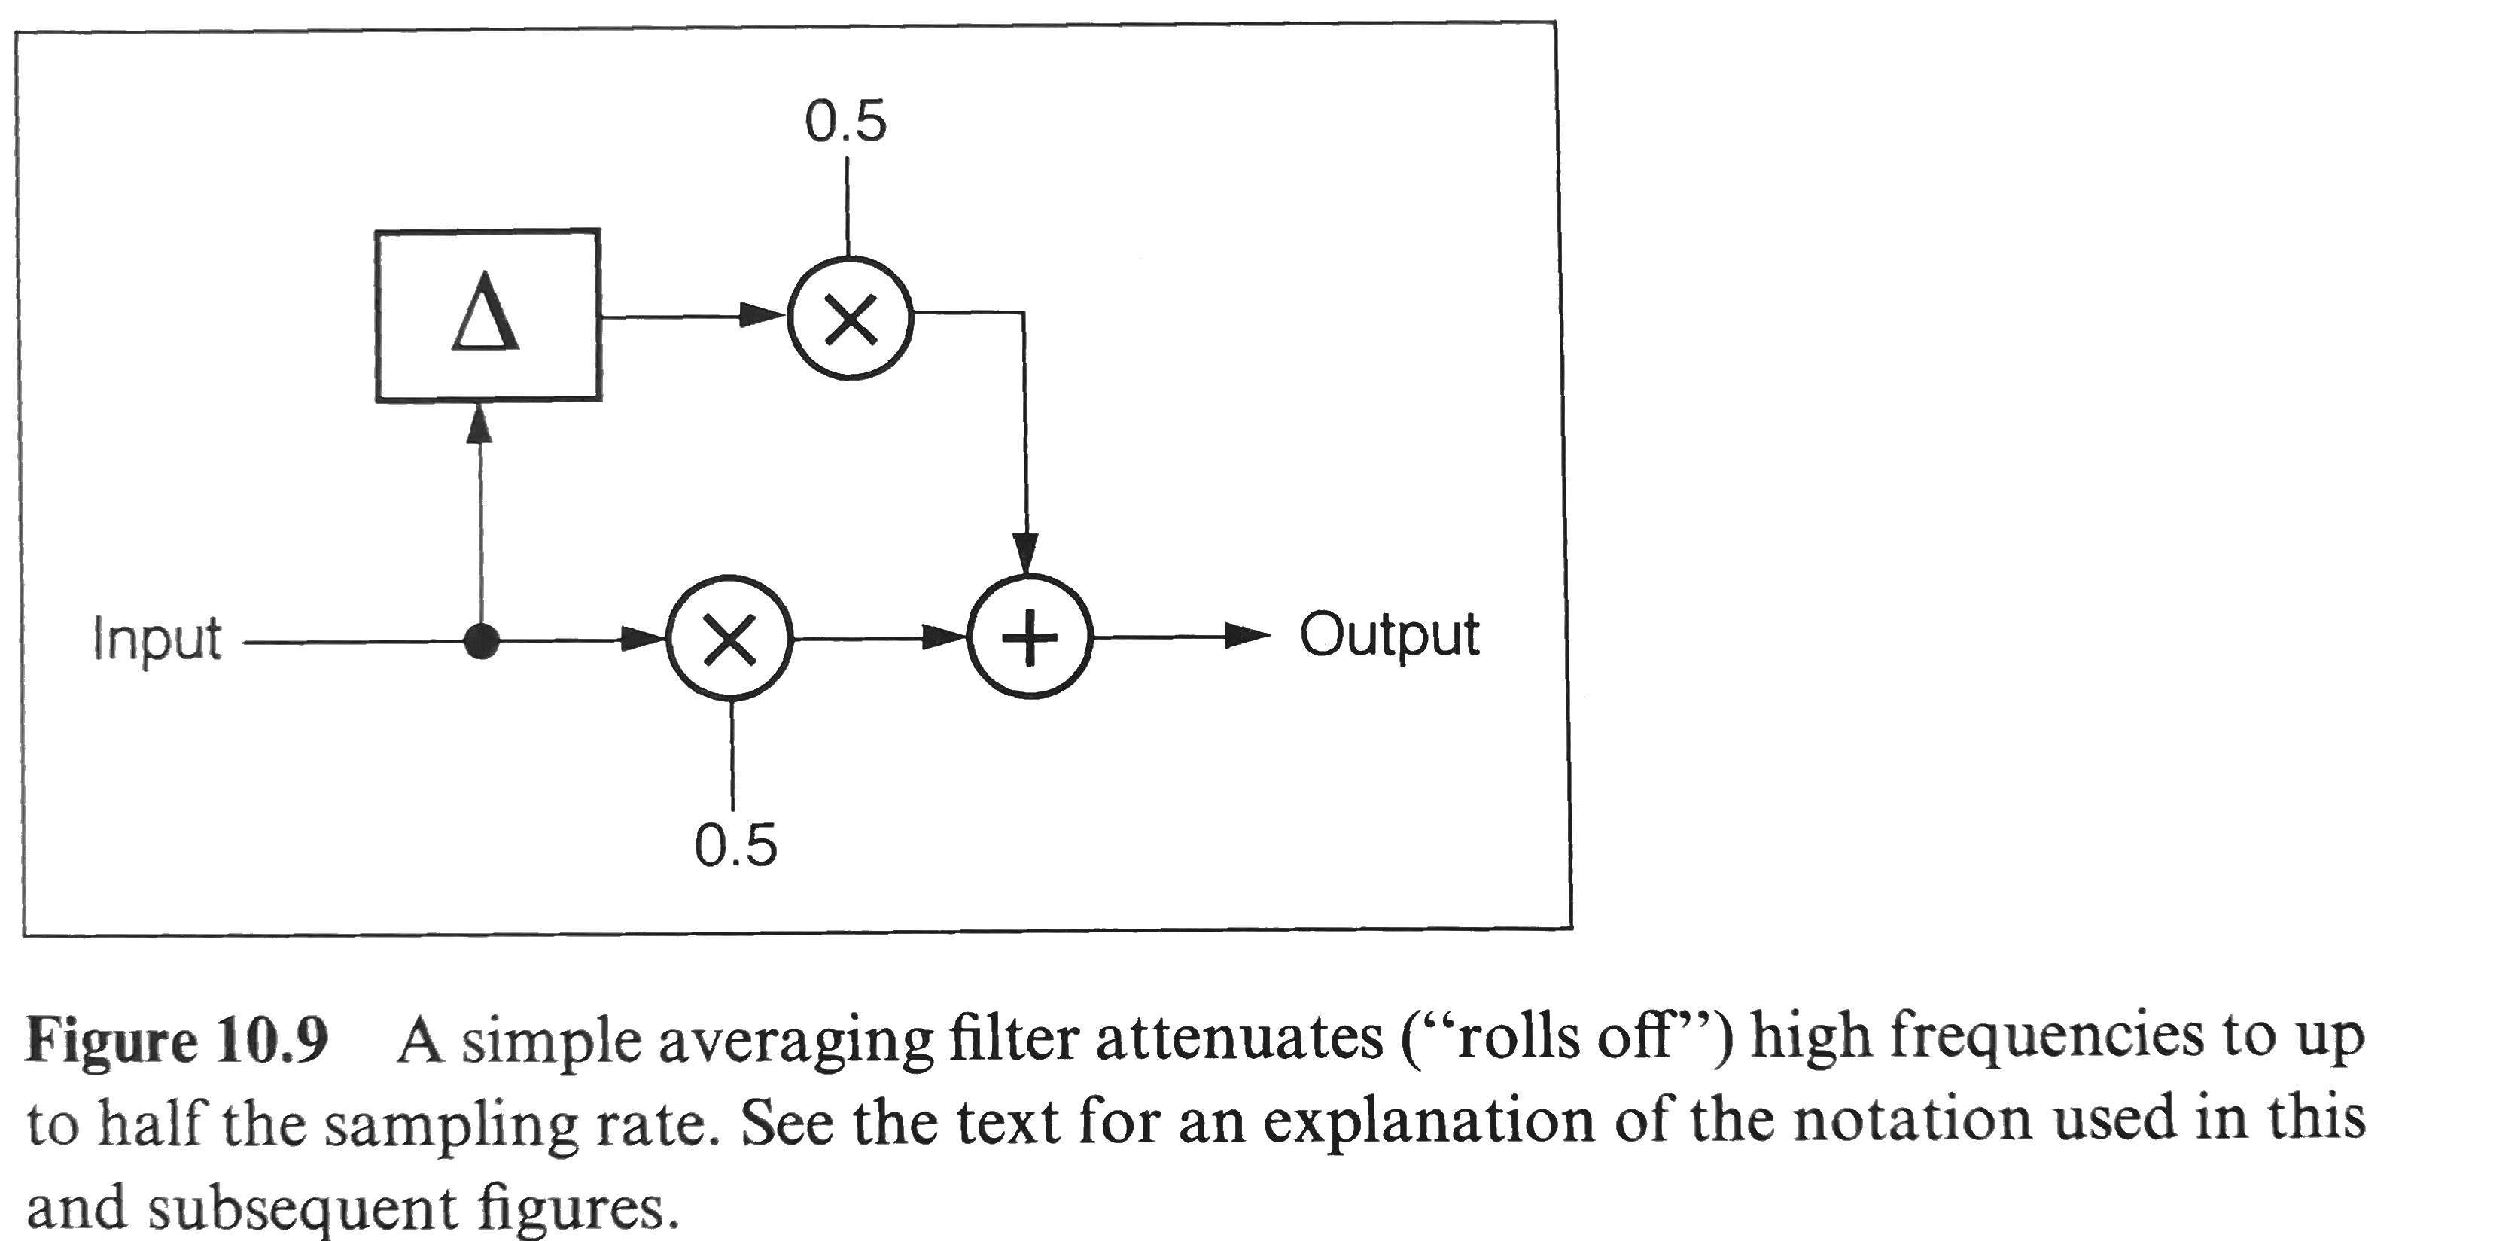
\includegraphics[width=\textwidth]{CAPITOLI/0500/IMG/CT_Lowpass.pdf}
  \caption[]{Lowpass. Computer Music Tutorial.}
  \label{CT-Lowpass}
\end{figure}

L'equazione di un filtro di questo tipo è la sequente:

\begin{equation}
  \label{lowpass}
  y[n] = (0.5 \times x[n]) + (0.5 \times x[n-1])
\end{equation}

dove $y[n]$ è il segnale d'uscita, $(0.5 \times x[n])$ è la metà del campione in
entrata e $(0.5 \times x[n-1])$ è la metà del campione precedente.

La costante di riscalamento ($0.5$) nell'espressione è denominata \emph{coefficiente
del filtro}.

L'equazione trascritta in linguaggio Faust:

\lstinputlisting{CAPITOLI/0500/CODES/lowpass.dsp}

produce il diagramma di flusso:

\begin{figure}[ht]
  \centering
  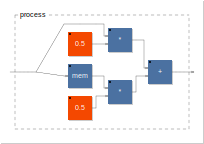
\includegraphics[]{CAPITOLI/0500/CODES/lowpass-svg/process}
  \caption[]{Lowpass. Faust Diagram.}
  \label{fdlowpass}
\end{figure}

Questa la risposta all'impulso:

\lstinputlisting{CAPITOLI/0500/CODES/lowpass.txt}

\clearpage


\clearpage

%!TEX TS-program = xelatex
%!TEX encoding = UTF-8 Unicode
%!TEX root = ../../metp.tex

\section{Processi nel tempo}

Molti processi applicati al suono contemplano ritardi, anche minimi, del segnale
in transito. L'\emph{unità di ritardo}, o la \emph{linea di ritardo}, digitale
prende una serie di campioni e la memorizza per un certo tempo prima di
riprodurla in uscita. Sommare un suono con la sua versione ritardata nel tempo
può causare una serie di effetti musicali che hanno caratterizzato la storia
dell'elaborazione temporale dei suoni.

Nel manuale utente della \emph{Infernal Machine} utilizzata dallo studio di
Friburgo per i live electronics di Luigi Nono, nei paragrafi dedicati alle
operazioni con il delay ci sono esempi di utilizzo per diverse situazioni di
lavoro. Si spiega che si può usare il delay in fase di registrazione per
allineare i microfoni in situazioni di microfonazione multipla, oppure per
creare degli effetti in fase di mix. Si legge sul manuale:

\begin{quote}
  Sommando il suono originale con un lo stesso leggermente in ritardo si
  ottiene un effetto di filtraggio denominato \emph{phasing}. La risposta in
  frequenza in modalità \emph{phasing} si muove continuamente nello spettro
  delle frequenze. Le impostazioni tipiche per questo tipo di effetto vanno dai
  0,04 ai 10 millisecondi.
\end{quote}

Va considerato che il tempo minimo di ritardo dell'unità \emph{Infernal Machine}
era di 0,04 millisecondi (40 microsecondi).

\lstinputlisting{CAPITOLI/0500/CODES/immdt.dsp}



\section{PROCESSI BASATI SU ALL-PASS}

I Phaser sono essenzialmente filtri ladder modulati con LFO costruiti attorno ai
filtri allpass anziché ai filtri passa basso. I flanger possono essere ottenuti
dai phaser con una sostituzione allpass. Per questi motivi entrambi i tipi
appartengono alla discussione sul filtro VA.

\subsection{PHASER}

Il phaser più semplice viene creato mescolando il segnale di input (dry) non
modificato con un segnale filtrato allpass (wet) come nel caso in cui il cutoff
del filtro allpass sia tipicamente modulato da un LFO. Il filtro allpass può
essere piuttosto arbitrario, tranne per il fatto che deve essere un filtro
differenziale.

Nei punti in cui la risposta di fase del filtro allpass i segnali dry si
annulleranno a vicenda, producendo una tacca. la risposta di fase del filtro
allpass è 0◦ i segnali wet e dry si aumenteranno reciprocamente, producendo un
picco (Fig. 6.2).

La struttura del phaser in Fig. 6.1 non contiene feedback, quindi non vi è
alcuna differenza tra implementazioni digitali ingenue e TPT (tranne per il
fatto che i filtri allpass sottostanti dovrebbero essere costruiti meglio in un
modo TPT).

\subsection{Miscelazione a rapporti arbitrari}

Invece di miscelare con il rapporto 50/50, possiamo miscelare con qualsiasi altro rapporto, dove la somma dei guadagni di miscelazione a secco e ad umido dovrebbe ammontare a unità. Ciò influenzerà la profondità delle tacche e l'altezza delle cime. Per il phaser in Fig. 6.1, il rapporto di miscelazione superiore a 50/50 (dove la quantità di segnale bagnato è superiore al 50%) ha poco senso.
Invece di mescolare ydry e ywet con rapporti diversi potremmo semplicemente dissolvere il segnale di uscita tra x (t) e y (t), dove questi sono definiti come in Fig. 6.1. Questo secondo approccio diventerà anche molto più pratico del primo dopo aver introdotto il feedback come in Fig. 6.4.

\subsection{Inversione del segnale bagnato}

Invertendo il segnale bagnato, si scambiano i picchi e le tacche. Si noti che la risposta di fase degli allpass differenziali a ω = 0 può essere 0◦ o 180◦, lo stesso vale per la risposta di fase a ω = + ∞. Per questo motivo potrebbe essere utile la possibilità di scambiare picchi e tacche.

\subsection{Spaziatura tacca}

Nel caso più semplice si usa una serie di allpass identici a 1 polo all'interno di un phaser. Al fine di controllare la spaziatura della tacca in un modo semplice e piacevole, si dovrebbe piuttosto utilizzare una serie di allpass identici a 2 poli. Come accennato in precedenza, modificando la quantità di risonanza dei passaggi a 2 poli si controlla la pendenza di fase dei filtri. Ciò influisce sulla spaziatura delle tacche (Fig. 6.3).

\subsection{Risposta}

Possiamo anche introdurre feedback nel phaser. Analogamente al caso delle modalità filtro ladder, il segnale dry viene raccolto meglio dopo il punto di feedback (Fig. 6.4). Il feedback cambia la forma dei picchi e delle tacche (Fig. 6.5).


\clearpage

%!TEX TS-program = xelatex
%!TEX encoding = UTF-8 Unicode
% !TEX root = ../../metm.tex

\begin{refsection}

\section{Riverberi Digitali}
\thispagestyle{empty}

Nonostante l'acustica architettonica sia stata parte integrante della
progettazione di strutture per millenni, la materia ha ottenuto una base
scientifica solida solo ai primi del novecento per opera di Wallace Sabine.
La definizione del tempo di riverbero da parte di Sabine è il punto di partenza
anche nella letteratura sulla modellazione digitale dell'effetto ad opera di
Manfred Schroeder. Con Sabine il tempo di riverbero può essere descritto,
misurato, previsto. Tutto quello che sappiamo fare oggi continua ad attingere
alle sue ricerce.

\subsection{Sabine}

\subsection{Natural Sounding Artificial Reverberation}

% STAMPA DEI BARPLOT
% bar(faustout);
% xlim ([0 10]);
% set(gca,'fontname','fira', "fontsize", 12);
% grid on;
% xlabel('Time (samples)');
% ylabel('Amplitude');
% set(gca,'XTick',0:1:10);
% print -dpng dfl.png

Come per Sabine, Schroeder rende possibile un avanzamento scientifico legato
al riverbero approcciando alla soluzione di alcuni problemi di stabilità e
linearità inn requenza dei riverberi disponibili all'epoca. È consapevole delle
necessità, che mette in chiaro fin dal principio: diffusione di un riverbero
necessita di un numero minimo di $1000$ echi per secondo per non esprimere fastidiose
fluttuazioni. Inoltre questa diffusione deve avvenire senza distruggere il
contributo timbrico della sorgente, cosa che accadeva spesso con i riverberi
elettronici dell'epoca.

\begin{figure}[hb]
  \centering
  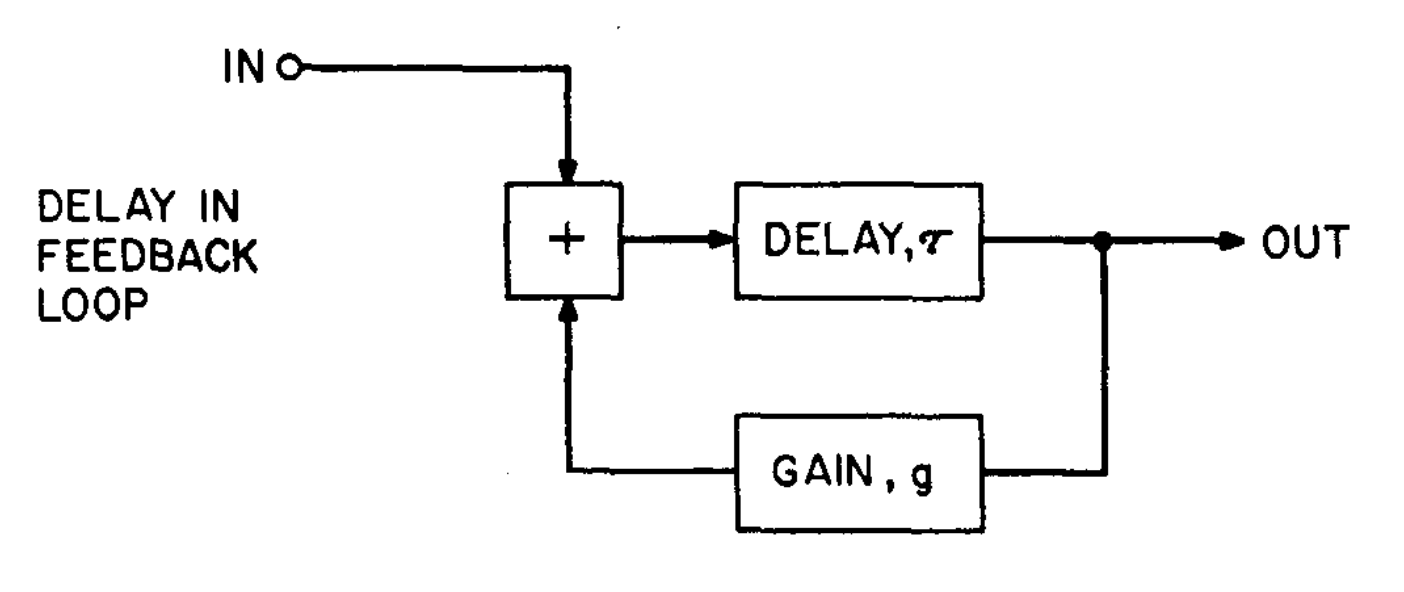
\includegraphics[width=\textwidth]{CAPITOLI/0500/IMG/dfl.png}
  \caption[]{Delay in Feedback Loop. Schroeder, 1962.}
  \label{schroeder:dfl}
\end{figure}

Il percorso di costruzione di questo sistema di riverberazione parte dalla
più semplice delle strutture ricorsive di filtraggio: il
\emph{filtro passa basso IIR} al quale non si da un solo campione di ritardo,
ma un ritardo variabile, che ne cambia il comportamento temporale e quindi
spettrale.

\begin{figure}[t!]
  \centering
  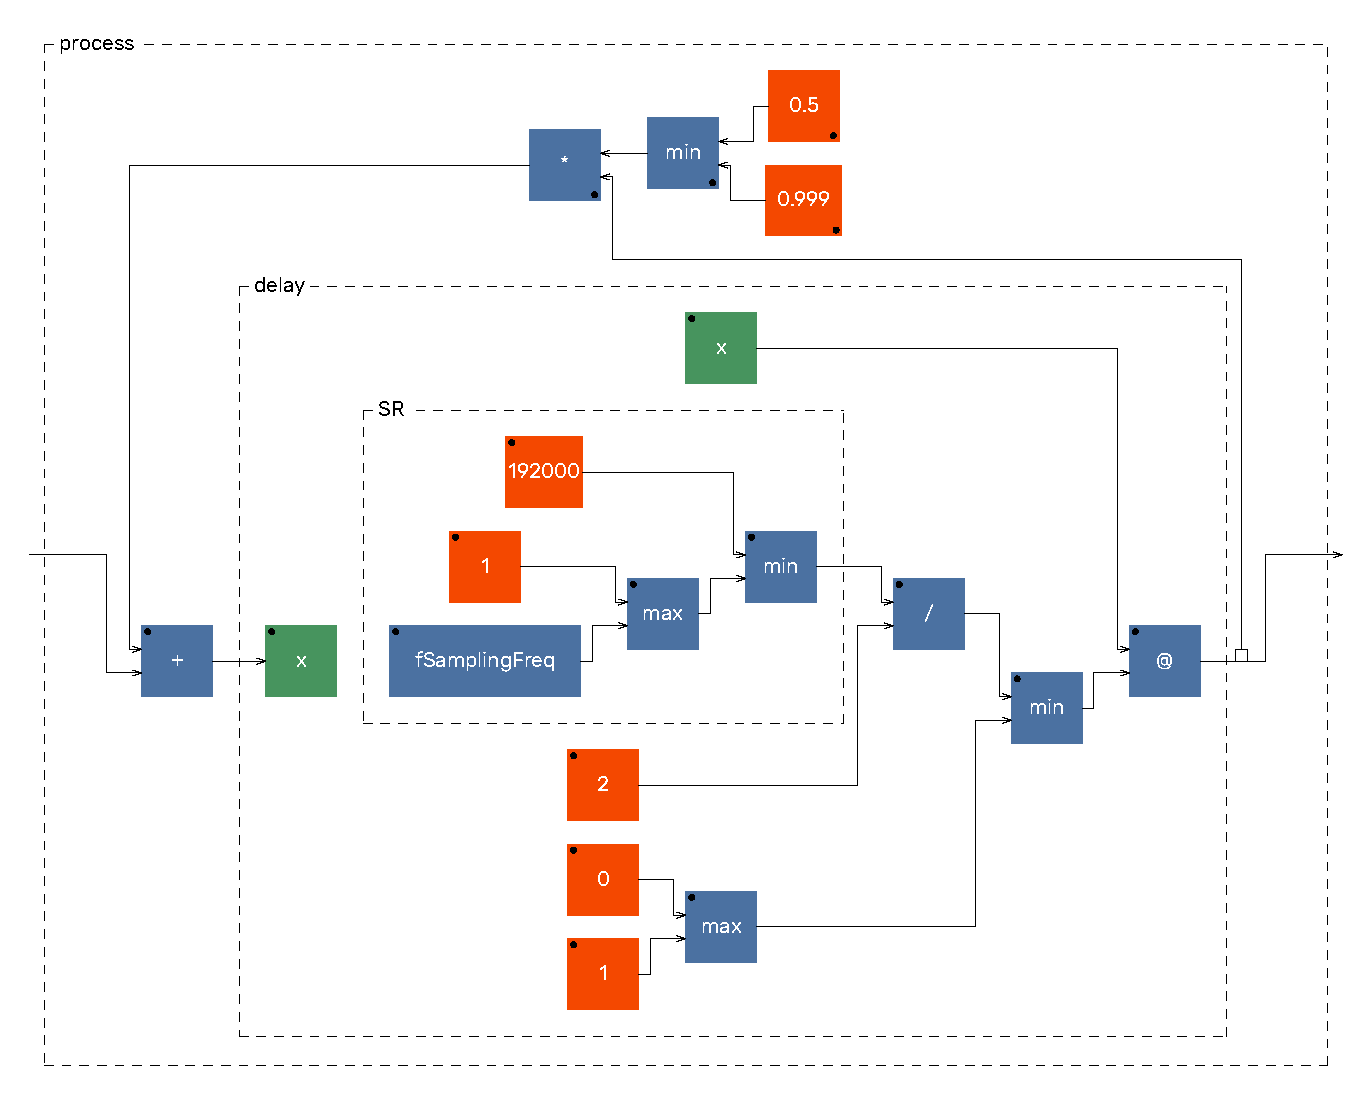
\includegraphics[width=\textwidth]{CAPITOLI/0500/CODES/REV/dfl-svg/process.pdf}
  \caption[]{Delay in Feedback Loop. Implementazione Faust.}
  \label{faust:dfl}
\end{figure}

Il primo oggetto che Schroeder descrive è quindi una linea di ritardo
alimentata da un circuito di retroazione controllato dal coefficiente $g < 1$.

Il filtro prevede un valore di ritardo $t$ applicato a tutti i campioni in
entrata, situazione che può avere diversi significati, come cercherò di spiegare
in seguito.

Il codice Faust per la realizzazione di tale oggetto è il seguente.

\lstinputlisting{CAPITOLI/0500/CODES/REV/dfl.dsp}

Il codice di descrizione della funzione è presente tutto in riga tre, la quale
può essere smontata in più parti per comprenderne la sintassi.

Il blocco di ritardo \texttt{delay} deve essere inizializzato con l'allocazione
di memoria massima in campioni. L'impostazione inserita \texttt{SR/2} permette
di avere almeno mezzo secondo a qualsiasi requenza di campionamento. Il tempo
$t$ di ritardo effettivo, in quanto unità al campione, deve essere necessariamente
un intero, motivo per cui la variabile in entrata $t$ viene passata per una
funzione \texttt{int} che ne scarta eventuali valori decimali.

L'uscita del blocco di ritardo viene prelevata prima dell'uscita dal filtro e
reindirizzata alla sua entrata, adeguatamente scalata dal coeffficiente $g < 1$,
in somma con l'entrata del filtro.

\begin{figure}[ht]
  \centering
  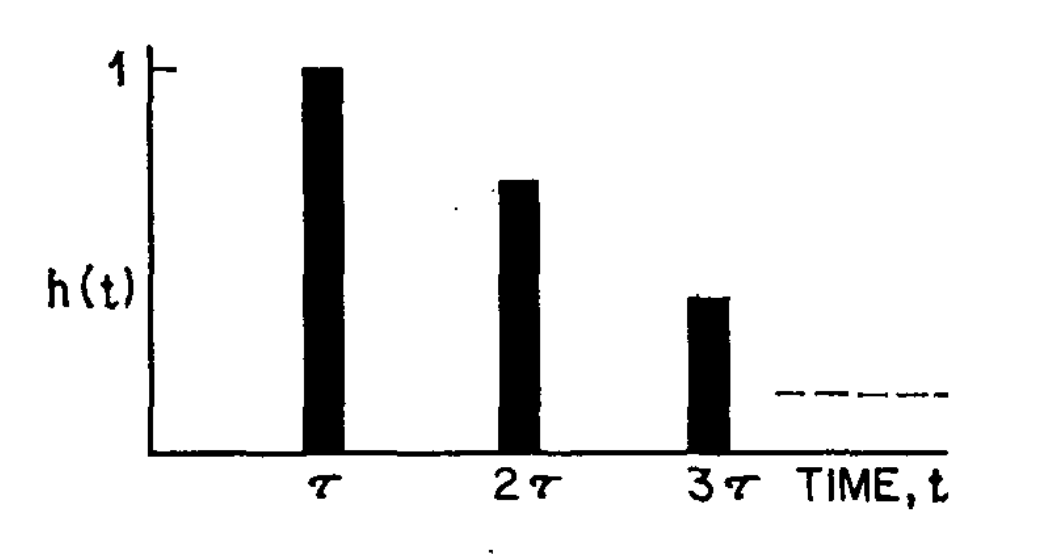
\includegraphics[width=\textwidth]{CAPITOLI/0500/IMG/dfl-ir.png}
  \caption[]{Schroeder dfl impulse response.}
  \label{schroeder:dflir}
\end{figure}

Schoreder fornisce una chiara descrizione del funzionamento temporale del filtro
ed attraverso un diagramma ne mostra la risposta all'impulso. La figura
\ref{schroeder:dflir} mostra il comportamento del filtro ad un tempo $t$
consistente in ripetizioni successive per multipli interi $2t$, $3t$ \ldots fino
al completo esaurimento dell'ampiezza per opera del coefficiente scalare $g$.

\begin{figure}[ht]
  \centering
  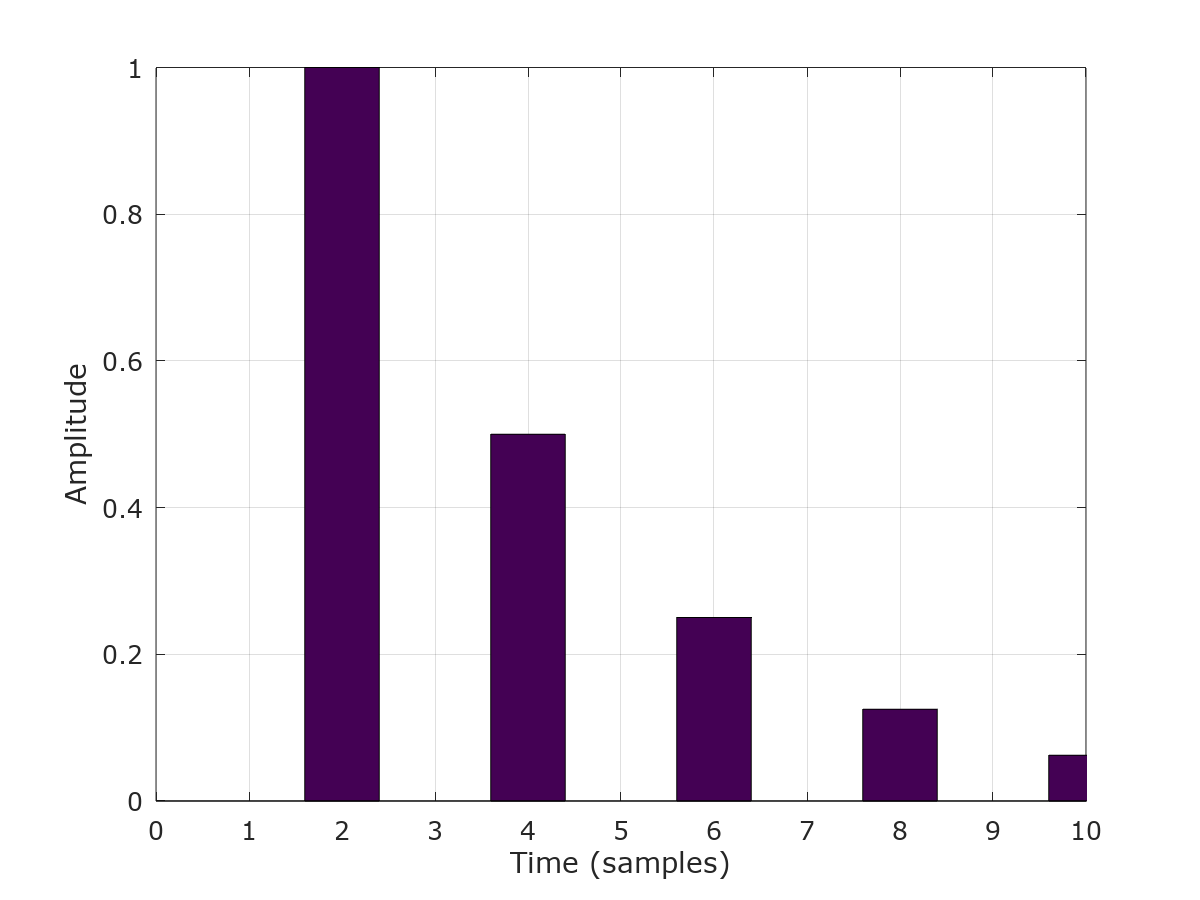
\includegraphics[width=\textwidth]{CAPITOLI/0500/CODES/REV/dfl.png}
  \caption[]{Faust dfl impulse response.}
  \label{faust:dflir}
\end{figure}

La risposta all'impulso illustrata in figura \ref{schroeder:dflir} indica un
decadimento esponenziale per ogni riflessione eco.

Possiamo descrivere allo stesso modo il nostro modello: il tempo di ritardo $t$
regola le nuove occorrenze dell'impulso generate dal circuito di retroazione
scalate dal coefficiente $g$. Pur avendo creato un modello di filtro
apparentemente identico, producente un diagramma a blocchi \ref{faust:dfl}
piuttosto fedele al modello di Schroeder, la risposta all'impulso del nostro
filtro si comporta in modo diverso, motivo per cui merita uno sguardo di analisi
e un'attenta riflessione.

La risposta all'impulso di figura \ref{faust:dflir} è stata generata impostando
le variabili $t=1$ (un campione di ritardo) e $g=0.5$ (ampiezza dimezzata ad
ogni giro di feedback). Ci si aspetta quindi un comportamento molto simile a
quello descritto da Schroeder, per una successione di multipli di $1$ dovremmo
avere il primo impulso nella posizione $n[1]$ con ampiezza $a=1$ (non scalata,
non l'impulso non è ancor transitato nel ciclo di ffeedback). Il secondo impulso
dovrebbe essere posizionato subito dopo il primo, nella posizione $n[2]$ con
ampiezza $a=0.5$, e cosi proseguendo. Tuttavia, osservando l'indicizzazione dei
campioni sull'asse delle ascisse della figura \ref{faust:dflir} si può constatare
che in realtà il nostro filtro sta impiegando due campioni per ogni ciclo
impulsivo in luogo di uno, posizionando gli impulsi per $2t$.

La motivazione di questa differenza è nascosta dietro al significato del diagramma
a blocchi di entrambe le rappresentazioni. Nella prima, quella originaria di Schroeder,
il punto di prelievo del segnale per il ciclo di feedback è a tempo zero, ovvero
linea che porta il segnale dall'uscita del blocco di ritardo all'entrata della
somma è istantanea. Nella descrizione algoritmica di faust mediante diagramma
a blocchi invece l'operatore $~$ produce contestualmente al prelievo del segnale,
un inevitabile campione di ritardo. La linea di ricircolo quindi, nel momento
in cui alimenta il blocco di ritardo, porta già un campione di ritardo su quello
corrente.

La correzione di questo filtro per ottenere il comportamento prospettato da Schroeder
consiste nel sottrarre il campione di ritardo, prodotto dalla ricorsione, alla
variabile $t$ con $t-1$. Questo tipo di intervento per $t=$ produrrà $t=1-1=0$
ovvero zero campioni di ritardo all'uscita, un campione, come richiesto,
scalato in $g$ all'entrata della somma di ricircolo. Questo tipo di operazione
crea però un offset temporale in quanto la sequenza di campioni ritardati, ora
corretta, si trova in uscita un campione prima (ritardo zero) di quello richiesto.
Anche questa problematica è risolvibile inserendo un ulteriore campione di ritardo
\texttt{mem} all'uscita dell'algoritmo, in modo da bilanciare l'intera sequenza
temporale.

\lstinputlisting{CAPITOLI/0500/CODES/REV/dflc.dsp}

La risposta all'impulso del filto corretto è ora coerente con le aspettative.

\begin{figure}[ht]
  \centering
  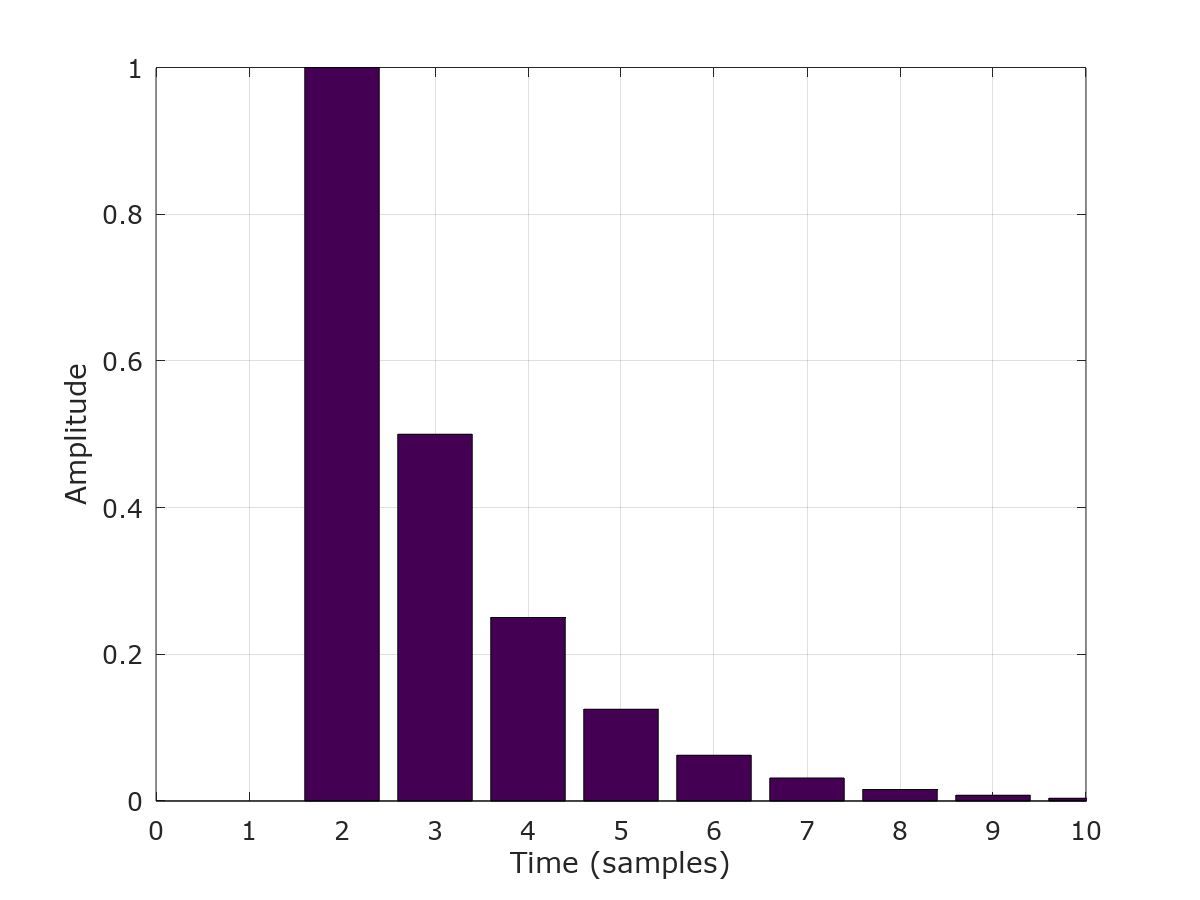
\includegraphics[width=\textwidth]{CAPITOLI/0500/CODES/REV/dflc.png}
  \caption[]{Faust dfl impulse response.}
  \label{faust:dflir}
\end{figure}

Il filtro appena costruito può operare tempi di ritardo tra $1$ e \emph{Nyquist}.
Questo comportamento può portare a diversi risultati sonori, dal più diretto
ritardo di una quantità di campioni indicata con $g=0$, oppure ad un filtraggio di componenti
spettrali in funzione di $t$ e $g$.

\begin{figure}[h]
  \centering
  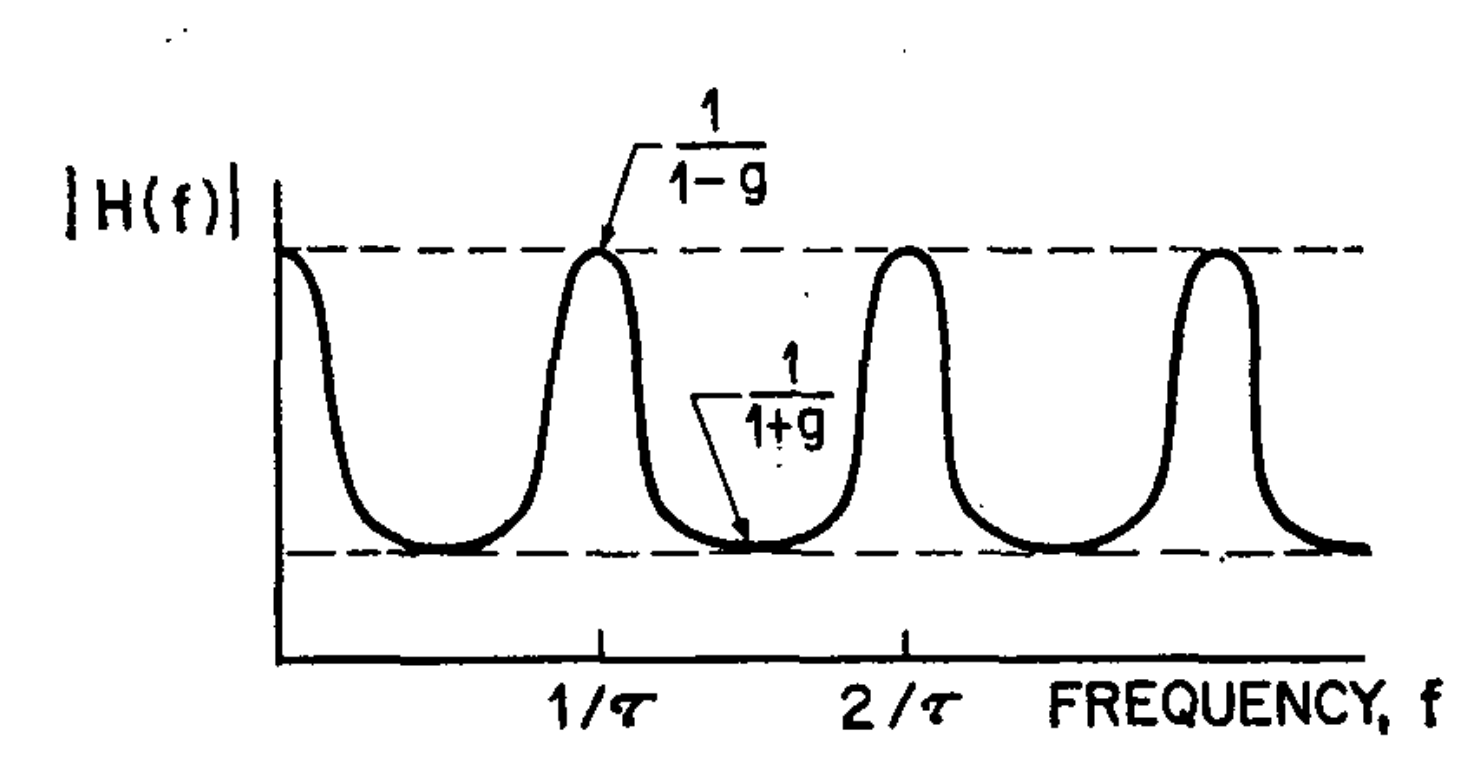
\includegraphics[width=\textwidth]{CAPITOLI/0500/IMG/dfl-fr.png}
  \caption[]{Schroeder dfl risposta in requenza, \emph{”somigliante ad un pettine”}.}
  \label{schroeder:dflffr}
\end{figure}

\begin{quote}
  The amplitude-frequency responce has the appearance of a comb with periodic
  maxima and minima\ldots It is these peaks and valleyys which impart the undesidered
  “colored” qualityy to sound reverberated by devices like that.
\end{quote}

Il rapporto tra la risposta massima e quella minima è espresso dalla formula:

\begin{equation}
  \label{comb-filter}
  H_{max}/H_{min} = (1+g)/(1-g)
\end{equation}

il che porta a considerare che per un coefficiente $g=0.708$ corrispondente ad
un abbattimento di $-3dB$ il rapporto di di $5.849:1$ (espresso da $1.708/0.292$)

\begin{equation}
  \label{hmax}
  \Delta_{amp} = 20\times Log_10(5.849) = 15.34 dB
\end{equation}

ovvero $15.34dB$ di escursione.

\begin{quote}
  In a search for better artificial reverberators\ldots (we) noted that certain
  mixture of the output of the multiply delayed sound and the undelayed sound
  would result in an equal response of the reverberator for all frequencies.
\end{quote}

Questo passo è cruciale per comprendere il processo evolutivo dei meccanismi
riverberanti di Schroeder. Il filtro IIR passa da un campione di ritardo (passa
basso) ad un delay variabile (comb-filter) e sta per diventare un filtro
lineare in frequenza (all-pass) attraverso una oculata gestione dei rapporto tra
suono diretto e suono ritardato. La proporzione per contenere l'energia unitaria
su tutto lo spettro di frequenze è $-g$ per il segnale diretto e $1-g^2$
per il segnale ritardato.

\begin{figure}[ht]
  \centering
  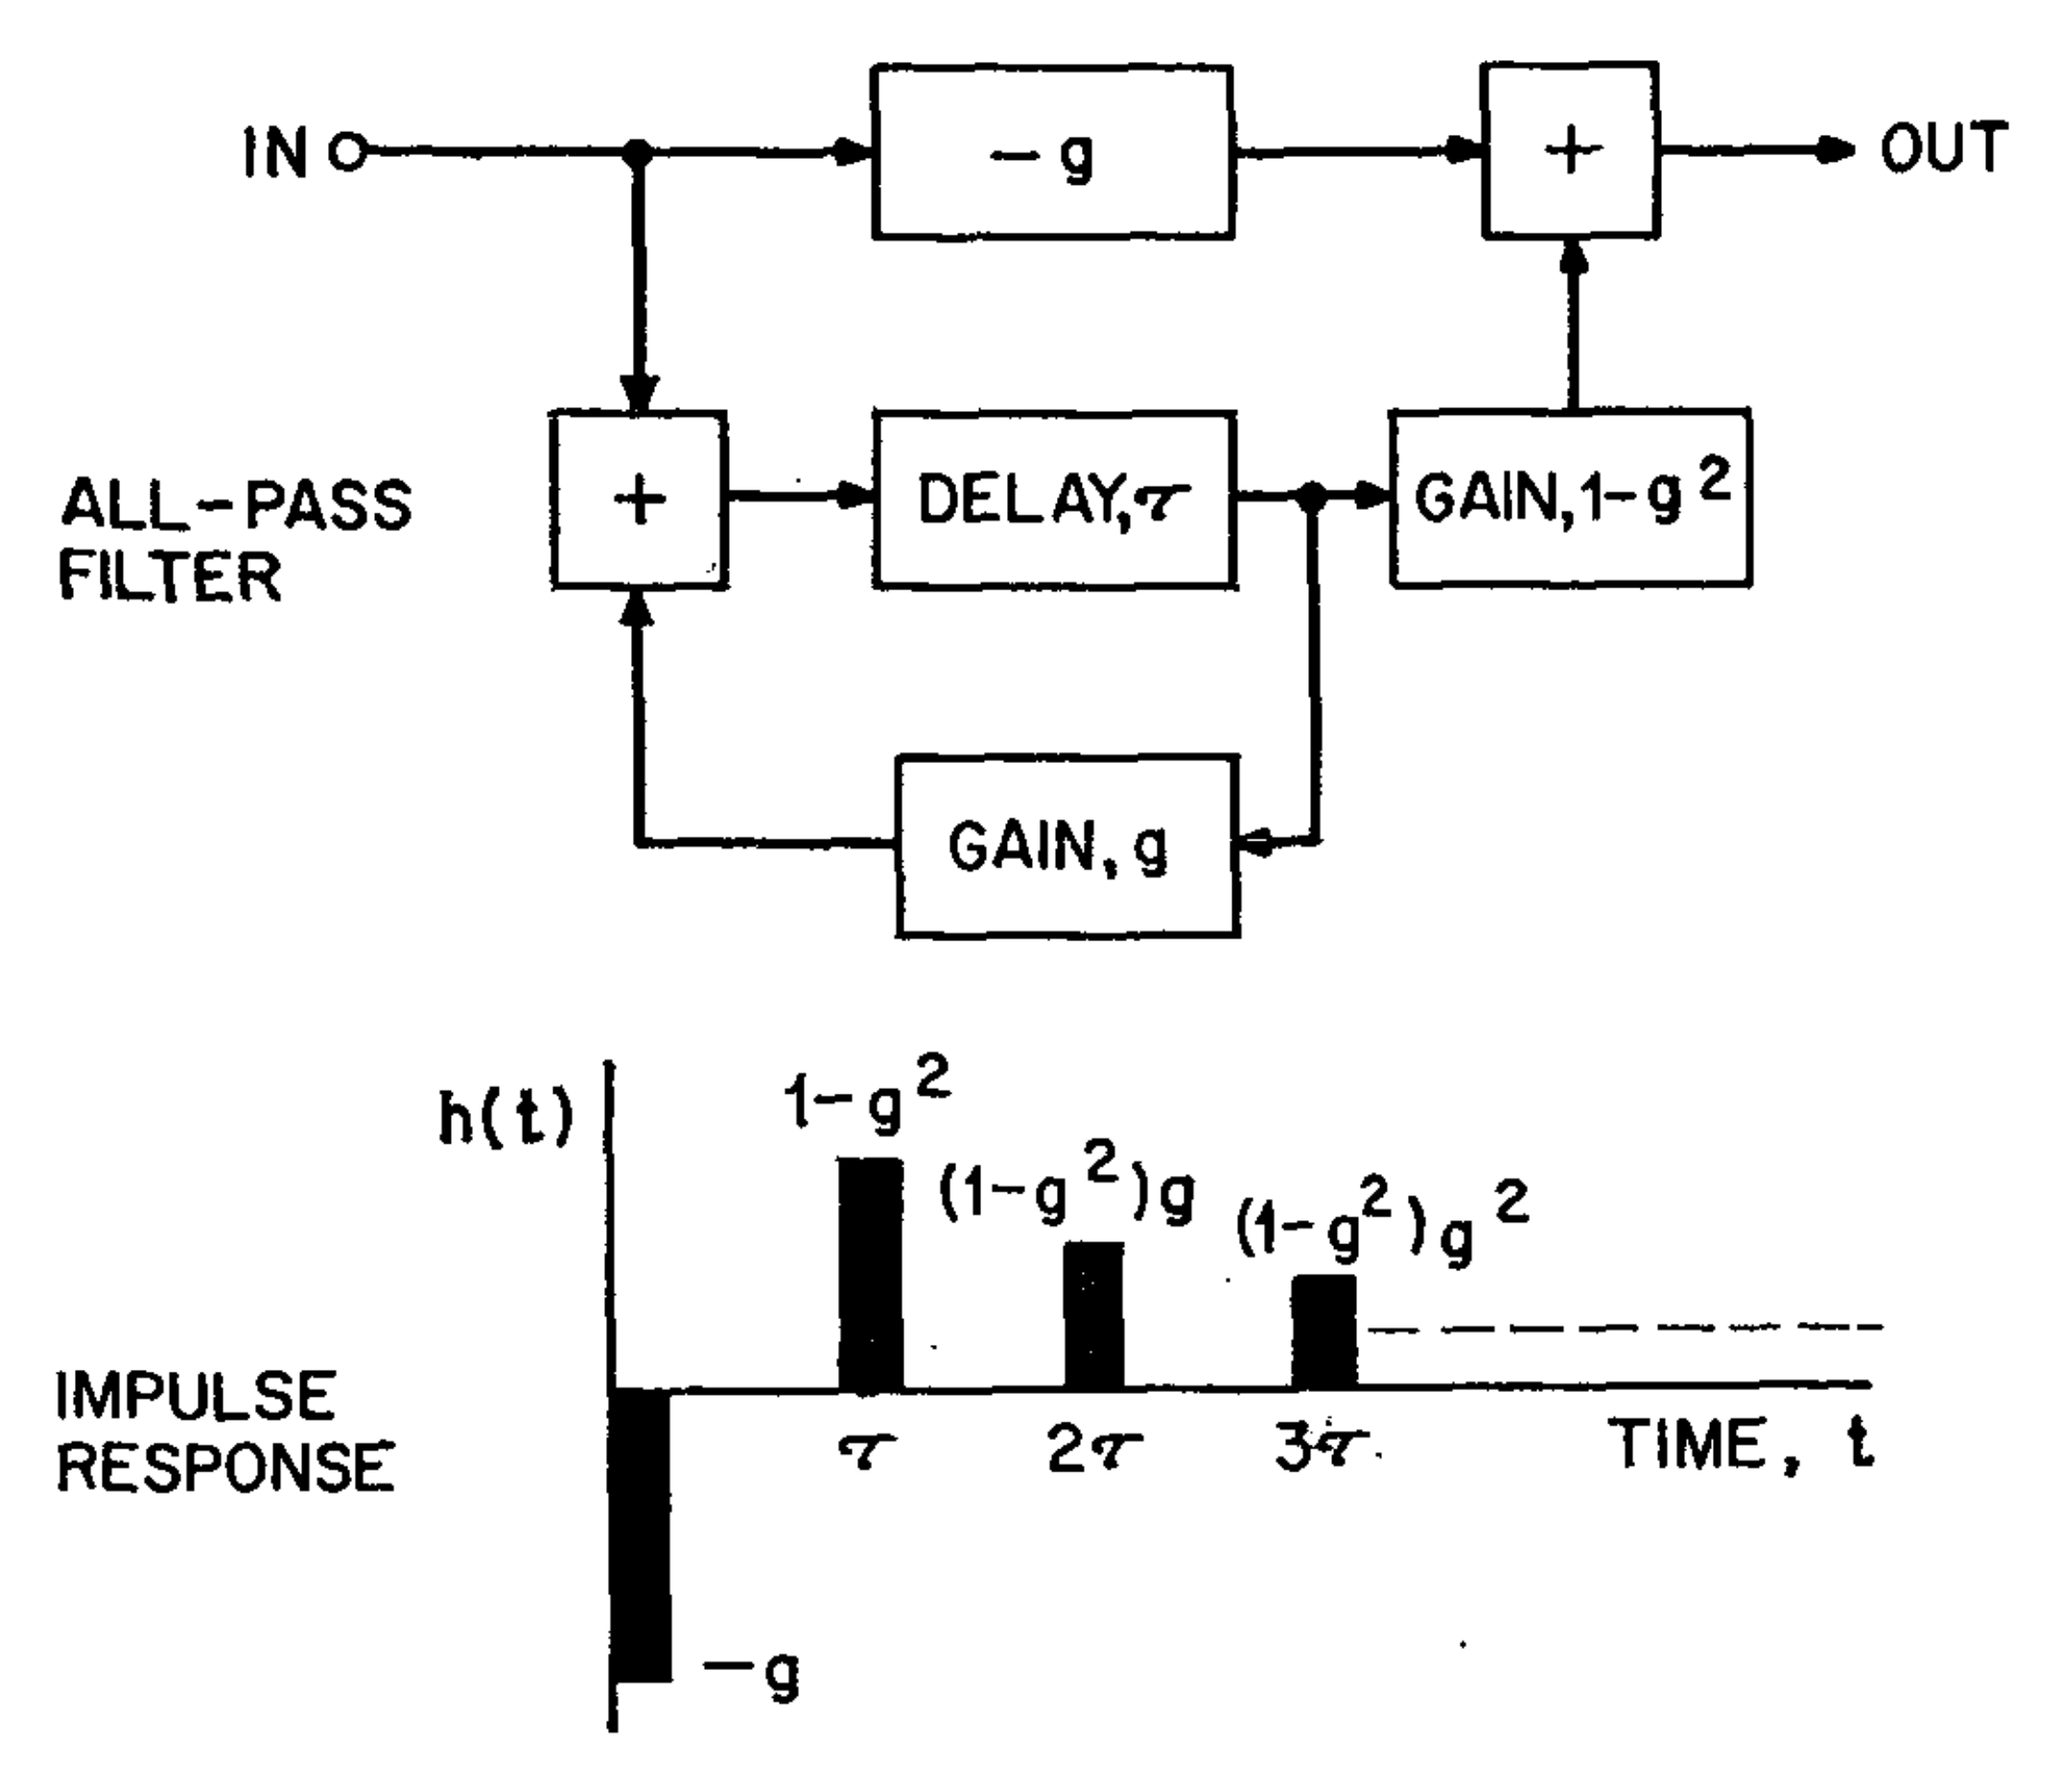
\includegraphics[width=\textwidth]{CAPITOLI/0500/IMG/allpass.png}
  \caption[]{All-pass, diagramma a blocchi e risposta all'impulso.}
  \label{schroeder:allpass}
\end{figure}

\begin{quote}
  \ldots the addition of a suitably proportioned uunudelayyed path has converted
  the comb-filter (fig. \ref{schroeder:dfl}) into an all-pass (fig.
  \ref{schroeder:allpass}). This is not a mere academic result.
\end{quote}

Il filtro all-pass ora permette di passare tutte le frequenze con eguale ampiezza
e senza “colorare” il segnale. Si possono connettere tra loro diverse unità di
questo tipo per raggiungere la densità di eco necessaria. Inoltre il filtro
all-pass condivide con i filtri comb le proprietà del feedback e del decadimento
esponenziale dell'energia, lo stesso comportamento che si presenta nelle buone
situazioni acustiche.

\lstinputlisting{CAPITOLI/0500/CODES/REV/apf.dsp}

\printbibliography
\end{refsection}



%!TEX TS-program = xelatex
%!TEX encoding = UTF-8 Unicode
% !TEX root = ../metm.tex

\chapter{ANALISI}
\startcontents[chapters]
\printcontents[chapters]{}{1}{}


%!TEX TS-program = xelatex
%!TEX encoding = UTF-8 Unicode
% !TEX root = ../metm.tex

\chapter{SINTESI}
\startcontents[chapters]
\printcontents[chapters]{}{1}{}

%!TEX TS-program = xelatex
%!TEX encoding = UTF-8 Unicode
% !TEX root = ../../metm.tex

\section{OSCILLATORE VIRTUALE}

L’oscillatore virtuale è un algoritmo che legge e invia in uscita,
ciclicamente, i campioni (dati quantizzati) di una forma d’onda.
Tutti i campioni che rappresentano un periodo della forma d’onda,
sono scritti precedentemente in un area di memoria chiamata tabella o table look-up.

Considerando il teorema del campionamento1 si possono seguire i seguenti passi per implementare un oscillatore virtuale:
1.- Si calcolano i valori dei campioni corrispondenti ad un ciclo della forma d’onda.
2.- Vengono memorizzati i valori in una tabella. Essa conterrà un ciclo di un' onda memorizzata in n locazioni di memoria. Ciascuna locazione è contrassegnata da un indice, indicato dai numeri interi.
3.- Si rileggono in sequenza i campioni, ciclicamente e ad un valore prefissato di frequenza di campionamento.


Obiettivi:

Implementing a sine oscillator from scratch in Faust
Understand the relation between the sine function and the generated sound
Use multiple sine oscillator to implement an additive synthesizer
Use SmartKeyboard to produce polyphonic mobile apps to control this synth

Referenze:
Manuale \emph{Faust}
computer music tutorial

\subsection{Funzione \emph{seno}}

\begin{figure}[ht]
  \centering
  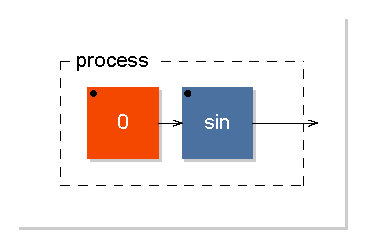
\includegraphics[]{CAPITOLI/0700/CODES/0701-seno-svg/process}
  \caption[]{Sine function. Faust Diagram.}
  \label{fdsine}
\end{figure}

\lstinputlisting{CAPITOLI/0700/CODES/0701-seno.dsp}

Questi sono i primi 5 campioni prodotti dalla formula $sin(0)$:

\lstinputlisting{CAPITOLI/0700/CODES/0701-seno.txt}

\lstinputlisting{CAPITOLI/0700/CODES/0702-senopi2.dsp}

Questi sono i primi 5 campioni prodotti dalla formula $sin(\pi/2)$:

\lstinputlisting{CAPITOLI/0700/CODES/0702-senopi2.txt}

questi i campioni

\lstinputlisting{CAPITOLI/0700/CODES/0703-senovariopi.txt}



%!TEX TS-program = xelatex
%!TEX encoding = UTF-8 Unicode
% !TEX root = ../metm.tex

\chapter{IL REPERTORIO}
\startcontents[chapters]
\printcontents[chapters]{}{1}{}

ciao\footcite[\emph{idem}]{prieberg:mexm}

Agamben \index[names]{Agamben, Giorgio}

\section{Luigi Nono}

NONO, Luigi (Venezia, 29.1.1924 – Venezia, 8.5.1990)

Nato il 29 gennaio 1924 a Venezia, primogenito di Mario Nono e Maria Manetti. Nono ebbe già nell’ambito familiare i primi stimoli per la sua formazione artistica e culturale: il nonno paterno, Luigi Nono, era un noto pittore della scuola veneziana di fine Ottocento; il prozio Urbano (fratello del pittore) uno scultore; la nonna materna, discendente dell’antica famiglia veneziana Priuli Bon, si dilettava col pianoforte e col canto spaziando dalla musica del passato alla produzione liederistica più recente (Nono ricorderà con stupore di aver rinvenuto tra i suoi spartiti una delle prime edizioni degli Italienische Lieder di Hugo Wolf accanto al Montezuma di Sacchini; Nono 1987, p. 480). La madre e il padre, di professione ingegnere, erano pianisti dilettanti che amavano cimentarsi con brani di repertorio (tra questi, il Boris Godunov di Modest Musorsgkij, spesso ricordato tra i primi ascolti nella sua fanciullezza; ibid.). Frequentatori assidui del Teatro La Fenice e di varie rassegne concertistiche, Mario e Maria Nono erano inseriti nei circoli culturali e musicali della migliore società veneziana. Grazie alla fornita discoteca del padre, Nono poté conoscere presto la musica di Beethoven, Wagner, Mahler nelle prime incisioni di direttori quali Toscanini o Mengelberg. Di non minore importanza furono le prime erratiche letture condotte sui libri della imponente biblioteca paterna (oggi in parte conservati nel lascito del compositore), dalle prime traduzioni italiane di poeti e scrittori russi, ai romanzieri americani pubblicati all’epoca da Einaudi, a Pavese, Gogol’, Rilke e vari altri autori che riaffioreranno nel corso degli anni tra le selezioni testuali delle proprie opere. In questa sfaccettata e privilegiata realtà domestica è possibile ravvisare l’origine di quella che diventerà una cifra caratteristica dell’universo artistico noniano, proiettato verso un’idea (e una pratica) della musica intesa come un’arte senza frontiere che può trovare ispirazione e fondamento in varie manifestazioni artistiche e scientifiche (pittura, architettura, letteratura, poesia, filosofia ecc.) delle diverse epoche storiche.

Intorno ai dodici anni Nono intraprese lo studio del pianoforte con una docente privata amica della madre (la signora Alessandri) e, fin da ragazzo, cominciò ad assistere agli spettacoli della Fenice e del Festival internazionale di musica contemporanea della Biennale di Venezia. Svolse i suoi studi presso il Ginnasio-Liceo classico «Marco Polo» di Venezia dove conseguì la maturità nel 1942. Nello stesso anno, per assecondare i desideri del padre, preoccupato delle incertezze della professione musicale, Nono si iscrisse alla Facoltà di Giurisprudenza dell’Università di Padova. Sempre nel 1942 egli conobbe il giovane pittore Emilio Vedova e intrecciò con lui un’amicizia che, rafforzatasi nel tempo anche grazie a varie collaborazioni artistiche, durò a fasi alterne fino alla morte del compositore.

La formazione scolastica e musicale di Nono si svolse negli anni cruciali del secondo conflitto mondiale e dell’immediato dopoguerra, in un clima familiare e intellettuale di stampo tradizionale e borghese ma perlopiù ostile al fascismo. Per motivi di salute egli fu dispensato dal servizio militare e non partecipò attivamente né alla guerra né alle successive fasi della Resistenza. Nono privilegiò nondimeno in quegli anni il contatto con giovani socialisti veneziani e personalità dell’opposizione locale, coltivando ideali politici e culturali non allineati con il regime.

Nel 1941, all’età di 17 anni, il padre gli procurò un incontro con una delle maggiori personalità musicali del tempo, Gian Francesco Malipiero, compositore che gli «aprì tutti gli orizzonti della musica» (Nono 1961, p. 3). Per qualche anno Nono seguì come studente esterno i suoi corsi di Composizione presso il Conservatorio di musica Benedetto Marcello di Venezia; dal 1943, dopo il ritiro di Malipiero dall’insegnamento di composizione, continuò a frequentare sempre da esterno la classe di contrappunto e fuga di Raffaele Cumar (ex allievo di Malipiero e Dallapiccola), approfondendo contemporaneamente in privato lo studio del pianoforte con Gino Gorini. In un periodo segnato culturalmente da una progressiva chiusura verso le esperienze d’avanguardia sviluppatesi in Europa dagli inizi del XX secolo, gli orizzonti aperti da Malipiero riguardavano lo studio di Monteverdi e della grande tradizione rinascimentale italiana (polifonica e madrigalistica), dei trattati teorici di Zarlino, Gaffurio e Vicentino, nonché la scoperta della musica di Arnold Schönberg, Anton Webern e Béla Bartók. Per la sua indole curiosa e irrequieta, Nono non riuscì mai ad adattarsi a piani di studio imposti e, ben presto, cominciò a nutrire una vera avversione per vincoli formativi legati a programmi ministeriali reputati noiosi e spesso inutili. Dopo il conseguimento del compimento inferiore e medio di composizione – sostenuti rispettivamente nel 1947 e 1949 presso il Conservatorio «Benedetto Marcello» – egli non reputò necessario coronare la sua formazione musicale con il diploma.

Nel 1946, grazie a Malipiero, Nono entrò in contatto con il giovane compositore e direttore d’orchestra veneziano Bruno Maderna, di soli quattro anni più anziano, già noto per il suo passato di fanciullo prodigio. All’incirca nello stesso periodo conobbe inoltre Luigi Dallapiccola, tra i musicisti più stimati e punto di riferimento per molti giovani della sua generazione. Delle prove compositive portate a termine prima del fondamentale incontro con Maderna resta solo la labile traccia di un ricordo (Nono 1979-80): nel 1945, durante la frequentazione di Malipiero – e influenzato anche dai suoi lunghi discorsi sulla musica del XV e XVI secolo –, Nono compose La discesa di Cristo agli inferi, brano (in seguito smarrito) forgiato sul modello delle sacre rappresentazioni e ispirato a un linguaggio di stampo monteverdiano (ivi, p. 242). Lo stimolo per il primo decisivo mutamento di rotta, dopo circa otto anni di studi musicali reputati parziali e insufficienti, sembrerebbe esser stato fornito proprio da un parere critico di Dallapiccola sulla partitura de La discesa di Cristo agli inferi, speditagli dal giovane compositore su suggerimento di Malipiero: «capisco che lei ha qui dentro nel cuore molto da esprimere, soltanto deve studiare ancora molto per poterlo esprimere» (ibid.). Queste parole costituirono per Nono una spinta a ricominciare gli studi musicali pressoché da zero in un nuovo periodo di apprendistato con Maderna. Conclusi gli studi universitari – coronati nel 1947 da una laurea in giurisprudenza con una tesi sul concetto giuridico dell’exceptio veritatis – egli poté dedicarsi solo alla musica e indirizzare il suo apprendistato verso un sentiero di conoscenza autonomo e responsabile, condotto al di fuori di ogni istituzione scolastica o accademica. (Di questo periodo 1946-47 non sono note composizioni al di fuori di un progetto vocale su liriche tratte da L’allegria di Giuseppe Ungaretti, poeta da tempo amato e ammirato.)

L’incontro con Maderna segnò in modo indelebile lo sviluppo musicale e umano di Nono, che riconobbe fino alla fine all’amico il ruolo di primo vero e grande maestro di vita.

Durante lunghe giornate trascorse tra l’abitazione di Maderna e la Biblioteca Marciana di Venezia, Nono approfondì – insieme ad altri giovani raccolti intorno al giovane maestro (Romolo Grano, Gastone Fabris e Renzo Dall’Oglio tra questi) – lo studio della musica del XV-XVI secolo, dall’ars antiqua all’ars nova francese, dai fiamminghi alla polifonia rinascimentale italiana, in un continuo confronto tra teoria e pratica. Tra gli autori più amati e analizzati: Guillaume de Machaut, John Dunstable, Johannes Ockeghem, Josquin Desprès, Adrian Willaert, Andrea e Giovanni Gabrieli, spesso trascritti a partire dall’Odhecaton di Ottaviano Petrucci. L’analisi di questo periodo storico divenne – tra la fine degli anni Quaranta e l’inizio del decennio successivo – lo stimolo per un’indagine comparata dei vari processi compositivi nella storia: data la comprensione di una tecnica musicale, il fine era scoprirne la funzione in relazione al momento storico, ricercandone nuove possibili trasformazioni o applicazioni nella musica delle epoche successive fino alla contemporaneità. Fondamentale importanza assunse per Nono l’analisi del rapporto tra lo stato del materiale, la sua elaborazione e l’epoca di produzione: fu grazie a questa peculiare ricerca che il compositore maturò la convinzione – in seguito mai abbandonata – che il linguaggio artistico deve svilupparsi di pari passo con i grandi movimenti politici e sociali del tempo, arrivando a essere una possibilità (o un mezzo) per poter intervenire all’interno di essi. Conoscere la musica del passato divenne, nel cenacolo maderniano, un mezzo per conoscere e impegnarsi responsabilmente nel proprio presente.


Fu sempre Maderna a far scoprire a Nono il manuale di tecnica compositiva di Hindemith (Unterweisung im Tonsatz, 1a ed. 1937) e, con esso, a suggergli – prima del comune approdo alla scrittura seriale – l’esistenza di soluzioni concrete e alternative nei confronti di un linguaggio armonico in crisi ormai da decenni. Nel 1948, ancora su suggerimento di Malipiero, Nono frequentò insieme a Maderna un corso internazionale di direzione d’orchestra tenuto a Venezia da Hermann Scherchen. Questo nuovo importante incontro segnò l’inizio di un lungo sodalizio (culturale e umano) tra i due giovani compositori e l’anziano direttore che, per circa cinque anni, divenne il loro fondamentale punto di riferimento. Nono cominciò a seguire Scherchen durante i suoi concerti, a soggiornare per lunghi periodi presso di lui (a Zurigo, Rapallo, Gravesano), e a collaborare dapprima come copista, poi come autore, con la sua casa editrice Ars Viva Verlag (acquisita negli anni Cinquanta dalla B. Schott’s Söhne di Magonza). Grazie a Scherchen, attraverso le sue esecuzioni e i suoi racconti, Nono entrò idealmente in stretto contatto con le esperienze – musicali e non – vissute dal direttore in Germania fin dal 1912, dalle prime esecuzioni assolute degli amati Schönberg e Webern alla realtà sociale e culturale tedesca precedente all’avvento del nazismo. Tra il 1948 e il 1949, su impulso di Scherchen Nono compose le Due liriche greche (inedite, formate da La stella mattutina e Ai Dioscuri, su testi rispettivamente di Ione di Ceo e Alceo nella traduzione italiana di Salvatore Quasimodo), dichiaratamente ispirate ai Canti di prigionia di Dallapiccola. Sempre dall’anziano direttore ricevette ulteriori stimoli allo studio della musica di Bach, Beethoven, Schumann e, soprattutto, del metodo dodecafonico, approfondito grazie all’analisi dei differenti approcci di Schönberg, Webern e Dallapiccola.

Nel 1950, su segnalazione di Scherchen e Maderna, Nono frequentò per la prima volta gli Internationale Ferienkurse für Neue Musik di Darmstadt – corsi estivi di musica contemporanea, fondamentale punto di incontro e di confronto per i giovani musicisti della generazione postbellica – debuttando sulla scena internazionale con il suo primo brano per orchestra, le Variazioni canoniche sulla serie dell’op. 41 di Arnold Schönberg (1949-50). Diretta da Scherchen, l’opera fu accolta in modo non unanime ma, al contempo, rivelò la centralità del giovane compositore nel contesto delle problematiche e delle discussioni dell’avanguardia musicale coeva. L’esperienza di Darmstadt – luogo frequentato ininterrottamente per dieci anni (dal 1957 come docente) – costituì un momento di fondamentale importanza nella sua evoluzione artistica, umana e politica. Fu qui che Nono ebbe modo di approfondire ulteriormente la musica dodecafonica e, in particolare, quella di Schönberg; di conoscere Edgard Varèse (tra gli estimatori delle Variazioni canoniche in occasione della contrastata prima esecuzione) e approcciarsi alla sua musica visionaria che tanta importanza ebbe nelle successive evoluzioni del pensiero sonoro noniano. In questa sede egli instaurò importanti rapporti – alimentati dalla consentaneità così come dal dissenso – con vari musicisti europei ed extraeuropei tra cui Karlheinz Stockhausen, Pierre Boulez, Henri Pousseur, John Cage. Soprattutto, fu a Darmstadt che si ebbero le prime esecuzioni assolute di alcune tra le più importanti pagine degli anni Cinquanta: alle già citate Variazioni canoniche seguirono infatti Polifonica-Monodia-Ritmica (1951), l’Epitaffio per Federico García Lorca I. España en el corazón (1952), La victoire de Guernica (1954), Incontri (1955), Cori di Didone (1958) e, ancora, Composizione per orchestra n. 2: Diario Polacco ’58 (1959).

Sono, queste, le opere che rivelarono Nono come uno dei maggiori rappresentanti dell’avanguardia europea e del linguaggio seriale, insieme a Stockhausen e Boulez. Da questi stessi compositori, e dall’ambiente dei Ferienkurse, egli prese nondimeno le distanze in modo dichiarato nel 1959, allorché con la conferenza Geschichte und Gegenwart in der Musik von heute (reso in italiano come Presenza storica nella musica d’oggi) polemizzò apertamente contro alcuni rappresentati dell’avanguardia e con la cosiddetta «Scuola di Darmstadt» (espressione da lui stesso coniata, cfr. Nono 1957, p. 34), denunciandone incoerenze e aporie. Dopo anni in cui gli stimoli si erano intrecciati a costruttivi conflitti, questo intervento sancì una prima frattura con il luogo e con alcuni dei suoi rappresentanti (primo tra tutti Stockhausen). L’inconciliabilità delle posizioni riguardava tanto alcune derive iperdeterministiche dei seguaci della serialità integrale e il loro rifarsi a modelli ricavati dalle scienze naturali, quanto esperienze di segno opposto riconducibili all’alea e all’indeterminazione (Cage fu apertamente nominato come pars pro toto). Entrambe le tendenze furono additate da Nono come fuga dalla storia e sintomo di una irresponsabile volontà di evitare chiare prese di posizione nei confronti di problematiche artistiche del proprio presente. La rottura, definitiva, fu quindi sancita nel 1960 con la nuova conferenza Text – Musik – Gesang (pubblicata in italiano come Testo – musica – canto), dove la distanza dalle posizioni di Stockhausen e da un’ortodossia seriale ormai vissuta come gabbia assunse infine i toni dell’aperto attacco.

Nel 1954, in occasione della prima rappresentazione del Moses und Aron di Schönberg, Nono conobbe ad Amburgo la figlia del grande compositore austriaco, Nuria, che sposò l’anno successivo. Dal matrimonio nacquero due figlie, Silvia (1959) e Serena Bastiana (1964). Tra la fine del 1958 e gli inizi del 1960 Nono compì inoltre la sua unica (nonché atipica) esperienza di docente con Helmut Lachenmann che, per lunghi periodi, soggiornò a Venezia collaborando con Nono alla formulazione tedesca delle due menzionate conferenze tenute ai Ferienkurse di Darmstadt.

Negli stessi anni Cinquanta furono di grande importanza la scoperta o l’approfondimento delle esperienze politiche e culturali d’oltralpe, della Rivoluzione sovietica e della cultura della Repubblica di Weimar, delle avanguardie storiche russe e tedesche e delle innovazioni in campo teatrale di Vsevolod Mejerchol’d, Vladimir Majakovskij, Erwin Piscator. Sollecitazioni, queste, che vennero ad aggiungersi al parallelo entusiasmo per la rivelazione dell’insegnamento di Antonio Gramsci, del pensiero filosofico di Jean-Paul Sartre, di una produzione poetica ancorata alle problematiche del proprio tempo e rappresentata da autori quali Federico García Lorca, Pablo Neruda, Paul Éluard, Cesare Pavese, Giuseppe Ungaretti.

È soprattutto da questi scrittori che Nono seleziona i testi per le proprie opere vocali degli anni Cinquanta, decennio al cui centro campeggia uno dei suoi capolavori, Il canto sospeso (1955-56), basato su lettere di condannati a morte della Resistenza europea. Abbandonato l’uso di materiali ritmici preesistenti – proprio alle sue pagine composte tra il 1950 e il 1953 – e approfondita quella personale elaborazione della tecnica seriale già avviata in campo strumentale con Canti per 13 (1955), Nono perfezionò le proprie conquiste compositive nel campo della vocalità: con Il canto sospeso approdò a una nuova pratica basata su una peculiare tecnica di frammentazione del testo, enunciato nelle sue componenti vocaliche o fonetiche in successione tra le singole voci o simultaneamente, come blocco o aggregato sonoro.

Come testimoniano anche vari scritti teorici redatti nel corso degli anni Cinquanta, è in questo periodo che si rafforzarono in Nono le proprie idee sulla capacità comunicativa della musica e sulla necessità di poter e dover esprimere attraverso la propria arte le sfaccettate contraddizioni del proprio tempo. Gradualmente la selezione dei testi fu sempre più orientata verso temi politicamente impegnati tratti dall’attualità storico-sociale del presente o dell’immediato passato. Questo aspetto si rivelò in tutta la sua evidenza a partire dall’azione scenica Intolleranza 1960 (1960-61) – opera in cui si concretizzarono per la prima volta alcune idee su un “nuovo teatro musicale” maturate nel corso degli anni Cinquanta – e giunse al culmine nella prima metà degli anni Settanta con la seconda azione composta per le scene, Al gran sole carico d’amore (1972-74, rev. 1977).

L’esperienza teatrale di Nono si era inizialmente nutrita di un sentimento di rifiuto – comune a diversi giovani compositori dell’avanguardia post-bellica – nei confronti dei modelli operistici fin de siècle, negazione in cui si rispecchiava un aperto dissenso verso l’organizzazione della società borghese. Fin dai primi progetti drammaturgici tracciati nel corso degli anni Cinquanta – tra i quali vari soggetti mai realizzati su testi di John Steinbeck, Anna Seghers e Anna Frank –, il teatro fu inteso come un luogo in cui temi attuali avrebbero dovuto essere rappresentati con mezzi espressivi e scenotecnici altrettanto originali. La ricerca di Nono in ambito scenico si concentrò in quegli anni sulle esperienze teatrali (soprattutto non musicali) del primo ventennio del Novecento. Come era avvenuto con lo studio della musica del passato condotto sotto la guida di Maderna, anche l’approdo al teatro musicale fu edificato sulla base di un’indagine storica atta ad approfondire tutte quelle esperienze artistiche che, proprio per essere state condannate o represse da regimi diversi, apparivano come modelli ancora potenzialmente attuali. Le letture condotte da Nono nel corso degli anni Cinquanta sul tema «teatro» furono numerose e discontinue: dalle esperienze di Gropius e del Bauhaus commentate da Giulio Carlo Argan (Einaudi 1951) alla storia del teatro di Baty-Chavance (Einaudi 1951), dai libri sul teatro russo e tedesco dei primi anni del Novecento (tra cui il fondamentale testo sul teatro politico di Piscator, 1929) a volumi su e di Majakovskij, Brecht, ecc. L’analisi parallela dei suoi approfondimenti teorici e dei suoi primi progetti drammaturgici sembra suggerire che già dai primi mesi del 1952 il compositore avesse posto le basi di quella personale riflessione sulle implicazioni tecniche e sulle possibilità di una funzione politica del teatro che, nel 1960-61, condusse alla prima azione scenica, Intolleranza 1960 (su testo proprio, rielaborato dal compositore a partire da un’idea di Angelo Maria Ripellino, con passi tratti da Alleg, Brecht, Éluard, Fučik, Majakovskij, Sartre e dallo stesso Ripellino; realizzato scenicamente con la collaborazione di Josef Svoboda ed Emilio Vedova). Soprattutto a causa dei suoi contenuti politici, in occasione della sua prima messa in scena (Venezia, 1961) l’opera scatenò violente contestazioni in sala e, nel panorama musicale dell’epoca, costituì un vero evento che divise il giudizio di pubblico e critica. Pressoché ignorata nella sua prima ricezione fu invece la portata innovativa dei suoi contenuti musicali: Intolleranza 1960 si poneva infatti come un’opera spartiacque, al contempo momento di sintesi e laboratorio sperimentale in cui tecniche ormai acquisite si affiancavano a nuove procedure compositive proiettate verso il futuro. In essa convergevano tutte le maggiori conquiste tecnico-linguistiche che avevano inaugurato gli anni Sessanta. Tra queste, la nuova tecnica vocale della “linea unica” sperimentata nei brani a cappella Sarà dolce tacere e «Ha venido». Canciones para Silvia (entrambe del 1960) e, tra le conquiste più importanti in prospettiva futura, l’uso del nastro magnetico e degli strumenti di produzione elettroacustica del suono. Sempre al 1960 data infatti la prima composizione elettronica di Nono, Omaggio a Emilio Vedova, realizzata presso lo Studio di Fonologia della RAI di Milano, laboratorio elettronico dove per diciannove anni, fino al 1979, egli produsse tutte le sue opere per/con nastro magnetico. A partire da questo momento, l’esperienza elettronica divenne una costante dell’itinerario creativo di Nono, che usò il mezzo tecnologico come nuova frontiera per esprimersi artisticamente in modo sempre più libero e immediato, sperimentando di volta in volta soluzioni sonore e spaziali non ottenibili con una liuteria tradizionale e, soprattutto, non più classificabili in generi musicali codificati. Fu anche grazie all’elettronica che Nono dismise gradualmente sistemi compositivi rigidamente organizzati, quali griglie seriali e di regolazione statistica dei parametri musicali (proprie alle composizioni degli anni Cinquanta), privilegiando sempre più l’organizzazione degli eventi sonori in strutture locali e l’elemento intervallare in luogo di quello ritmico. Svincolata da serie e da un preordinato controllo delle altezze, la scelta degli intervalli divenne per Nono sempre più “intuitiva”, definita localmente e proiettata verso la giustapposizione o sovrapposizione di superfici di suono complesse (blocchi, fasce, linee, ecc.).

L’impegno politico, i temi di conflittualità e denuncia sociale, il rifiuto della psicologia individuale a favore dell’amplificazione collettiva del dramma – tutti elementi propri all’orizzonte testuale di Intolleranza 1960 – divennero una costante nel corso degli anni Sessanta e Settanta, nel corso dei quali il concetto di impegno acquisì per Nono il valore di «imperativo morale» (J.P. Sartre) da affiancare a quello estetico. Il rapporto tra arte e attualità divenne sempre più intrecciato e profondo: ogni brano, realizzato o solo progettato, era concepito come un mezzo per partecipare attivamente, e con i propri strumenti specifici, a un più ampio processo di trasformazione della realtà sociale.

Spogliato il termine “ideologia” dell’accezione negativa propria della concettualizzazione marxiana, Nono ricondusse questa categoria di pensiero al significato gramsciano di “idea del mondo” esaltandone le caratteristiche di “strumento di verità” e di “funzione sociale” inscindibili dal messaggio artistico. A queste funzioni l’autore collegava senza mediazione lo sviluppo di un proprio peculiare linguaggio musicale, di una tecnica compositiva intesa anche come mezzo per arrivare a una testimonianza eticamente consapevole del proprio presente. Questo bisogno di attualità coinvolgeva il doppio piano del contenuto e della forma, binomio che caratterizzò, fin dagli esordi di Nono, il rapporto tra creazione e impegno. Ne La fabbrica illuminata (1964), per esempio, una voce dal vivo interagisce con se stessa preregistrata su nastro magnetico e vari materiali sonori (rumori, voci di operai ecc.), registrati dal vivo nella fabbrica dell’Italsider di Genova Cornigliano quindi elaborati elettronicamente in Studio. La denuncia, implicita nei testi documentari rielaborati da Giuliano Scabia sulla condizione operaia, è bilanciata in chiusura da una ferma fiducia nell’amore e nel futuro, in un chiaroscuro dramma-speranza caratteristico di molte opere vocali di Nono. Impegnate in una dimensione internazionale e terzomondista sono le successive A floresta é jovem e cheja de vida (1965-66), su testi documentari curati da Giovanni Pirelli, e Y entonces comprendió (1969-70), su testi di Carlos Franqui ed Ernesto “Che” Guevara. In queste opere l’alternanza tra voci dal vivo e preregistrate è ulteriormente sperimentata ed elaborata; si radicalizzano inoltre alcuni aspetti di prassi compositiva (intimamente legati a problematiche di prassi esecutiva) determinanti nella poetica musicale noniana degli anni Settanta-Ottanta. A partire da opere come La fabbrica illuminata o A floresta é jovem e cheja de vida il processo creativo di Nono venne infatti progressivamente a definirsi sempre a più stretto contatto con interpreti specifici, selezionati per le loro peculiarità timbriche ed espressive (in questa fase si ricordano, tra gli altri, i nomi di Carla Henius, Kadigia Bove, Elena Vicini). Grazie al lavoro condotto con gli interpreti in fase compositiva, Nono cominciò a non sentire più l’esigenza di fissare in un modo unico e definitivo la sua volontà autoriale in un’edizione a stampa (come nel caso di A floresta, ricostruita ed edita post mortem nel 1998). Soggetta a variabili ambientali, di proiezione spaziale del suono in sala, microfoniche ecc., l’opera cominciò ad essere intesa come prodotto di un processo in continuo divenire, spesso lasciata allo stadio di istruzione, appunto, progetto o schizzo e definita in forma conchiusa nelle sole direttive date all’interprete (la cui memoria spesso poteva coincidere in parte o in toto con il testo dell’opera). Anche laddove edite, come nel caso di Y entonces o della successiva Como una ola de fuerza y luz (1971-72, su testo di Julio Huasi), le creazioni venivano comunque definite gradualmente grazie a un lavoro condotto anche insieme agli interpreti (vocali, strumentali o addetti alla regia del suono) e orientato sempre più verso una pratica esecutiva del tutto atipica rispetto alle consuetudini tradizionali.

Ogni scelta testuale e/o performativa operata in questi anni testimonia della incessante volontà di Nono di intendere la musica come un mezzo di lotta, politica e sociale, per arrivare a denunciare ingiustizie e assurdità del presente. Nella biografia artistica e umana di Nono, la problematica relativa al concetto di impegno è stata (ed è ancora oggi) uno degli aspetti più complessi, dibattuti e, a seconda delle letture più o meno di parte, soggetto ad equivoci. Iscritto al Partito Comunista Italiano dal 1952 (quindi dal marzo del 1975 membro del Comitato Centrale), amico di esponenti e vertici del partito o critici marxisti militanti (Luigi Pestalozza tra questi), Nono non venne mai meno a un’ideale di artista d’avanguardia engagé, e questo anche quando – nelle ultime fasi della sua vita – l’impegno e la denuncia assunsero forme meno dirette. Il periodo più fecondo sul piano politico fu quello degli anni Sessanta-Settanta, in cui spesso i dati artistici giunsero a coincidere con quelli biografici (si pensi ai vari viaggi condotti nei paesi dell’Est a partire dal 1958, nell’URSS nel 1963 e negli anni Settanta, negli USA nel 1965 e nel 1979, nei paesi dell’America Latina – dal Cile al Perù a Cuba – a partire dal 1967; e ancora al confronto con la teoria e con la prassi del marxismo internazionale, la partecipazione alle lotte operaie degli anni Sessanta e ai movimenti studenteschi del 1968 ecc.). La militanza politica – esplicitamente dichiarata nelle scelte di carattere etico, sociale e artistico – divenne in questa fase inscindibile da quella di musicista alla continua ricerca di nuove soluzioni sonore. Proprio sul doppio terreno della politicizzazione delle opere e di un uso “rivoluzionario” dell’elettronica si consumò, nel 1964, la rottura con il suo primo editore storico, l’Ars Viva Verlag (Schott), e il conseguente passaggio alla Ricordi. Nel corso degli anni Sessanta-Settanta più volte Nono ebbe a parlare della propria musica come del prodotto di un’unione tra tecnica e ideologia, affermando a chiare lettere la propria “necessità” di declinare la musica al presente: «Sicuramente una partitura può causare una rivoluzione così poco come un quadro, una poesia o un libro; ma una musica può esattamente come un quadro, una poesia o un libro dare nota dello stato desolato della società, può contribuire, può fondare consapevolezza se le sue qualità tecniche si mantengono allo stesso livello di quelle ideologiche» (Nono 1969, p. 26). Questa e simili testimonianze contenute in altri testi redatti negli anni Sessanta (quali Il musicista nella fabbrica, 1966, o il testo di presentazione per Contrappunto dialettico alla mente, 1968) si sono rivelate spesso fuorvianti in sede critica, dove si è spesso dato più peso alle «qualità ideologiche» che alla portata innovativa e al valore artistico della sua musica.

Leggendo il dato in retrospettiva, la relazione tra arte e ideologia affonda le radici nello stesso apprendistato condotto con l’amico-mentore Maderna alla fine degli anni Quaranta e costituisce una tra le premesse creative della sua opera di esordio, di quelle Variazioni canoniche sulla serie dell’op. 41 di Arnold Schönberg intese come «conseguenza dei miei primi studi dei canoni enigmatici ma […] anche una scelta ideologica» (Nono 1979-80, p. 242). Nella fase più dichiaratamente engagée dell’evoluzione di Nono, il coinvolgimento politico procurò indiscutibili impulsi alla creazione: «sempre – scrisse presentando la Composizione per orchestra n. 2 – Diario polacco ’58, composta a seguito del suo primo viaggio in Polonia – la genesi di un mio lavoro si basa su una provocazione umana: un avvenimento, una esperienza, un testo della nostra vita provoca il mio istinto e la mia conoscenza a dare la testimonianza di me musicista-uomo» (Nono 1960, p. 433), parole applicabili anche alle ultime fasi del suo percorso artistico.

Queste «provocazioni», o stimoli, sono spesso palesi e verificabili nelle scelte dei materiali e dei collaboratori. Per le fonti testuali, gli anni Sessanta-Settanta sono segnati dalla ricerca di testi tratti da autori o soggetti storici che fossero al contempo simboli di lotta, di forza, di speranza e di sacrificio per la collettività (Karl Marx, “Che” Guevara, Rosa Luxemburg, Bertolt Brecht, Fidel Castro, Tania Bunke, ecc.). Per le fonti sonore, Nono fece spesso ricorso in questi anni a suoni concreti delle realtà operaie o di rivolta, fissati nelle sue opere con/per nastro magnetico, in cui violenza umana e sonora si intrecciano talora indelebilmente (come ne La fabbrica illuminata, in A floresta o in Non consumiamo Marx, seconda parte del dittico Musica-Manifesto n. 1, 1969). Sul fronte delle collaborazioni, si pensi a quella con Piscator nel 1965, con la realizzazione delle musiche elettroniche per lo spettacolo teatrale Die Ermittlung [L’istruttoria] di Peter Weiss; al sodalizio umano e artistico che lo legò a Claudio Abbado e Maurizio Pollini, conosciuti rispettivamente nel 1965 e nel 1966, interpreti legati indissolubilmente alla genesi di alcune tra le sue pagine più importanti (“su” e “per” Pollini fu ideata la parte pianistica di Como una ola de fuerza y luz, 1971-72 e …..sofferte onde serene…, 1976, laddove Abbado sarà sul podio delle prime assolute di Come una ola, Al gran sole carico d’amore, Prometeo); si pensi ancora al lavoro con il Living Theatre nel 1966 per il nastro di A floresta o, ancora, al lavoro collettivo con il regista e lo scenografo del teatro Taganka di Mosca (Jurij Ljubimov e David Borovskij) per Al gran sole carico d’amore. Questa seconda azione scenica, dedicata alle lotte di liberazione di tutto il mondo, segnò l’acme del periodo apertamente politico di Nono: dalla Comune di Parigi alla rivoluzione russa del 1905 a quella cubana ecc., varie sommosse per la libertà furono lette da Nono attraverso il ruolo assunto al loro interno dalle donne, simbolo di speranza forza e amore. Comporre, fare e diffondere musica, diventò dichiaratamente per il compositore un momento di sintesi dialettica tra arte e vita, vista come la sola maniera per «realizzarsi compiutamente» (Nono 1963, 144). Nei concetti di impegno e responsabilità sembra riaffiorare in Nono – apertamente negli anni centrali della sua “lotta” artistica, in modo più sotterraneo negli Ottanta – l’eco dell’insegnamento di Piscator, il cui volume Das politische Theater (del 1929, edito in Italia da Einaudi nel 1960) fu una lettura determinante per Nono nei primi anni Cinquanta, allorché il compositore prendeva gradualmente coscienza del fatto che «la sintesi di arte e politica significa suprema responsabilità, significa mettere al servizio delle supreme mete umane tutti i propri mezzi e dunque anche l’arte» (Piscator, Il teatro politico, Torino 1960, p. 48).

Ma, all’interno di una parabola compositiva quasi quarantennale che lo portò dalla serialità alla musica elettronica ai live electronics, per impegno bisogna intendere anche una visione “responsabile” della ricerca implicita in ogni nuova composizione e nella messa a punto di un linguaggio innovativo la cui rivoluzione è nel risultato sonoro. In questa prospettiva va ridimensionata, o addirittura respinta, l’idea di una presunta fase “a-politica” attribuita al Nono degli anni Ottanta: l’arte vissuta come responsabilità e impegno soggettivo (che lega l’autore, l’esecutore e l’ascoltatore) è una costante che accomuna l’intero itinerario artistico del compositore e che esula da messaggi politici, palesi o latenti.

Per la comunicazione dei propri messaggi sonori, Nono percepì come profondamente inadeguati tanto i tradizionali luoghi di produzione e diffusione musicale, quanto le procedure esecutive ad essi sottesi. Nel corso degli anni Sessanta-Settanta il lavoro si proiettò sempre più verso una dimensione collettiva; le fabbriche divennero sale da concerto; la ricerca di un nuovo teatro musicale fu equiparata tout court a una condanna delle tradizionali consuetudini di ascolto e fruizione degli spettacoli. Più che le istituzioni, furono piuttosto le forme e le consuetudini sedimentate in quelle istituzioni (culturali, concertistiche, sociali) ad essere considerate superate e discusse costantemente. Lo stesso concetto di “impegno” arrivò ad essere declinato anche nell’uso dello spazio. Nei progetti e nelle opere sceniche compiute – da Intolleranza 1960 alla «tragedia dell’ascolto» Prometeo (1984, rev. 1985) – divenne sempre più radicale la volontà di abbattere la tradizionale separazione tra scena e pubblico, vista da Nono come retaggio di una rappresentazione rituale e “antidemocratica” con «i fedeli che assistono e l’officiante che celebra» (Nono 1962, p. 122). Innovativa, in questo caso, non era l’idea in sé, già largamente dibattuta e sperimentata soprattutto in campo non musicale dalle avanguardie russe, nelle sperimentazioni di Gropius o nel teatro di Piscator (laddove in campo musicale vanno quantomeno ricordati alcuni esperimenti quali Passaggio di Luciano Berio, 1962).

Innovativa è, piuttosto, la dimensione sonora e visiva che Nono intendeva proiettare in uno spazio senza barriere, fisiche o ideali, di fruizione artistica. Lo “spazio” immaginato dal compositore – raggiunto negli anni Ottanta con la trasformazione, elaborazione e proiezione in tempo reale del suono consentita dai live electronics – era inteso come un ambiente in cui i rapporti spazio-temporali potessero infrangersi in una dimensione totale sia sul piano acustico (con la moltiplicazione e spazializzazione delle sorgenti sonore), sia su quello visivo (attraverso l’eliminazione della separazione tra scena e platea).

A metà degli anni Settanta, dopo la seconda importante tappa teatrale raggiunta con Al gran sole carico d’amore, intervenne nella vita di Nono una profonda crisi creativa amplificata dal doppio lutto che, a distanza di pochi mesi, lo colpì con la morte del padre (ottobre 1975) e della madre (gennaio 1976). Pochi anni dopo quegli eventi, così Nono rievocò quel particolare momento insieme ai cambiamenti umani e artistici che ne derivarono: «Subito dopo Al gran sole è venuto il silenzio, un silenzio inesprimibile: non avevo cioè i mezzi adatti ad esprimermi. Contemporaneamente è iniziato il mio rapporto di amicizia con Massimo Cacciari che pure conoscevo dal 1965. Ho sentito una necessità di studio non solo sul mio linguaggio musicale ma anche di analisi delle mie categorie mentali e ho ripreso a comporre con …..sofferte onde serene…, un lavoro che mi ha impegnato moltissimo» (Nono 1979-80, p. 245). Alle precedenti conquiste – quali la funzione prioritaria dell’interprete nel processo creativo, il ruolo delle tecnologie, ecc. – si affiancò una nuova tensione verso un’interiorizzazione del messaggio musicale e del concetto di impegno. Le principali caratteristiche dello stile che inaugura gli anni Ottanta – resosi manifesto a partire dal quartetto d’archi Fragmente-Stille, an Diotima, 1979-80 – sono il silenzio, la pausa, la giustapposizione di frammenti in cui pianissimi al limite dell’impercettibile si alternano a esplosioni sonore, il valore strutturale dello spazio.

Sebbene questi elementi abbiano portato alcuni critici ed esegeti a parlare di una “svolta” (memorabile l’articolo che nel 1988 Massimo Mila dedicò a quest’ultima fase noniana, intitolato appunto Nono, la svolta), o di repentine discontinuità nel percorso artistico noniano, è nondimeno da rilevare che tutti questi elementi erano già presenti in nuce (e altrimenti declinati) in diverse opere degli anni Cinquanta: silenzi e sonorità sulla soglia dell’inaudibile erano per esempio in Polifonica-Monodia-Ritmica, così come i chiaroscuri dinamici e le sonorità lacerate proprie di alcune opere degli anni Ottanta erano in Due espressioni per orchestra (1953), Il canto sospeso, La terra e la compagna (1957) o nei Cori di Didone. In aperta contraddizione con interpretazioni tecniche o stilistiche che procedono per decenni, nella totalità dell’arco creativo di Nono è possibile rintracciare il filo di uno sviluppo continuo, di un’incessante elaborazione di elementi messi al servizio di un’idea sonora immaginifica, confinante talvolta con l’utopia.

I mutamenti politici e sociali, la consapevolezza della progressiva perdita di un soggetto collettivo e dell’illusorietà di una rivoluzione sociale si palesano nelle scelte testuali delle opere degli anni Ottanta, in cui risulta evidente l’influsso dell’amico filosofo Massimo Cacciari. Friedrich Hölderlin, Rainer Maria Rilke, Robert Musil, la mistica ebraica, Walter Benjamin, Edmond Jabès, Giordano Bruno, Friedrich Nietzsche, il pensiero della tragedia e della mitologia greca: questi gli autori o testi rielaborati da Cacciari per Das atmende Klarsein (1981), Quando stanno morendo. Diario polacco n. 2 (1981), Guai ai gelidi mostri (1983) e per l’atipica opera Prometeo. A questi nuovi stimoli letterari si affiancarono le nuove risorse tecniche offerte dagli strumenti di trasformazione del suono in tempo reale (live electronics), sperimentate e approfondite in Germania presso l’Experimentalstudio der Heinrich-Strobel-Stiftung di Friburgo. Nono cominciò a frequentare questo nuovo laboratorio elettronico dal 1980 a seguito del suo addio allo Studio di Fonologia della RAI, ormai tecnologicamente vetusto, sancito dopo la messa a punto di Con Luigi Dallapiccola (1979), omaggio a una delle sue guide spirituali di gioventù e prima opera in cui i suoni – dismesso l’uso di nastri magnetici – sono trasformati in tempo reale.

Il pensiero sotteso alle creazioni dell’ultimo decennio – caratterizzate da un procedere per “tentativi” o “scelte”, e dalle costanti trasformazioni degli eventi sonori in sede di esecuzione – ricorda l’immagine dello scultore leonardiano, che «nel fare la sua opera fa per forza di braccia e di percussione a consumare il marmo, od altra pietra soverchia, ch’eccede la figura che dentro a quella si rinchiude» (Leonardo, Trattato della pittura, § «Differenza tra la pittura e la scoltura»). Questo procedere per sottrazione modellando il suono in tempo reale, spesso arricchito da nuove possibilità nate come reazioni ad errori tecnici, è evidente nel cammino che conduce al Prometeo, edificato sulle tappe preliminari di diversi brani intesi come “studi”: Das atmende Klarsein, Io, frammento dal Prometeo (1981), Quando stanno morendo. Diario polacco n. 2, Guai ai gelidi mostri. Sebbene Prometeo venga annoverato tra le opere teatrali di Nono, in esso si compie un’azione di totale scarnificazione dell’elemento scenico, del tutto dismesso, o narrativo: il “teatro”, l’azione, è nel suono, inteso come entità mobile, avulso da qualsivoglia apparato visivo e drammaturgicamente proiettato in uno spazio risonante edificato anche grazie alla struttura di legno in forma di “arca”, espressamente concepita da Renzo Piano per lo spazio della chiesa veneziana di S. Lorenzo (che ne ospitò la prima esecuzione assoluta nel 1984). Idealmente, il Prometeo può essere visto come l’approdo dei tentativi teatrali intrapresi all’indomani di Intolleranza 1960, proiettati verso un orizzonte sonoro in cui la vista lascia gradualmente il campo al puro ascolto. Sul piano dei contenuti testuali l’opera mirava invece non a una rilettura mitologica della figura di Prometeo quanto all’affermazione della sua portata “rivoluzionaria”, vista nella sua incessante ricerca di nuovi ordini che sovvertissero i precedenti: «in una parola, [del]la continuità prometeica senza fine» (Nono 1987, p. 559).

La ricerca di realtà sonore inaudite, tali da provocare non solo una differente maniera di “vivere” il suono (da parte di interpreti e fruitori) ma da richiedere anche diverse configurazioni degli spazi da concerto, è alla base dell’ultima produzione di Nono che, lontana dall’essere apolitica o disimpegnata, proietta l’ideale di un’arte tanto umana quanto impegnata nelle sfere interiori dell’“indicibile” (temi tra i più cari all’ultimo Nono, insieme a quello dell’“utopia”). All’indomani del Prometeo, conclusasi la collaborazione con Cacciari e tra soggiorni in Germania sempre più frequenti, Nono scrisse le sue opere orchestrali più visionarie: A Carlo Scarpa architetto, ai suoi infiniti possibili (1984), per orchestra a microintervalli; Caminantes… Ayacucho (1986-87) e «No hay caminos. Hay que caminar»… Andrei Tarkowskij (1987). Queste pagine per grande organico furono affiancate da brani con organico ridotto e trattamento del suono live electronics – tra queste i due omaggi a Boulez e Cacciari, A Pierre, dell’azzurro silenzio, inquietum (1985) e Risonanze erranti. Liederzyklus a Massimo Cacciari (1986) – e da brani solistici con o senza la trasformazione del suono in tempo reale: Post-Prae-Ludium per Donau (1988), La lontananza nostalgica utopica futura. Madrigale per più «caminantes» con Gidon Kremer (1988-89), scritta “sul” grande violinista citato nel titolo, e «Hay que caminar» sognando (1989), brano che chiude il catalogo noniano. Ciascuna di queste opere venne realizzata pressoché costantemente con singoli interpreti di fiducia – Roberto Fabbriciani, Ciro Scarponi, Giancarlo Schiaffini, Susanne Otto, Stefano Scodanibbio, Hans Peter Haller ecc. – spesso vicini al compositore anche nelle fasi preparatorie dell’opera in lunghe sedute di lavoro e studio presso il laboratorio elettronico di Friburgo, depositari di una volontà d’autore sempre più refrattaria ai limiti e margini di una scrittura musicale difficilmente codificabile in modo tradizionale.

Nei suoi ultimi anni di vita Nono intensificò i suoi rapporti con la Germania vivendone dall’interno le fasi che precedettero la caduta del Muro di Berlino. Altri viaggi decisivi per la genesi di alcune opere furono condotti in Spagna; fu proprio a Toledo, nel 1985, che lesse sul muro di un convento la parafrasi di un verso di Machado – «Caminantes: no hay caminos, hay que caminar» – fonte di ispirazione per il ciclo dei Caminantes che chiude il suo catalogo. Nel 1986-87 soggiornò per un lungo periodo a Berlino grazie a una borsa del DAAD (Deutscher Akademischer Austauschdienst, servizio tedesco per lo scambio accademico). Nel 1987-88 divenne membro del prestigioso istituto di ricerca Wissenschaftskolleg zu Berlin. Nel marzo 1990 vinse il Großer Kunstpreis Berlin, importante onorificenza annualmente conferita da una delle sei sezioni dell’Akademie der Künste a personalità di spicco in campo artistico. Ormai gravemente ammalato di una disfunzione epatica, Nono si spense a Venezia due mesi dopo, l’8 maggio 1990, nella sua dimora natale alle Zattere.

(Angela Ida De Benedictis, versione ampliata della voce Luigi Nono, Dizionario Biografico degli Italiani, Treccani.it L’enciclopedia italiana, Volume 78, 2013 / © Treccani. Per gentile concessione dell’editore e dell’autrice).


%!TEX TS-program = xelatex
%!TEX encoding = UTF-8 Unicode
% !TEX root = ../metm.tex

\chapter{LE FIGURE DELLA MUSICA}
\startcontents[chapters]
\printcontents[chapters]{}{1}{}

\begin{flushright}
		\textit{We think we're writing something to amuse, but \\
            we're actually saying something we desperately need to share. \\
            The real mystery is this strange need. \\
            Why can't we just hide it and shut up? \\
            Why do we have to blab? \\
            Why do human beings need to confess? \\
            Maybe if you don't have that secret confession, \\
            you don't have a poem - don't even have a story. \\
            Don't have a writer.} \\
            - Ted Hughes\footnote{Ted Hughes, \emph{The Art of Poetry No. 71}, \emph{The Paris Review}, n. 134 - 1995\\
						Pensiamo di scrivere qualcosa per intrattenere, ma | in realtà stiamo
						dicendo qualcosa che abbiamo disperatamente bisogno di condividere. |
						Il vero mistero è questo strano bisogno. | Perché non possiamo
						semplicemente nasconderlo e stare zitti? | Perché dobbiamo spifferare? |
						Perché gli esseri umani hanno bisogno di confessare? | Forse se non
						si ha quella confessione segreta, |	non si ha una poesia - non si
						ha nemmeno una storia. | Non si ha uno scrittore.}
\end{flushright}

\section{Compositore}

\emph{Chi è compositore oggi? Una persona che viene pagata per scrivere musica?
Una che produce dischi per i quali ha decine di sostenitori? Una persona che
insegna composizione? Una che è diplomata in composizione?}

La figura del compositore di musica è, oggi, un buon argomento di discussione e
\emph{deve} esserlo in ogni ambito di studi che possa presentare orizzonti compositivi.

Composizione è tecnica. Tecnica è regole. \emph{Composizione è regole?} Indispensabile
riflessione storica su questo punto è quella di Giorgio Nottoli \index[names]{Nottoli, Giorgio} (1997) in
\emph{a proposito di musica contemporanea} pubblicato su \emph{Fisica nella Musica}
di Alberto Frova. In quel testo Giorgio Nottoli \index[names]{Nottoli, Giorgio} compone un ragionamento sulla composizione,
sull'essere compositore investendo inevitabilemente di responsabilità anche la
controparte, il fruitore, l'essere destinatario di quella che John Cage \index[names]{Cage, John} definisce
\emph{lettera ad uno sconosciuto}: la composizone di un brano musicale.

Il testo si articola attorno ad un centro logico formato dal triangolo
\emph{regola-libertà-processo} che racchiude e protegge il cuore della composizione:
l'\emph{idea musicale}. Senza \emph{idea}, non c'è processo, né regole né
libertà d'azione. L'artista, il compositore, manipola l'\emph{idea} attraverso
questi tre canali d'intervento e ne ricava la sua \emph{composizione}.

La parabola narrativa usata da Nottoli \index[names]{Nottoli, Giorgio} nell'articolo conduce al ruolo del fruitore,
ai sui diritti, ma anche ai suoi doveri (che dal 1997 sono purtroppo solo aumentati)
di studio, documentazione, discussione, per avvalersi di quegli strumenti culturali di analisi e
comprensione di un brano di musica d'oggi. Oggi. Perché il vero dramma
dell'essere compositori di musica oggi o, come scrive Nottoli \index[names]{Nottoli, Giorgio}, compositori di
\emph{musica d'arte contemporanea}, è proprio quello della consapevolezza
dell'assenza di interlocutori o, più didascalicamente, di pubblico.

Se si vuole comprendere il \emph{messaggio codificato} insito in una musica e
si riconosce di non avere i requisiti minimi per la decodifica, ci si deve
impegnare per apprendere e conquistare tutte quelle le chiavi di accesso
attraverso le quali individuare i \emph{parametri} compositivi.
I \emph{come} ed i \emph{cosa} che collegano il fruitore all'ascolto, al
contesto storico del brano ed al senso che esso custidisce. Il
rapporto tra composizione e fruizione è quindi un rapporto alla pari, il
compositore e l'ascoltatore si servono di mezzi culturali condivisi per comprendersi.
Sempre che l'ascolto sia il fine ultimo, che si consideri nella musica la funzione
sociale di portare senso nell'ascolto stesso, dal quale si può anche dover
apprendere quindi, che ci stanno mancando chiavi di lettura, che bisogna studiare per
poi riascoltare.

I \emph{parametri} su cui opera il compositore d'oggi sono piuttosto sconosciuti
al fruitore d'oggi, ma come fa notare John Cage \index[names]{Cage, John}, erano lontani anche dall'armonia
e dal carattere intervallare del contrappunto e della musica
dodecafonica\footnote{1948 - John Cage\index[names]{Cage, John}, \emph{Confessioni di un compositore}}.
Entrambi i compositori fanno riferimento ai parametri fisici del suono, alle loro
relative sensazioni percettive, evidenziando quanto la musica sia inevitabilmente
condizionata dalla funzione che le releghiamo, una cornice in grado di oscurarne
il contenuto artistico ed ogni parametro codificato, in grado di portare in evidenza l'ormai sola ed unica
figura comprensibile e prodominante, nella cultura occidentale, della linea melodica.
Il problema culturale può essere affrontato partendo da infiniti spunti,
ma non è questo il luogo di una riflessione socio-antropologica. Potremmo
però soffermarci su alcune parole di John Cage\index[names]{Cage, John} del 1948:

\begin{quote}
  La prima cosa che si nota a New York è la quantità incredibile di eventi. A
  Seattle, ricordo, c'era una mostra di pittura moderna che durava un mese ed
  era la sola; noi ci andavamo spesso, riflettevamo, ne parlavamo, la sentivamo
  sul serio. Suonavamo musica e ci rimaneva anche il tempo per qualche passatempo.
  Nulla di simile a New York. Ci sono talmente tanti concerti di musica, mostre
  di pittura, feste, eventi teatrali, chiamate telefoniche, una tale sequela di attività,
  che c'è da meravigliarsi come qualcuno riesca a mantenere la testa a posto\footnote{1948 -
	John Cage\index[names]{Cage, John}, \emph{Confessioni di un compositore}}.
\end{quote}

% necessità e bisogno, fagioli.

Come qualcuno riesca ancora ad avere necessità di ascoltare. Di pensare. Vorrei
fare un ultimo ragionamento attorno alla composizione. Vorrei darle una
visione più complessa e tridimensionale.

Durante una conferenza di Michelangelo Lupone\index[names]{Lupone, Michelangelo} a
Salerno nel 2016 lo sentii parlare per la prima volta del suo triangolo magico
di relazioni, quello composto da \emph{progetto-strumento-opera}. La visione
poetica di Lupone\index[names]{Lupone, Michelangelo} rappresenta quanto di più monolitico prodotto negli ultimi
decenni: un legame tra tecnologia, suono, oggetto che lo evoca, spazio acustico, spazio
architettonico, percezione acustica, percezione visiva e percezione tattile.
La speculazione e la ricerca sullo strumento, sul mezzo, non è certo una novità
nel comporre musica. La sperimentazione e la ricerca sono però atteggiamenti che hanno
beneficiato enormemente degli impulsi nervosi e nevrotici che la musica elettronica
ha dato fin dai primi gemiti prodotti con le macchine. Il pensiero elettronico, o
elettroacustico, ha cambiato in maniera irrevocabile l'approccio alla composizone.
Si è insinuato nelle tecniche per cambiarle per sempre.

Dopo aver ascoltato il \emph{Prometeo} (1984) di Luigi Nono\index[names]{Nono, Luigi} a Parma (2017), mi sono chiesto a lungo
dove fosse finita quella poetica,
quel modo di vedere e sentire la musica. La mia indagine si è conclusa circa un anno dopo, quando ho
analizzato \emph{Canto di madre} (1998) di Michelangelo Lupone\index[names]{Lupone, Michelangelo}.
Quella poetica, con le giuste proporzioni socio-economiche,
non è mai sparita, ed è custodita proprio in questi triangoli di prassi compositiva: \emph{progetto-strumento-opera}
e \emph{regola-libertà-processo}. L'idea musicale e la poetica musicale contemporanea
sono vive, pulsano di ricerca, passione e desiderio di condivisione di un pensiero
racchiuso tra queste sei coordinate spaziali \emph{regola-libertà-processo-progetto-strumento-opera}.
Sei. In geometria tridimensionale con sei lati si descrive il primo solido regolare. Uno scrigno.
Una struttura ossea attorno ad un cuore pulsante.

\begin{quote}
  Dopo diciotto mesi di studio della filosofia e del misticismo orientali e del
  cristianesimo medievale, iniziai a leggere gli scritti di Jung sull'integrazione
  della personalità. Ci sono due componenti principali in ogni personalità:
  la mente cosciente e quella inconscia, e queste, nella maggior parte di noi,
  sono divise e disperse in infiniti modi e direzioni. La funzione della musica,
  come quella di ogni altra salutare attività, è quella di aiutare a riportare a
  una unità queste parti separate. La musica fa questo fornendo un momento in cui,
  essendo smarrita la consapevolezza dello spazio e del tempo, viene integrata la
  molteplicità degli elementi che costituisce un individuo ed egli è uno. Questo succede
  soltanto se, di fronte alla musica, non ci si lascia andare alla prigrizia e alla distrazione.
  Le occupazioni di molte persone oggi non solo non sono salutari, ma rendono malati coloro
  che le praticano, perché sviluppano una parte dell'individuo a detrimento dell'altra.
  Il malessere che ne risulta è in primo luogo psicologico, per questo si prendono periodi
  di vancanza dal lavoro per rimuoverlo. Ma poi la malattia attacca tutto l'organismo.
  [\ldots] Se uno fa musica, come direbbero in Oriente, \emph{disinteressatamente}, cioè
  senza alcun interesse per i soldi o la fama, ma soltanto per l'amore di farlo,
  compie un'attività di integrazione e troverà momenti nella vita che sono completi e
  appaganti. A volte è la composizione a farlo, a volte è suonare uno strumento, a
  volte è solo l'ascolto\footnote{1948 - John Cage\index[names]{Cage, John}, \emph{Confessioni di un compositore}}.
\end{quote}

Il pensiero di Cage è lontano decenni da noi, dal nostro rapporto con l'arte e la
musica. Abbiamo una vaga idea di dove siamo ora con l'ascolto e con l'attenzione? La musica
elettronica ha lungamente trainato il pensiero musicale prima di essere messa a servizio,
funzionale alla macchina mercantile.

\begin{quote}
  La musica elettronica fu possibile solo quando la musica cessò di esistere come
  linguaggio costituito e come metafora linguistica, da quando il compositore
  cominciò a inventare e a elaborare "fonemi" (nel senso già indicato da Debussy, per esempio)
  e non a manipolare "parole" belle e fatte; da quando potè riprendere coscienza
  del fatto che le note non sono il materiale della musica ma solamente segni convenzionali
  dietro i quali si celano fenomeni concreti e che agire musicalmente significa organizzare la
  percezione e non le note\footnote{1961 - Luciano Berio\index[names]{Berio, Luciano}, \emph{Musica sperimentale e musica radicale.}}.
\end{quote}

Non lo erano le note, il materiale della musica, non lo devono essere nemmeno i
nuovi mezzi di produzione sonora.

\begin{quote}
  Se questi ultimi hanno qualcosa da insegnare [al] di là della loro pratica utilizzazione,
  è proprio la incostituzionalità e la deficienza di un'assunzione "linguistica" della musica
  (senza per questo voler negare all'opera compiuta una sua struttra pensabile e
	riferibile).\footnote{1961 - Luciano Berio\index[names]{Berio, Luciano}, \emph{Musica sperimentale e musica radicale.}}.
\end{quote}

Mi servo delle parole di Berio\index[names]{Berio, Luciano} per cercare di capire in che momento questa coscienza
è involuta trascinandosi dietro la tecnologia, la scienza del suono. Qual è stato
il traino involutivo che ha trasformato un'opportunità di liberazione e consapevolezza
in un materiale linguistico.

\begin{quote}
  "Prima" dell'opera compiuta non esistono perciò materiali, ma situazioni di fatto
  naturali e culturali che noi assumiamo e trasformiamo di continuo, sulla base delle
  quali noi giungiamo a stabilire un certo campo d'azione possibile. Che io poi dia
  corpo alla mia opera valendomi di un'orchestra, di un pianoforte, di suoni
  prodotti elettricamente, registrati al microfono o tutte queste cose assieme,
  significherà semplicemente che l'idea di quell'opera implicava quei mezzi
  e non altri, e che mi verranno posti determianti problemi e determinate
  soluzioni piuttosto che altre: quello del compositore è pure sempre un
	mestiere!\footnote{1961 - Luciano Berio\index[names]{Berio, Luciano}, \emph{Musica sperimentale e musica radicale.}}.
\end{quote}

Il pensiero di Berio\index[names]{Berio, Luciano} completa il quadro poietico e poetico, fa da sfondo, è la storia
del pensiero emerso con Nottoli\index[names]{Nottoli, Giorgio} e Lupone\index[names]{Lupone, Michelangelo}, si concentra sull'idea musicale, sugli
inevitabili rapporti tra opera, struttura, progetto, mezzi, e quindi strumenti, un
campo d'azione con le sue regole e le sue libertà soggettive. È di nuovo un forte
legame con la storia alla base del quale si può ripartire con un'idea di \emph{scuola}
di composizione.

\begin{quote}
  Quello che più conta, infine, è di saper educare noi stessi e gli altri a
  considerare l'arte come una formazione, non come un
	funzionamento\footnote{1961 - Luciano Berio\index[names]{Berio, Luciano}, \emph{Musica sperimentale e musica radicale.}}.
\end{quote}

%------------------------- APPROFONDIMENTO
		\begin{tabular}{L{.969\textwidth}}%
		\toprule
			\textbf{Composizione}\\
		\midrule
			dal lat. \emph{compositio -onis}, der. di \emph{componere} comporre.

			\begin{compactitem}
        \item L’atto, l’operazione, il lavoro del comporre, cioè del mettere
          ordinatamente e organicamente insieme; e anche il risultato di tale
          operazione: \emph{iniziare la c. di un mosaico; attendere alla c. di
          un poema, di una sinfonia; tinta ottenuta con una sapiente c. di colori;
          l’armonia risulta dalla c. di varî suoni}. Usato assol., nelle frasi
          studiare c., insegnare c. e sim., s’intende l’arte del comporre musica
          e la sua didattica. Nelle arti figurative e in fotografia, il modo in
          cui sono distribuiti, organizzati e messi in luce i vari elementi
          figurativi, con riguardo soprattutto all’unità stilistica; in
          architettura, il modo e il criterio con cui sono disposte e organizzate
          le diverse parti di un edificio o di più edifici tra loro
          (rispettivam., \emph{c. architettonica} e \emph{c. urbanistica}).
        \item L’insieme degli elementi di cui una cosa è composta, con riguardo
          alla natura o alla qualità di ciascuno o al loro reciproco rapporto:
          \emph{non si conosce ancora la c. della giuria; la c. dello sciroppo è
          descritta sull’etichetta}. Con sign. più specifico, \emph{c. chimica},
          il nome degli elementi e i rapporti in cui essi entrano a far parte
          della molecola di un composto: \emph{la c. dell’acido solforico}.
        \item La cosa stessa composta: \emph{questa bibita è una c. di diversi ingredienti;}
          spec. di opera d’arte: \emph{c. musicale, c. per canto e pianoforte;
          c. drammatica, poetica; mi ha letto una sua breve c. in versi;
          ha dipinto una c. allegorica;} meno com., lavoro scritto assegnato
          agli studenti, componimento.\footnote{\url{http://www.treccani.it/vocabolario/composizione/}}
      \end{compactitem} \\
    \bottomrule
		\end{tabular}
%------------------------- APPROFONDIMENTO

\section{Interprete}
\section{R.I.M.}
\section{Regista}


%!TEX TS-program = xelatex
%!TEX encoding = UTF-8 Unicode
% !TEX root = ../../metm.tex
\begin{refsection}

\chapter{STEREOFONIA}
\startcontents[chapters]
\printcontents[chapters]{}{1}{}

\vfill\null

Il primo passo necessario verso la comprensione del concetto di \emph{Stereofonia},
per di arrivare alle tecniche ed alle tecnologie elettroacustiche che la
rendono possibile, è stabilire una base concettuale solida attraverso
l'etimologia del termine e dei termini ad esso collegati. \emph{Stereo}, dal greco
\emph{Stere\'os}, significa \emph{solido}. Non un numero, non una configurazione
ma un aggettivo qualitativo. Nel dizionario inglese Oxford: \emph{Solid, firm
and stable in shape. Having three dimensions}. Solido, \emph{solid}, dalla radice
latina di \emph{Solidus, Sollus}, intero.

Con la parola \emph{Stereofonia} dovremmo quindi descrivere una condizione
nella quale \emph{phon\={e}}, sempre dal greco, \emph{suono}, la \emph{voce},
arrivi all'ascoltatore solida, integra, ferma e stabile nella sua forma (sonora)
multi dimensionale, intera.

%\clearpage

Indispensabile, a questo punto, all'intera comprensione è anche la descrizione
del concetto di \emph{mono}, dal quale deriviamo il nomignolo \emph{monofonico},
espressione del legame tra \emph{monos}, \emph{solo, unico, costituito da uno solo}
e \emph{phon\={e}} (suono): un unico suono, una voce, \emph{one voice},
\emph{alone}, sola. Non siamo nuovi alla definizione di monofonia nei termini di
una sola voce in quanto la stessa parola è utilizzata nella descrizione
del canto gregoriano (ad una voce), successivamente evolutasi nella \emph{polifonia}
(dal greco \emph{poluph\={o}nia}, da \emph{polu}, molte e \emph{phon\={e}},
voci). La tradizionale dicotomia quindi, se proprio deve essercene una, tra
monofonia e stereofonia semplicemente non può esistere. L'estensione del concetto
di monofonia, nel suo eventuale opposto, è polifonia. La stereofonia è semplicemente un
concetto altro.

Con la parola stereofonia dovremmo descrivere anche la condizione in base alla
quale il suono arrivi \emph{solido} all'ascoltatore, \emph{intero, fermo e
stabile} nella sua forma sonora multidimensionale originaria, attraverso
la riproduzione elettroacustica, attraverso la trasmissione e la diffusione mediante
altoparlanti, con un numero qualsiasi, o necessario, di canali. In questo caso,
facendo riferimento alla definizione dell'aggettivo \emph{stereofònico}, ci
si apre alle tecniche ed alle tecnologie che hanno reso possibile la
trasmissione, la riproduzione e la diffusione del suono in stereofonia.
Un aggettivo che dovrebbe essere usato con cautela, nella circostanza in cui la
riproduzione dei suoni avvenga in modo
che l’ascoltatore abbia l’impressione di trovarsi nello spazio sonoro originale o,
nel caso non ve ne sia, per sorgenti di natura non acustica, che restituiscano
informazioni tali da descrivere una correlazione al sistema percettivo, simile a
quella suggerita da sorgenti acustiche.

Condizioni di ascolto stereofoniche, dal latino \emph{auscultare}, prestare
attenzione a qualcosa in quanto oggetto o motivo di informazione, nel caso specifico,
informazioni di stereofonia.

Nella storia delle tecnologie audio, il termine stereofonia è stato collegato
a momenti di grandi intuizioni ingenieristiche e prospettive artistiche
incoraggianti. La discografia però, con le sue rigide regole basate sul rapporto
tra semplicità ed efficacia, ha di fatto imposto numeri e modalità che oggi
ancora acciamo fatica a scrollarci di dosso, due su tutti: il numero dei
canali audio utilizzati per la difusione stereofonica, due; la frequenza di
campionamento insuficiente, $44100Hz$.

%%%%%%%%%%%%%%%%%%%%%%%%%%%%%%%%%%%%%%%%%%%%%%%%%%%%%%%%%%%%%%%%%%%%%% LE RADICI
%%%%%%%%%%%%%%%%%%%%%%%%%%%%%%%%%%%%%%%%%%%%%%%%%%%%%%%%%%%%%%%%%%%%%%%%%%%%%%%%
\section{Radici}

L'idea di riprodurre con il suono anche lo spazio che lo caratterizza risale,
come altre idee ed invenzioni legate al mondo della diffusione e riproduzione
dei suoni, alla fine dell'ottocento, nell'era elettrica della rivoluzione
industriale. In quei decenni si svolgevano grandi eventi e mostre di divulgazione
industriale e tecnologica,
come l'\emph{International Exposition of Electricity} tenutasi nel 1881.
Insieme a bulbi luminosi, incandescenze e batterie per l'accumulazione
dell'energia, in quel periodo ci fu spazio anche per l'idea di \emph{telefono stereo},
alla base del \emph{Théâtrophone} di Clément Ader.

Per tutta la durata dell'esposizione, ogni sera nelle sale del \emph{Grande Opera}
di Parigi, veniva suonata musica che il pubblico dell'esposizione poteva ascoltare,
per alcuni minuti, al telefono, a circa due chilometri di distanza presso
il \emph{Palais de Industrie}.

\begin{quote}
One of the most popular attractions at the \emph{Paris Electrical Exhibition} is
the nightly demonstration of the marvelous powers of the Ader telephone, by its
transmission of the singing on the stage and the music in the orchestra of the
\emph{Grand Opera} at Paris, to a suite of four rooms reserved for the purpose
in one of the galleries of the \emph{Palais de l'Industrie}. [\ldots] Certainly
nothing has ever been done before so effectually to popularize science, and to
render the masses familiar with the effect, however ignorant they may be of the
cause, of this marvelous invention, the first feeble voice of which was heard in
the \emph{Centennial Exhibition of 1876}\footnote{ \emph{Scientific American},
December 31, 1881, pages 422-423,\\ \url{https://earlyradiohistory.us/1881opr.htm}\\
Una delle attrazioni più popolari al \emph{Paris Electrical Exhibition} è la
dimostrazione notturna delle meravigliose possibilità del telefono di Ader,
che trasmette dal palco le voci e la musica dell'orchestra del \emph{Grand Opera}
di Parigi ad un gruppo di quattro sale riservate allo scopo in una delle gallerie
del \emph{Palais de l'Industrie}. [\ldots] Certamente nulla è mai stato fatto
prima in modo così efficace per divulgare la scienza e portare le masse a contatto
con l'effetto, per quanto ignoranti possano essere della causa, di questa
meravigliosa invenzione, la cui prima debole voce è stata ascoltata nella
\emph{Mostra del Centenario del 1876}.}.
\end{quote}

\begin{figure}[t]
\centering
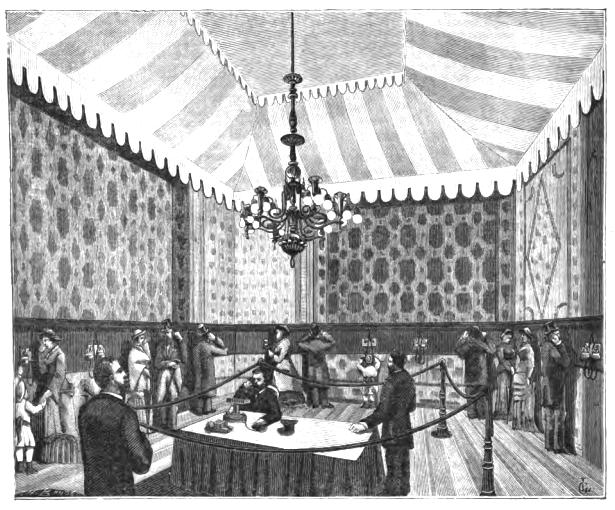
\includegraphics[width=1\columnwidth]{CAPITOLI/1000/IMG/1881opr4.jpg}
\caption{Illustrazione della sala d'ascolto del telefono all'Esposizione di
Parigi del 1881. Gli ascoltatori avevano i ricevitori telefonici per entrambe
le orecchie per ascoltare il programma teatrale in stereo.}
\label{fig:teatrophone2}
\end{figure}

Nonostante il telefono fosse un'invenzione giovanissima, al punto da pensare che
la diffusione del suono dal teatro alla sala d'ascolto avrebbe rappresentato
motivo di interesse da parte del pubblico a prescindere dalla condizionen di
ascolto, Ader aggiunse l'idea di esperienza che, attraverso i concetti di
binauralità e stereofonia, ebbe un impatto incredibile sul pubblico. L'articolo
comparso su \emph{L'Electricien} in cui si descrive il funzionamento
dell'invenzione fu firmato da M. Hospitaller che descrive così l'esperienza di
ascolto:

\begin{figure}[t]
\centering
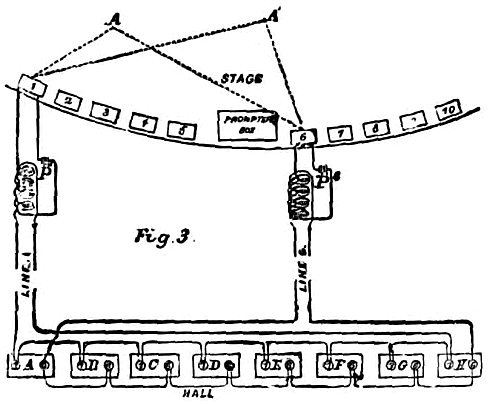
\includegraphics[width=1\columnwidth]{CAPITOLI/1000/IMG/1881opr2.jpg}
\caption{Disposizione dei trasduttori sul palco e collegamento alle due linee
telefoniche. Ogni ascoltatore è posizionata di fronte ad una coppia di telefoni
i quali ricevono il segnale da due trasduttori distinti posizionati sul palco.
Questi trasduttori sono raggruppati in coppie forniscono segnale a sedici
telefoni, accoppiati per otto ascoltatori.}
\label{fig:teatrophone1}
\end{figure}

\begin{quote}
We will now consider the new acoustic effect which Mr. Ader has discovered, and
applied for the first time in the telephonic transmission at the Electrical
Exhibition. Every one who has been fortunate enough to hear the telephones at
the Palais de l'Industrie has remarked that, in listening with both ears at the
two telephones, the sound takes a special character of relief and localization
which a single receiver cannot produce. [\ldots] As soon as the experiment
commences the singers place themselves, in the mind of the listener, at a fixed
distance, some to the right and others to the left. It is easy to follow their
movements, and to indicate exactly, each time that they change their position,
the imaginary distance at which they appear to be. [\ldots] This phenomenon is
very curious, it approximates to the theory of binauriclar auduition, and has
never been applied, we believe, before to produce this remarkable illusion to
which may almost be given the name of auditive perspective. [\ldots] In order
to realize it, we may recall the stereoscope, which allows us to see objects in
their natural relief\footnote{
\emph{Scientific American}, December 31, 1881, pages 422-423,\\
\url{https://earlyradiohistory.us/1881opr.htm} \\
Considereremo ora il nuovo effetto acustico che il signor Ader ha scoperto e
applicato per la prima volta nella trasmissione telefonica all'esposizione
elettrica. Tutti coloro che hanno avuto la fortuna di ascoltare i telefoni al
\emph{Palais de l'Industrie} hanno osservato che, ascoltando con entrambe le
orecchie ai due telefoni, il suono assume un carattere speciale di meraviglia e
localizzazione, cosa che un singolo ricevitore non può produrre. [\ldots] Non
appena inizia l'esperimento, i cantanti si posizionano, nella mente
dell'ascoltatore, a una distanza fissa, alcuni a destra e altri a sinistra. È
facile seguire i loro movimenti e indicare esattamente, ogni volta che cambiano
posizione, la distanza immaginaria alla quale sembrano essere. [\ldots] Questo
fenomeno è molto curioso, si avvicina alla teoria dell'audizione biauricolare che
crediamo non sia mai stato applicato prima di produrre questa straordinaria
illusione, a cui potrebbe essere dato il nome di prospettiva auditiva. [\ldots]
Per realizzarlo, possiamo ricordare lo stereoscopio, che ci consente di vedere
gli oggetti nel loro rilievo naturale.}.
\end{quote}

Tra le varie definizioni di stereofonia il termine è inoltre usato per indicare
la parte dell’acustica fisiologica che si occupa del fenomeno dell'ascolto
biauricolare del sistema uditivo. Tale fenomeno conferisce alla percezione umana
il potere localizzatore, cioè la capacità, dovuta al lavoro congiunto dei due
sistemi auricolari separati ed al sistema nervoso centrale, di determinare la
direzione di provenienza di un suono. In tal senso, esiste in acustica
fisiologica la definizione di monofonia in qualità di condizione anomala del
sistema percettivo, caratterizzata dalla mancanza degli elementi necessari a
individuare i caratteri spaziali dei suoni stessi, come per esempio quella
ottenuta con un solo orecchio.

La percezione dei caratteri spazio-temporali dei suoni, in particolare della
loro direzione di provenienza e della loro relazione con lo spazio che
attraversano, definiscono i tratti essenziali della stereofonia, in relazione
all'udito, in virtù dell’audizione biauricolare (o binaurale).

\begin{quote}
When recording music considerable trouble is experienced with the unpleasant
effects produced by echoes wich in the normal way would not be noticed by anyone
listening in the room in which the performance is taking place.
An observer in the room is listening with two ears, so that echoes reach him
with the directional significance which he associates with the music performed
in such room. He therefore discount these echoes and psychologically focuses
his attention on the source of the sound. When the music is reproduced through
a single channel the echoes arrive from the same direction as the direct sound
so that confusion results. [\ldots] Human ability to determine the direction
from which sound arrives is due to binaural hearing, the brain being able to
detect differences between sound received by the two ears from the same source
and thus to determine angular directions from which various sounds
arrive\footnote{[\cite{ab58}] - Quando si registra musica acustica, si riscontrano
notevoli problemi a causa degli effetti indesiderati prodotti dalle riflessioni
acustiche dell'ambiente, che nell'ascolto normale non vengono notati dagli
ascoltatori nella stanza in cui si svolge l'esibizione.
Un osservatore nella stanza sta ascoltando con due orecchie, in
modo che gli echi lo raggiungano con il significato direzionale che associa alla
musica eseguita in quella stanza. Pertanto, non tiene conto di questi echi e
focalizza psicologicamente la sua attenzione sulla fonte del suono. Quando la
musica viene riprodotta attraverso un singolo canale, gli echi arrivano dalla
stessa direzione del suono diretto, in modo da creare confusione. [...] La
capacità umana di determinare la direzione da cui proviene il suono è dovuta
all'udito binaurale, il cervello è in grado di rilevare le differenze tra il
suono ricevuto dalle due orecchie dalla stessa fonte e quindi di determinare le
direzioni angolari da cui provengono i vari suoni.}.
\end{quote}

È con queste parole che Blumlein nel 1931 descriveva i fondamenti delle conoscenze
in termini di percezione dei suoni e di come questi venivano utilizzati per definire
criteri tecnologici adeguati per la riproduzione dei suni. Ed è per questo che
in maniera piuttosto discreta intitola testo del brevetto che ha dato la nascita
commerciale e tecnologica alla stereofonia \emph{Miglioramenti in, ed in relazione,
ai sistemi di trasmissione del suono, registrazione del suono e riproduzione del suono}.
Genrico, inglese, la binauralità dell'ascolto umano è la prima affermazione di
Blumlein: “\emph{un osservatore nella stanza sta ascoltando con due orecchie}”.
Come questa condizione di ascolto si evolva nel tempo è la peculiarità della
stereofonia.

Il documento presenta diverse tecniche stereofoniche di microfonazione, di
incisione del disco e di trasmissione radio. La domanda fu presentata nel
dicembre 1931 ed approvata nel giugno 1933. Nel testo fa riferimento al cinema,
consapevole della necessità di migliorare la resa della registrazione sonora
in situazioni di “realismo”.

\emph{Una voce in una piccola stanza riverberante è una condizione d'ascolto che
rispetti qualità di stereofonia?}

In funzione di dei riferimenti storici e delle descrizioni fatte finora, la
risposta è chiaramente affermativa. Anche con un solo oggetto sonoro, una sola
voce, in una piccola stanza, siamo in presenza di un fenomeno acustico
stereofonico, percepito bianuralmente. Su questa condizione Blumlein presenta
le basi teoriche e tecnologiche della stereofonia, nel brevetto in cui ne
rende i concetti fondamentali, solidi, stabili nel tempo e nello spazio delle
parole.


%%%%%%%%%%%%%%%%%%%%%%%%%%%%%%%%%%%%%%%%%%%%%%%%%%%%%%%%%%%%%%%%%%% SECTION FOUR
%%%%%%%%%%%%%%%%%%%%%%%%%%%%%%%%%%%%%%%%%%%%%%%%%%%%%%%%%%%%%%%%%%%%%%%%%%%%%%%%
\section{Ramificazioni}

Con la profonda conoscenza del significato del tempo tra noi e Blumlein,
possiamo esporre il significato degli altoparlanti meglio di lui. Per l'era
Blumlein, l'altoparlante era lo strumento futuro per un tempo presente migliore.
Il suono riprodotto, alla sua giovane età, era pura magia. Oggi sappiamo bene
quanto siamo insoddisfatti della riproduzione degli altoparlanti. Quando il
primo iPhone è stata l'unica cosa intelligente sul pianeta, è stato fantastico,
un fantastico oggetto di creazione. Oggi con lo stesso oggetto non faremmo
nemmeno una foto. Ascoltare un assolo di violino riprodotto dal miglior
altoparlante sul mercato non è la stessa esperienza della performance reale.
Non è legato alla stereofonia e all'abilità tecnica, è parte integrante del
limite di riproduzione della tecnologia che siamo in grado di realizzare.
%
Sostituendo la voce umana che parla dell'esempio precedente, con un singolo
altoparlante che parla delle registrazioni di quella voce umana perdiamo, come
descritto da Blumlein, la capacità delle orecchie-cervello decifra la relazione
suono-ambiente. Non è più lo stesso ascolto stereofonico. Il numero di fonti è
lo stesso. Entrambi nel loro linguaggio monofonico producono una diversa
condizione di ascolto.%

Nel 1992 Michael Gerzon \cite{mg92pdmsss} disegna una rappresentazione
schematica delle diverse posizioni degli altoparlanti per stereo multispeaker,
da una a cinque:

\begin{quotation}
\ldots we show the loudspeaker layouts considered for frontal stage stereo
using from one (regarding mono as the trivial case of “one-loudspeaker stereo”!)
to five loudspeakers…
\end{quotation}

Esiste una condizione stereo con un solo altoparlante? Davvero si.

Un altoparlante in grado di suonare se stesso, non riproducendo qualcosa di
reale acustico ma producendo un suono che non potrebbe vivere senza un
altoparlante, rappresenta una condizione stereo con caratteristiche generali
simili alla voce parlante. Un rumore rosa filtrato da Butterworth che canta
monofonicamente in una stanza è una condizione di stereofonia.

Per un musicista elettroacustico, gli altoparlanti sono strumenti. La scelta
degli altoparlanti, la conoscenza del loro carattere e delle loro
caratteristiche è un momento necessario per quel musicista. Conoscere il loro
personaggio richiede tempo. Cambiare manualmente la frequenza di un suono
sinusoidale riprodotto da un altoparlante a tre vie, a un metro di distanza,
con le orecchie alla stessa altezza del centro dell'altoparlante, è un buon modo
per dire Ciao! all'altoparlante. Il musicista scoprirà in questo modo che i
suoni prodotti dall'altoparlante cambieranno forma durante lo spazzamento. Forse
vicino al punto di incrocio del crossover troverà alcune peculiarità, altre
strane decorrelazioni di fase ad altissima frequenza. Gli altoparlanti sono
strumenti. Due altoparlanti potrebbero essere il minimo impostato per la
condizione stereofonica di ascolto. Potrebbero essere cantanti elettroacustici
polifonici. Potrebbero anche essere una condizione monofonica, quando non sono
richieste stereofonia o polifonia.%

\begin{figure}[h]
\begin{center}
  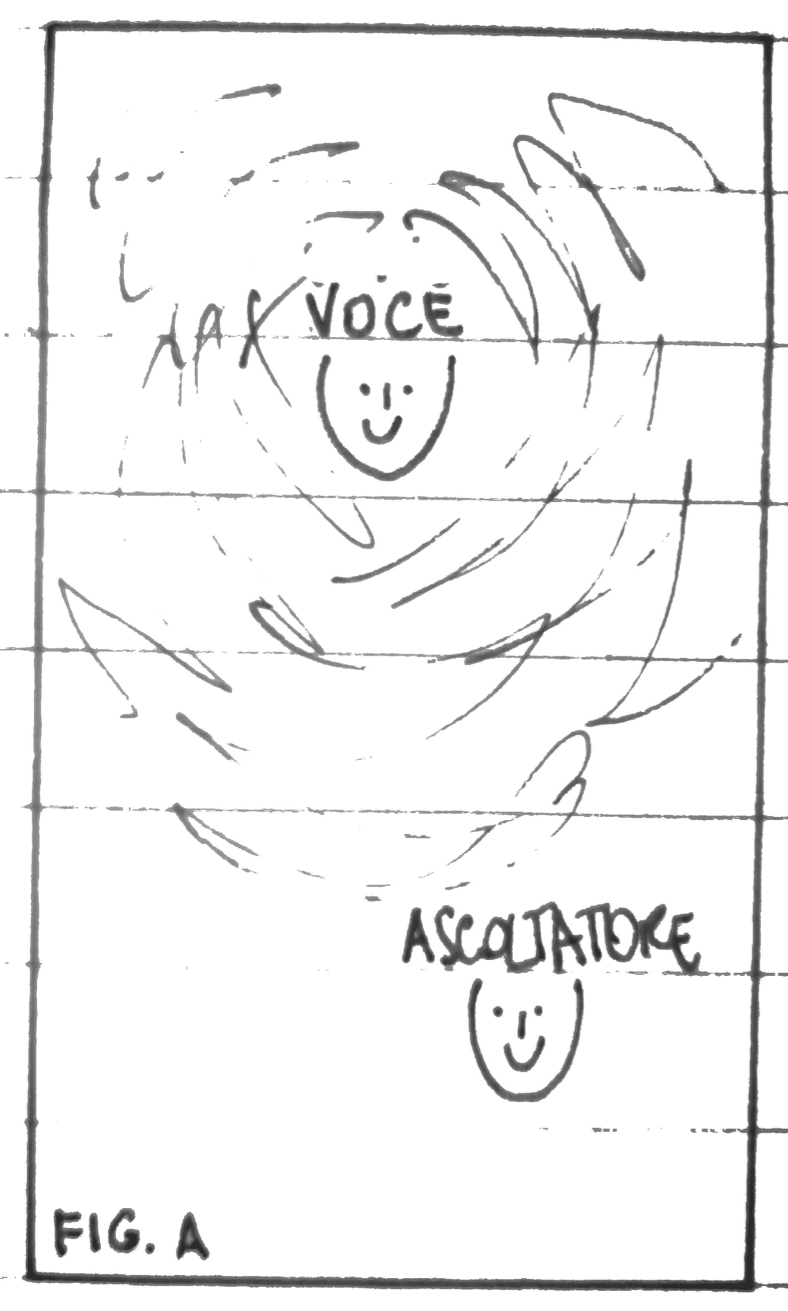
\includegraphics[width=.48\linewidth]{CAPITOLI/1000/IMG/figa.png}
%\caption{}
\label{ee:figa}
\end{center}
\end{figure}

Una voce nello spazio di una stanzetta si dirige, con una sua direzione, verso
un punto e contemporaneamente, con meno direzionalità, lateralemente, raggiunge
il resto della stanza. Questo meccanismo ha a che fare con la forma sonora di una
voce, prima ancora che con la forma architettonica della piccola stanza.

Dobbiamo immaginare la forma sonora come un'armatura attorno al nostro oggetto
sonoro, un'armatura fatta di fittissime molecole in vibrazione. Ogni suono ha una
sua veste plastica. Se vi dicessi ottavino e poi contrabbasso voi avreste già
collegato tutto ciò che vi serve per vederli, sentirli, ed ora, volendo, vestirli
della loro forma sonora. Ma cosa accade alla forma sonora di uno strumento in
presenza di tecninche estese applicate allo strumento? Una mano che inizia a produrre
suono li, nello stesso luogo dello strumento, a dove pochi minuti prima premeva
solo tasti (la mano  sinistra di UR) diventa esplosione di forma acustica e musicale.

Ecco questo è un po' il cuore di quello che vorrei fosse il mio dottorato di
ricerca che non avrò mai e un po' anche la manifestazionne di una piuttosto
triste verità: esclusi i percorsi individuali e rari percorsi di ricerca
non istituzionalizzata, la musica contemporanea ha esaurito la sua carica
contributiva al conoscimento, alla comprensione generalizzata.

Tornando alla forma, Questa si staglia nello spazio circostante e si espande e si muove
all'interno di questo spazio e ne viene modellata come una massa morbida all'interno
di un contenitore. Qui iniziano i fenomeni di riflessione e la forma si
cristallizza assumendo caratteristiche in funzione dello spazio e, quindi, del tempo.
L'ascoltatore che partecipa a questo evento vede una persona solida parlare nello
spazio di una stanza e sente la forma solida della voce provenire dalla sua bocca
e contemporaneamente, quindi subito dopo, dalla stanza sotto forma di riflessioni.
Sì! converremo infine, questa esperienza di ascolto rispetta queste qualità.

\begin{figure}[h]
\begin{center}
  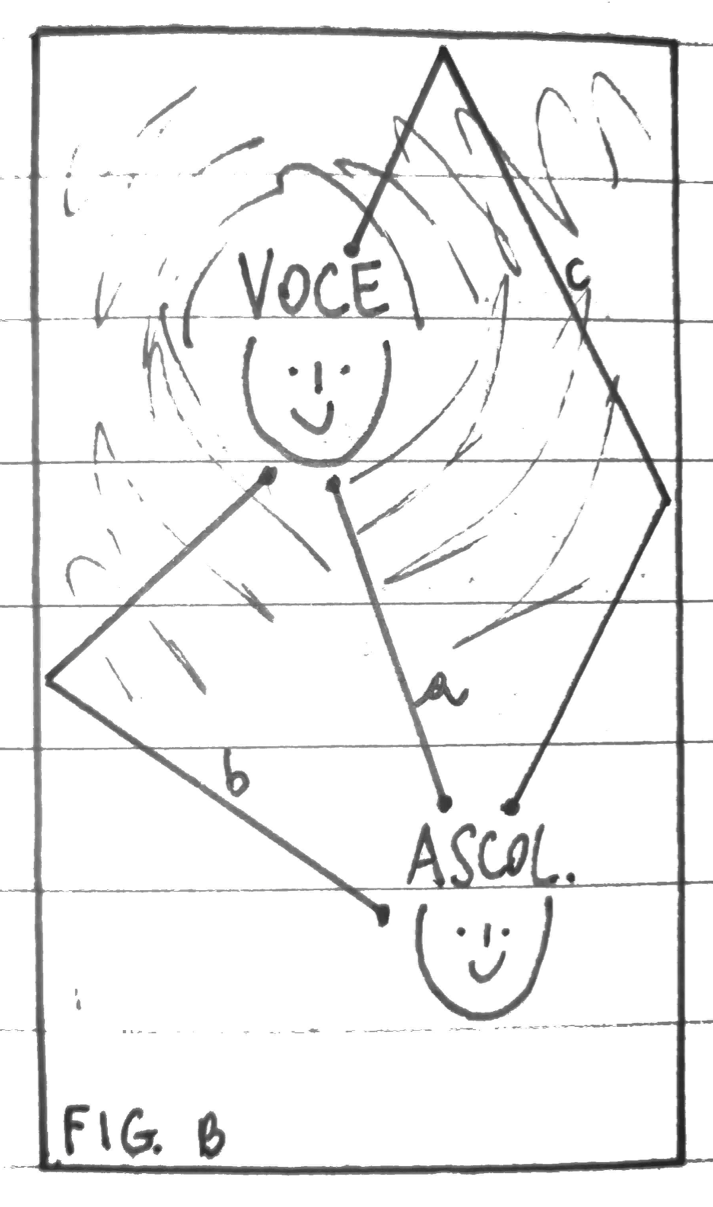
\includegraphics[width=.48\linewidth]{CAPITOLI/1000/IMG/figb.png}
%\caption{}
\label{ee:figb}
\end{center}
\end{figure}

Una voce che attraverso la sua forma acustica riempia uno spazio acustico è
un'esperienza d'ascolto stereofonica. Non è ancora giunto il momento di
interrompere la discussione dicendo: “ma come, non servono due diffusori?” Non
ancora, il problema è più complesso. È importante sottolineare che la stereofonia,
l'ascolto stereofonico, è una qualità dell'ascolto che si può osservare in
determinate circostanze e che richiede necessariamente il lavoro concertato delle
due orecchie. Un ascolto stereofonico è quindi possibile solo in coincidenza
con un ascolto \emph{binaurale}, ovvero effettuato con entrambe le orecchie.

Di nuovo una qualità che presuppone dei contenuti coerenti con delle
caratteristiche specifiche. Ora, nel mondo elettroacustico, del suono prodotto
o riprodotto elettricamente, dovremmo essere in grado di effettuare lo stesso
ragionamento sostituendo alla persona che parla un diffusore generico. Come per
l'essere umano, la voce è esempio di suono proprietario anche per il diffusore
si può scegliere un suono che lo caratterizzi elettroacusticamente, un suono
che lo rende particolare: il suono definito rumore rosa. Posizionato il diffusore
nella stessa stanza e con le stesse circostanze di ascolto precedenti, avremmo
una condizione di ascolto stereofonico? Ovviamente si. Un solo diffusore può
costituire una condizione d'ascolto stereofonica. In questo caso l'oggetto
acustico è un diffusore che esprime se stesso attraverso un suono non informativo.
Un rumore è caratterizzato da un'assenza di informazione, fatta esclusione del
fatto stesso che è rumore.

\begin{figure}[h]
\begin{center}
  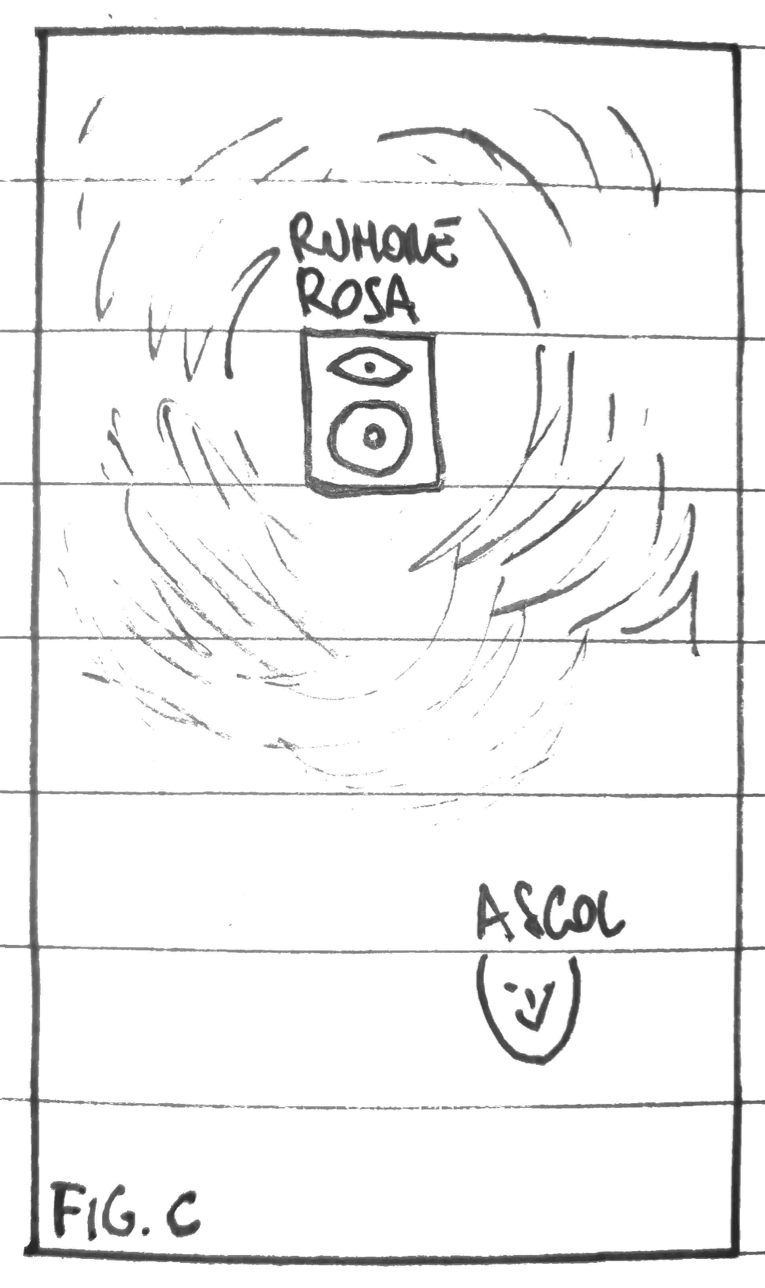
\includegraphics[width=.48\linewidth]{CAPITOLI/1000/IMG/figc.png}
%\caption{}
\label{ee:figc}
\end{center}
\end{figure}

che informazioni? be quelle che descrivono un suono come la percezione di altezza,
durata, intensità e timbro. Questa descirizione di stereofonia possibile anche
con un solo soggetto sonoro, voce o diffusore che sia, non è così comune e
condivisa. Ciò accade a causa del fatto che spesso si fa confusione tra stereofonia,
o stereofonica, come aggettivo applicato alla tecnica di diffusione e registrazione
piuttosto che alla qualità percettiva che queste tecniche dovrebbero suggerire.

Per arrivare a descrivere la tecnica dobbiamo percorrere ancora alcuni passi.

Nel momento in cui si passa da un dominio puramente acustico sia esso derivante
da una voce umana quanto un rumore diffuso attraverso un altoparlante, ad un
dominio di riproduzione acustica, ovvero di rappresentazione attraverso meccanismi
e tecniche allora cambia completamente lo scenario acustico e le circostanze di
ascolto. Un diffusore tradizionale può riprodurre una voce umana o un diffusore
che suona rumore rosa? Si certo che può riprodurli. Questa riproduzione
costituirebbe un ascolto stereofonico della sorgente originale? No, non lo sarebbe.

\begin{figure}[h]
\begin{center}
  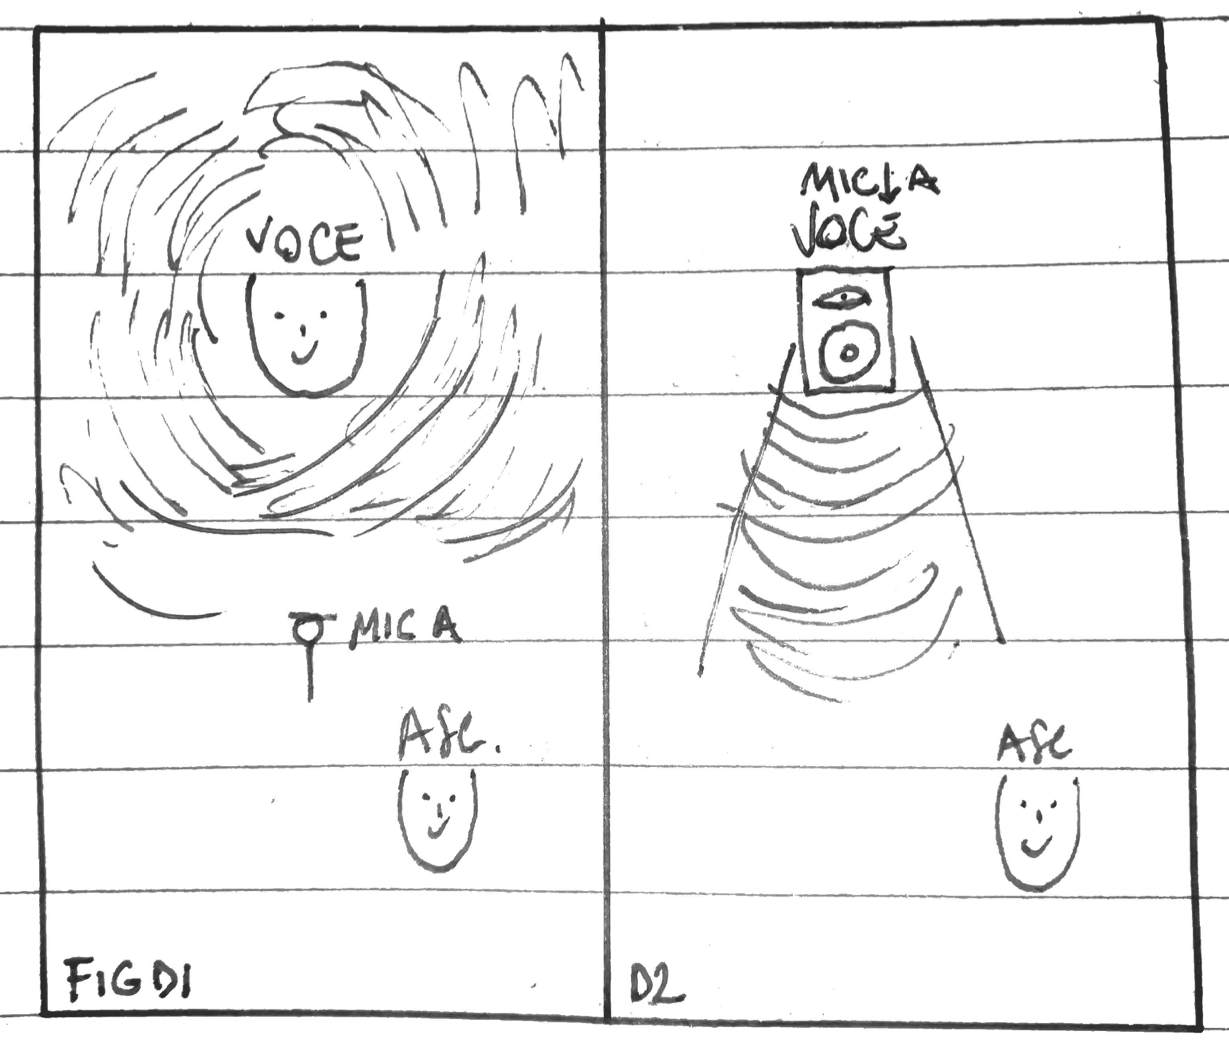
\includegraphics[width=.98\linewidth]{CAPITOLI/1000/IMG/figd1d2.png}
%\caption{}
\label{ee:figd1d2}
\end{center}
\end{figure}


\begin{quote}
When the music is reproduced through a single channel the echoes arrive from the same direction as the direct sound so that confusion result\footnote{Quando la musica viene riprodotta attraverso un singolo canale, gli echi arrivano dalla stessa direzione del suono diretto in modo tale da creare confusione.}.
\end{quote}

Qui si sviluppa tutta la questione, un solo diffusore non è in grado di rappresentare
la solidità originaria, la forma sonora dell'oggetto acustico originario, il suo
rapporto con lo spazio che lo ha modellato. Per comprendere meglio ogni possibile
questione legata alla diffusione sonora, mediante dispositivi elettroacustici ci
vorrebbe un minimo di tempo speso nella sperimentazione con lo strumento altoparlante.
Perché di questo si parla, di uno strumento tecnico, tecnologico, musicale e
profesisonale.

\begin{quote}
Ci sono problemi che alle volte anch'io non capisco, nel senso che se ne porgono
continuamnte di nuovi. È da anni che lavoro e sperimento negli studi di live electronics di
Friburgo, della Sudwestfunk. Si tratta delle trasformazioni in tempo reale del
suono e della voce, e del comporla con lo spazio, usando le tecnologie di oggi,
con i vari altoparlanti disposti nella sala. C'è qualcosa di nuovo solo sul piano
tecnico, perché  se prendiamo la Scuola di S. Marco veneziana di Andrea e Giovanni
Gabrieli, Monteverdi, di Willaert, con le composizioni a più cori, la grande
scuola spagnola all'epoca di Filippo II [\ldots] si faceva musica per otto organi
e quattro cori, cioè si suonava lo spazio come componente musicale, non come poi
la prassi dell'ottocento usa lo spazio, mettendo dentro l'orchestra e quel che
succede succede. Quindi altri studi, anche studi di fisica architettonica, studi
di processi di eco, di riverberazione, di materiali acustici. [\ldots] Qui una
composizione non è  data una volta per sempre, perché per ogni spazio noi dobbiamo
cambiare i programmi dei computer e modificando i rapporti della trasformazione si modifica anche il rapporto acustico; [\ldots] il grande fascino di questo per me
è veramente la non ripetitività. [\ldots] Un interprete non deve studiarsi la
parte ma veramente partecipare. [\ldots] Cioè vedi come noi possiamo con la
tecnologia di oggi studiare molto meglio, cioè studiare in un altro modo. \\
Luigi Nono 1986
\end{quote}

La parabola bacchiana si conclude con una nota autobiografica. Noi, che abbiamo
osservato da vicino la maledizione di Bacco, non possiamo più tacere e seminiamo,
il vento muoverà le orecchie penzolanti e porterà le nostre confessioni altrove.
%%%%%%%%%%%%%%%%%%%%%%%%%%%%%%%%%%%%%%%%%%%%%%%%%%%%%%%%%%%%%%%%%%%%%%%%%%%%%%%%%%%%%%%%%%%%%%%%%% fiune dalle esposizioni

Una singola voce umana, monofonica, sta parlando all'interno di una piccola
stanza, una condizione stereofonica accettabile? In accordo con Blumlein,
Sì! Questo è il primo punto fermo.

Michael Gerzon, dagli anni settanta agli anni novanta, dalle radici dell'era di
Blumlein ha saltato la linea con una dozzina di descrizioni chiare sulla
percezione e tentativi di progettare tecnologie di riproduzione per colmare il
divario rispetto al regno acustico.

\begin{quotation}
The ears and brain localize sounds according to many different mechanism. Among
the most important cues used are low frequency interaural phase (applicable up
to around 2\emph{KHz}, but dominant below 700\emph{Hz}) and localization by
amplitude differences between the two ears, predominantly above about
1\emph{KHz}. While other cues are also important, we have found that satisfying
both these cues, and making them mutually consistent for central listener facing
in any direction, leads to particularly robust and reliable localization
quality.\cite{mg92pdmsss}
\end{quotation}

%%%%%%%%%%%%%%%%%%%%%%%%%%%%%%%%%%%%%%%%%%%%%%%%%%%%%%%%%%%%%%%%%%%% SUBSECTION
%%%%%%%%%%%%%%%%%%%%%%%%%%%%%%%%%%%%%%%%%%%%%%%%%%%%%%%%%%%%%%%%%%%%%%%%%%%%%%%%
\subsection{Sul concetto di \emph{PanPot}}
\label{sec:panpot}

L'oggetto \emph{panner} è rappresentato da un potenziometro di controllo
(hardware o software, in entrambi i casi a controllo analogico o digitale) che
regola la distribuzione di un segnale su più canali componenti un campo sonoro
stereo o multicanale. Ogni mixer ha un \emph{panpot} (abbreviazione di
\emph{potenziometro di panoramica}), per ciascun canale sorgente in ingresso,
che regola l'azione del \emph{panner}.

%L'ultima precisazione riguarda il movimento panoramico. La distribuzione dell'energia
%o la condizione della coppia di segnali che regola il movimento panoramico troppo
%spesso sono descritti come la possibilità di muovere gli oggetti attorno alla posizione
%dell'ascoltatore.

Generalmente il \emph{panpot} viene descritto come un pomello che permette di
muovere i suoni tra la sinistra e la destra del panorama di diffusione, il che è
parzialmente vero e potenzialmente pericoloso in termini di immaginazione
acustica.

Soffermandosi ad analizzare il fenomeno acustico di un suono prodotto da un
oggetto in movimento tra la destra e la sinistra di un campo percettivo emergono
diversi problemi.

Il primo riguarda l'\emph{effetto doppler}. Siamo seduti su una panchina al
margine di una strada che si estende infinita agli estremi della nostra vista
periferica. Un mezzo di soccorso, con la sirena accesa, si avvicina percorrendo
la strada davanti al nostro viso, da sinistra verso destra: percepiamo
una variazione in frequenza al passaggio della sirena, in funzione della
velocità. L'\emph{effetto doppler} ci descrive come nel percorso di
avvicinamento a noi la frequenza sale lentamente fino al massimo ottenuto nel
momento in cui ci raggiunge per poi diminuire rapidamente in coincidenza con
l'allontanamento.

Ora siamo dei \emph{sound designer}, siamo seduti di fronte alla nostra console
analogica e dobbiamo replicare l'effetto sopra descritto. Applicando un
movimento da sinistra a destra, azionando il \emph{panpot} su un suono di sirena
statico, registrato fermo ad un metro di distanza, pur ruotando velocemente il
potenziometro non otteniamo variazioni in frequenza. Il suono si muove tra la
sinistra e la destra del sistema d'ascolto senza produrre il movimento nello
spazio ma solamente lo spostamento della posizione relativa al nostro punto di
ascolto. Ne deriva una prima conslusione: il \emph{panpot} regola una posizione
relativa, non stabilisce criteri di movimento.

Un altro problema emergente del pensare il \emph{panning} come un movimento
scaturisce dalla relazione della sorgente con l'ambiente circostante. Che
movimento può esserci senza tenere conto del luogo in cui la sorgente sonora si
trova? Un avvocato pronuncia la sua arringa in tribunale parlando ad alta voce,
camminando, rimbalzando tra destra e sinistra. La voce si propaga nello spazio
ed è inevitabile che se ne percepisca la variazione topologica, morfologica in
relazione con le caratteristiche architettoniche: a sinistra della stanza c'è
una parete di finestre, a destra un muro in cemento. Pur non avendo velocità
sufficiente ad innescare l'effetto doppler, la sua continua variazione di
posizione corrisponde ad una continua variazione di rapporto con l'ambiente che
lo circonda, in relazione ad ogni infinto punto di ascolto all'interno della
stanza. In altre parole, quel movimento assume significati diversi relativi al
punto di ascolto.

Dovendo simulare lo stesso effetto mediante l'azione sul panpot, otterremmo la
variazione di posizione della voce nello spazio, ma non la sua relazione con lo
spazio.

\begin{figure*}[t!]
    \centering
    \begin{subfigure}[t]{0.45\textwidth}
        \centering
        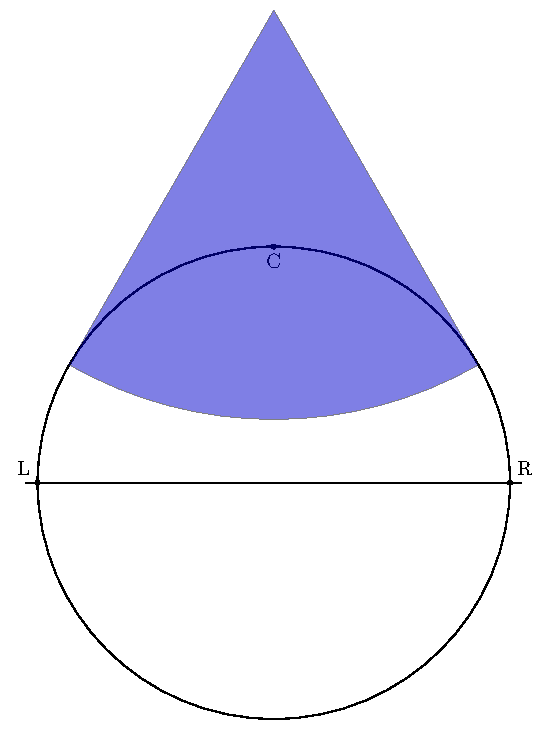
\includegraphics[height=8cm]{CAPITOLI/_TIKZ/PANNING/pan-frontal}
        \caption{Sorgente con incidenza frontale.}
        \label{pan:frontal}
    \end{subfigure}%
    ~
    \begin{subfigure}[t]{0.45\textwidth}
        \centering
        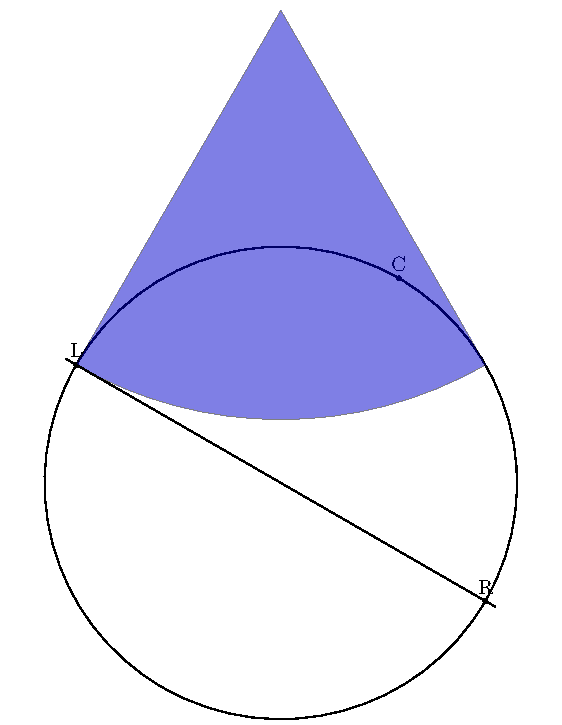
\includegraphics[height=8cm]{CAPITOLI/_TIKZ/PANNING/pan-left}
        \caption{Sorgente con incidenza laterale sinistra di 30 gradi.}
        \label{pan:left}
    \end{subfigure}
    \\
    \begin{subfigure}[t]{0.9\textwidth}
        \centering
        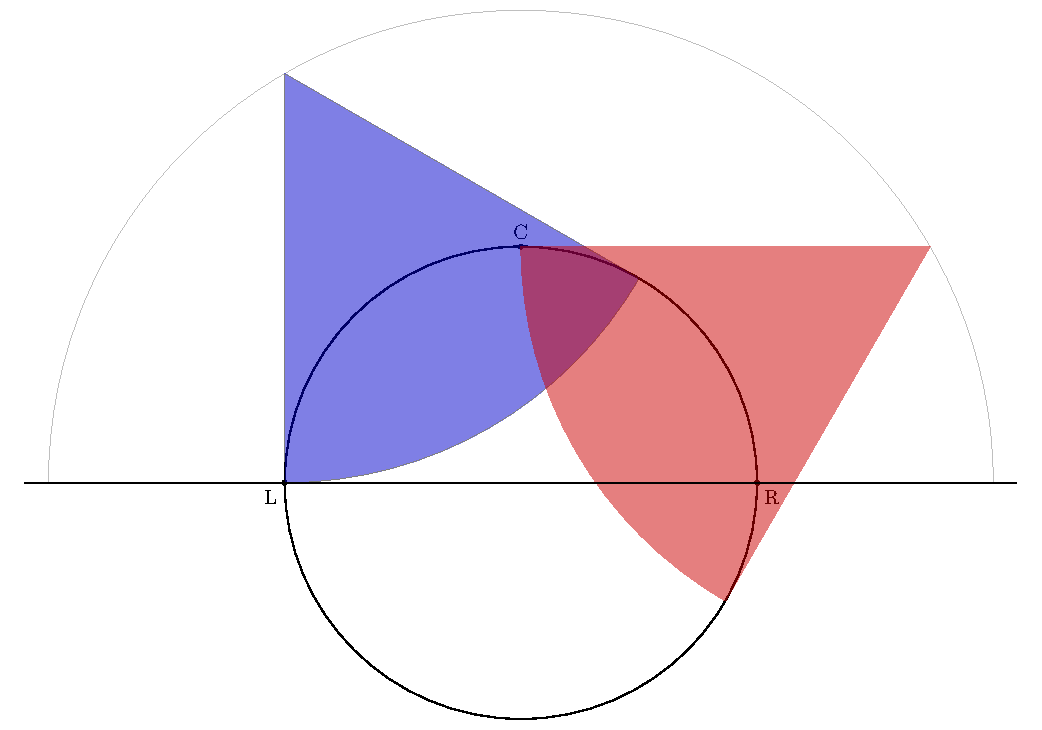
\includegraphics[height=8cm]{CAPITOLI/_TIKZ/PANNING/pan-both}
        \caption{Due sorgenti, una con incidenza laterale sinistra di 30 gradi,
        l'altra con incidenza laterale destra di 60 gradi.}
        \label{pan:both}
    \end{subfigure}
    \caption{La rotazione del \emph{PanPot} esegue una modifica della condizione
    di ascolto dell'ascoltatore, non un movimento della sorgente. Posizionando
    le singole sorgenti ci si pone in ascolto laterale, ruotati. Nella
    sovrapposizione di molteplici sorgenti il panorama risulta composto da
    ognuna di queste, con posizioni assolute ed angoli di incidenza relativi
    della testa.}
    \label{pan:all}
\end{figure*}

Il \emph{panpot}, nella sua capacità di descrizione della relazione tra i canali
che ricevono i suoi segnali, non muove la sorgente nello spazio, ma regola la
posizione della sorgente stessa in relazione al nostro punto di ascolto. In
altri termini il \emph{panner} non regola il movimento della sorgente, ma la
rotazione della testa in relazione ad essa. Il \emph{panner}, muove langolo di
incidenza del suono, ruota la testa, nei confronti della sorgente immobile.

Ogni \emph{panner} ha un'architettura interna che determina la quantità e la
condizione del segnale sorgente per ogni canale di destinazione. I più semplici
suddividono i segnali audio nei due canali sinistro e destro, attraverso un
opportuno controllo di guadagno (volume) discreto. La distribuzione dell'energia
tra i due canali è chiamata legge ed è descrivibile con una funzione matematica.

Come descritto da Blumlein, la sola variazione di ampiezza nella
rappresentazione del panorama stereofonico rappresenta una parte nella complessa
soddisfazione della percezione binaurale, non disegna l'intero meccanismo.
Per questo motivo, prima di descrivere i sistemi di panning di ampiezza, che
sono universalmente implementati su tutti i mixer del pianeta, è più opportuno
riprendere da dove egli stesso è partito. La visione di Blumlein fu ripresa in
seguito da Michael Gerzon, negli anni settanta, per sviluppare la tecnologia
\emph{ambisonic}, la quale rimane un atto di descrizione del mondo sonoro
percepito e riprodotto, nell'evoluzione della stereofonia, completamente diverso
da quello che commercialmente si è diffuso ed imposto.

%%%%%%%%%%%%%%%%%%%%%%%%%%%%%%%%%%%%%%%%%%%%%%%%%%%%%%%%%%%%%%%%%%%% SUBSECTION
%%%%%%%%%%%%%%%%%%%%%%%%%%%%%%%%%%%%%%%%%%%%%%%%%%%%%%%%%%%%%%%%%%%%%%%%%%%%%%%%
\subsection{Sul concetto di \emph{Diagramma Polare}}
\label{sec:polarplot}

Il diagramma polare (o curva polare) è invece un grafico a disegno circolare
dove i parametri sono dati dall’ampiezza e dall’angolo d’incidenza, mentre le
frequenze sono rappresentate da famiglie di curve. In presenza di un’unica curva,
si intende che questa è riferita ad una frequenza di $1KHz$. %piero

Un singolo segnale, nella sua oscillazione, espressa nella variazione di ampiezza
attorno allo zero, potrebbe essere derivato da qualsiasi tipo di microfono senza
un significato particolare. Potrebbe essere generato elettricamente da un
microfono con modello polare particolare o da una fonte sintetica senza
alcuna rilevanza specifica. La provenienza polare, la forma che assume la fase
del segnale, diventa rilevante nel confronto tra segnali.

Il diagramma polare di un microfono che, per caratteristiche costruttive, non
percepisce variazioni di angolo di incidenza del segnale, quindi non-direzionale,
è definito comunemente come omnidirezionale, la sua equazione contiene solo
variazioni di ampiezza, derivate della variazione di pressione dell'aria

\begin{equation}
ndp = 1(x)
\label{eq:omni}
\end{equation}

\begin{figure}[h]
\centering
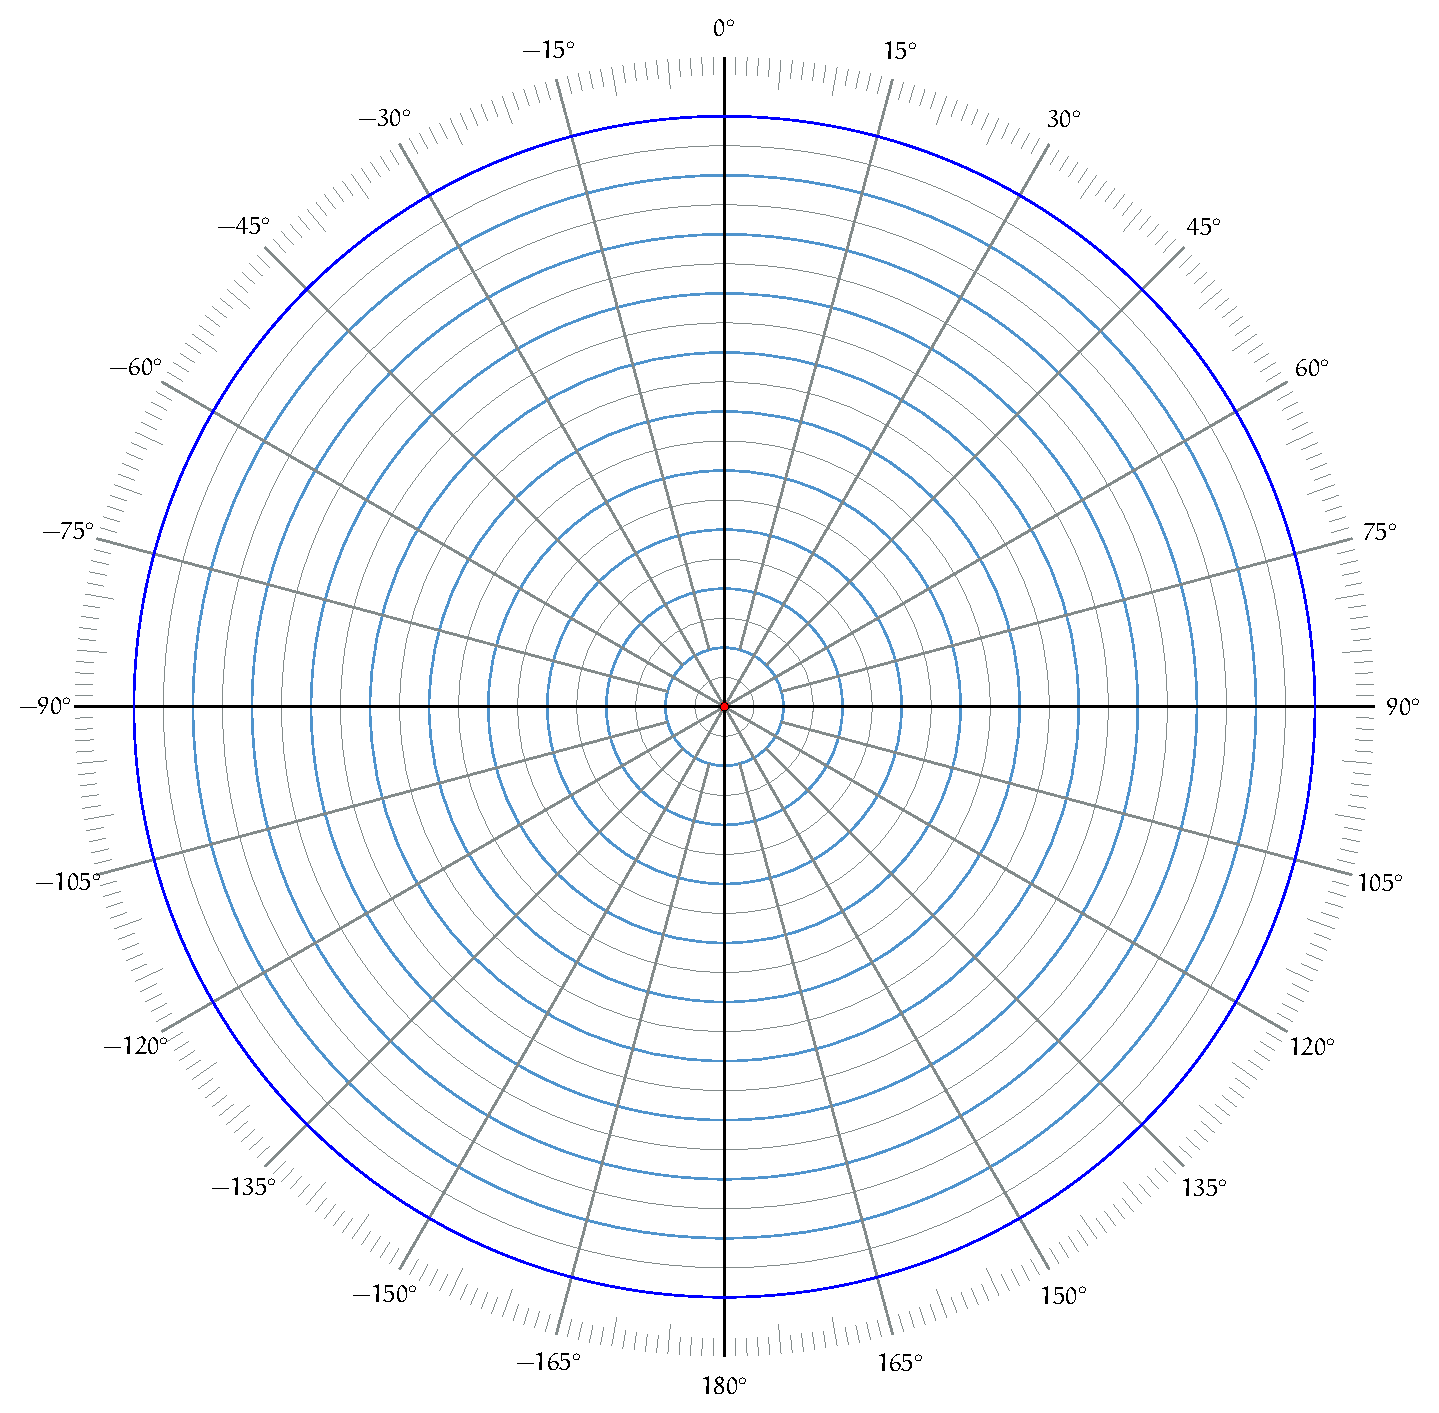
\includegraphics[width=1\columnwidth]{CAPITOLI/_TIKZ/POLAR/omni}
\caption{non-directional}
\label{polar:omni}
\end{figure}

%Il disegno nella parte sinistra di fig. 8 rappresenta la struttura di un tipico microfono a pressione (pressure microphone) omnidirezionale, mentre nella parte destra è rappresentata la sua curva polare, dove vediamo che la direzionalità del suono inizia ad essere percepita dal microfono a partire da circa 5 KHz in su, mentre le frequenze gravi non sono indicate in quanto assimilabili a quella rilevata a 1 KHz, cioè con attenuazione zero per qualsiasi angolo di provenienza del suono.


% %%%%%%%%%%%%%%%%%%%%%%%%%%%%%%%%%%%%%%%%%%%%%%%%%%%%%%%%%%%%%%%%% SECTION FIVE
% %%%%%%%%%%%%%%%%%%%%%%%%%%%%%%%%%%%%%%%%%%%%%%%%%%%%%%%%%%%%%%%%%%%%%%%%%%%%%%
\section{Mid-Side}
Harvey Fletcher, fisico americano, nel 1934 firma uno degli articoli che
compongono un testo cardine per la storia della tecnologia sonora
“\emph{Symposium on Auditory Perspective}”, sulla percezione e la trasmissione
della musica dal vivo, che inizia con le seguenti parole:

\begin{quote}
In this electrical era one is not surprised to hear that orchestral music can be
picked up in one city, transmitted a long distance, and reproduced in another.
Indeed, most people think such things are commonplace. They are heard every
night on the radio. However, anyone who appreciates good music would not admit
that listening even to the best radio gives the emotional thrill experienced in
the concert hall. \cite{hf34}
\end{quote}

Oggi abbiamo perso ogni scintilla di “quell'era elettrica”, anche quella che ha
suscitato la fiamma di interesse nell'ascolto della musica orchestrale
attraverso la trasmissione.

%, o quella che ha suscitato la fiamma di interesse
% nell'ascolto della musica orchestrale, o quella dell'interesse nell'ascolto o,
% molto più semplicemente, la fiamma dell'di interesse. Cento anni dopo quella
% “era” siamo scimmie. Dobbiamo considerare questo fallimento. Inadempienza. Dobbiamo considerare che
% un libro, anche il più inadeguato, in quanto oggetto di pensiero ha potere, come
% dimostrato nell'introduzione, che potrebbe essere il potere di distruggere.

Nel 1964, Paul W. Klipsch introdusse la ristampa del “\emph{Symposium}”:

\begin{quote}
The following paper is a reprint of one of the most important papers in the
field of audio. Fundamentals do not change. The laws of physics endure. In
reprinting the Symposium, the fundamentals are restated. \cite{sap1964}
\end{quote}

Il testo di Fletcher \cite{hf34} è datato 1934, un anno dopo l'approvazione
del brevetto Blumlein che descrive il concetto fondamentale di trasmissione e
registrazione del suono Mid-Side. In quell'epoca gli interessi commerciali e
quelli di ascolto erano intrecciati, in una forma \emph{stereo} solida.

Parlando di orecchie e attività cerebrali per determinare la direzione di una
fonte Blumlein ha scritto:

\begin{quote}
…it is fairly well established that the main factor having effect are phase
differences and intensity differences between the sounds reaching the two ears,
the influence with each of these has depending upon the frequency of the sounds
emitted. For low frequency sound waves there is little or non difference in
intensity at the two ears but there is a marked phase difference. For a give
obliquity of sound the phase difference is approximately proportional to
frequency, representing a fixed time delay between sound arriving at the two
ears, by noting which there is a phase difference of $\pi$ radians or more
between sound arriving at the two ears from a source located on the line joining
them: but above such frequency if phase difference were the sole feature relied
upon for directional location there would be ambiguity in the apparent position
of the source. At the stage however the head begins to became effective as a
baffle and causes noticeable intensity difference between the sounds reaching
the two ears, and it is by noting such intensity difference that brain
determines direction of sounds at higher frequencies\footnote{\cite{ab58} - ...è abbastanza
accertato che il fattore principale sia dovuto alle differenze di fase e di
intensità tra i suoni che raggiungono le due orecchie, l'influenza con ognuna di
queste differenze ha a seconda della frequenza dei suoni emessi. Per le onde
sonore a bassa frequenza c'è poca o nessuna differenza di intensità alle due
orecchie ma c'è una marcata differenza di fase. Per dare un'obliquità del suono,
la differenza di fase è approssimativamente proporzionale alla frequenza, che
rappresenta un ritardo fisso tra il suono che arriva alle due orecchie, notando
che c'è una differenza di fase di $\pi$ radianti o più tra il suono che arriva
alle due orecchie da una sorgente situata sulla linea che le unisce: ma al di
sopra di tale frequenza se la differenza di fase fosse l'unica caratteristica
su cui si basava per la posizione direzionale, ci sarebbe ambiguità nella
posizione apparente della sorgente. Tuttavia, nella fase in cui la testa inizia
a diventare efficace come un deflettore e causa una notevole differenza di
intensità tra i suoni che raggiungono le due orecchie, ed è notando tale
differenza di intensità che il cervello determina la direzione dei suoni a
frequenze più alte.}.
\end{quote}

Sulla base della conoscenza dei meccanismi sopra esposti Blumlein ha formulato
la maggior parte dei principi fondamentali impressi nella storia della stereofonia.
L'approccio più semplice descritto permette di ottenere semplici differenze di livello
nella riproduzione dagli altoparlanti, percepite come differenze di livello e di
fase dalle orecchie. Per ottenere questo tipo di segnale sono necessari almeno due microfoni
posizionati tra loro vicinissimi, allineati verticalmente, in modo da non avere alcun ritardo (orizzontale) tra i canali.
Questa configurazione definita \emph{coincidente} è l'ideale per alimentare
gli altoparlanti con differenze pure di ampiezza tra i canali. Una delle tipiche
tecniche di ripresa stereofonica per coppia coincidente prende proprio il nome
da Blumlein: due microfoni bidirezionali, figura-8 quindi a gradiente di pressione,
angolati tra loro di $\pm45$ gradi, in modo da avere un angolo retto tra loro.

Tuttavia, come esposto nel brevetto, i soli microfoni disponibili a Blumlein nei
suoi primi esperimenti erano non-direzionali a pressione. Coppie stereofoniche coincidenti
con microfoni di questo tipo non sono possibili, in quanto il loro allineamento verticale
produrrebbe due segnali identici, che non descriverebbero stereofonia. È necessaria
quindi una distanza tra i due microfoni. Due microfoni non-direzionali distanziati
anche poco tra loro sono in grado di produrre segnali quasi identici in ampiezza
ma diversi in fase. Blumlein quindi si concentra su una strategia per produrre
anche una differenza di ampiezza tra i due microfoni, inserendo un blocco di legno
tra i due microfoni e progettando una matrice elettrica che mettesse in
relazione i due segnali in modo da produrre le giuste differenze di ampiezza
nell'altoparlante. Il prodotto di tale ricerca fu la matrice di somma e differenza
alla base della tecnologia Mid-Side.

\begin{quote}
\ldots a system of sound transmission wherein the sound
is receive by two or more microphones, wherein at low frequencies difference in
the phase of sound pressure at the microphone is reproduced as difference in
volume at the loud speaker. [\ldots] two microphones transmitted over individual
channels are adapted to interact [\ldots] consisting in half of the sum and half
of the difference respectively of the original \cite{ab58}
\end{quote}

\begin{figure*}[b!]
    \centering
    \begin{subfigure}[t]{0.48\textwidth}
        \centering
        \includegraphics[height=6cm]{microphone-polar-patterns/xy90}
        \caption{Coppia stereofonica coincidente di cardioidi angolati di 90 gradi tra loro in entrata alla matrice.}% \\ Eq: $1(x)$}
        \label{pol:xy90ms}
    \end{subfigure}%
    ~
    \begin{subfigure}[t]{0.48\textwidth}
        \centering
        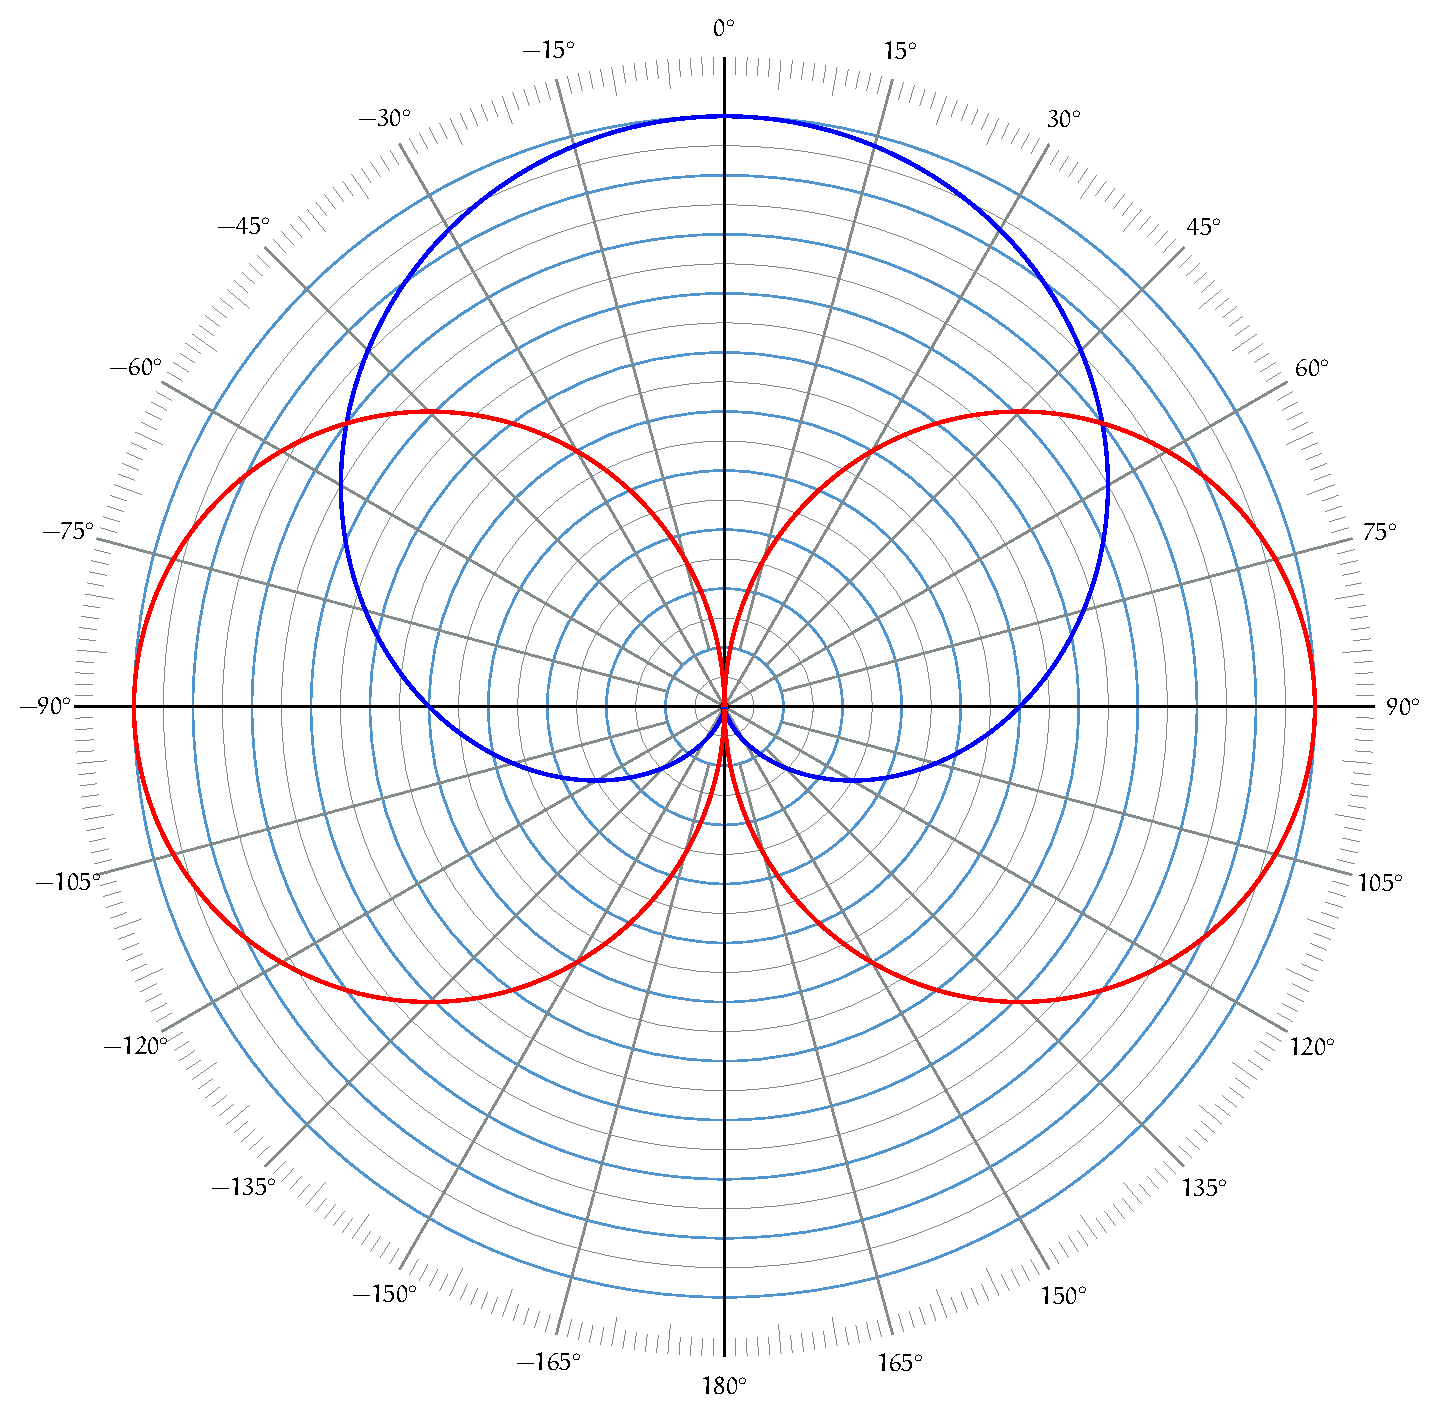
\includegraphics[height=6cm]{microphone-polar-patterns/midside}
        \caption{Le componenti \emph{Mid-Side} in uscita.}% \\ Eq: $0.75(x)+0.25(x\cos\theta)$}
        \label{pol:midsidems}
    \end{subfigure}
    \caption{Rappresentazione polare ideale del transito di una coppia \emph{xy90}
    attraverso la matrice e relativa rappresentazione d'uscita \emph{Mid-Side}.}
    \label{pol:msmatrix}
\end{figure*}

La matrice di Blumlein di somma e differenza tra i segnali è bidirezionale.
Quando il canale sinistro e destro di una coppia stereofonica passa attraverso la
matrice, la somma di entrambi i canali fornisce il segnale \emph{Mid} contenente solo le componenti in fase,
mentre la differenza produce il segnale \emph{Side} laterale contenente solo
componenti non in fase tra loro. Quando sono le componenti \emph{Mid-Side} a transitare
attraverso la matrice, la somma di \emph{Mid} e \emph{Side} fornisce la
correlazione tra fase sinistra e ampiezza, mentre la differenza produce la
correlazione tra fase negativa a ampiezza.

Di seguito il codice \emph{Faust} per la matrice somma e differenza.

%--------------------------------------------
%----------------larghezza massima del codice
\begin{lstlisting}
nsum = 0.5*(_+_);
ndif = 0.5*(_-_);
sdmx = _,_ <: nsum, ndif;
\end{lstlisting}

\begin{figure}[ht]
  \centering
  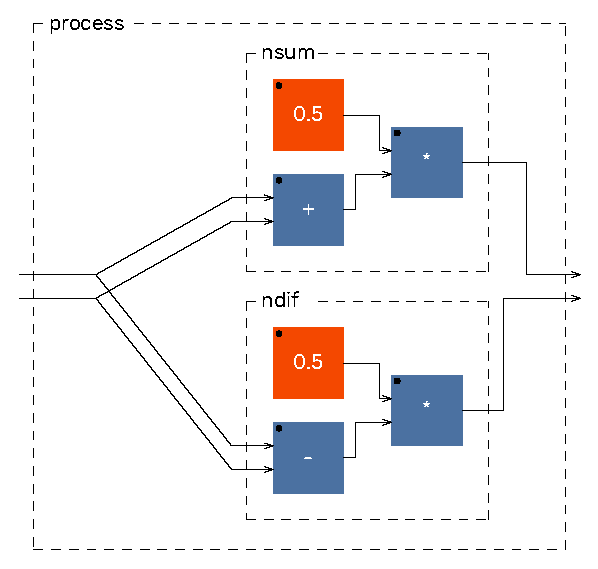
\includegraphics[]{CAPITOLI/1000/IMG/sdmx}
  \caption{Matrice somma e sottrazione.}
  \label{bd:sdmx}
\end{figure}

%%%%%%%%%%%%%%%%%%%%%%%%%%%%%%%%%%%%%%%%%%%%%%%%%%%%%%%%%%%%%%%%%%%% SECTION SIX
%%%%%%%%%%%%%%%%%%%%%%%%%%%%%%%%%%%%%%%%%%%%%%%%%%%%%%%%%%%%%%%%%%%%%%%%%%%%%%%%
\subsection{Mid-Side \emph{mic}}
\label{subsec:msmic}

\begin{figure}[b!]
\centering
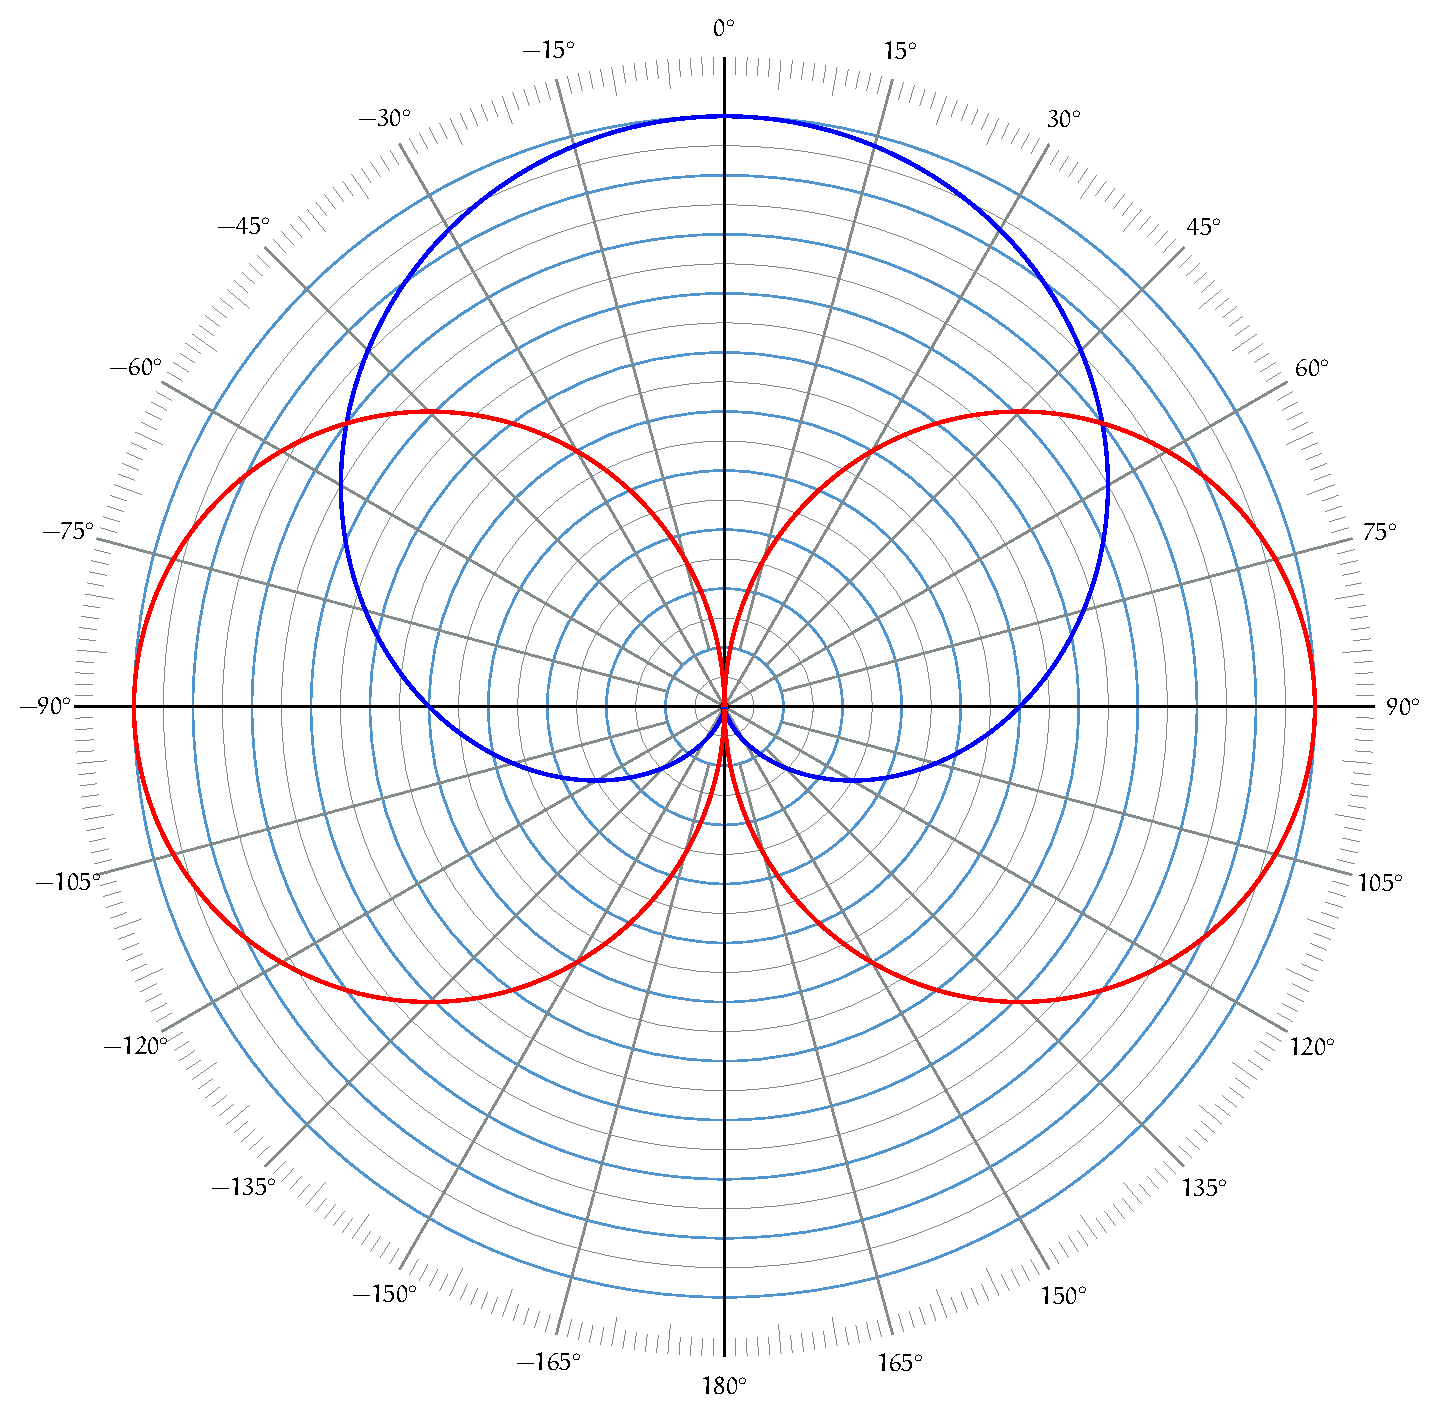
\includegraphics[width=0.99\columnwidth]{microphone-polar-patterns/midside}
\caption{Rappresentazione ideale della coppia stereofonica Mid-Side costituita da
da un microfono direzionale cardioide a gradiente di pressione mediante la sua
equazione polare: $cpg = 0.5(x) + 0.5(x\cos\theta)$ (\emph{cardioid pressure
gradient}) e da un microfono bidirezionale a gradiente di
pressione mediante la sua equazione polare: $bpg = x\cos\theta$
(\emph{bidirectional pressure gradient}). Nella tecnica microfonica di registrazione
Mid-Side il microfono cardioide convenzionalmente viene registrato nel primo canale,
mentre il segnale del microfono bidirezinale viene registrato nel secondo canale.}
\label{polar:midsidemic}
\end{figure}

La produzione di un segnale \emph{Mid-Side} come quello in uscita dalla matrice
somma e sottrazione può essere ottenuta dal posizionamento diretto di una coppia
di microfoni aventi caratteristiche polari adeguate. Il segnale \emph{Mid} è
generalmente prodotto da un microfono direzionale cardioide puntato verso il fronte
stereofonico, mentre il segnale \emph{Side} è generato da un microfono
bidirezionale puntato lateralmente, offrendo al fronte il punto di massimo
annullamento. I due microfoni devono essere allineati verticalmente in modo da
risultare orizzontalmente coincidenti.


%%%%%%%%%%%%%%%%%%%%%%%%%%%%%%%%%%%%%%%%%%%%%%%%%%%%%%%%%%%%%%%%%%%% SECTION SIX
%%%%%%%%%%%%%%%%%%%%%%%%%%%%%%%%%%%%%%%%%%%%%%%%%%%%%%%%%%%%%%%%%%%%%%%%%%%%%%%%
\subsection{Mid-Side \emph{panner}}
\label{subsec:mspanner}

La coppia stereofonica di segnali \emph{Mid-Side} è stata descritta finora come
risultante della matrice somma e sottrazione applicata ad un segnale stereofonico
oppure come segnale prodotto da una coppia di microfoni aventi caratteristiche
oppurtune. Analizziamo ora un terzo sistema in grado di generare una coppia
\emph{Mid-Side} attraverso un sistema di panning.

Il canale frontale \emph{Mid} è comunemente descritto da un microfono cardioide.
Sappiamo che la componente cardioide, come moltre altre figure polari, può
essere risultante da una combinazine misurata di
componenti non-direzionale e bidirezionale.

\begin{equation}
m(x,p,\theta) = (p*x) + ((1-p)*(x\cos\theta)
\label{eq:mid}
\end{equation}

Dove $x$ è il segnale di ingresso, $p$ è il coefficiente di ampiezza che regola
il rapporto di peso tra le due componenti, $0.5$ per ottenere la figura polare
cardioide, $\theta$ è la direzione di impatto angolare espressa in radianti.

La componente \emph{Side} è costituita dalla sola componente bidirezionale.

\begin{equation}
s(x,\theta) = x*(sin(\theta))
\label{eq:side}
\end{equation}

Il codice \emph{Faust} per la costruzione di un \emph{Mid-Side Panner} è
molto simile alle equazioni che descrivono le due figure polari.

%--------------------------------------------
%----------------larghezza massima del codice
\begin{lstlisting}
mspan(x,p,rad) = m,s
with{
  m = (p*x)+((1-p)*(x*cos(rad)));
  s = x*(sin(-rad));
};
\end{lstlisting}

I due segnali in uscita dal panner non possono essere inviati direttamente ad un
sistema di ascolto basato sui due canali sinistra-destra, devono necessariamente
passarli attraverso la matrice somma e differenza ottenere ciò che Blumlein
descrive come la differenza di ampiezza nei segnali degli altoparlanti
ottenuta dalle differenze di fase.

% %--------------------------------------------
% %----------------larghezza massima del codice
% \begin{lstlisting}
% mspan_lr(x,p,rad) = mspan(x,p,rad) : sdmx;
% \end{lstlisting}

\begin{figure}[t]
\centering
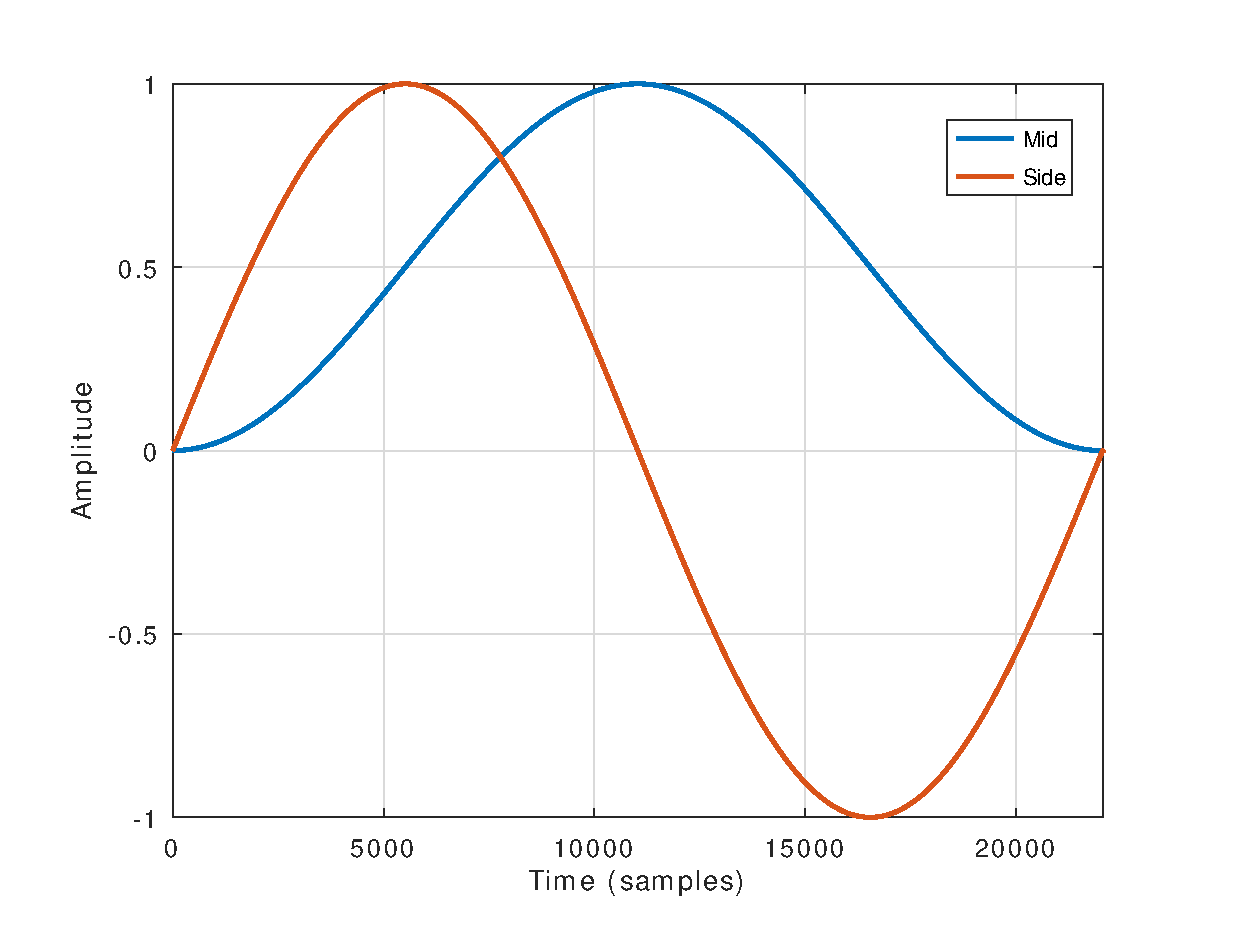
\includegraphics[width=0.99\columnwidth]{CAPITOLI/1000/IMG/mspan}
\caption{Mid-Side \emph{panner}. Il grafico mostra la risposta del \emph{panner} ad una
variazione di 360 gradi da sinistra (-180 gradi) a destra (180 gradi). La linea
rossa mostra la bipolarità del segnale correlata alle informazioni angolari. La
linea blu descrive variazioni di ampiezza (sempre con fase positiva) in
relazione alle informazioni angolari. Il grafico mostra l'evidenza della percezione
zero su entrambi gli estremi $\pm180$ gradi, dove cardioide e figura-8 si annullano.}
\label{fig:mspan}
\end{figure}

% La procedura di costruzione dell'algoritmo del \emph{Mid-Side Panner} è completa.
% Il seguente codice di \emph{Faust} descrivo il panner completo di interfaccia
% grafica.

%-----------------------------------------------------------
%-------------------------------larghezza massima del codice
\begin{lstlisting}
//----------------------------------- DEGREES TO RADIANS ---
deg2rad = *(ma.PI/180);
//----------------------------------------------- PANPOT ---
rad = vslider("[02]Azimuth[style:knob]", 0,-180,180,0.1) :
      deg2rad : si.smoo;
//--------------------------------------------- P FACTOR --–
p = vslider("[01]P[style:knob]", 0.5,0,1,0.01) : si.smoo;
//--------------------------------------------- MID-SIDE --–
midside(x,p,rad) = m,s
  with{
    m = (p*x)+((1-p)*(x*cos(rad)));
    s = x*(sin(-rad));
};
//-------------------------------- MS MATRIX DESCRIPTION ---
nsum = 0.5*(_+_);
ndif = 0.5*(_-_);
sdmx = _,_ <: nsum, ndif;
//----------------------------------------- MS2LR MATRIX ---
mspan_lr(x,p,rad) = midside(x,p,rad) : sdmx;
process = os.osc(1000), p, rad : mspan_lr;
\end{lstlisting}


% %%%%%%%%%%%%%%%%%%%%%%%%%%%%%%%%%%%%%%%%%%%%%%%%%%%%%%%%%%%%%%%%% SECTION FIVE
% %%%%%%%%%%%%%%%%%%%%%%%%%%%%%%%%%%%%%%%%%%%%%%%%%%%%%%%%%%%%%%%%%%%%%%%%%%%%%%
\section{Stereo Pairs}

\subsection{Coincidenti}

\begin{figure*}[t]
    \centering
    \begin{subfigure}[t]{0.99\textwidth}
        \centering
        \includegraphics[width=11cm]{CAPITOLI/_TIKZ/POLAR/xy90}
        \caption{XY90. Coppia stereofonica coincidente di cardioidi angolati tra loro di $90°$.}% \\ Eq: $1(x)$}
        \label{pol:xy90sp}
    \end{subfigure}%
    \\
    \begin{subfigure}[t]{0.99\textwidth}
        \centering
        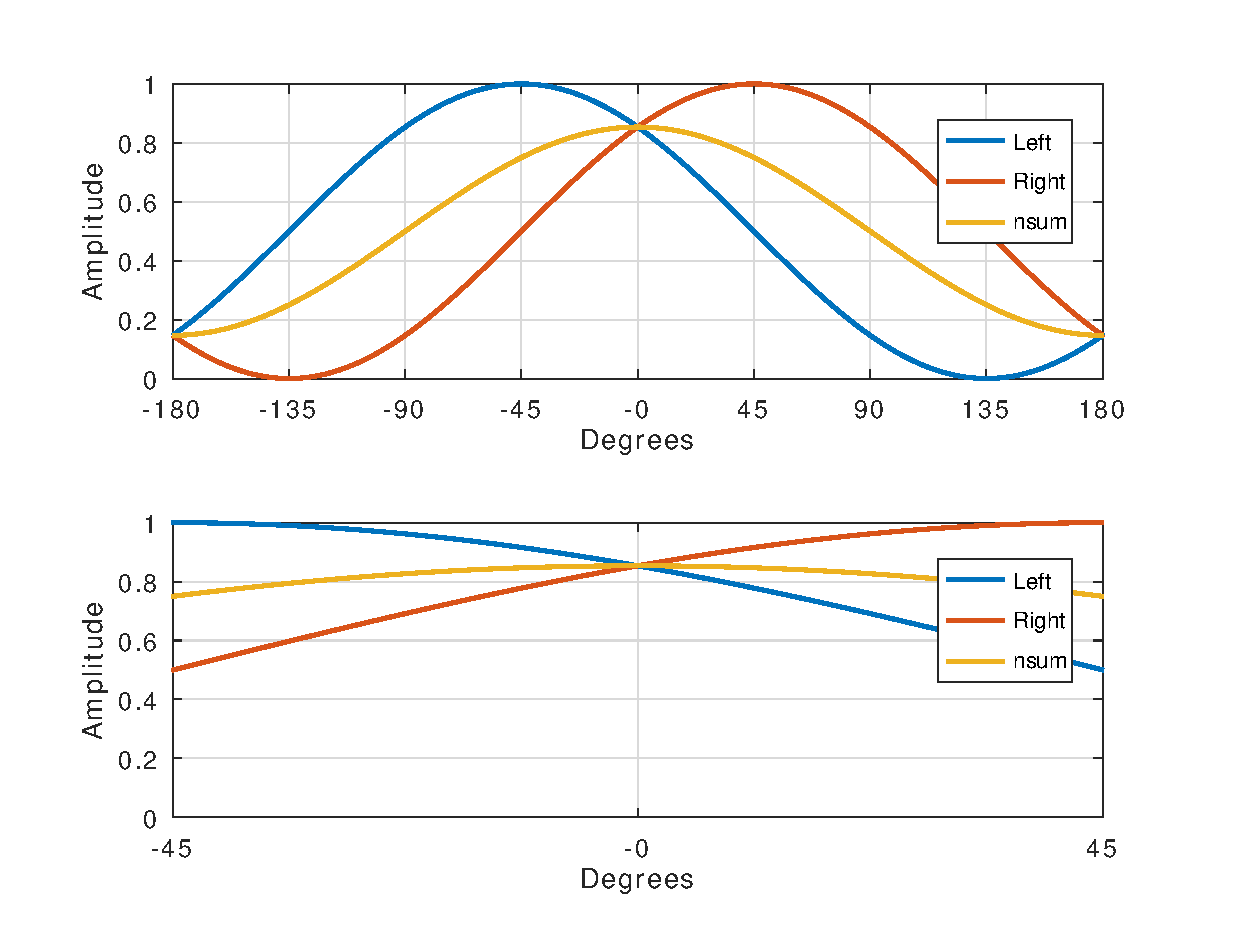
\includegraphics[width=12.5cm]{CAPITOLI/1000/IMG/xy90sub}
        \caption{Variazioni angolari di ampiezza.}% \\ Eq: $0.75(x)+0.25(x\cos\theta)$}
        \label{plot:xy90}
    \end{subfigure}
    \caption{XY90}
    \label{sp:xy90}
\end{figure*}

\clearpage

\begin{figure*}[t]
    \centering
    \begin{subfigure}[t]{0.99\textwidth}
        \centering
        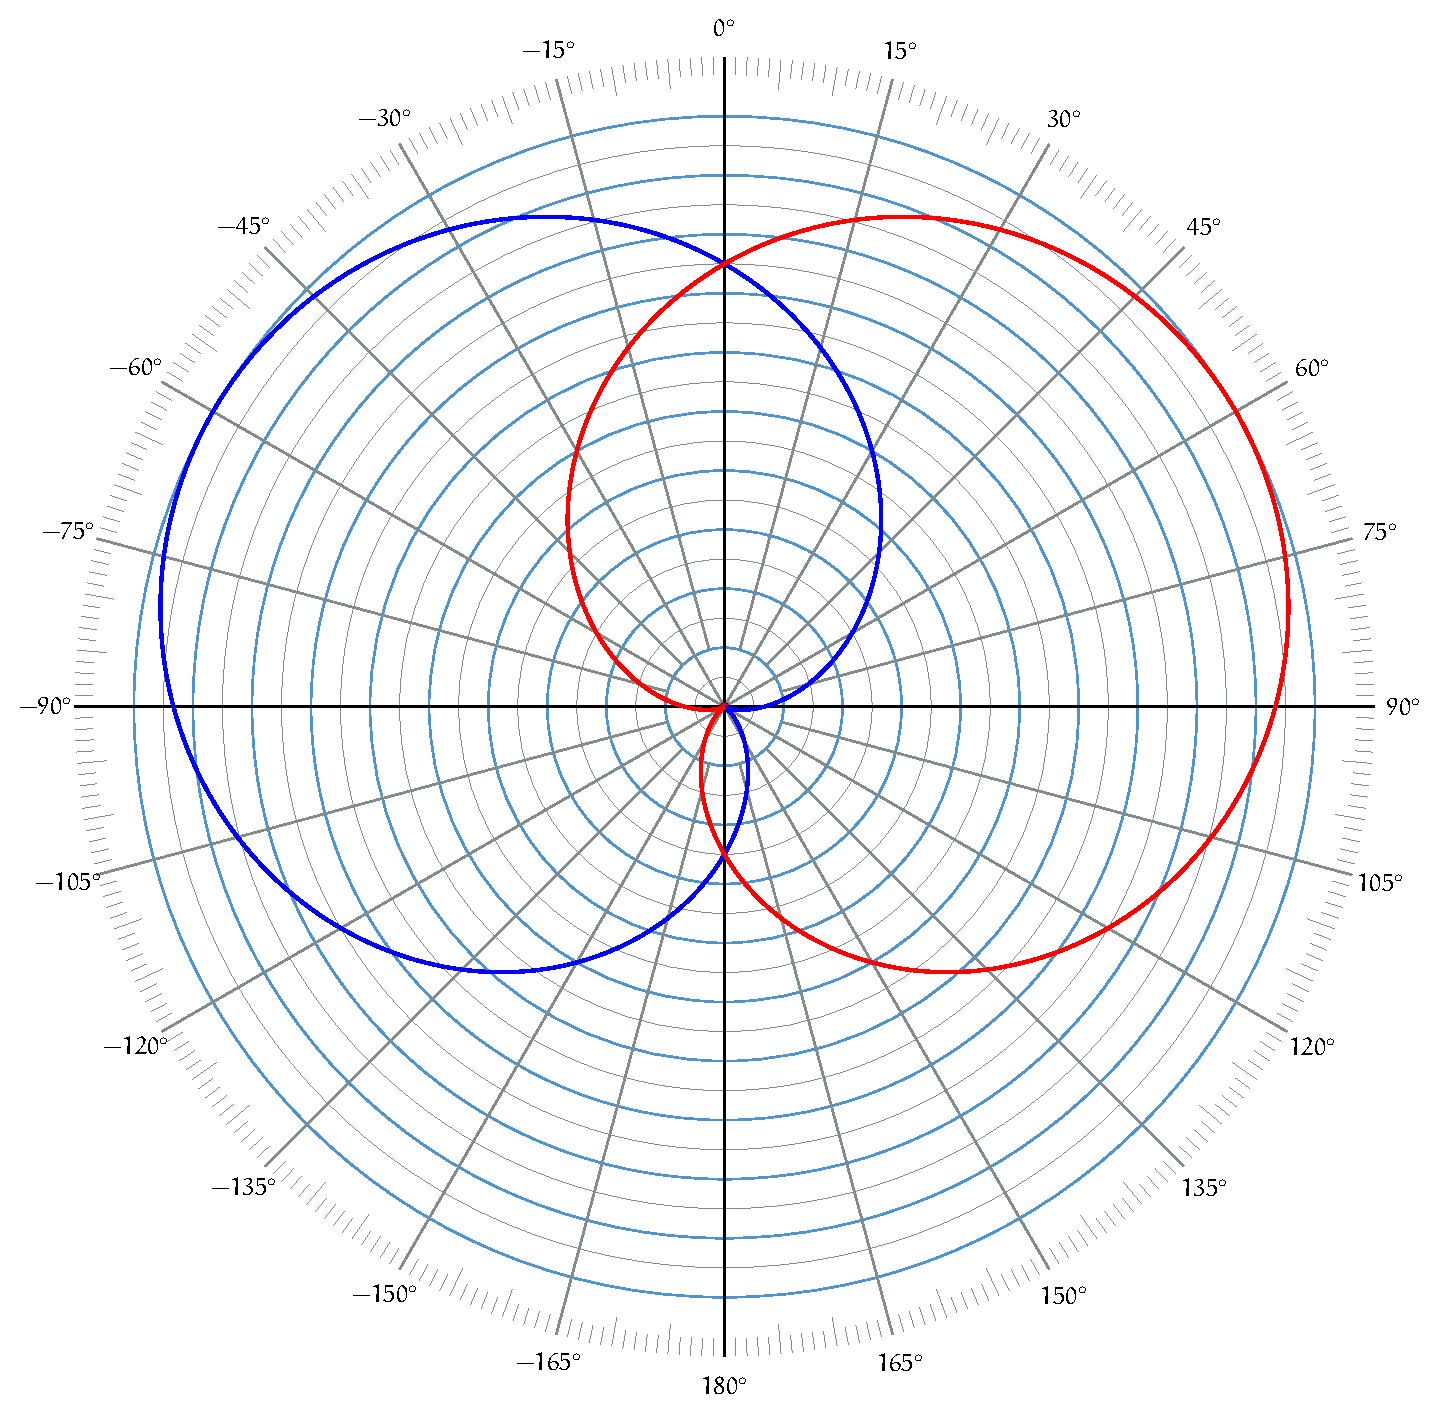
\includegraphics[width=11cm]{CAPITOLI/_TIKZ/POLAR/xy120}
        \caption{XY90. Coppia stereofonica coincidente di cardioidi angolati tra loro di $120°$.}% \\ Eq: $1(x)$}
        \label{pol:xy120sp}
    \end{subfigure}%
    \\
    \begin{subfigure}[t]{0.99\textwidth}
        \centering
        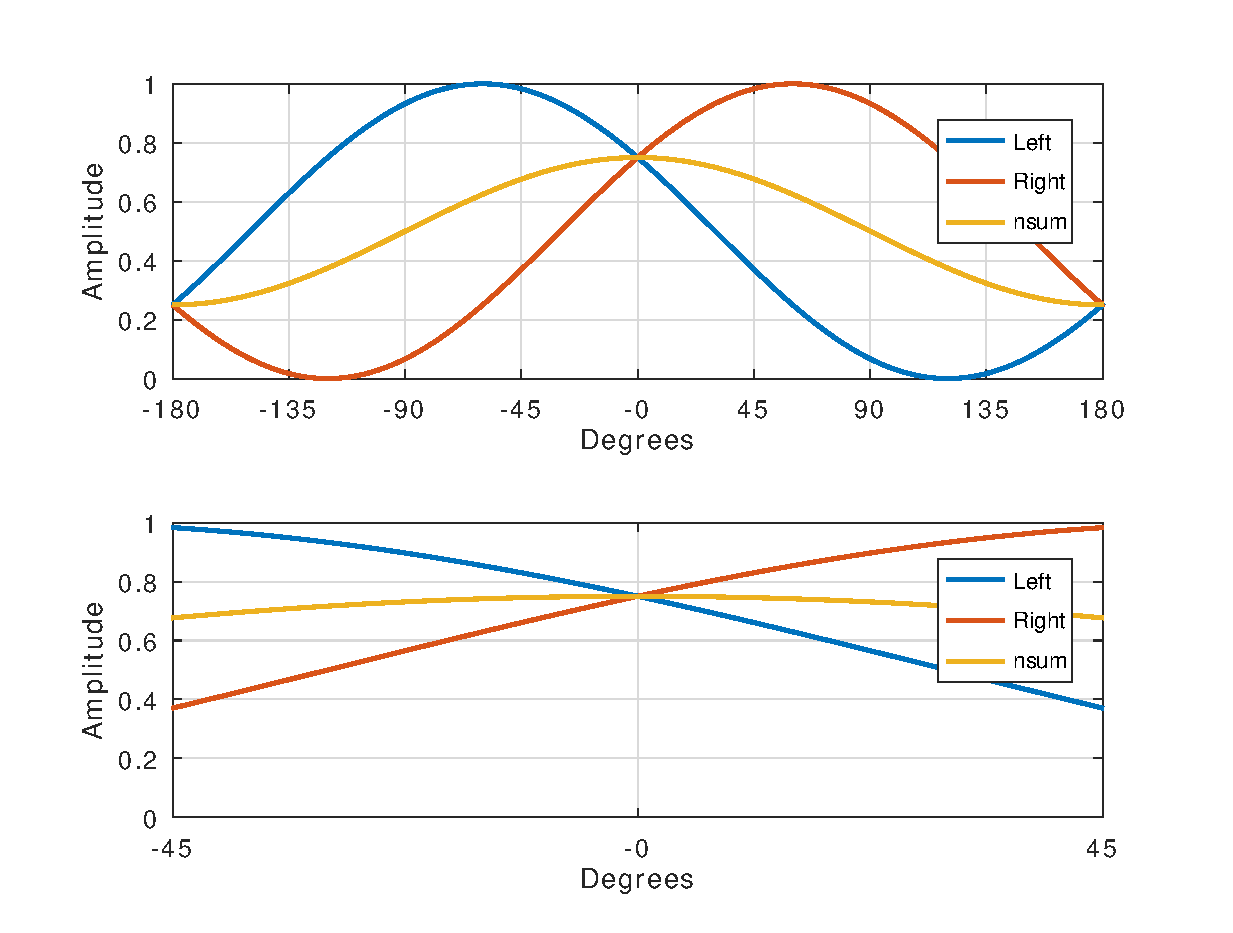
\includegraphics[width=12.5cm]{CAPITOLI/1000/IMG/xy120sub}
        \caption{Variazioni angolari di ampiezza.}% \\ Eq: $0.75(x)+0.25(x\cos\theta)$}
        \label{plot:xy120}
    \end{subfigure}
    \caption{XY120}
    \label{sp:xy120}
\end{figure*}

\clearpage

\begin{figure*}[t]
    \centering
    \begin{subfigure}[t]{0.99\textwidth}
        \centering
        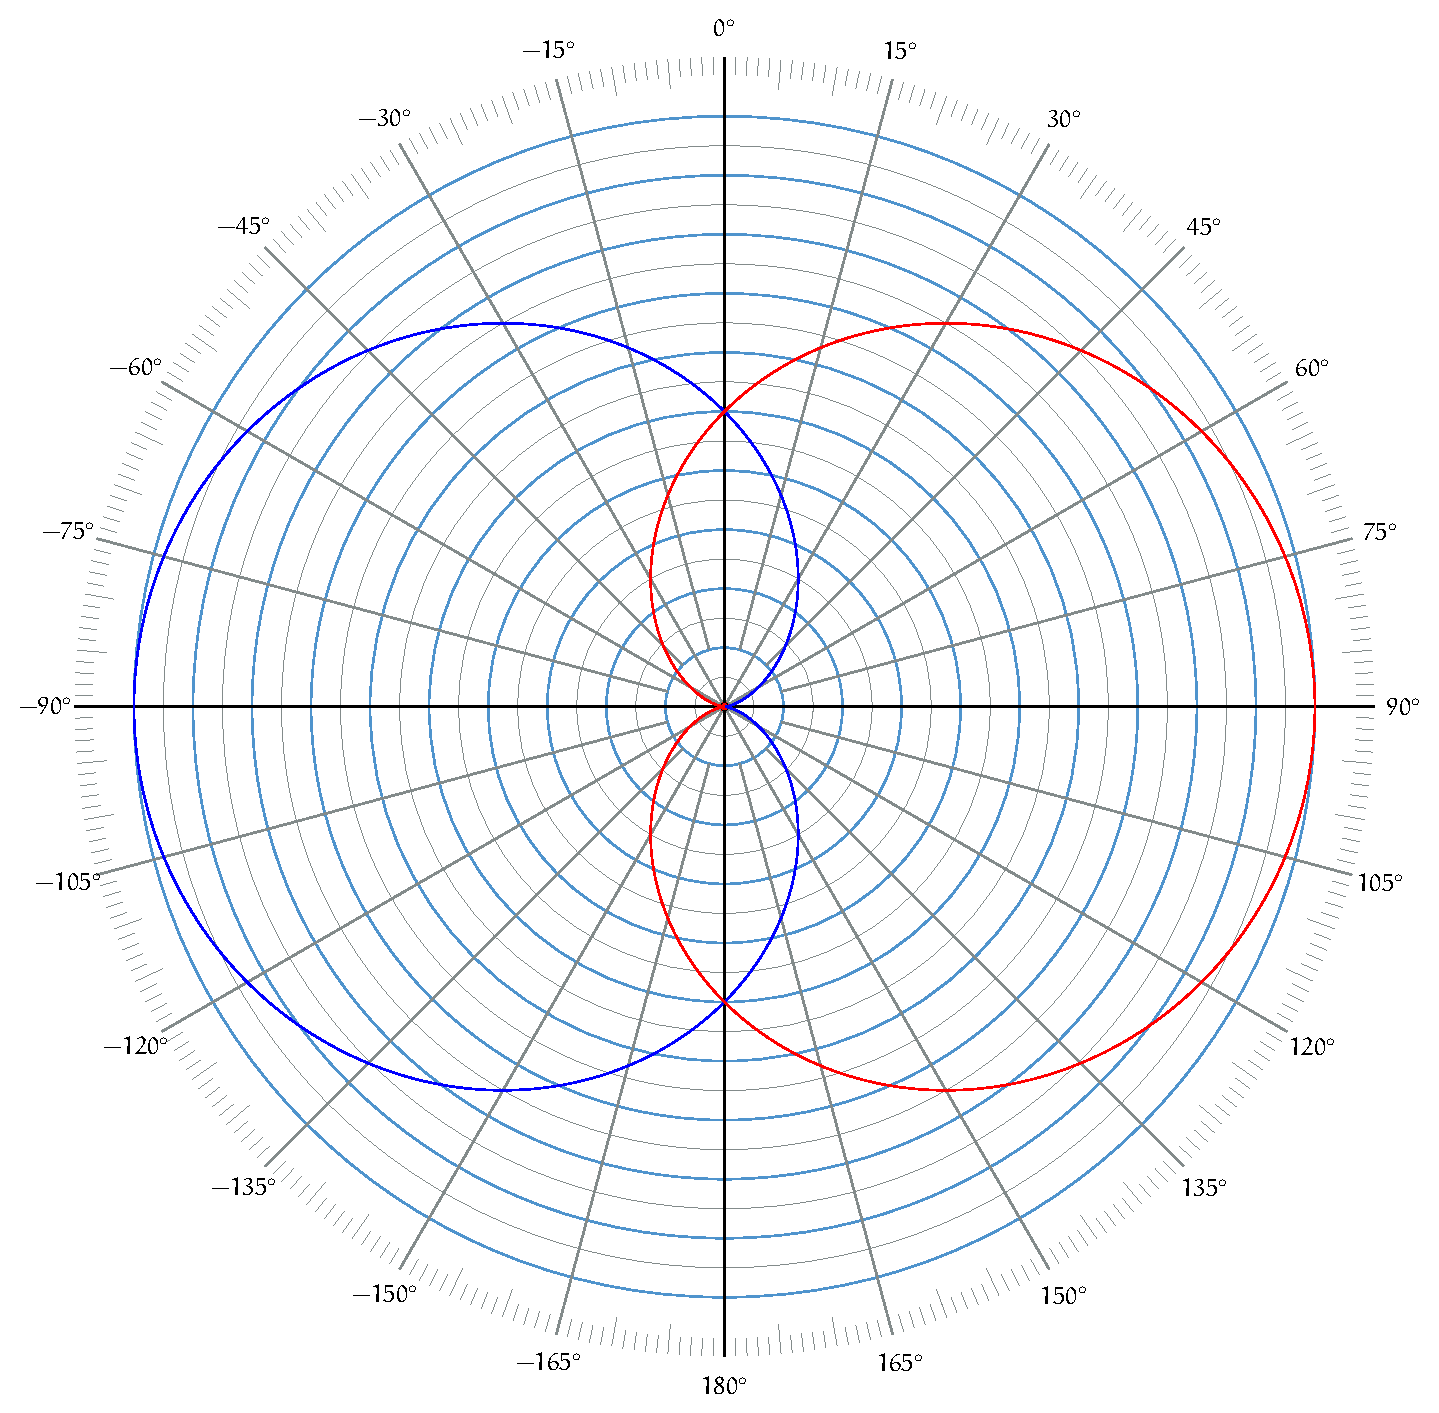
\includegraphics[width=11cm]{CAPITOLI/_TIKZ/POLAR/xy180}
        \caption{XY90. Coppia stereofonica coincidente di cardioidi angolati tra loro di $180°$.}% \\ Eq: $1(x)$}
        \label{pol:xy120sp}
    \end{subfigure}%
    \\
    \begin{subfigure}[t]{0.99\textwidth}
        \centering
        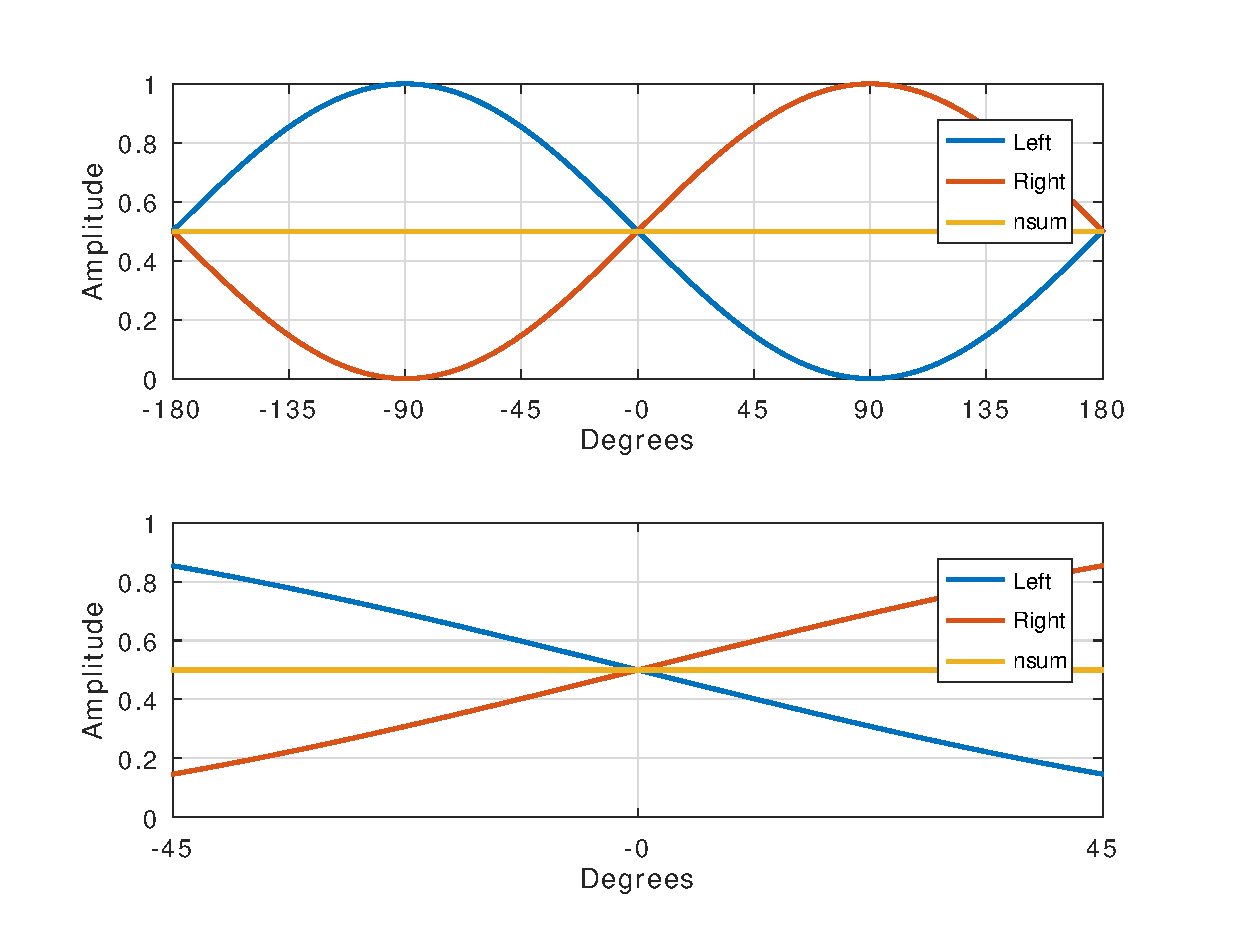
\includegraphics[width=12.5cm]{CAPITOLI/1000/IMG/xy180sub}
        \caption{Variazioni angolari di ampiezza.}% \\ Eq: $0.75(x)+0.25(x\cos\theta)$}
        \label{plot:xy180}
    \end{subfigure}
    \caption{XY180}
    \label{sp:xy180}
\end{figure*}

\clearpage

\begin{figure*}[t]
    \centering
    \begin{subfigure}[t]{0.99\textwidth}
        \centering
        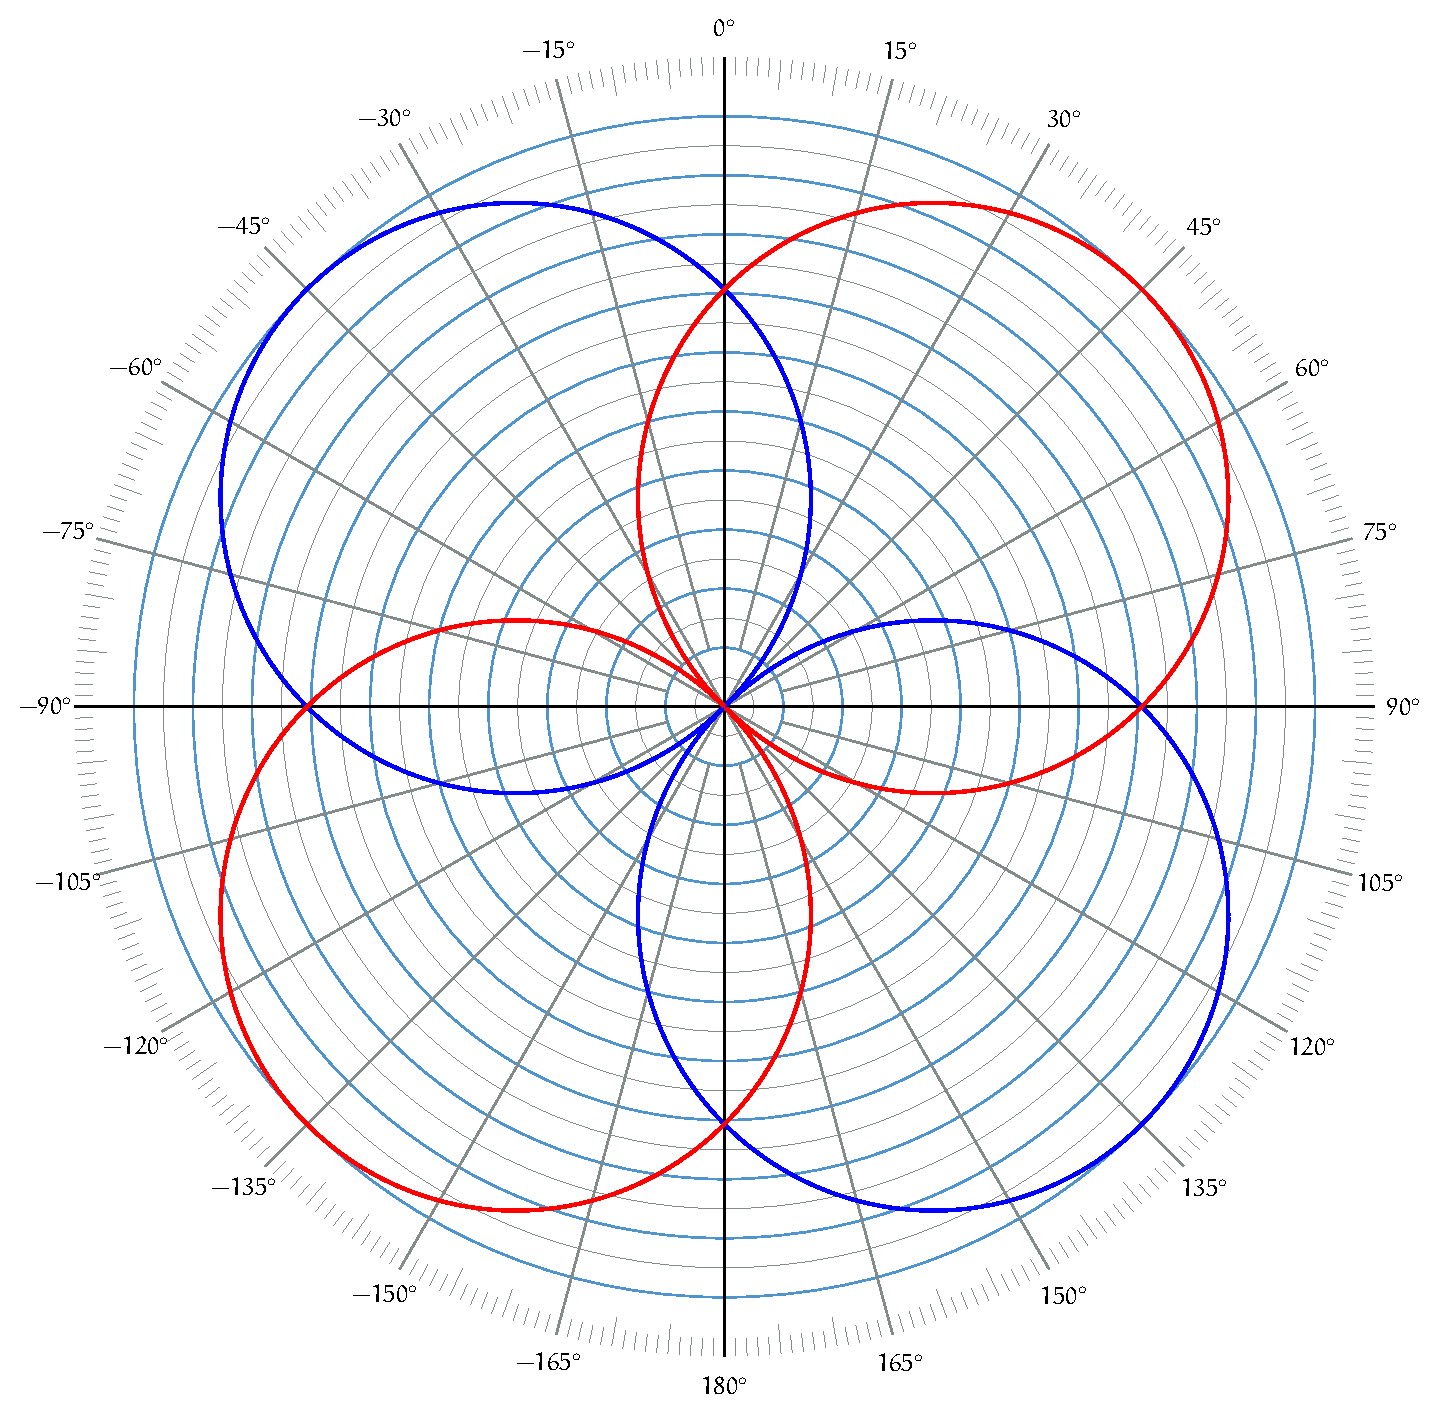
\includegraphics[width=11cm]{CAPITOLI/_TIKZ/POLAR/blumlein}
        \caption{BLUMLEIN. Coppia stereofonica coincidente di figura-8 angolati tra loro di $90°$.}% \\ Eq: $1(x)$}
        \label{pol:blumleinsp}
    \end{subfigure}%
    \\
    \begin{subfigure}[t]{0.99\textwidth}
        \centering
        \includegraphics[width=12.5cm]{CAPITOLI/1000/IMG/blumleinsub}
        \caption{Variazioni angolari di ampiezza.}% \\ Eq: $0.75(x)+0.25(x\cos\theta)$}
        \label{plot:blumlein}
    \end{subfigure}
    \caption{BLUMLEIN}
    \label{sp:blumlein}
\end{figure*}

\clearpage

\subsection{Semi-coincidenti}

\begin{figure*}[t]
    \centering
    \begin{subfigure}[t]{0.99\textwidth}
        \centering
        \includegraphics[width=11cm]{CAPITOLI/_TIKZ/POLAR/ORTF}
        \caption{ORTF. Coppia stereofonica semi-coincidente di cardioidi angolati tra loro di $110°$ e distanti $17cm$.}% \\ Eq: $1(x)$}
        \label{pol:ortfsp}
    \end{subfigure}%
    \\
    \begin{subfigure}[t]{0.99\textwidth}
        \centering
        \includegraphics[width=12.5cm]{CAPITOLI/1000/IMG/ortfsub}
        \caption{Variazioni angolari di ampiezza.}% \\ Eq: $0.75(x)+0.25(x\cos\theta)$}
        \label{plot:ortf}
    \end{subfigure}
    \caption{ORTF}
    \label{sp:ortf}
\end{figure*}


\printbibliography
\end{refsection}


\appendix

%!TEX TS-program = xelatex
%!TEX encoding = UTF-8 Unicode
% !TEX root = ../metm.tex

\chapter{Pensare il tempo}

\begin{flushright}
\textit{- Alice: How long is forever?\\
- White Rabbit: Sometimes, just one second.”}\\
Lewis Carroll, Alice in Wonderland
\end{flushright}

In questa sezione affronteremo un piccolo esercizio di programmazione che porterà
alla creazione di un semplice metronomo digitale. Lo scopo di tale esercizio è
quello di accedere alla programmazione temporizzata degli eventi sonori.

risorse necessarie:\\
\url{http://faustide.grame.fr/}

\startcontents[chapters]
\printcontents[chapters]{}{1}{}

\section{Scansioni ritmiche}

Prima di inoltrarsi nel pratico della creazione, c'è un minimo di riflessione da
fare sul come dividiamo il tempo e perché.

\begin{quote}
Da secoli, \emph{dividiamo} il tempo in giorni. La parola “tempo” deriva da una
radice indoeuropea, \emph{di} o \emph{dai}, che indica “dividere”. Da secoli,
dividiamo il giorno in ore. Per la maggior parte di questi secoli, però, le ore
erano più lunghe d'estate e più corte d'inverno, perché le 12 ore scandivano il
tempo fra alba e tramonto: l'ora prima era l'alba, e l'ora dodicesima il tramonto,
indipendentemente dalla stagione. [\ldots] È solo verso il XIII secolo che in Europa
la vita della gente comincia a essere regolata da orologi meccanici. Città e
villaggi costruiscono la loro chiesa, accanto alla chiesa il campanile, e sul
campanile un orologio che dà il ritmo alle funzioni collettive. Inizia l'era del
tempo regolato da orologi\footnote{Rovelli - l'ordine del tempo. pg 56-57}.
\end{quote}

L'idea di un tempo fluido, che non ticchetta, che non rintocca, era la consuetudine
prima degli orologi. Oggi è molto meno comune un pensiero di questo tipo. Siamo
legati ai ticchettii.
\begin{quote}
L'utilità degli orologi è indicare a tutti la stessa ora. Ma anche quest'idea è
più moderna di quanto possiamo immaginare. Per secoli, finché si viaggiava a
cavallo, a piedi o in carrozza, non c'era motivo di sincronizzare orologi da un
luogo all'altro. C'era un ottimo motivo per \emph{non} farlo: mezzodì è per
definizione quando il sole è più alto nel cielo. [\ldots] Nel XIX secolo arriva
il telegrafo, i treni diventano comuni e veloci, e il problema di sincronizzare
bene gli orologi da una città all'altra si fa importante\footnote{Rovelli - l'ordine del tempo}.
\end{quote}

Anche il metronomo ha la sua storia. Innanzitutto l'etimologia della parola,
che compare per la prima volta nel 1815 per opera di Johann Nepomuk M\"{a}lzel
mediante l'unione di due parole greche: \emph{metron}, misura e \emph{nomos}, regola.
Seppur sotto il nome di M\"{a}lzel, tanto da trovare indicazioni metronomiche
con la sigla \emph{MM} (Metronomo M\"{a}lzel), il dispositivo si basa su un
principio messo a punto da Dietrich Nikolaus Winkel, al quale M\"{a}lzel aggiunse
il tipico rintocco sonoro. Il musicista analogico sa che M\"{a}lzel e Winkel sono
rimasti a lungo due marchi importanti di metronomi meccanici.

Il metronomo meccanico si basa sui concetti dell'oscillazione pendolare:
è infatti costituito da pendolo capovolto, con un'asta graduata fra le 40 scansioni
e le 208 scansioni al minuto primo. Spostando un peso lungo l'asta graduata
selezioniamo la quantità di pulsazioni per minuto.

\section{Beat per minuto}

\emph{Quanti secondi ci sono in un minuto?} Sessanta.

\emph{Quanti minuti ci sono in un'ora?} Sessanta.

\emph{Quanti secondi ci sono in un'ora?} Tremilaseicento ($60*60$).

\emph{Quanto tempo passa tra i rintocchi di un metronomo a $108bpm$?}

L'indicazione metronomica $bpm$ \emph{(Beat per minute)} ci indica quanti rintocchi
vogliamo sentire in un minuto. Ad una quantità di $60bpm$ ascoltiamo un rintocco
sessanta volte per minuto, una scansione che corrisponde a quella dei secondi.
Il metronomo impostato a $60bpm$ produce un rintocco ogni secondo, il secondo è
la distanza che c'è tra un rintocco ed il successivo.

Il minuto è la nostra grandezza di riferimento. La nostra torta intera. Ad una
scansione di $60sec$ dividiamo, come sull'orologio, la torta in sessanta parti
uguali, e avanziamo tra una e l'altra di $1/60$ di minuto (ovvero $1sec$).
Ad una scansione di $108bpm$ (battiti per minuto) stiamo dividendo la torta in
centootto parti uguali ed avaziamo tra una parte e l'altra di $1/108$ di minuto.
Volendo individuare la distanza in secondi tra un rintocco ed il successivo non
ci resta che sostituire il minuto con l'equivalente in secondi, sessanta. La
distanza che separa un beat dal successivo ($\Delta(bpm)$) in una scansione di $108BMP$ può
essere calcolata quindi con $60/108=0,\overline{5}sec$.

\begin{equation}
\Delta(bpm) = 60/bpm (sec)
\end{equation}

Volendo aumentare il grado di precisione del calcolo precedente, ci basterà scendere
ad unità di misura più piccole del secondo, come per esempio il millesimo di secondo.

\emph{Quanti millesimi di secondo ci sono in un minuto?} Sessantamila.

\section{Metronomo}

Il metronomo digitale non può far affidamento su leggi meccaniche e masse in
movimento. Il tempo all'interno del mondo informatico si muove diversamente dagli
orologi. Per un computer non è troppo difficile portare il tempo anche in
presenza di tempi diversi, per esempio, un video multimediale può avere una scansione
di $23.976fps$ (\emph{frame per second}) e, all'interno dello stesso secondo, un suono
può avere $48000Hz$ di sample rate, ovvero essere descritto in un secondo per 48000 punti.

La frequenza di campionamento, \emph{sample rate (sr)}, nel magico mondo dei
segnali audio digitali, è la divisione del secondo per l'unità più piccola descrivibile,
il campione (\emph{sample}). Alla frequenza di campionamento di $48000Hz$ un campione
è grande $1/48000sec$. La torta, il secondo, è divisa in quarantottomila parti.

\emph{A $SR=48000$ quanti campioni ci sono in un minuto?} Due milioni e ottocentoottantamila.

Le frequenze di campionamento, seppur standardizzate, possono essere molteplici in
quanto definiscono quanto è accurata la descrizione del suono digitale nel tempo.

Dovremo riferirci ad una formula che generalizzi il valore della frequenza di campionamento
e sapere esattamente a che frequenza si esegue il calcolo, per ricavare il numero
di campioni che occorrono in ogni minuto, $spm$ (\emph{samples per minute}).

\begin{equation}
spm = SR*60
\end{equation}

Ora che il nostro orologio audio è definito nel numero di campioni che compongono
il minuto, è piuttosto semplice capire a che distanza, in campioni, avviene un
rintocco dal successivo alla velocità metronomica di $108BMP$ ad una frequenza
di campionamento di $48000Hz$, attraverso la formula $48000*60/108=26666,\overline{6}$.
È indispensabile chiarire immediatamente che per il computer non esiste, nella
descrizione del segnale audio, la parte decimale del campione, quindi di quella
dimensione terremo solo la parte intera: un rintocco ogni $26666$ campioni.

Ci sono ora i presupposti concettuali per iniziare a scrivere il codice di programma
che porterà al metronomo digitale.

%-----------------------------------------------------------
%-------------------------------larghezza massima del codice
\begin{lstlisting}
//-------------------------------------------- METRONOMO ---
//------------------------------- dichiarazioni iniziali ---
declare name "METRONOMO";
import("stdfaust.lib");
//------------------- numero di campioni per ogni minuto ---
SPM = (60*ma.SR);
\end{lstlisting}

Con le prime righe di codice abbiamo iniziato, e dato un nome, al progetto metronomo.
Il consueto \emph{import} della libreria standard ci permette di utilizzare
le funzioni standard di Faust. Con la funzione \emph{spm} otteniamo il numero di
campioni per minuto, chiendendo a Faust di verificare a che frequenza di campionamento
è impostato il computer prima di effettuare il calcolo, attraverso la funzione
matematica standard \emph{ma.SR}.

Aggiungiamo al codice precedente il selettore del valore metronomico attraverso
uno slider orizzontale

\begin{lstlisting}
//------------------------------- cursore selezione BPM ---
BPM = hslider("[01]BPM", 60, 40, 240, 0.1);
\end{lstlisting}

Ora che siamo in grado di introdurre il valore metronomico dovremo inserire
la formula che mette in relazione il numero di campioni per ogni minuto con la
quantità di BPM desiderata

\begin{lstlisting}
//-------------------------------- cursore selezione BPM ---
//-------------------- init-min--max-step-------------------
BPM = hslider("[01]BPM", 60, 40, 240, 0.1);
//------------------- numero di campioni per ogni minuto ---
SPM = (60*ma.SR);
//------------- formula di conversione da BPM a campioni ---
tempo = SPM/BPM : int; // solo la parte intera
\end{lstlisting}

Il sistema ora è in grado di fornire la distanza tra un rintocco ed il successivo
al variare dei $bpm$. Facciamolo suonare.

\begin{lstlisting}
//-------------------------------------------- METRONOMO ---
//------------------------------- dichiarazioni iniziali ---
declare name "METRONOMO";
import("stdfaust.lib");
//-------------------------------- cursore selezione BPM ---
//-------------------- init-min--max-step-------------------
BPM = hslider("[01]BPM", 60, 40, 240, 0.1);
//------------------- numero di campioni per ogni minuto ---
SPM = (60*ma.SR);
//------------- formula di conversione da BPM a campioni ---
tempo = SPM/BPM : int; // solo la parte intera
//--------------------------------- impulso temporizzato ---
metronomo = ba.pulsen(1, tempo); // (dimensione - distanza)
//------------------- METRONOMO SUI DUE CANALI DI USCITA ---
process =   metronomo <: _,_ ;
\end{lstlisting}

Il sistema funziona, agendo sul controllo BPM otteniamo quello la variazione di
distanza tra i rintocchi.

L'oggetto \emph{ba.pulsen} produce una pulsazione ad intervalli regolari.
La pulsazione può essere di grandezza variabile, così come la distanza, entrambe
le grandezze espresse in campioni. La riga

\begin{lstlisting}
//--------------------------------- impulso temporizzato ---
metronomo = ba.pulsen(1, tempo); // (dimensione - distanza)
\end{lstlisting}

genera un impulso grande un campione alla distanza in campioni espressa da \emph{tempo}
che sappiamo produrre il numero di campioni in relazione al numero di $bpm$ immesso.
L'impulso grande un campione è un clik unitario, ovvero grande la dimensione
più piccola possibile in un segnale audio ed è definito impulso.
Un impulso di questo tipo, se osservato nel dominio della frequenza contiene tutte
le frequenze dello spettro audio. In questo senso, un segnale contenente ogni
frequenza della banda audio, sprigionata in un impulso, è il segnale perfetto per
far risuonare un filtro, esattamente come farebbe una campana colpita da un martello.
A parità di martello e di energia, più la campana sarà stretta, più sarà lunga la risonanza.

\begin{lstlisting}
//---------------------------------------------- SINTESI ---
//------------------------------------- filtro risonante ---
fireson = fi.highpass(128, 1000) : fi.lowpass(8, 1000);
\end{lstlisting}

Il primo filtro è un filro passa alto del centoventottesimo ordine, intonato a
$1000Hz$ e si comporta come una campana intonata a quella frequenza. Il secondo
filtro è opposto, passa basso, serve a tenere sotto controllo la banda passante nel
versante superiore ed elimina il suono impulsivo iniziale.

Il metronomo è ora completo, di seguito il codice contenente tutti i passaggi
precedenti\footnote{Il codice completo può essere compilato online e scaricato
sul computer o direttamente sul proprio smartphone puntando il \emph{QRcode}.}.

%-----------------------------------------------------------
%-------------------------------larghezza massima del codice
\begin{lstlisting}
//-------------------------------------------- METRONOMO ---
//------------------------------- dichiarazioni iniziali ---
declare name "METRONOMO";
import("stdfaust.lib");
//-------------------------------- cursore selezione BPM ---
//-------------------- init-min--max-step-------------------
BPM = hslider("[01]BPM", 60, 40, 240, 0.1);
//------------------- numero di campioni per ogni minuto ---
SPM = (60*ma.SR);
//------------- formula di conversione da BPM a campioni ---
tempo = SPM/BPM : int; // solo la parte intera
//---------------------------------------------- SINTESI ---
//------------------------------------- filtro risonante ---
fireson = fi.highpass(128, 1000) : fi.lowpass(8, 1000);
//------------------------------------ impulso risonante ---
metronomo = ba.pulsen(1, tempo) : fireson;
//-------------------- METRONOMO SU DUE CANALI DI USCITA ---
process =   metronomo <: _,_ ;
\end{lstlisting}


%\clearpage

%\begin{longtable}{r|L{0.71\textwidth}}
  \multicolumn{2}{c}{\textbf{CLASSE V LICEO MUSICALE • I Quadrimestre}} \\
  \multicolumn{2}{c}{\textbf{I modulo Titolo: Linguaggi di programmazione, interattività e multimedialità}} \\
  \endhead
  \hline
  \textbf{Obiettivi} &
  \textbf{Conoscenze:} \newline
    Acquisire i principali strumenti critici per l'analisi dell'audiovisivo.\newline
    Conoscere le principali tecniche di produzione e post-produzione audio e musicale in relazione all'audiovisivo.\newline
    Completare la conoscenza del percorso storico della musica elettroacustica, le aree territoriali, i compositori e le relazioni storiche tra essi.\newline
    Principi di interattività, installazione, realtà virtuale, multimedialità. \newline
  \textbf{Abilità:} \newline
    Lettura e comprensione di testi della letteratura specifica, manuali operativi e utente, di strumenti di lavoro, hardware e software.\newline
    Elaborazione e produzione di progetti compositivi, sia in forma di esercizio che di produzione autonoma, in lavori di gruppo con sistemi di condivisione dati e networking.\newline
    Accesso alla stesura di strutture musicali per gli audiovisivi e le opere interattive.\newline
    Elaborazione e produzione di un repertorio elettroacustico.\newline
  \textbf{Competenze:} \newline
    Completa padronanza della terminologia specifica, degli strumenti di studio, esercizio e lavoro applicato alle tecnologie musicali.\newline
    Completa autonomia critica ed analitica di opere elettracustiche e digitali.\newline
    Completa autonomia di produzione ed elaborazione personale spontanea e su commissione. \\
  \hline
  \textbf{Contenuti} &
    La tecnologia come strumento di esercizio e lavoro applicato alle
    discipline di studio. L'approfondimento teorico e la prova sperimentale
    come approccio d'indagine. Il repertorio musicale e la letteratura come
    guida tra le tematiche d'approfondimento. \newline
    Il computer come strumento e ambiente di lavoro polifunzionale.
    Il linguaggio di programmazione come strumento di pensiero. \newline
    L'elaborazione dei suoni al computer, elaborazione strutturata di un segnale,
    le tecniche di \emph{digital signal processing - dsp}.\newline
    La notazione musicale contemporanea, suono segno ed interpretazione.\newline
    Le superfici di controllo, le automazioni i sensori, strutturazione e
    programmazione di un proprio ambiente di lavoro personalizzato. \\
  \hline
  \textbf{Metodo} &
    Lezione frontale in laboratorio. \newline
    Ogni tematica è affrontata accedendovi dal repertorio musicale.
    Si ascolta, analizza e comprende il brano di repertorio ed attraverso
    la sua applicazione musicale si approfondiscono gli argomenti emergenti.
    Si veicola quindi lo studio teorico e tecnico attraverso la pratica
    musicale, senza perdere il collegamento con il repertorio storico.
    Ogni fenomeno uditivo, percettivo e tecnologico è radicato nella
    musica del suo tempo, acquisibile mediante l'analisi, l'interpretazione
    e la pratica dello strumento tecnologico musicale. \\
  \hline
  \textbf{Tempi} &
    Mesi da Settembre a Gennaio\\
  \hline
  \textbf{Materiali} &
    Dispense, Estratti di testi in letteratura, partiture del repertorio,
    contenuti multimediali. \\
  \hline
  \textbf{Tipologia della verifica} &
    Prove pratiche sulle attività svolte durante i laboratori. \newline
    Questionari di diversa tipologia. \newline
    Verifiche orali.
\end{longtable}%

\clearpage

\begin{longtable}{r|L{0.71\textwidth}}
  \multicolumn{2}{c}{\textbf{CLASSE V LICEO MUSICALE • II Quadrimestre}} \\
  \multicolumn{2}{c}{\textbf{II modulo Titolo: Musicista e Tecnologia, competenze trasversali.}} \\
  \endhead
  \hline
  \textbf{Obiettivi} &
    \textbf{Conoscenze:} \newline
      Acquisire i principali strumenti critici per l'analisi dell'audiovisivo.  \newline
      Conoscere le principali tecniche di produzione e post-produzione audio e musicale in relazione all'audiovisivo.  \newline
      Completare la conoscenza del percorso storico della musica elettroacustica, le aree territoriali, i compositori e le relazioni storiche tra essi.  \newline
      Conoscenza delle pratiche di interattività, installazione, realtà virtuale, multimedialità.  \newline
    \textbf{Abilità:} \newline
      Elaborazione e produzione di progetti compositivi, relazioni, articoli scientifici e documentazione operativa, partiture e schede tecniche. \newline
      Elaborazione e produzione di strutture musicali per gli audiovisivi e le opere interattive.\newline
      Elaborazione e produzione di un repertorio elettroacustico. \newline
    \textbf{Competenze:} \newline
      Completa padronanza della terminologia specifica, degli strumenti di studio, esercizio e lavoro applicato alle tecnologie musicali. \newline
      Completa autonomia critica ed analitica di opere elettracustiche e digitali. \newline
      Completa autonomia di produzione ed elaborazione personale spontanea e su commissione. \\
    \hline
    \textbf{Contenuti} &
      La tecnologia come strumento di esercizio e lavoro applicato alle
      discipline di studio. L'approfondimento teorico e la prova sperimentale
      come approccio d'indagine. Il repertorio musicale e la letteratura come
      guida tra le tematiche d'approfondimento. \newline
      Il computer come strumento e ambiente di lavoro polifunzionale. \newline
      Il linguaggio di programmazione come strumento di pensiero. \newline
      L'elaborazione dei suoni al computer, elaborazione strutturata di un segnale,
      le tecniche di \emph{digital signal processing - dsp}. \newline
      La notazione musicale contemporanea, suono segno ed interpretazione. \newline
      Studio, ricerca e produzione, acquisizione dei mezzi per sviluppare il
      proprio percorso musicale. \\
    \hline
    \textbf{Metodo} &
      Lezione frontale in laboratorio. \newline
      Ogni tematica è affrontata accedendovi dal repertorio musicale.
      Si ascolta, analizza e comprende il brano di repertorio ed attraverso
      la sua applicazione musicale si approfondiscono gli argomenti emergenti.
      Si veicola quindi lo studio teorico e tecnico attraverso la pratica
      musicale, senza perdere il collegamento con il repertorio storico.
      Ogni fenomeno uditivo, percettivo e tecnologico è radicato nella
      musica del suo tempo, acquisibile mediante l'analisi, l'interpretazione
      e la pratica dello strumento tecnologico musicale. \\
    \hline
    \textbf{Tempi} &
      Mesi da Febbraio a Giugno \\
    \hline
    \textbf{Materiali} &
      Dispense, Estratti di testi in letteratura, partiture del repertorio,
      contenuti multimediali. \\
    \hline
    \textbf{Tipologia della verifica} &
      Prove pratiche sulle attività svolte durante i laboratori. \newline
      Questionari di diversa tipologia. \newline
      Verifiche orali. \newline
      Presentazione della produzione personale acquisita durante l'anno scolastico. \newline
      Prova pratica interpretazione d'insieme in forma di concerto.
  \end{longtable}%

\clearpage

\begin{longtable}{R{0.21\textwidth}|L{0.71\textwidth}}
\multicolumn{2}{c}{\textbf{CRITERIO DI SUFFICIENZA}} \\
\endhead
\hline
\multicolumn{2}{c}{L’alunno conseguirà la valutazione sufficiente quando dimostrerà di possedere:} \\
\hline
\multicolumn{2}{c}{\textbf{Nel I Quadrimestre:}} \\
\hline
Conoscenze: &
Conoscenza completa delle discipline in oggetto, del lessico specifico, degli strumenti di lavoro. \\
\hline
Abilità: &
Capacità di gestione autonoma di attività tecniche e pratiche all'interno del laboratorio, individuali e collettive. \\
\hline
Competenze: &
Competenza e lessico appropriato nel rapporto con gli strumenti di lavoro e le tecnologie. \newline
Competenza dell'ambiente virtuale al computer, dell'acquisizione e trattamento digitale dei suoni. \newline
Autonomia critica, analitica e di giudizio, d'ascolto e relazione con la musica e i media. \\
\hline
\multicolumn{2}{c}{\textbf{Nel II Quadrimestre:}} \\
\hline
Conoscenze: &
Conoscenza completa delle discipline in oggetto, del lessico specifico, degli strumenti di lavoro. \\
\hline
Abilità: &
Capacità di gestione autonoma di attività tecniche e pratiche all'interno del laboratorio, individuali e collettive. \\
\hline
Competenze: &
Competenza e lessico appropriato nel rapporto con gli strumenti di lavoro e le tecnologie. \newline
Competenza dell'ambiente virtuale al computer, dell'acquisizione e trattamento digitale dei suoni. \newline
Autonomia critica, analitica e di giudizio, d'ascolto e relazione con la musica e i media.
\end{longtable}

\clearpage


\clearpage

\printbibliography

\clearpage

\listoffigures

\clearpage

\listoftables

\clearpage

%\listofformulas

\addcontentsline{toc}{chapter}{Indice dei nomi}
\printindex

\end{document}
